% !TEX root = ./Thesis.tex
%%%%%%%%%%%%%%%%%%%%%%%%%%%%% Thesis.tex %%%%%%%%%%%%%%%%%%%%%%%%%%%%%%%
%                                                                      %
%  ---------- Master of Science Dissertation template ----------       %
%                                                                      %
%  Template for the Master Thesis according to the regulations         %
%  published by the Academic Board (Direcção Académica) at IST.        %
%                                                                      %
%  For up-to-date guide, please refer to the official website          %
%
% https://tecnico.ulisboa.pt/pt/ensino/estudar-no-tecnico/informacoes-academicas/dissertacao-de-mestrado/
%                                                                      %
%       Andre C. Marta                                                 %
%       Area Cientifica de Mecanica Aplicada e Aeroespacial            %
%       Departamento de Engenharia Mecanica                        ©    %
%       Instituto Superior Tecnico                                     %
%       Av. Rovisco Pais                                               %
%       1049-001 Lisboa                                                %©
%       Portugal                                                       %
%       Tel: +351 21 841 9469                                          %
%                        3469 (extention)                              %
%       Email: andre.marta@tecnico.ulisboa.pt                          %
%                                                                      %
%  Created:       Jan 20, 2011                                         %
%  Last Modified: JUn 29, 2022                                         %
%                                                                      %
%%%%%%%%%%%%%%%%%%%%%%%%%%%%%%%%%%%%%%%%%%%%%%%%%%%%%%%%%%%%%%%%%%%%%%%%
%  Revision history                                                    %
%  v1 - 2011/01/24 - original template                                 %
%  v2 - 2012/10/30 - new IST image and glossary support                %
%  v3 - 2013/12/10 - update according to 2012/13 official guide        %
%  v4 - 2014/02/28 - new default for bibliography style                %
%  v5 - 2014/05/07 - update according to 2013/14 official guide        %
%  v6 - 2015/07/02 - cover page format fixed,                          %
%                    contents page numbering fixed,                    %
%                    better language support,                          %
%                    enhanced examples of tables,                      %
%                    new option for appendix page numbering format,    %
%                    custom bibliography style                         %
%  v7 - 2018/02/19 - multiple citations compressed                     %
%  v8 - 2019/05/13 - added examples (pseudo-code)                      %
%  v9 - 2020/03/03 - added French language support                     %
%                    indented first paragraphs                         %
%  v10- 2021/01/29 - place caption above table                         %
%  v11- 2022/06/29 - included Declaration of original work             %
%%%%%%%%%%%%%%%%%%%%%%%%%%%%%%%%%%%%%%%%%%%%%%%%%%%%%%%%%%%%%%%%%%%%%%%%
%                                                                      %
% To generate the PDF file, type "make" at the terminal prompt.        %
%                                                                      %
% The IST template LaTeX package was created by the author             %
% and it can be downloaded from:                                       %
% https://fenix.ist.utl.pt/homepage/ist31052/                          %
%                                                                      %
% The external packages can be downloaded from                         %
% the Comprehensive TeX Archive Network at http://www.ctan.org/        %
%                                                                      %
% List of LaTex symbols:                                               %
% http://www.ctan.org/tex-archive/info/symbols/comprehensive/          %
%                                                                      %
% Help with LaTex can be found at                                      %
% http://www.giss.nasa.gov/tools/latex/ltx-2.html                      %
% http://en.wikibooks.org/wiki/LaTeX                                   %
%%%%%%%%%%%%%%%%%%%%%%%%%%%%%%%%%%%%%%%%%%%%%%%%%%%%%%%%%%%%%%%%%%%%%%%%

%%%%%%%%%%%%%%%%%%%%%%%%%%%%%%%%%%%%%%%%%%%%%%%%%%%%%%%%%%%%%%%%%%%%%%%%
%     Preamble                                                         %
%%%%%%%%%%%%%%%%%%%%%%%%%%%%%%%%%%%%%%%%%%%%%%%%%%%%%%%%%%%%%%%%%%%%%%%%

% ----------------------------------------------------------------------
%  Set the document class
% ----------------------------------------------------------------------
\documentclass[10pt,a4paper,twoside]{report}

% ----------------------------------------------------------------------
% Define external packages, language, margins, fonts and new commands
% ----------------------------------------------------------------------
%%%%%%%%%%%%%%%%%%%%%%%%%%%%%%%%%%%%%%%%%%%%%%%%%%%%%%%%%%%%%%%%%%%%%%%%
%                                                                      %
%     File: Thesis_Preamble.tex                                        %
%     Tex Master: Thesis.tex                                           %
%                                                                      %
%     Author: Israel Sother                                            %
%     Last modified: 27 May 2024                                       %
%                                                                      %
%%%%%%%%%%%%%%%%%%%%%%%%%%%%%%%%%%%%%%%%%%%%%%%%%%%%%%%%%%%%%%%%%%%%%%%%

% 'natbib' package
%
% Flexible bibliography support.
% http://www.ctan.org/tex-archive/macros/latex/contrib/natbib/
%
% > produce author-year style citations
%
%~\citet  and~\citep  for textual and parenthetical citations, respectively
%~\citet* and~\citep* that print the full author list, and not just the abbreviated one
%~\citealt is the same as~\citet but without parentheses. Similarly,~\citealp is~\citep without parentheses
%~\citeauthor
%~\citeyear
%~\citeyearpar
%
%% natbib options can be provided when package is loaded \usepackage[options]{natbib}
%%
%% Following options are valid:
%%
%%   round  -  round parentheses are used (default)
%%   square -  square brackets are used   [option]
%%   curly  -  curly braces are used      {option}
%%   angle  -  angle brackets are used    <option>
%%   semicolon  -  multiple citations separated by semi-colon (default)
%%   colon  - same as semicolon, an earlier confusion
%%   comma  -  separated by comma
%%   authoryear - for author–year citations (default)
%%   numbers-  selects numerical citations
%%   super  -  numerical citations as superscripts, as in Nature
%%   sort   -  sorts multiple citations according to order in ref. list
%%   sort&compress   -  like sort, but also compresses numerical citations
%%   compress - compresses without sorting
%%
% ******************************* SELECT *******************************
%\usepackage{natbib}          % <<<<< References in alphabetical list Correia, Silva, ...
\usepackage[numbers,sort&compress]{natbib} % <<<<< References in numbered list [1],[2],...
% ******************************* SELECT *******************************


% 'notoccite' package
%
% Prevent trouble from citations in table of contents, etc.
% http://ctan.org/pkg/notoccite
%
% > If you have~\cite com­mands in \sec­tion-like com­mands, or in \cap­tion,
%   the ci­ta­tion will also ap­pear in the ta­ble of con­tents, or list of what­ever.
%   If you are also us­ing an un­srt-like bib­li­og­ra­phy style, these ci­ta­tions will
%   come at the very start of the bib­li­og­ra­phy, which is con­fus­ing. This pack­age
%   sup­presses the ef­fect.
%
\usepackage{notoccite}


% ----------------------------------------------------------------------
% Define document language.
% ----------------------------------------------------------------------

% 'inputenc' package
%
% Accept different input encodings.
% http://www.ctan.org/tex-archive/macros/latex/base/
%
% > allows typing non-english text in LaTeX sources.
%
% ******************************* SELECT *******************************
% \usepackage[latin1]{inputenc} % <<<<< Windows
\usepackage[utf8]{inputenc}   % <<<<< Linux
\usepackage[T1]{fontenc}
% ******************************* SELECT *******************************


% 'babel' package
%
% Multilingual support for Plain TeX or LaTeX.
% http://www.ctan.org/tex-archive/macros/latex/required/babel/
%
% > sets the variable names according to the language selected
%
% ******************************* SELECT *******************************
%\usepackage[portuguese]{babel} % <<<<< Portuguese
\usepackage[english]{babel} % <<<<< English
%\usepackage[francais]{babel} % <<<<< French (requires package texlive-lang-french)
% ******************************* SELECT *******************************


% List of LaTeX variable names: \abstractname, \appendixname, \bibname,
%   \chaptername, \contentsname, \listfigurename, \listtablename, ...)
% http://www.tex.ac.uk/cgi-bin/texfaq2html?label=fixnam
%
% Changing the words babel uses (uncomment and redefine as necessary...)
%
\newcommand{\acknowledgments}{@undefined} % new LaTeX variable name
%
% > English
%
\addto\captionsenglish{\renewcommand{\acknowledgments}{Acknowledgments}}
%\addto\captionsenglish{\renewcommand{\contentsname}{Contents}}
%\addto\captionsenglish{\renewcommand{\listtablename}{List of Tables}}
%\addto\captionsenglish{\renewcommand{\listfigurename}{List of Figures}}
%\addto\captionsenglish{\renewcommand{\nomname}{Nomenclature}}
%\addto\captionsenglish{\renewcommand{\glossaryname}{Glossary}}
%\addto\captionsenglish{\renewcommand{\acronymname}{List of Acronyms}}
%\addto\captionsenglish{\renewcommand{\bibname}{References}} % Bibliography
%\addto\captionsenglish{\renewcommand{\appendixname}{Appendix}}

% > French
%
\addto\captionsfrench{\renewcommand{\acknowledgments}{Remerciements}}
%\addto\captionsfrench{\renewcommand{\contentsname}{Table des matières}}
%\addto\captionsfrench{\renewcommand{\listtablename}{Liste des tableaux}}
\addto\captionsfrench{\renewcommand{\listfigurename}{Liste des figures}} % Table des figures
%\addto\captionsfrench{\renewcommand{\nomname}{Nomenclature}}
%\addto\captionsfrench{\renewcommand{\glossaryname}{Glossaire}}
%\addto\captionsfrench{\renewcommand{\acronymname}{Liste des acronymes}}
%\addto\captionsfrench{\renewcommand{\bibname}{Bibliographie}}
%\addto\captionsfrench{\renewcommand{\appendixname}{Annexe}}

% > Portuguese
%
\addto\captionsportuguese{\renewcommand{\acknowledgments}{Agradecimentos}}
%\addto\captionsportuguese{\renewcommand{\contentsname}{Conte\'{u}do}}
%\addto\captionsportuguese{\renewcommand{\listtablename}{Lista de Figuras}}
%\addto\captionsportuguese{\renewcommand{\listfigurename}{Lista de Tabelas}}
\addto\captionsportuguese{\renewcommand{\nomname}{Lista de S\'{\i}mbolos}} % Nomenclatura
%\addto\captionsportuguese{\renewcommand{\glossary}{Gloss\'{a}rio}}
%\addto\captionsportuguese{\renewcommand{\acronymname}{Lista de Abrevia\c{c}\~{o}es}}
%\addto\captionsportuguese{\renewcommand{\bibname}{Refer\^{e}ncias}} % Bibliografia
%\addto\captionsportuguese{\renewcommand{\appendixname}{Anexo}} % Apendice


% ----------------------------------------------------------------------
% Define cover fields in both english and Portuguese.
% ----------------------------------------------------------------------
%
\newcommand{\coverThesis}{@undefined} % new LaTeX variable name
\newcommand{\coverSupervisors}{@undefined} % new LaTeX variable name
\newcommand{\coverExaminationCommittee}{@undefined} % new LaTeX variable name
\newcommand{\coverChairperson}{@undefined} % new LaTeX variable name
\newcommand{\coverSupervisor}{@undefined} % new LaTeX variable name
\newcommand{\coverMemberCommittee}{@undefined} % new LaTeX variable name
% > English
\addto\captionsenglish{\renewcommand{\coverThesis}{Thesis to obtain the Master of Science Degree in}}
\addto\captionsenglish{\renewcommand{\coverSupervisors}{Supervisor(s)}} % chktex 36
\addto\captionsenglish{\renewcommand{\coverExaminationCommittee}{Examination Committee}}
\addto\captionsenglish{\renewcommand{\coverChairperson}{Chairperson}}
\addto\captionsenglish{\renewcommand{\coverSupervisor}{Supervisor}}
\addto\captionsenglish{\renewcommand{\coverMemberCommittee}{Member of the Committee}}
% > French
\addto\captionsfrench{\renewcommand{\coverThesis}{Th\`ese pour l'obtention du Maîtrise des Sciences en}}
\addto\captionsfrench{\renewcommand{\coverSupervisors}{Directeur(s) de th\`ese}} % chktex 36
\addto\captionsfrench{\renewcommand{\coverExaminationCommittee}{Jury}}
\addto\captionsfrench{\renewcommand{\coverChairperson}{Pr\'esident}}
\addto\captionsfrench{\renewcommand{\coverSupervisor}{Directeur de th\`ese}}
\addto\captionsfrench{\renewcommand{\coverMemberCommittee}{Rapporteur}}
% > Portuguese
\addto\captionsportuguese{\renewcommand{\coverThesis}{Disserta\c{c}\~{a}o para obten\c{c}\~{a}o do Grau de Mestre em}}
\addto\captionsportuguese{\renewcommand{\coverSupervisors}{Orientador(es)}} % chktex 36
\addto\captionsportuguese{\renewcommand{\coverExaminationCommittee}{J\'{u}ri}}
\addto\captionsportuguese{\renewcommand{\coverChairperson}{Presidente}}
\addto\captionsportuguese{\renewcommand{\coverSupervisor}{Orientador}}
\addto\captionsportuguese{\renewcommand{\coverMemberCommittee}{Vogal}}


% ----------------------------------------------------------------------
% Define Declaration of original work in both english and portuguese.
% ----------------------------------------------------------------------
%
\newcommand{\declarationTitle}{@undefined} % new LaTeX variable name
\newcommand{\declarationText}{@undefined}  % new LaTeX variable name
% > English
\addto\captionsenglish{\renewcommand{\declarationTitle}{\Large\textbf{Declaration}\normalsize}}
\addto\captionsenglish{\renewcommand{\declarationText}{I declare that this document is an original work of my own authorship and that it fulfills all the requirements of the Code of Conduct and Good Practices of the Universidade de Lisboa.}}
% > Portuguese
\addto\captionsportuguese{\renewcommand{\declarationTitle}{Declara\c{c}\~{a}o}}
\addto\captionsportuguese{\renewcommand{\declarationText}{Declaro que o presente documento \'{e} um trabalho original da minha autoria e que cumpre todos os requisitos do C\'{o}digo de Conduta e Boas Pr\'{a}ticas da Universidade de Lisboa.}}


% ----------------------------------------------------------------------
% Define default and cover page fonts.
% ----------------------------------------------------------------------

% Use Arial font as default
%
\renewcommand{\rmdefault}{phv}
\renewcommand{\sfdefault}{phv}

% Define cover page fonts
%
%         encoding     family       series      shape
%  \usefont{T1}     {phv}=helvetica  {b}=bold    {n}=normal
%                   {ptm}=times      {m}=normal  {sl}=slanted
%                                                {it}=italic
% see more examples at
% https://www.overleaf.com/learn/latex/Font_typefaces
% https://tug.org/FontCatalogue/
%
\def\FontLn{% 16 pt normal
  \usefont{T1}{phv}{m}{n}\fontsize{16pt}{16pt}\selectfont}
\def\FontLb{% 16 pt bold
  \usefont{T1}{phv}{b}{n}\fontsize{16pt}{16pt}\selectfont}
\def\FontMn{% 14 pt normal
  \usefont{T1}{phv}{m}{n}\fontsize{14pt}{14pt}\selectfont}
\def\FontMb{% 14 pt bold
  \usefont{T1}{phv}{b}{n}\fontsize{14pt}{14pt}\selectfont}
\def\FontSn{% 12 pt normal
  \usefont{T1}{phv}{m}{n}\fontsize{12pt}{12pt}\selectfont}


% ----------------------------------------------------------------------
% Define page margins and line spacing.
% ----------------------------------------------------------------------

% 'geometry' package
%
% Flexible and complete interface to document dimensions.
% http://www.ctan.org/tex-archive/macros/latex/contrib/geometry/
%
% > set the page margins (2.5cm minimum in every side, as per IST rules)
%
\usepackage{geometry}	
\geometry{verbose,tmargin=2.5cm,bmargin=2.5cm,lmargin=2.5cm,rmargin=2.5cm,marginparwidth=2cm}
% \usepackage{showframe} 
% 'setspace' package
%
% Set space between lines.
% http://www.ctan.org/tex-archive/macros/latex/contrib/setspace/
%
% > allow setting line spacing (line spacing of 1.5, as per IST rules)
%
\usepackage{setspace}
\renewcommand{\baselinestretch}{1.5}


% ----------------------------------------------------------------------
% Define paragraph formating.
% ----------------------------------------------------------------------

% 'indentfirst' package
%
% Indent first paragraph after section header.
% https://ctan.org/pkg/indentfirst
%
% > indent all paragraphs (as per IST rules)
%
\usepackage{indentfirst}	


% ----------------------------------------------------------------------
% Include external packages.
% Note that not all of these packages may be available on all system
% installations. If necessary, include the .sty files locally in
% the <jobname>.tex file directory.
% ----------------------------------------------------------------------

% 'graphicx' package
%
% Enhanced support for graphics.
% http://www.ctan.org/tex-archive/macros/latex/required/graphics/
%
% > extends arguments of the \includegraphics command
%
\usepackage{graphicx}


% 'color' package
%
% Colour control for LaTeX documents.
% http://www.ctan.org/tex-archive/macros/latex/required/graphics/
%
% > defines color macros: \color{<color name>}
%
%\usepackage{color}


% 'amsmath' package
%
% Mathematical enhancements for LaTeX.
% http://www.ctan.org/tex-archive/macros/latex/required/amslatex/
%
% > American Mathematical Society plain Tex macros
%
\usepackage{amsmath}  % AMS mathematical facilities for LaTeX.
\usepackage{amsthm}   % Typesetting theorems (AMS style).
\usepackage{amsfonts} % 


% 'wrapfig' package
%
% Produces figures which text can flow around.
% http://www.ctan.org/tex-archive/macros/latex/contrib/wrapfig/
%
% > wrap figures/tables in text (i.e., Di Vinci style)
%
% \usepackage{wrapfig}


% 'subfigure' package
%
% Deprecated: Figures divided into subfigures.
% http://www.ctan.org/tex-archive/obsolete/macros/latex/contrib/subfigure/
%
% > subcaptions for subfigures
%
\usepackage{subfigure}


% 'subfigmat' package
%
% Automates layout when using the subfigure package.
% http://www.ctan.org/tex-archive/macros/latex/contrib/subfigmat/
%
% > matrices of similar subfigures
%
\usepackage{subfigmat}


% 'url' package
%
% Verbatim with URL-sensitive line breaks.
% http://www.ctan.org/tex-archive/macros/latex/contrib/url/
%
% > URLs in BibTex
%
% \usepackage{url}


% 'varioref' package
%
% Intelligent page references.
% http://www.ctan.org/tex-archive/macros/latex/required/tools/
%
% > smart page, figure, table and equation referencing
%
%\usepackage{varioref}


% 'dcolumn' package
%
% Align on the decimal point of numbers in tabular columns.
% http://www.ctan.org/tex-archive/macros/latex/required/tools/
%
% > decimal-aligned tabular math columns
%
\usepackage{dcolumn}
\newcolumntype{d}{D{.}{.}{-1}} % column aligned by the point separator '.'
\newcolumntype{e}{D{E}{E}{-1}} % column aligned by the exponent 'E'


% 'verbatim' package
%
% Reimplementation of and extensions to LaTeX verbatim.
% http://www.ctan.org/tex-archive/macros/latex/required/tools/
%
% > provides the verbatim environment (\begin{verbatim},\end{verbatim})
%   and a comment environment (\begin{comment},  \end{comment})
%
% \usepackage{verbatim}


% 'moreverb' package
%
% Extended verbatim.
% http://www.ctan.org/tex-archive/macros/latex/contrib/moreverb/
%
% > supports tab expansion and line numbering
%
% \usepackage{moreverb}



% 'nomencl' package
%
% Produce lists of symbols as in nomenclature.
% http://www.ctan.org/tex-archive/macros/latex/contrib/nomencl/
%
% The nomencl package makes use of the MakeIndex program
% in order to produce the nomenclature list.
%
% Nomenclature
% 1) On running the file through LATEX, the command \makenomenclature
%    in the preamble instructs it to create/open the nomenclature file
%    <jobname>.nlo corresponding to the LATEX file <jobname>.tex and
%    writes the information from the \nomenclature commands to this file.
% 2) The next step is to invoke MakeIndex in order to produce the
%    <jobname>.nls file. This can be achieved by making use of the
%    command: makeindex <jobname>.nlo -s nomencl.ist -o <jobname>.nls
% 3) The last step is to invoke LATEX on the <jobname>.tex file once
%    more. There, the \printnomenclature in the document will input the
%    <jobname>.nls file and process it according to the given options.
%
% http://www-h.eng.cam.ac.uk/help/tpl/textprocessing/nomencl.pdf
%
% Nomenclature (produces *.nlo *.nls files)
\usepackage{nomencl}
\makenomenclature{}


%% This will add the units
%----------------------------------------------
\newcommand{\nomunit}[1]{%
\renewcommand{\nomentryend}{\hspace*{\fill}#1}}
%----------------------------------------------
% \renewcommand{\nompreamble}{\begin{multicols}{2}}
% \renewcommand{\nompostamble}{\end{multicols}}



%
% Group variables according to their symbol type
%
\RequirePackage{ifthen} 
% \ExplSyntaxOn
% \RenewDocumentCommand\nomgroup{m}
%  {
%   \par\addvspace{1cm}
%   \item[\bfseries
%     \vrule width 0pt depth 1cm
%     \str_case:nn { #1 }
%      {
%       {A}{Physics~constants}
%       {B}{Number~sets}
%       {C}{Other~symbols}
%      }
%   ]
%  }
% \ExplSyntaxOff
% \ExplSyntaxOn
% \RenewDocumentCommand\nomgroup{1}
% {
%   \par\addvspace{1cm}
%   \item[\bfseries
%     \vrule width 0pt depth 1cm
%     \str_case:nn {#1}
%     {
%       {R}{Roman symbols1}
%       {G}{Greek symbols1}
%       {S}{Subscripts1}
%       {T}{Superscripts1}
%     }
%   ]
% }
% \ExplSyntaxOff

\ifthenelse{\equal{\languagename}{english}}%
    { % English
    \renewcommand{\nomgroup}[1]{%
      \ifthenelse{\equal{#1}{R}}{%
        \item[\textbf{Roman symbols}]}{%
        \ifthenelse{\equal{#1}{G}}{%
          \item[\textbf{Greek symbols}]}{%
          \ifthenelse{\equal{#1}{S}}{%
            \item[\textbf{Subscripts}]}{%
            \ifthenelse{\equal{#1}{T}}{%
              \item[\textbf{Superscripts}]}{}}}}}%
    }{%
    \ifthenelse{\equal{\languagename}{french}}%
    { % French
    \renewcommand{\nomgroup}[1]{%
      \ifthenelse{\equal{#1}{R}}{%
        \item[\textbf{Symbole romains}]}{%
        \ifthenelse{\equal{#1}{G}}{%
          \item[\textbf{Symboles grecs}]}{%
          \ifthenelse{\equal{#1}{S}}{%
            \item[\textbf{Indices}]}{% lettre inférieure
            \ifthenelse{\equal{#1}{T}}{%
              \item[\textbf{Exposants}]}{}}}}}% lettre supérieure
    }{ % Portuguese
    \renewcommand{\nomgroup}[1]{%
      \ifthenelse{\equal{#1}{R}}{%
        \item[\textbf{Simbolos romanos}]}{%
        \ifthenelse{\equal{#1}{G}}{%
          \item[\textbf{Simbolos gregos}]}{%
          \ifthenelse{\equal{#1}{S}}{%
            \item[\textbf{Subscritos}]}{%
            \ifthenelse{\equal{#1}{T}}{%
              \item[\textbf{Sobrescritos}]}{}}}}}%
    }}%


% 'glossary' package
%
% Create a glossary.
% http://www.ctan.org/tex-archive/macros/latex/contrib/glossary/
%
% Glossary (produces *.glo *.ist files)
\usepackage{silence}
%Disable all warnings issued by latex starting with "You have..."
% \WarningFilter{latex}{You have requested package}
\usepackage[nonumberlist]{glossaries}
% (remove blank line between groups)
% \setglossary{gloskip={}}
% (redefine glossary style file)
% \renewcommand{\istfilename}{myGlossaryStyle.ist}
\makeglossaries{}


% 'rotating' package
%
% Rotation tools, including rotated full-page floats.
% http://www.ctan.org/tex-archive/macros/latex/contrib/rotating/
%
% > show wide figures and tables in landscape format:
%   use \begin{sidewaystable} and \begin{sidewaysfigure}
%   instead of 'table' and 'figure', respectively.
%
\usepackage{rotating}


% 'hyperref' package
%
% Extensive support for hypertext in LaTeX.
% http://www.ctan.org/tex-archive/macros/latex/contrib/hyperref/
%
% > Extends the functionality of all the LATEX cross-referencing
%   commands (including the table of contents, bibliographies etc) to
%   produce \special commands which a driver can turn into hypertext
%   links; Also provides new commands to allow the user to write adhoc
%   hypertext links, including those to external documents and URLs.
%
\usepackage[pdftex]{hyperref} % enhance documents that are to be
                              % output as HTML and PDF
\hypersetup{colorlinks,       % color text of links and anchors,
                              % eliminates borders around links
%            linkcolor=red,    % color for normal internal links
            linkcolor=black,  % color for normal internal links
            anchorcolor=black,% color for anchor text
%            citecolor=green,  % color for bibliographical citations
            citecolor=black,  % color for bibliographical citations
%            filecolor=magenta,% color for URLs which open local files
            filecolor=black,  % color for URLs which open local files
%            menucolor=red,    % color for Acrobat menu items
            menucolor=black,  % color for Acrobat menu items
%            pagecolor=red,    % color for links to other pages
%            pagecolor=black,  % color for links to other pages
%            urlcolor=cyan,    % color for linked URLs
            urlcolor=black,   % color for linked URLs
%	          bookmarks=true,         % create PDF bookmarks
	          bookmarksopen=false,    % don't expand bookmarks
	          bookmarksnumbered=true, % number bookmarks
	          pdftitle={Real-time Ultra Short Horizon extension MPC for the control of a Formula Student Drive},
            pdfauthor={Israel Sother},
            pdfsubject={Real-time Ultra Short Horizon extension MPC for the control of a Formula Student Drive},
            pdfkeywords={Explicit MPC, Motor Control, Electric Vehicle, Formula Student, Horizon Extension},
            pdfstartview=FitV,
            pdfdisplaydoctitle=true}


% 'hypcap' package
%
% Adjusting the anchors of captions.
% http://www.ctan.org/tex-archive/macros/latex/contrib/oberdiek/
%
% > fixes the problem with hyperref, that links to floats points
%   below the caption and not at the beginning of the float.
%
\usepackage[figure,table]{hypcap}


% 'multirow' package
%
% Create tabular cells spanning multiple rows
% http://www.ctan.org/pkg/multirow
%
\usepackage{multirow}


% 'booktabs' package
%
% Publication quality tables in LaTeX
% http://www.ctan.org/pkg/booktabs
%
% > en­hance the qual­ity of ta­bles in LaTeX, pro­vid­ing ex­tra com­mands.
%
% \renewcommand{\arraystretch}{<ratio>} % space between rows
%
\usepackage{booktabs}
%\newcommand{\ra}[1]{\renewcommand{\arraystretch}{#1}}


% 'pdfpages' package
%
% Include PDF documents in LaTeX
% http://www.ctan.org/pkg/pdfpages
%
% > in­clu­sion of ex­ter­nal multi-page PDF doc­u­ments in LaTeX doc­u­ments.
%   Pages may be freely se­lected and sim­i­lar to psnup it is pos­si­ble to put
%   sev­eral log­i­cal pages onto each sheet of pa­per.
%
% \includepdf{filename.pdf}
% \includepdf[pages={4-9},nup=2x3,landscape=true]{filename.pdf}
%
\usepackage{pdfpages}


% 'algorithmicx' package
%
% The algorithmic style you always wanted
% https://ctan.org/pkg/algorithmicx
%
% > provides many possibilities to customizethe layout of algorithms.  You can use one of the predefined layouts(pseudocode,pascalandcand others), with or without modifications,or you can define a completely new layout for your specific needs
%
\usepackage{algorithm}
\usepackage{algpseudocode}


% ----------------------------------------------------------------------
% Define new commands to assure consistent treatment throughout document
% ----------------------------------------------------------------------

\newcommand{\ud}{\mathrm{d}}                % total derivative
\newcommand{\degree}{\ensuremath{^\circ\,}} % degrees

% Abbreviations

\newcommand{\mcol}{\multicolumn}            % table format

\newcommand{\eqnref}[1]{(\ref{#1})}
\newcommand{\class}[1]{\texttt{#1}}
\newcommand{\package}[1]{\texttt{#1}}
\newcommand{\file}[1]{\texttt{#1}}
\newcommand{\BibTeX}{\textsc{Bib}\TeX}

% Typefaces ( example: {\bf Bold text here} )
%
% > pre-defined
%   \bf % bold face
%   \it % italic
%   \tt % typewriter
%
% > newly defined
\newcommand{\tr}[1]{{\ensuremath{\textrm{#1}}}}   % text roman
\newcommand{\tb}[1]{{\ensuremath{\textbf{#1}}}}   % text bold face
\newcommand{\ti}[1]{{\ensuremath{\textit{#1}}}}   % text italic
\newcommand{\mc}[1]{{\ensuremath{\mathcal{#1}}}}  % math calygraphy
\newcommand{\mco}[1]{{\ensuremath{\mathcalold{#1}}}}% math old calygraphy
\newcommand{\mr}[1]{{\ensuremath{\mathrm{#1}}}}   % math roman
\newcommand{\mb}[1]{{\ensuremath{\mathbf{#1}}}}   % math bold face
\newcommand{\bs}[1]{\ensuremath{\boldsymbol{#1}}} % math symbol
\def\bm#1{\mathchoice{}                           % math bold
  {\mbox{\boldmath$\displaystyle#1$}}%
  {\mbox{\boldmath$#1$}}%
  {\mbox{\boldmath$\scriptstyle#1$}}%
  {\mbox{\boldmath$\scriptscriptstyle#1$}}}
\newcommand{\boldcal}[1]{{\ensuremath{\boldsymbol{\mathcal{#1}}}}}% math bold calygraphy


% xcolor
% used on tables
\usepackage[table]{xcolor}

% Derivative command
% usage: \at[\bigg]{i_q=\text{const.}}
% use \big \Big \bigg \Bigg to increase bar size
\newcommand{\at}[2][]{#1|_{#2}}

% See equation labels
% \usepackage{showkeys} % remove for final versions

% Add prefix to references based on what is referred to
\usepackage[noabbrev]{cleveref}

% Allows multicolumn, used on nomenclature
\usepackage{multicol}

% Table of Contents on start of each chapter
\usepackage[nohints]{minitoc}
\renewcommand{\kernafterminitoc}{\kern-0.1\baselineskip\kern0.1ex}
% \mtcsetfeature{minitoc}{after}{\vspace{10pt}}
% \mtcsetfeature{minitoc}{before}{\vspace{-10pt}}

% Allows the \cancelto{0}{x} function
\usepackage{cancel}

% Valign key for includegraphics with page component
\usepackage[export]{adjustbox}

% Allows use of captionof
\usepackage{subcaption}

% For adjusting minipage width and height
\usepackage{adjustbox} 


% Allows the creation of plots in LaTex
\usepackage{pgfplots}
% To increase speed of document-compilation you can configure the pgfplots package to export the figures to separate PDF files and then import them into the document: compile once, then re-use the figures. To do that, add the code shown below to the preamble:
\usepgfplotslibrary{external}
% \tikzexternalize
\usepgfplotslibrary{colorbrewer,patchplots}
\usetikzlibrary{intersections}
\pgfplotsset{compat=1.7}
\pgfplotsset{
	/pgfplots/colorbar style={
		ticklabel style={
			/pgf/number format/precision=6,
			/pgf/number format/relative*=1,
		},
	},
}
\pgfplotsset{
	contour/every contour label/.style={
		sloped,
		transform shape,
		font=\footnotesize,
		inner sep=1pt,
		every node/.style={mapped color!50!black,fill=white},
		/pgf/number format/relative={\pgfplotspointmetarangeexponent},
		/pgf/number format/precision=6,
		/pgf/number format/relative*=1,
    % \pgfmathsetmacro\labelpos{#1/200}
	}
}

\newcommand\subsubsubsection{\@startsection{paragraph}{4}{\z@}%
    {-3.25ex \@plus -1ex \@minus -0.2ex}%
    {1.5ex \@plus 0.2ex}%
    {\normalfont\normalsize\bfseries}}
\makeatother
\setcounter{secnumdepth}{3} % Include subsubsubsection in numbering
\setcounter{tocdepth}{3} % Include subsubsubsection in Table of Contents

% Allows the use of \begin{landscape} \end{landscape} to rotate the page
\usepackage{lscape}

% Allows the use of \begin{sidewaysfigure} to rotate the figure
\usepackage{rotating}


% Checks if all labels are referenced
% \usepackage{refcheck}
% %%% Infrastructure    
% \makeatletter
% \newcommand{\refcheckize}[1]{%
%   \expandafter\let\csname @@\string#1\endcsname#1%
%   \expandafter\DeclareRobustCommand\csname relax\string#1\endcsname[1]{%
%     \csname @@\string#1\endcsname{##1}\@for\@temp:=##1\do{\wrtusdrf{\@temp}\wrtusdrf{{\@temp}}}}%
%   \expandafter\let\expandafter#1\csname relax\string#1\endcsname
% }
% \newcommand{\refcheckizetwo}[1]{%
%   \expandafter\let\csname @@\string#1\endcsname#1%
%   \expandafter\DeclareRobustCommand\csname relax\string#1\endcsname[2]{%
%     \csname @@\string#1\endcsname{##1}{##2}\wrtusdrf{##1}\wrtusdrf{{##1}}\wrtusdrf{##2}\wrtusdrf{{##2}}}%
%   \expandafter\let\expandafter#1\csname relax\string#1\endcsname
% }
% \makeatother
% %%% Now we add the reference commands we want refcheck to be aware of
% \refcheckize{\cref}
% \refcheckize{\Cref}
% \refcheckizetwo{\crefrange}
% \refcheckizetwo{\Crefrange} % file "Thesis_Preamble.tex"

%%%%%%%%%%%%%%%%%%%%%%%%%%%%%%%%%%%%%%%%%%%%%%%%%%%%%%%%%%%%%%%%%%%%%%%%
%     Begin Document                                                   %
%%%%%%%%%%%%%%%%%%%%%%%%%%%%%%%%%%%%%%%%%%%%%%%%%%%%%%%%%%%%%%%%%%%%%%%%
\begin{document}

% Set plain page style (no headers, footer with centered page number)
\pagestyle{plain}

% Set roman numbering (i,ii,...) before the start of chapters
\pagenumbering{roman}

% ----------------------------------------------------------------------
%  Cover page
% ----------------------------------------------------------------------
%%%%%%%%%%%%%%%%%%%%%%%%%%%%%%%%%%%%%%%%%%%%%%%%%%%%%%%%%%%%%%%%%%%%%%%%
%                                                                      %
%     File: Thesis_FrontCover.tex                                      %
%     Tex Master: Thesis.tex                                           %
%                                                                      %
%     Author: Israel Sother                                            %
%     Last modified: 27 May 2024                                       %
%                                                                      %
%%%%%%%%%%%%%%%%%%%%%%%%%%%%%%%%%%%%%%%%%%%%%%%%%%%%%%%%%%%%%%%%%%%%%%%%

\thispagestyle{empty}

% IST Logo - Signature A
% parameters: bb=llx lly urx ury (bounding box), width=h_length, height=v_length, angle=angle, scale=factor, clip=true/false, draft=true/false. 

\includegraphics[bb=9.5cm 11cm 0cm 0cm,scale=0.29]{Figures/IST_A_CMYK_POS}

\begin{center}
%
% Figure (Image or plot)
\vspace{1.5cm}
% height = 50 mm
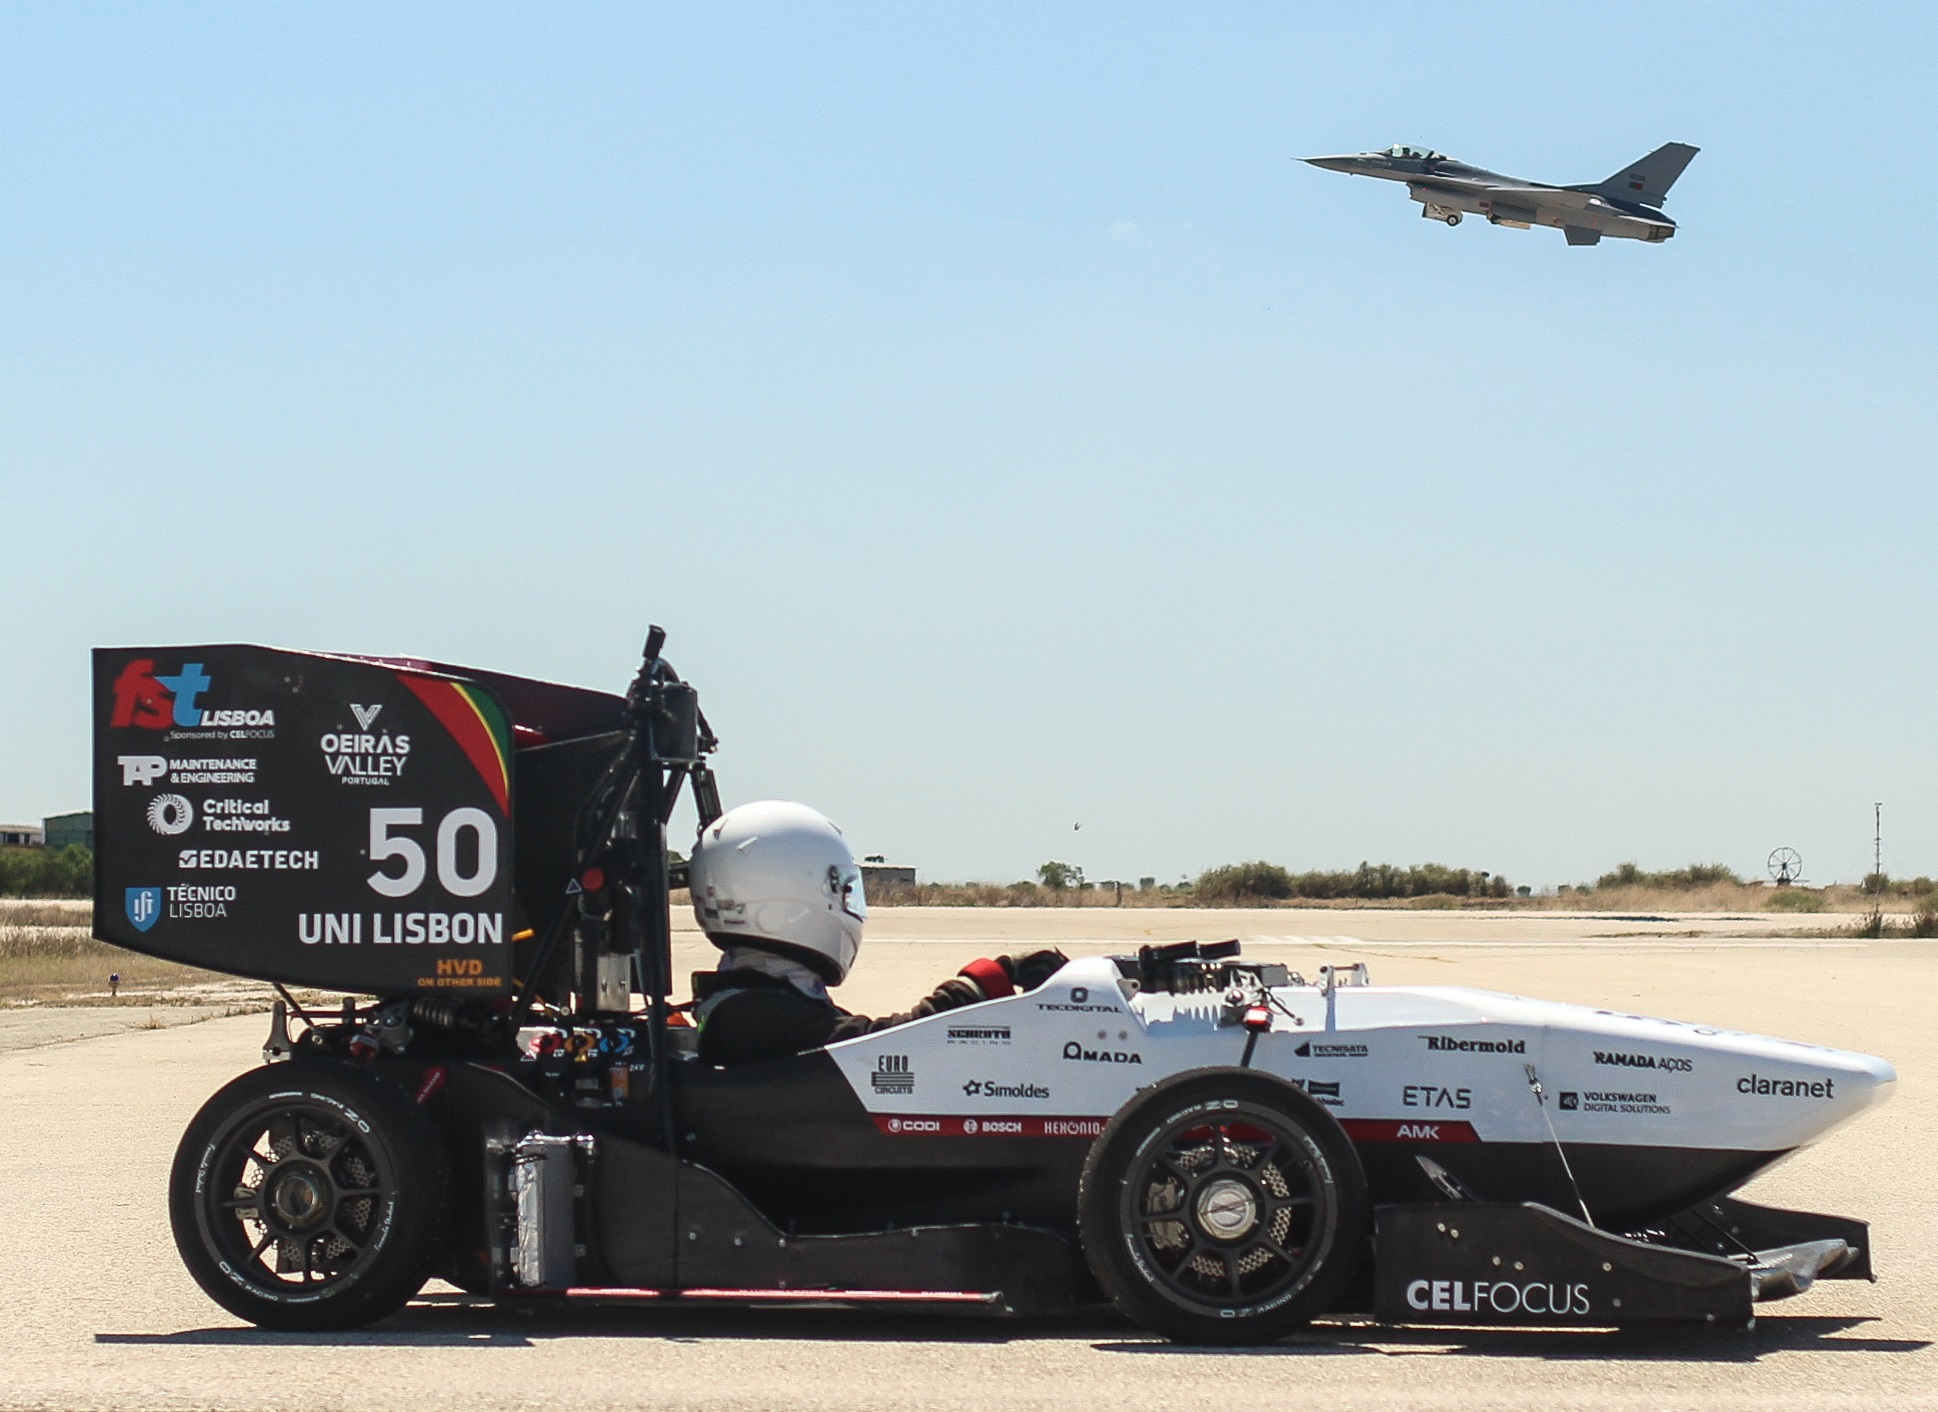
\includegraphics[height=60mm]{Figures/IMG_8888.jpg}

% Title, author and degree
\vspace{1.0cm}
{\FontLb{} Real-time Ultra Short Horizon extension MPC for the control of a Formula Student Drive} \\ % <<<<< EDIT TITLE
%\vspace{0.2cm}
%{\FontMn Subtitle (optional)} \\
%\vspace{1.9cm}
\vspace{2cm}
{\FontMb{} Israel Melo Sother} \\ % <<<<< EDIT NAME
\vspace{2.0cm}
{\FontSn{} \coverThesis} \\
\vspace{0.3cm}
{\FontLb{} Electrical and Computer Engineering} \\ % <<<<< EDIT COURSE
\vspace{1.0cm}
{\FontSn{} %
\begin{tabular}{ll}
 \coverSupervisors: & Prof. Sónia Maria Nunes dos Santos Paulo Ferreira Pinto \\ % <<<<< EDIT NAME
                    & Egn. Pedro Miguel Batista de Sousa Correia da Costa   % <<<<< EDIT NAME
\end{tabular} } \\
\vspace{1.0cm}
{\FontMb{} \coverExaminationCommittee} \\
\vspace{0.3cm}
{\FontSn{} %
\begin{tabular}{c}
\coverChairperson:     Prof. Célia Maria Santos Cardoso de Jesus   \\ % <<<<< EDIT NAME
\coverSupervisor:      Prof. Sónia Maria Nunes dos Santos Paulo Ferreira Pinto \\ % <<<<< EDIT NAME
\coverMemberCommittee: Prof. Miguel Cabral Ferreira Chaves      % <<<<< EDIT NAME
\end{tabular} } \\
\vspace{1.5cm}
{\FontMb{} May 2024} \\ % <<<<< EDIT DATE (corresponds to date of oral examination)
%
\end{center}

 % file "Thesis_FrontCover.tex"
% \cleardoublepage{}
\newpage

% ----------------------------------------------------------------------
% Dedication page (optional)
% ----------------------------------------------------------------------
%%%%%%%%%%%%%%%%%%%%%%%%%%%%%%%%%%%%%%%%%%%%%%%%%%%%%%%%%%%%%%%%%%%%%%%%
%                                                                      %
%     File: Thesis_Dedication.tex                                      %
%     Tex Master: Thesis.tex                                           %
%                                                                      %
%     Author: Israel Sother                                            %
%     Last modified: 27 May 2024                                       %
%                                                                      %
%%%%%%%%%%%%%%%%%%%%%%%%%%%%%%%%%%%%%%%%%%%%%%%%%%%%%%%%%%%%%%%%%%%%%%%%

\null\vskip5cm%
\begin{flushright}
     Dedicated to my family.
\end{flushright}
\vfill\newpage

 % file "Thesis_Dedication.tex"
% \cleardoublepage{}
\newpage

% ----------------------------------------------------------------------
% Declaration page (mandatory)
% ----------------------------------------------------------------------
%%%%%%%%%%%%%%%%%%%%%%%%%%%%%%%%%%%%%%%%%%%%%%%%%%%%%%%%%%%%%%%%%%%%%%%%
%                                                                      %
%     File: Thesis_Declaration.tex                                     %
%     Tex Master: Thesis.tex                                           %
%                                                                      %
%     Author: Israel Sother                                            %
%     Last modified: 27 May 2024                                       %
%                                                                      %
%%%%%%%%%%%%%%%%%%%%%%%%%%%%%%%%%%%%%%%%%%%%%%%%%%%%%%%%%%%%%%%%%%%%%%%%

\null\vskip5cm%
\begin{flushleft}
	\declarationTitle \\
	\declarationText
\end{flushleft}
\vfill\newpage

 % file "Thesis_Declaration.tex"
% \cleardoublepage{}
\newpage

% ----------------------------------------------------------------------
%  Acknowledgments (optional)
% ----------------------------------------------------------------------
%%%%%%%%%%%%%%%%%%%%%%%%%%%%%%%%%%%%%%%%%%%%%%%%%%%%%%%%%%%%%%%%%%%%%%%%
%                                                                      %
%     File: Thesis_Acknowledgments.tex                                 %
%     Tex Master: Thesis.tex                                           %
%                                                                      %
%     Author: Israel Sother                                            %
%     Last modified: 27 May 2024                                       %
%                                                                      %
%%%%%%%%%%%%%%%%%%%%%%%%%%%%%%%%%%%%%%%%%%%%%%%%%%%%%%%%%%%%%%%%%%%%%%%%

\section*{\acknowledgments}

% Add entry in the table of contents as section
\addcontentsline{toc}{section}{\acknowledgments}

First and foremost, I would like to express my gratitude to my supervisors, Prof. Sónia Pinto and Eng. Pedro Costa. I am extremely grateful to Prof. Sónia for her constant support and belief in me. She graciously accepted to supervise me under unusual academic circumstances, navigating the complexities of my double degree program with its confusing regulations. Words cannot express my gratitude to Eng. Pedro Costa, our numerous discussions went beyond academic mentoring; he not only introduced me to new concepts and directed my research but also provided crucial advice on balancing the transition out of the Formula Student life. I am deeply thankful for his technical expertise and the personal sacrifices he made to continue mentoring me.

Special thanks to Guilherme and Sergio for welcoming me to their day-to-day work in the office and for the countless hours spent discussing diverse topics.

I would like to express my heartfelt gratitude to my friends for their support throughout my work. They endured my constant focus on my research with steadfast companionship and encouragement, helping me remember the importance of setting aside time to clear my head, which was invaluable during this journey. Thanks also to Nuti and Mística for introducing me to the Formula Student world and to my group of friends from USP — Major, Comum, Y, and Soja — for all the moments together. Thank you for sharing with me some of the best years of my life.

To the FST11 and FST12 teams, your passionate dedication, tireless efforts, and countless late-night shifts were exhilarating. Together, we conquered numerous challenges and celebrated historic victories. It was an absolute pleasure to work side by side with some of the best engineers I have ever known. The memories we created together will always hold a special place in my heart and serve as a source of inspiration throughout my journey. I would like to extend my sincere thanks to a few members who became my closest friends during this period, Bruno, Duarte, Zé, Pedro, and Luis, your partnership and willingness to entertain all the crazy ideas we discussed were heartwarming, you made me feel welcome in a foreign country. Thank you all for making these years an unforgettable and extraordinary experience.

Lastly, I would be remiss in not mentioning my deepest gratitude to my family for their unwavering support and the sacrifices they made to enable me to study abroad. Choosing to pursue my education here meant greater physical distance between us, and I missed them every moment. I also want to acknowledge their understanding and patience during my Formula Student years, knowing that I dedicated far less time to them than I should have. Despite this, they supported me and embraced my passion for those cars, recognizing the lost time as an investment in something I love, and in turn, they learned to love it too. A special thank you to my sister, who consistently checked in on me and cared for my well-being, providing the much-needed boost when the days and nights of work blended into one. To my parents, thank you for being my role models and for always encouraging me to pursue my dreams wherever they led. Completing this degree is a testament to the values and education you instilled in me.

None of this would be possible without these incredible people. I am fortunate to have had their support and encouragement throughout my dissertation journey, and for that, I am deeply grateful. % file "Thesis_Acknowledgements.tex"
% \cleardoublepage{}
\newpage

% ----------------------------------------------------------------------
%  Abstract (both in English and Portuguese)
% ----------------------------------------------------------------------
%%%%%%%%%%%%%%%%%%%%%%%%%%%%%%%%%%%%%%%%%%%%%%%%%%%%%%%%%%%%%%%%%%%%%%%%
%                                                                      %
%     File: Thesis_Resumo.tex                                          %
%     Tex Master: Thesis.tex                                           %
%                                                                      %
%     Author: Andre C. Marta                                           %
%     Last modified :  2 Jul 2015                                      %
%                                                                      %
%%%%%%%%%%%%%%%%%%%%%%%%%%%%%%%%%%%%%%%%%%%%%%%%%%%%%%%%%%%%%%%%%%%%%%%%

\section*{Resumo}

% Add entry in the table of contents as section
\addcontentsline{toc}{section}{Resumo}

Este trabalho apresenta o desenvolvimento de uma estratégia de controlo para os motores da Equipe de Fórmula Estudantil do Instituto Superior Técnico. A estratégia de controlo foi desenvolvida para melhorar a resposta dinâmica do torque do motor e a eficiência do sistema. O motor foi caracterizado experimentalmente e um ambiente de simulação foi criado para testar diferentes estratégias de controlo. O \gls{mpc} explícito foi selecionado como a estratégia mais adequada devido à sua resposta rápida e baixa variação de corrente. Uma nova técnica de extensão de horizonte foi proposta para reduzir os erros na previsão, o que deu nome ao controlador: \acrfull{rush}. A estratégia de controlo foi implementada numa \gls{fpga} e foi desenvolvida uma bancada de testes. Os resultados experimentais mostraram uma correspondência próxima com os resultados da simulação, validando a estimativa de torque, as medições de corrente e a estratégia de controlo. A eficiência do sistema foi melhorada devido à redução na \gls{thd} de corrente e a resposta de torque foi melhorada em ordens de magnitude em comparação com a solução atual.

\vfill

\textbf{\Large Palavras-chave:} MPC Explícito, RUSH MPC, Controlo de Motores, Veículos Elétricos, Fórmula Estudantil, Extensão de Horizonte

   % file "Thesis_Resumo.tex"
% \cleardoublepage{}
\newpage

%%%%%%%%%%%%%%%%%%%%%%%%%%%%%%%%%%%%%%%%%%%%%%%%%%%%%%%%%%%%%%%%%%%%%%%%
%                                                                      %
%     File: Thesis_Abstract.tex                                        %
%     Tex Master: Thesis.tex                                           %
%                                                                      %
%     Author: Israel Sother                                            %
%     Last modified: 27 May 2024                                       %
%                                                                      %
%%%%%%%%%%%%%%%%%%%%%%%%%%%%%%%%%%%%%%%%%%%%%%%%%%%%%%%%%%%%%%%%%%%%%%%%

\section*{Abstract}

% Add entry in the table of contents as section
\addcontentsline{toc}{section}{Abstract}

This work presents the development of a control strategy for the motors of the Formula Student Team of Instituto Superior Técnico. The control strategy was developed with the main goal of improving the dynamic response of the motor torque and the system efficiency. The motor was experimentally characterized and a simulation environment was created to test different control strategies. The explicit \gls{mpc} was selected as the most suitable strategy due to its fast response and low current ripple. A novel horizon extension technique was proposed to reduce model mismatch, which gave the name of the controller: \acrfull{rush}. The control strategy was implemented in an \gls{fpga} and a test bench setup was developed. The experimental results showed a close match with the simulation results, validating the torque estimation, the current measurements, and the control strategy. The system efficiency was improved due to the reduction in current \gls{thd} and the torque response was improved by orders of magnitude compared to the current solution.
\vfill

\textbf{\Large Keywords:} Explicit MPC, RUSH MPC, Motor Control, Electric Vehicle, Formula Student, Horizon Extension % file "Thesis_Abstract.tex"
% \cleardoublepage{}
\newpage

% ----------------------------------------------------------------------
%  Table of contents, list of tables, list of figures and nomenclature
% ----------------------------------------------------------------------

% Table of contents
%

\dominitoc% Initialization
\tableofcontents
% \cleardoublepage{}
\newpage

% List of tables
%
% Add entry in the table of contents as section
\phantomsection{}
\addcontentsline{toc}{section}{\listtablename}
% Generate list
\listoftables
% \cleardoublepage{} 
\newpage

% List of figures
%
% Add entry in the table of contents as section
\phantomsection{}
\addcontentsline{toc}{section}{\listfigurename}
% Generate list
\listoffigures
% \cleardoublepage{} 
\newpage

% Nomenclature
%
% entries of nomenclature list
%%%%%%%%%%%%%%%%%%%%%%%%%%%%%%%%%%%%%%%%%%%%%%%%%%%%%%%%%%%%%%%%%%%%%%%%
%                                                                      %
%     File: Thesis_Nomenclature.tex                                    %
%     Tex Master: Thesis.tex                                           %
%                                                                      %
%     Author: Israel Sother                                            %
%     Last modified: 27 May 2024                                       %
%                                                                      %
%%%%%%%%%%%%%%%%%%%%%%%%%%%%%%%%%%%%%%%%%%%%%%%%%%%%%%%%%%%%%%%%%%%%%%%%
%
% The definitions can be placed anywhere in the document body
% and their order is sorted by <symbol> automatically when
% calling makeindex in the makefile
%
% The \glossary command has the following syntax:
%
% \glossary{entry}
%
% The \nomenclature command has the following syntax:
%
% \nomenclature[<prefix>]{<symbol>}{<description>}
%
% where <prefix> is used for fine-tuning the sort order,
% <symbol> is the symbol to be described, and <description> is
% the actual description.

% ----------------------------------------------------------------------
% Roman symbols [r]
\nomenclature[ri_x]{$i_x$}{Current}
\nomenclature[rE_x]{$E_x$}{Back EMF}
\nomenclature[ru_x]{$u_x$}{Voltage}
\nomenclature[rr_x]{$r_x$}{Phase resistance}
\nomenclature[rL_x]{$L_x$}{Phase self inductance}
\nomenclature[rM_xy]{$M_{xy}$}{Phase mutual inductance}
\nomenclature[rT_e]{$T_e$}{Electromagnetic torque}
\nomenclature[rT_load]{$T_{load}$}{Load reaction torque}
\nomenclature[rT_loss]{$T_{loss}$}{Losses equivalent torque}
\nomenclature[rp]{$p$}{Number of pole pairs}
\nomenclature[rh]{$h$}{Sampling time}
\nomenclature[rk]{$k$}{Discrete time index}
\nomenclature[rm]{$m$}{Modulation index}
\nomenclature[rVref]{$V_{ref}$}{Voltage reference vector}
\nomenclature[rK_v]{$K_v$}{Voltage Constant}
\nomenclature[rK_t]{$K_t$}{Torque Constant}
\nomenclature[rJ]{$J$}{Rotational Inertia}
\nomenclature[rv]{$v$}{Car Velocity}
\nomenclature[rAref]{$A_{r}$}{Car frontal reference area}
\nomenclature[rCd]{$C_{d}$}{Drag coefficient}
\nomenclature[rCr]{$C_{r}$}{Rolling resistance coefficient}
\nomenclature[rmcar]{$m_{car}$}{Car mass}
\nomenclature[rrtire]{$r_{tire}$}{Tire radius}
\nomenclature[rGr]{$G_{r}$}{Transmission Gear Ratio}
\nomenclature[rJ]{$\mathcal{J}$}{MPC cost function}
\nomenclature[rCs]{$\mathcal{C}_{soft}$}{MPC soft contraint}
\nomenclature[rs_x]{$s_x$}{MPC cost gains}
\nomenclature[rk_p]{$k_p$}{PI proportional gain}
\nomenclature[rk_i]{$k_i$}{PI integral gain}
% ----------------------------------------------------------------------
% Greek symbols [g]
\nomenclature[gtheta_e]{$\theta_e$}{Rotor electrical position}
\nomenclature[gtheta]{$\theta$}{Rotor position}
\nomenclature[gomega_e]{$\omega_e$}{Rotor electrical velocity}
\nomenclature[gomega]{$\omega$}{Rotor velocity}
\nomenclature[gomega]{$\omega_{wheels}$}{Wheel rotational velocity}
\nomenclature[gpsi]{$\psi_x$}{Flux linkage}
\nomenclature[glambda]{$\lambda$}{Lagrange Multiplier}
\nomenclature[grho]{$\rho$}{Air density}
\nomenclature[geta]{$\eta$}{Efficiency}
\nomenclature[gtau]{$\tau$}{Time Constant}


% ----------------------------------------------------------------------
% Subscripts [s]
\nomenclature[sp]{$a, b, c$}{Phase values}
\nomenclature[sl]{$A, B, C$}{Line values}
\nomenclature[sdq0]{$d, q, 0$}{Direct axis, quadrature axis, and zero-sequence components}
\nomenclature[spm]{$PM$}{Permanent Magnet component}
\nomenclature[sf]{$f,r$}{Front and Rear axle}

% ----------------------------------------------------------------------
% Superscripts [t]
\nomenclature[tT]{T}{Transpose}
\nomenclature[t]{$\dot{}$}{Time derivative}


 % file "Thesis_Nomenclature.tex"
%
% Add entry in the table of contents as section
\phantomsection{}
\addcontentsline{toc}{section}{\nomname}
% Insert glossary/nomenclature section produced by MakeIndex
% \begin{multicols}{2}
    \printnomenclature{}
% \end{multicols}
    % \cleardoublepage{}
\newpage

% entries of glossary list
%%%%%%%%%%%%%%%%%%%%%%%%%%%%%%%%%%%%%%%%%%%%%%%%%%%%%%%%%%%%%%%%%%%%%%%%
%                                                                      %
%     File: Thesis_Glossary.tex                                        %
%     Tex Master: Thesis.tex                                           %
%                                                                      %
%     Author: Israel Sother                                            %
%     Last modified: 27 May 2024                                       %
%                                                                      %
%%%%%%%%%%%%%%%%%%%%%%%%%%%%%%%%%%%%%%%%%%%%%%%%%%%%%%%%%%%%%%%%%%%%%%%%
%
% The definitions can be placed anywhere in the document body
% and their order is sorted by <symbol> automatically when
% calling makeindex in the makefile
%
% The \glossary command has the following syntax:
%
% \glossary{entry}
%
% The \nomenclature command has the following syntax:
%
% \nomenclature[<prefix>]{<symbol>}{<description>}
%
% where <prefix> is used for fine-tuning the sort order,
% <symbol> is the symbol to be described, and <description> is
% the actual description.

% ----------------------------------------------------------------------
\newacronym{fst}{FST Lisboa}{Formula Student Team of Técnico Lisboa}
\newacronym{fsg}{FSG}{Formula Student Germany}
\newacronym{igbt}{IGBT}{Insulated-Gate Bipolar Transistor}
\newacronym{foc}{FOC}{Field Oriented Control}
\newacronym{dtc}{DTC}{Direct Torque Control}
\newacronym{mpc}{MPC}{Model Predictive Control}
\newacronym{csmpc}{CS-MPC}{Continuous Set Model Predictive Control}
\newacronym{fsmpc}{FS-MPC}{Finite Set Model Predictive Control}
\newacronym{mtpa}{MTPA}{Maximum Torque per Ampere}
\newacronym{svm}{SVM}{Space Vector Modulation}
\newacronym{pmsm}{PMSM}{Permanent Magnet Synchronous Motor}
\newacronym{pwm}{PWM}{Pulse Width Modulator}
\newacronym{vsi}{VSI}{Voltage Source Inverter}
\newacronym{spwm}{SPWM}{Sinusoidal Pulse-Width Modulation}
\newacronym{she}{SHE}{Selective Harmonic Elimination}
% \newacronym{svc}{SVC}{Space-vector control}
\newacronym{thd}{THD}{Total Harmonic Distortion}
\newacronym{sic}{SiC}{Silicon Carbide}
\newacronym{asr}{ASR}{Autonomous System Responsible}
\newacronym{oem}{OEM}{Original Equipment Manufacturer}
\newacronym{emi}{EMI}{Electromagnetic Interference}
\newacronym{mad}{MAD}{Median Absolute Deviation}
\newacronym{fpga}{FPGA}{Field Gate Programmable Array}
\newacronym{rush}{RUSH MPC}{Real-time Ultra Short Horizon extension MPC} % file "Thesis_Glossary.tex"

% Add entry in the table of contents as section
\phantomsection{}
\addcontentsline{toc}{section}{\glossaryname}
% Insert glossary section produced by MakeIndex
\printglossary{}
% \cleardoublepage{}
\newpage

% Set arabic numbering (1,2,...) after preface
%
\setcounter{page}{1}
\pagenumbering{arabic}

% ----------------------------------------------------------------------
%  Chapters
% ----------------------------------------------------------------------

%%%%%%%%%%%%%%%%%%%%%%%%%%%%%%%%%%%%%%%%%%%%%%%%%%%%%%%%%%%%%%%%%%%%%%%%
%                                                                      %
%     File: Thesis_Introduction.tex                                    %
%     Tex Master: Thesis.tex                                           %
%                                                                      %
%     Author: Israel Sother                                            %
%     Last modified: 27 May 2024                                       %
%                                                                      %
%%%%%%%%%%%%%%%%%%%%%%%%%%%%%%%%%%%%%%%%%%%%%%%%%%%%%%%%%%%%%%%%%%%%%%%%

\chapter{Introduction}\label{chapter:introduction}
\minitoc% Creating a minitoc

%%%%%%%%%%%%%%%%%%%%%%%%%%%%%%%%%%%%%%%%%%%%%%%%%%%%%%%%%%%%%%%%%%%%%%%%
\section{Motivation}\label{section:motivation}
With the increasing regulation efforts to reduce carbon footprints, an upward trend of investments in the mobility sector for the development of electric and hybrid powertrains has emerged. This field has received considerable interest for not only hardware improvements~\cite{Wang:power_converter_review:2020} but also new software alternatives with several new control strategies being proposed. From one side the advancing processing power available in microcontrollers has enabled the use of real-time predictive control strategies~\cite{Karamanakos:MPC_in_power_electronics:2020}, while the use of wide bandgap semiconductors results in a substantial efficiency improvement~\cite{Palmour:wide_bandgap_efficiency:2006}.

Formula Student is an engineering competition that challenges students to design, manufacture, and test a formula-style race car inside a given set of regulations. Similarly to the industry trend, the competition has pushed teams towards electrification, encouraging students to seek solutions that are lightweight, powerful, and efficient. The \gls{fst} was funded in 2001, and since then has built 12 prototypes, from the fourth model (FST04) onward they have an electric powertrain, with the last 3 having autonomous racing mode, with the last one shown in \Cref{fig:fst12_fsg}.

A major advance in the power converter field was the use of wide bandgap semiconductors, which has allowed the development of more efficient converters with a higher power density. As a relatively new technology, there aren't many off-the-shelf solutions that fulfill the specifications required for a Formula Student prototype, thus some of the top teams started to develop their own motor drive solutions\@. \gls{fst} started working on a fully self-developed powertrain in 2017 with the motor development by~\citet{Sarrico:MSc}, and inverter development by Costa~\cite{Costa:MSc}. This development aligns with the fundamental objectives of Formula Student, which is empowering technical and practical knowledge to better prepare students. Additionally, the development of the entire powertrain system can result in a more efficient platform, creating a system optimized for each prototype. Unfortunately, the motor prototype is not ready to be used in the car, and the inverter is missing a system able to control the currently used motors. This work intends to fill a critical gap which is the absence of adequate control for a \gls{pmsm}. By developing and implementing a control strategy that enables the use of an in-house developed inverter with the commercial motor solution, this work not only addresses the identified bottleneck in the powertrain section but also shifts the performance envelope standards, improving the overall capabilities of the next prototypes.

\begin{figure}[!htb]
	\centering
	% \fbox{
		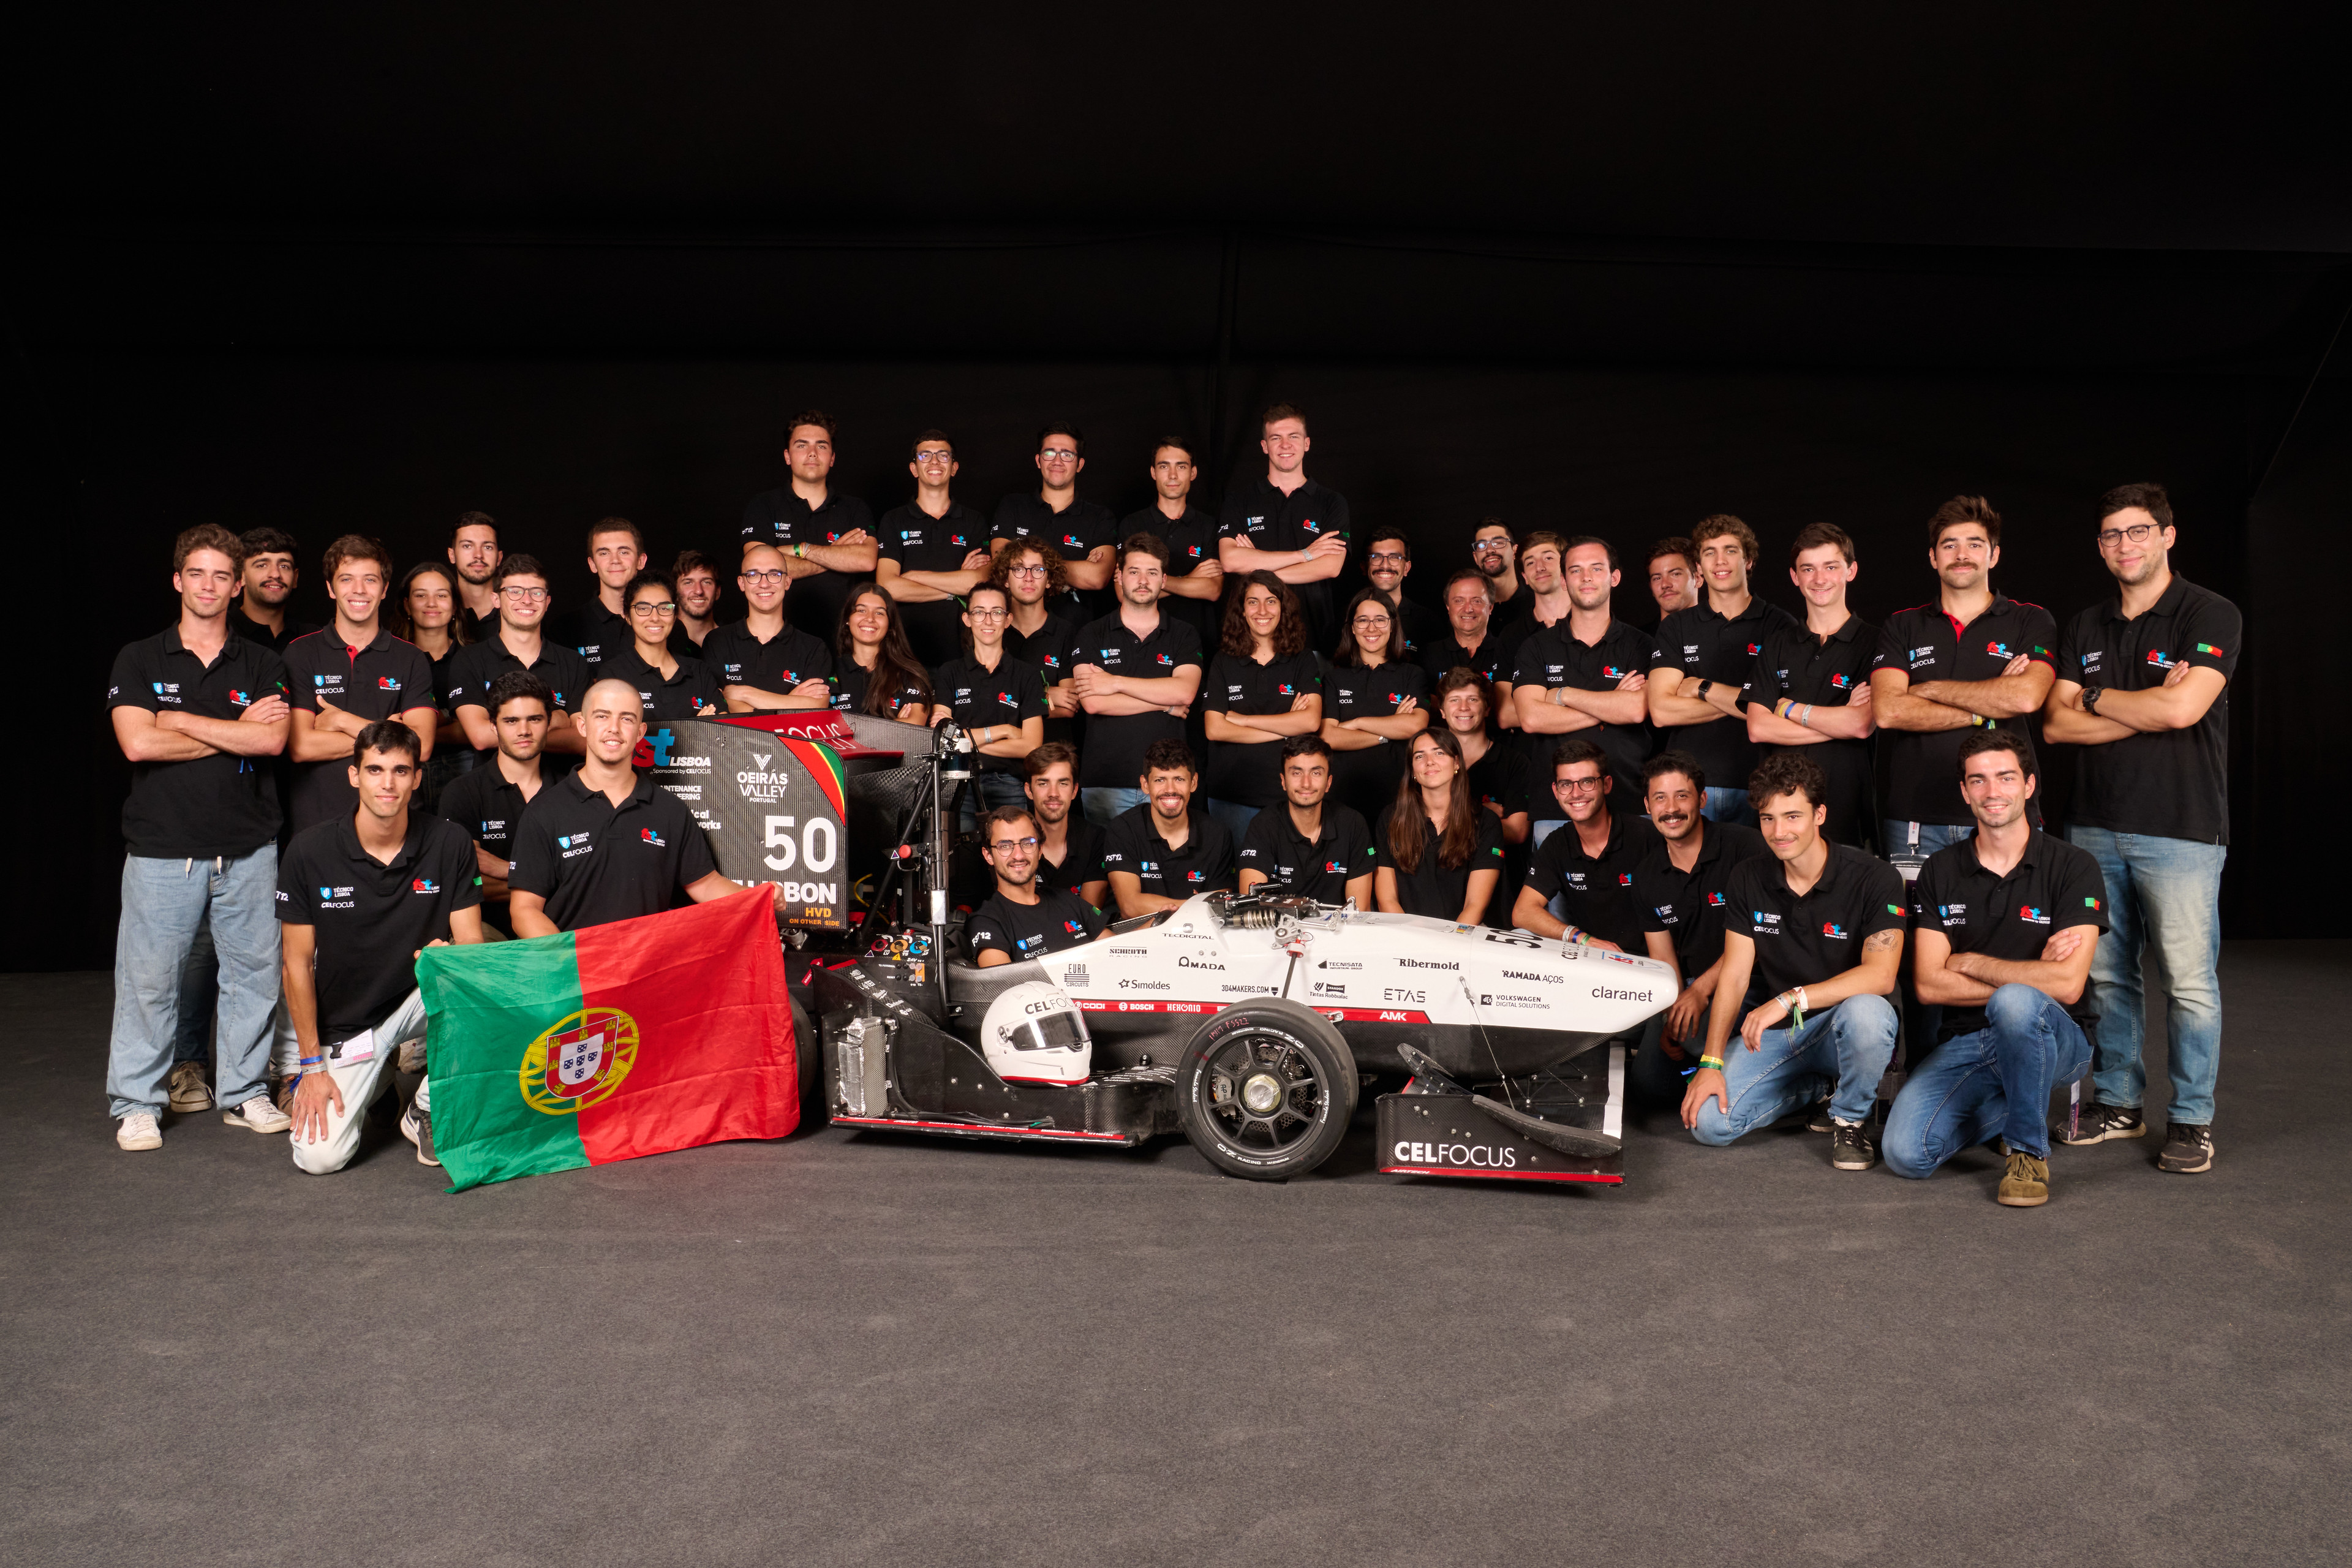
\includegraphics[clip, trim=4cm 18cm 4cm 19cm, width=1\textwidth]{Figures/20230817_11-40-48_7254_grobe.jpg}
	% }
	\caption[FST12 Team at Formula Student Germany Competition.]{FST12 Team at Formula Student Germany Competition, © FSG - Axel Grobe.}
	\label{fig:fst12_fsg}%chktex 24
\end{figure}
%%%%%%%%%%%%%%%%%%%%%%%%%%%%%%%%%%%%%%%%%%%%%%%%%%%%%%%%%%%%%%%%%%%%%%%%
% \section{Topic Overview}\label{section:intro_overview}
\section{Control Methods Overview}\label{section:control_methods_overview}

Through the years, several approaches have been proposed to control synchronous machines using a 2-level three-phase inverter. Regarding the control methods, several solutions have been presented in the literature with the most common being \gls{foc} and \gls{dtc}, with \gls{mpc}~\cite{Bianchi:control_review} being introduced more recently, seeking a compromise between the advantages of \gls{foc} and \gls{dtc}. Some approaches require a modulator such as \gls{svm}~\cite{Neacsu:SVM_intro:2001:IECON}, while others can directly output the semiconductor trigger signals~\cite{Vazquez:MPC_in_power_systems_review:2017:IEEE}.

The use of \gls{foc} and \gls{dtc} have dominated the market for many years due to their simple implementation, but each of them has downsides\@. \gls{foc} combined with current control PID is known for having a slow dynamic response when compared to \gls{dtc}, while in steady-state behavior and disturbance rejection, \gls{foc} shows better results~\cite{Merzoug:FOCvsDTC:2008,Korkmaz:FOCvsDTC:2013,Souad:FOCvsDTC:2008}. \gls{dtc} has a faster dynamic response, with the compromise of a higher torque ripple and a higher current \gls{thd}. \gls{mpc} has been proposed as a combination of the two, exhibiting a good dynamic response while being able to maintain low current and torque ripple. 
% Another advantage of \gls{dtc} strategy is that when using the standard implementation, the control method is based on the stator axis, thus it does not need rotor position sensors (albeit some implementations can benefit from it), thus having a lower cost and a simpler implementation.

Technical advances in the microprocessor industry have allowed the increasing use of \gls{mpc} in power converters and drives~\cite{Vazquez:MPC_in_power_systems_review:2017:IEEE}. This non-linear control scheme provides easy constraint integration while optimizing the control action in real time and is adaptable to different types of electric machines being controlled. The main downside of this strategy is the increased computational cost, which is offset by the decreased cost of computational power.

\gls{mpc} in power systems is usually divided in two categories: \gls{csmpc} and \gls{fsmpc}~\cite{Wang:MPC_in_Electrical_Machines_review:2017:IEEE}, depending on their output signals. The first type calculates the best possible voltage vector and then uses a modulator like \gls{svm} to compose it, while \gls{fsmpc} exploits the fact that a motor drive usually has a limited number of possible voltage combinations and thus predicts the currents for each of those vectors to evaluate the best option. The second approach usually doesn't need a modulator as it only considers the finite set of all possible converter states, although some variations have tried to increase the search space by introducing synthetic vectors that are created from a combination of the native ones. This technique of subdivision and refining vectors can be used to create a quasi-continuous set \gls{mpc}~\cite{Ma:MPC_Syntetic_vector:2014:IEEE}, which, when combined with reducing the search area to the most probable sector, can improve the torque and current ripple without a prohibitive increase in computational cost.
%%%%%%%%%%%%%%%%%%%%%%%%%%%%%%%%%%%%%%%%%%%%%%%%%%%%%%%%%%%%%%%%%%%%%%%%
\section{Thesis Objectives}\label{section:objectives}

This work targets to develop a nonlinear control strategy that allows the use of the existing high-efficiency inverter~\cite{Costa:MSc} with the commercial motors currently used by the team~\cite{amk:DD5-14-10-POW}. This control method must be able to achieve a faster dynamic response than the current inverter used by the team while maintaining or improving the same steady-state performance, and with a sampling time smaller than 20µs to allow a switching frequency of at least 50kHz.

While the improved control method will enhance the performance, not all the gains will come from that, but also the use of an inverter with \gls{sic} mosfets greatly increases the efficiency. The increase in switching frequency shall bring a reduction in the currents \gls{thd} resulting in further efficiency improvements. Lastly, the use of an inverter designed specifically for this motor will reduce the system mass, improving the power-to-weight ratio.

Summing up, this work aims to increase the dynamic response and the efficiency of the powertrain system using wide bandgap semiconductors and nonlinear control methods. This will be verified in simulations, and wherever possible with a prototype in a test bench, where the control method shall be compared with the \gls{oem} system. A revised version of the inverter will also be made, to improve the measurement robustness to \gls{emi} and to increase the maximum current limit of the semiconductors to match the motor's maximum current.


%%%%%%%%%%%%%%%%%%%%%%%%%%%%%%%%%%%%%%%%%%%%%%%%%%%%%%%%%%%%%%%%%%%%%%%%
\section{Thesis Outline}\label{section:outline}

Chapter 2 starts with an overview of formula student competitions, followed by an introduction to two-level inverters. Then a mathematical model for a \gls{pmsm} is developed, laying the ground for the proposal of the control methods The chapter ends with a brief review of the control methods state of the art.

In Chapter 3 the motor characterization methodology is defined and the current reference generation is presented. A load profile that represents the car is also defined, and the controllers studied in this work are proposed.

Chapter 4 presents simulations comparing the control methods and validation of the simulation model with experimental tests.

In Chapter 5 the conclusions are made, analyzing which objectives were fulfilled and proposing topics for future research. % file "Thesis_Introduction.tex"
% \cleardoublepage{} 
\newpage

%%%%%%%%%%%%%%%%%%%%%%%%%%%%%%%%%%%%%%%%%%%%%%%%%%%%%%%%%%%%%%%%%%%%%%%%
%                                                                      %
%     File: Thesis_Background.tex                                      %
%     Tex Master: Thesis.tex                                           %
%                                                                      %
%     Author: Israel Sother                                            %
%     Last modified: 27 May 2024                                       %
%                                                                      %
%%%%%%%%%%%%%%%%%%%%%%%%%%%%%%%%%%%%%%%%%%%%%%%%%%%%%%%%%%%%%%%%%%%%%%%%

\chapter{Theoretical Background and PMSM Model}
\label{chapter:background}%chktex 24

\minitoc% Creating a minitoc

This chapter covers some fundamentals used to develop this work. It starts with a brief overview of Formula Student competitions and the current powertrain system used by \gls{fst}. After this, it presents the basics on \gls{vsi} and modulation techniques before developing a mathematical model for the used motors and later converting it to discrete time. Lastly, a quick overview of the literature control methods is done before introducing the proposed strategy.
%%%%%%%%%%%%%%%%%%%%%%%%%%%%%%%%%%%%%%%%%%%%%%%%%%%%%%%%%%%%%%%%%%%%%%%%
%                                                                      %
%     File: FormulaStudent.tex           	                           %
%     Tex Master: Thesis.tex                                           %
%                                                                      %
%     Author: Israel Sother                                            %
%     Last modified: 27 May 2024                                       %
%                                                                      %
%%%%%%%%%%%%%%%%%%%%%%%%%%%%%%%%%%%%%%%%%%%%%%%%%%%%%%%%%%%%%%%%%%%%%%%%

\section{Formula Student}

In a formula student competition, two types of evaluation exist, the first category is comprised of static events where the design, cost, and business model of the prototype are analyzed. In the dynamic category, each prototype is evaluated through 5 different events: Skidpad, Acceleration, AutoX, Endurance, and Efficiency (evaluated in the Endurance track), as shown in figure \Cref{fig:fs_tracks}. To be able to compete in dynamic events each prototype needs to pass a series of safety and rule compliance inspections, a process which starts even before de competition with the documentation analysis and finishes with on-site scrutineering.

The Skidpad event is the least relevant for this study as it is designed to test the cornering ability of the vehicle. It is comprised of two circles of radius $9.125m$, where the vehicle performs an adaptation first lap and then the lap time is measured on the second lap, when the car is at steady state cornering. As it is a tight and steady course, the power consumption is low not reaching the regulations limit of $80kW$, thus the dynamic response and efficiency of the motors have almost no relevance to the performance. 

The acceleration event consists of a standing start $75m$ straight acceleration, with the maximum battery power limited to $80kw$, as it is for all Formula Student events. For this event, the key factors from a powertrain point of view are the torque dynamic response, and how efficiently the powertrain system can deliver power to the ground. 
\begin{figure}[!htb]
	\centering
	% \fbox{
	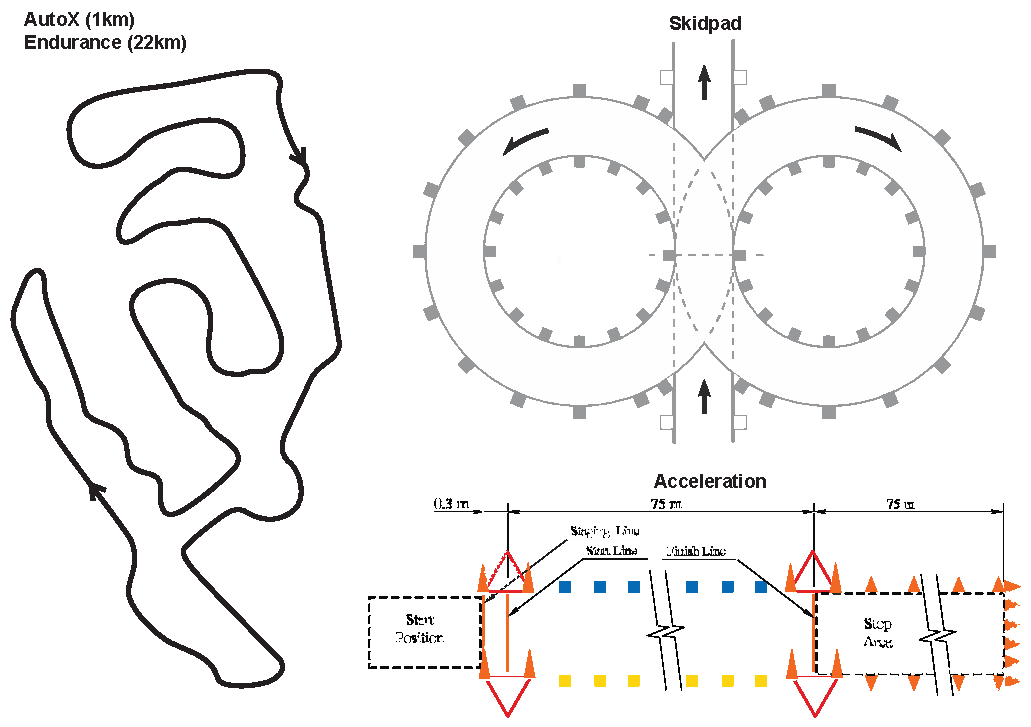
\includegraphics[width=0.8\textwidth]{Figures/Tracks.pdf}
	% }
	\caption[Formula Student Germany Tracks.]{Formula Student Germany Tracks, adapted from~\cite{FSG:rules:2023}.}
	\label{fig:fs_tracks} %chktex 24
\end{figure}
The AutoX is a $1km$ track with several corners and straights mixed. In this test, an increased dynamic response can delay the braking zone, and the efficiency allows it to reach higher velocities using the same amount of power. Lastly, the endurance event is similar to the AutoX, with enough laps to complete $22km$. In this event, although improved dynamics can be beneficial, efficiency is the key factor as it results in more available energy to complete the $22km$ track while also scoring points in the Efficiency category. 

For the autonomous part of the competition, there are very similar events, with the Skidpad and Acceleration being the same as in the manual mode. The driverless AutoX needs to be a little different, with a smaller distance for the \gls{asr} to be able to see the car throughout the entire track and press the emergency button if necessary. The Endurance event driverless analogous is the TrackDrive event, usually being on the same track as the AutoX, but with fixed 10 laps. Currently, the points performance in the driverless events is mostly dictated by how good the autonomous software is, but as the teams evolve, the cars will play a major role in the results, the same way as it is in the manual category.


Since the FST07, \gls{fst} has used AMK motors and inverters~\cite{amk:DD5-14-10-POW,amk:KW26-S5-FSE-4Q} (datasheets shown in \Cref{chapter:appendixDatasheets}), this set is a good solution for teams switching to a four-motor setup as it is already paired and has good documentation. However, as the team evolves, it is natural to look for improvements, and the AMK inverters were deemed one of the prototypes' current bottlenecks. The use of \gls{igbt} as the switching component, means that this inverter is capped in its switching frequency, using only 8kHz. This low switching frequency reduces powertrain efficiency and increases the set's weight. Another drawback of this solution is the control method as it uses a simple \gls{foc}, thus having a low dynamic response and further reducing efficiency by not using \gls{mtpa} strategies.
A brief outline of the current specification of \gls{fst}'s prototype is shown in \Cref{table:fst13_specs}.

\begin{table}[h]
	\centering
	\caption{FST13 Powertrain Specifications}
	\label{table:fst13_specs}%chktex 24
	\renewcommand{\arraystretch}{1.2} % more space between rows
	% \resizebox{0.85\textwidth}{!}{%
		\begin{tabular}{l l}
			\toprule
			% \rowcolor[HTML]{C0C0C0}
			\textbf{Parameter}                 & \textbf{Value} \\ \toprule
			Battery Voltage Min                & 420 V          \\ \hline
			Battery Voltage Maximum            & 609 V (limited at 600 V by regulations)          \\ \hline
			Battery Voltage Nominal            & 532 V          \\ \hline
			Maximum Power                      & 147 kW (limited at 80 kW by regulations)          \\ \hline
			Number of Motors                   & 4              \\ \hline
			% Motor types		                   & \gls{pmsm}\\ \hline
			% Motor Winding                      & Delta          \\ \hline
			% Motor magnet arrangement           & Spoke          \\ \hline
			Maximum Power per Motor            & 36.75 kW       \\ \hline
			Typical Average Power              & 30 kW          \\ \hline
			Maximum Average Power (1 min)      & 60 kW          \\ \hline
			Maximum Current DC                 & 160 A          \\ \hline
			Maximum motor current RMS (1,24s)  & 105 A          \\ \hline
			AMK Inverter Switching Frequency   & 8 kHz          \\ \hline
			Rotating magnetic field at Maximum Speed   & 1.6 kHz        \\ \hline
			Rated Motor Current                & 41 Arms        \\ \hline
			Rated Motor Voltage                & 350 V          \\ \hline
			% Average Current per phase          & 41             \\ \hline
			% RMS Current per phase              & 2              \\ \hline
			Maximum Speed                      & 20000 RPM      \\ \hline
			Motor Number of Poles              & 10             \\ \hline
			Quadrature Axis Inductance,        & 0.12 mH        \\ \hline
			Direct Axis Inductance             & 0.24 mH        \\ \hline
			Rotor time constant                & 0.01 s         \\ \hline
			Maximum Torque                     & 21 Nm          \\ \hline
			Torque constant                    & 0.26 Nm/Arms   \\ \hline
			Voltage constant                   & 18.8 V/kRPM    \\ \bottomrule
		\end{tabular}
	% }
\end{table}


%%%%%%%%%%%%%%%%%%%%%%%%%%%%%%%%%%%%%%%%%%%%%%%%%%%%%%%%%%%%%%%%%%%%%%%%
%                                                                      %
%     File: Inverter.tex		                                       %
%     Tex Master: Thesis.tex                                           %
%                                                                      %
%     Author: Israel Sother                                            %
%     Last modified: 27 May 2024                                       %
%                                                                      %
%%%%%%%%%%%%%%%%%%%%%%%%%%%%%%%%%%%%%%%%%%%%%%%%%%%%%%%%%%%%%%%%%%%%%%%%

\vfill
\section{Two Level Voltage Source Inverter}
\label{section:Two Level Voltage Source Inverter}%chktex 24
The usual hardware used to control synchronous machines is a 2-level Voltage Source Inverter. Such equipment is composed of six switches organized in three legs, where each pair of switches is connected to a motor terminal, as shown in \Cref{fig:inverter_and_motor_schematic}.

\begin{figure}[!htb]
	\centering
	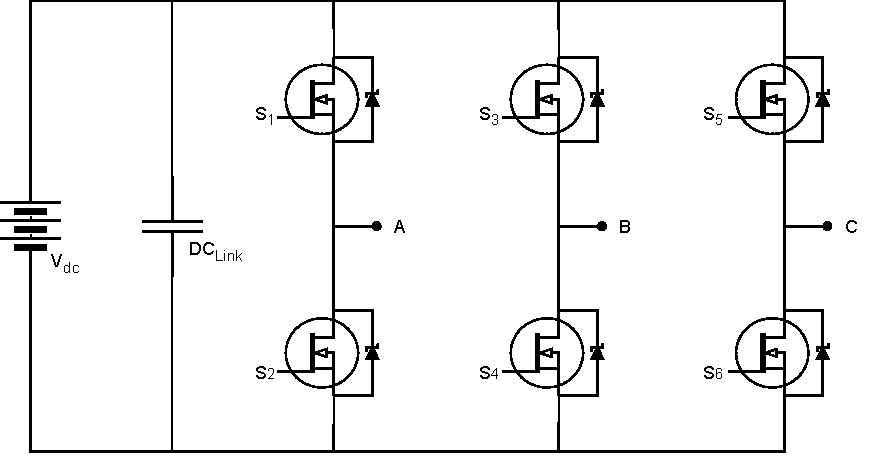
\includegraphics[width=0.7\textwidth]{Figures/Inverter.pdf}
	\caption[2-Level Voltage source Inverter arrangement.]{2-Level Voltage source Inverter arrangement.}
	\label{fig:inverter_and_motor_schematic}%chktex 24
\end{figure}

Usually, each switch in an inverter leg is operated with the inverse logic of the other switch in the leg, and this arrangement allows for 8 different switching combinations where 2 of them result in null voltages. That gives 7 possible voltage vectors, as detailed in \Cref{table:space_vector} and \Cref{fig:space_vector}. In \Cref{table:space_vector} the Vector column denotes the top switches states ($S_1$,$S_2$, and $S_3$), where a 1 means the top switch is the conducting state with the bottom switch is on a cut-off state and a 0 the opposite. The $\alpha$ and $\beta$ components which define the state space vectors are as defined by the Concordia transformation, shown in \Cref{eq:concordia}.

\begin{equation}
	\mathbf{Co} = \sqrt{\frac{2}{3}}
	\begin{bmatrix}
		1            & 0                   & \frac{1}{\sqrt{2}} \\
		-\frac{1}{2} & \frac{\sqrt{3}}{2}  & \frac{1}{\sqrt{2}} \\
		-\frac{1}{2} & -\frac{\sqrt{3}}{2} & \frac{1}{\sqrt{2}} \\
	\end{bmatrix}
	\label{eq:concordia}
\end{equation}

\begin{table}[h]
	\centering
	\caption{Switching combinations and space vectors for a 2-level three-phase inverter}
	\label{table:space_vector}%chktex 24
	\renewcommand{\arraystretch}{1.7} % more space between rows
	\resizebox{0.5\textwidth}{!}{%
		\begin{tabular}{|
				>{\columncolor[HTML]{E0E0E0}}c |
				>{\columncolor[HTML]{E0E0E0}}c |c|c|c|c|c|}
			\hline %chktex 44
			\cellcolor[HTML]{A0A0A0}\textbf{Switch State} &
			\cellcolor[HTML]{A0A0A0}\textbf{Vector}       &
			\cellcolor[HTML]{A0A0A0}\textbf{$V_{AB}$}     &
			\cellcolor[HTML]{A0A0A0}\textbf{$V_{BC}$}     &
			\cellcolor[HTML]{A0A0A0}\textbf{$V_{CA}$}	  &
			\cellcolor[HTML]{A0A0A0}\textbf{$V_{\alpha}$} &
			\cellcolor[HTML]{A0A0A0}\textbf{$V_{\beta}$}  \\ \hline %chktex 44
			0 & 000 & 0         & 0         & 0         & $0$                         & $0$                       \\ \hline %chktex 44
			1 & 001 & $V_{DC}$  & 0         & $-V_{DC}$ & $\sqrt{\frac{2}{3}}V_{DC}$  & $0$                       \\ \hline %chktex 44
			2 & 010 & $-V_{DC}$ & $V_{DC}$  & 0         & $\frac{1}{\sqrt{6}}V_{DC}$  & $\frac{1}{\sqrt{2}}V_{DC}$\\ \hline %chktex 44
			3 & 011 & 0         & $V_{DC}$  & $-V_{DC}$ & $-\frac{1}{\sqrt{6}}V_{DC}$ & $\frac{1}{\sqrt{2}}V_{DC}$\\ \hline %chktex 44
			4 & 100 & 0         & $-V_{DC}$ & $V_{DC}$  & $-\sqrt{\frac{2}{3}}V_{DC}$ & $0$                       \\ \hline %chktex 44
			5 & 101 & $V_{DC}$  & $-V_{DC}$ & 0         & $-\frac{1}{\sqrt{6}}V_{DC}$ & $\frac{1}{\sqrt{2}}V_{DC}$\\ \hline %chktex 44
			6 & 110 & $-V_{DC}$ & 0         & $V_{DC}$  & $\frac{1}{\sqrt{6}}V_{DC}$  & $\frac{1}{\sqrt{2}}V_{DC}$\\ \hline %chktex 44
			7 & 111 & 0         & 0         & 0         & $0$                         & $0$                       \\ \hline %chktex 44
		\end{tabular}%
	}
\end{table}


Despite the number of discrete voltage states, using some modulation techniques it is possible to synthesize a resultant vector if it is inside the attainable region denoted by the hexagon in \Cref{fig:space_vector}.

The current inverter used by \gls{fst} uses this structure, but the switches are silicon \glspl{igbt}, which when compared to \gls{sic} \glspl{mosfet} has a higher switching loss, leading to lower switching frequencies being used~\cite{Gurpinar:si_sic_gan_comparison:2016:IEEE}. The lower switching frequencies cause higher distortions in the current waveforms, decreasing motor efficiency. The lower switching frequency system also needs a higher capacitance on the DC Link, while the lower efficiency of silicon semiconductors requires a bigger heatsink, leading to a higher volume and mass inverter, decreasing the power density of the solution.

\subsection{Space Vector Modulation}
\label{subsection:Space Vector Modulation}%chktex 24

Several modulation techniques have been proposed in the literature like \gls{spwm}, \gls{she}~\cite{Asadzadeh:selective_harmonic_elimination:2019}, \gls{svm}~\cite{Neacsu:SVM_intro:2001:IECON}.
% , or \gls{svc}~\cite{An:space_vector_control:2016}. Some of these techniques are exclusive of multilevel inverters, like \gls{svc}~\cite{Rodriguez:svc_multilevel:2002}, while others also work for two-level inverters. 
The most common method of modulation in digital motor control is \gls{svm}, as it is a robust, easy-to-implement technique, and allows higher voltage ratio. 

% The figure "fig:space_vector" provides a visual representation of the space vector for a 2-level three-phase inverter. It shows the possible voltage states that can be applied to the motor. The phase voltages are represented in a 2D plane, with the maximum phase voltage shown by a circle. Any point within this circle is attainable without overmodulation or neutral point shift. The hexagon represents the maximum voltage that can be applied to the motor, and the vectors within the hexagon are the possible voltage states.
\Cref{fig:space_vector} shows a 2D representation of the space vector for a 2-level three-phase inverter. The basic voltage vectors (previously defined on \Cref{table:space_vector}) are shown pointing to the hexagon corners. 
% Note that they can only reach those voltages if modulation techniques that produce shifting in the neutral point (like third harmonic injection) are used.
 Connecting the basic vectors produces the hexagon of possible voltage states.

\begin{figure}[!htb]
	\centering
	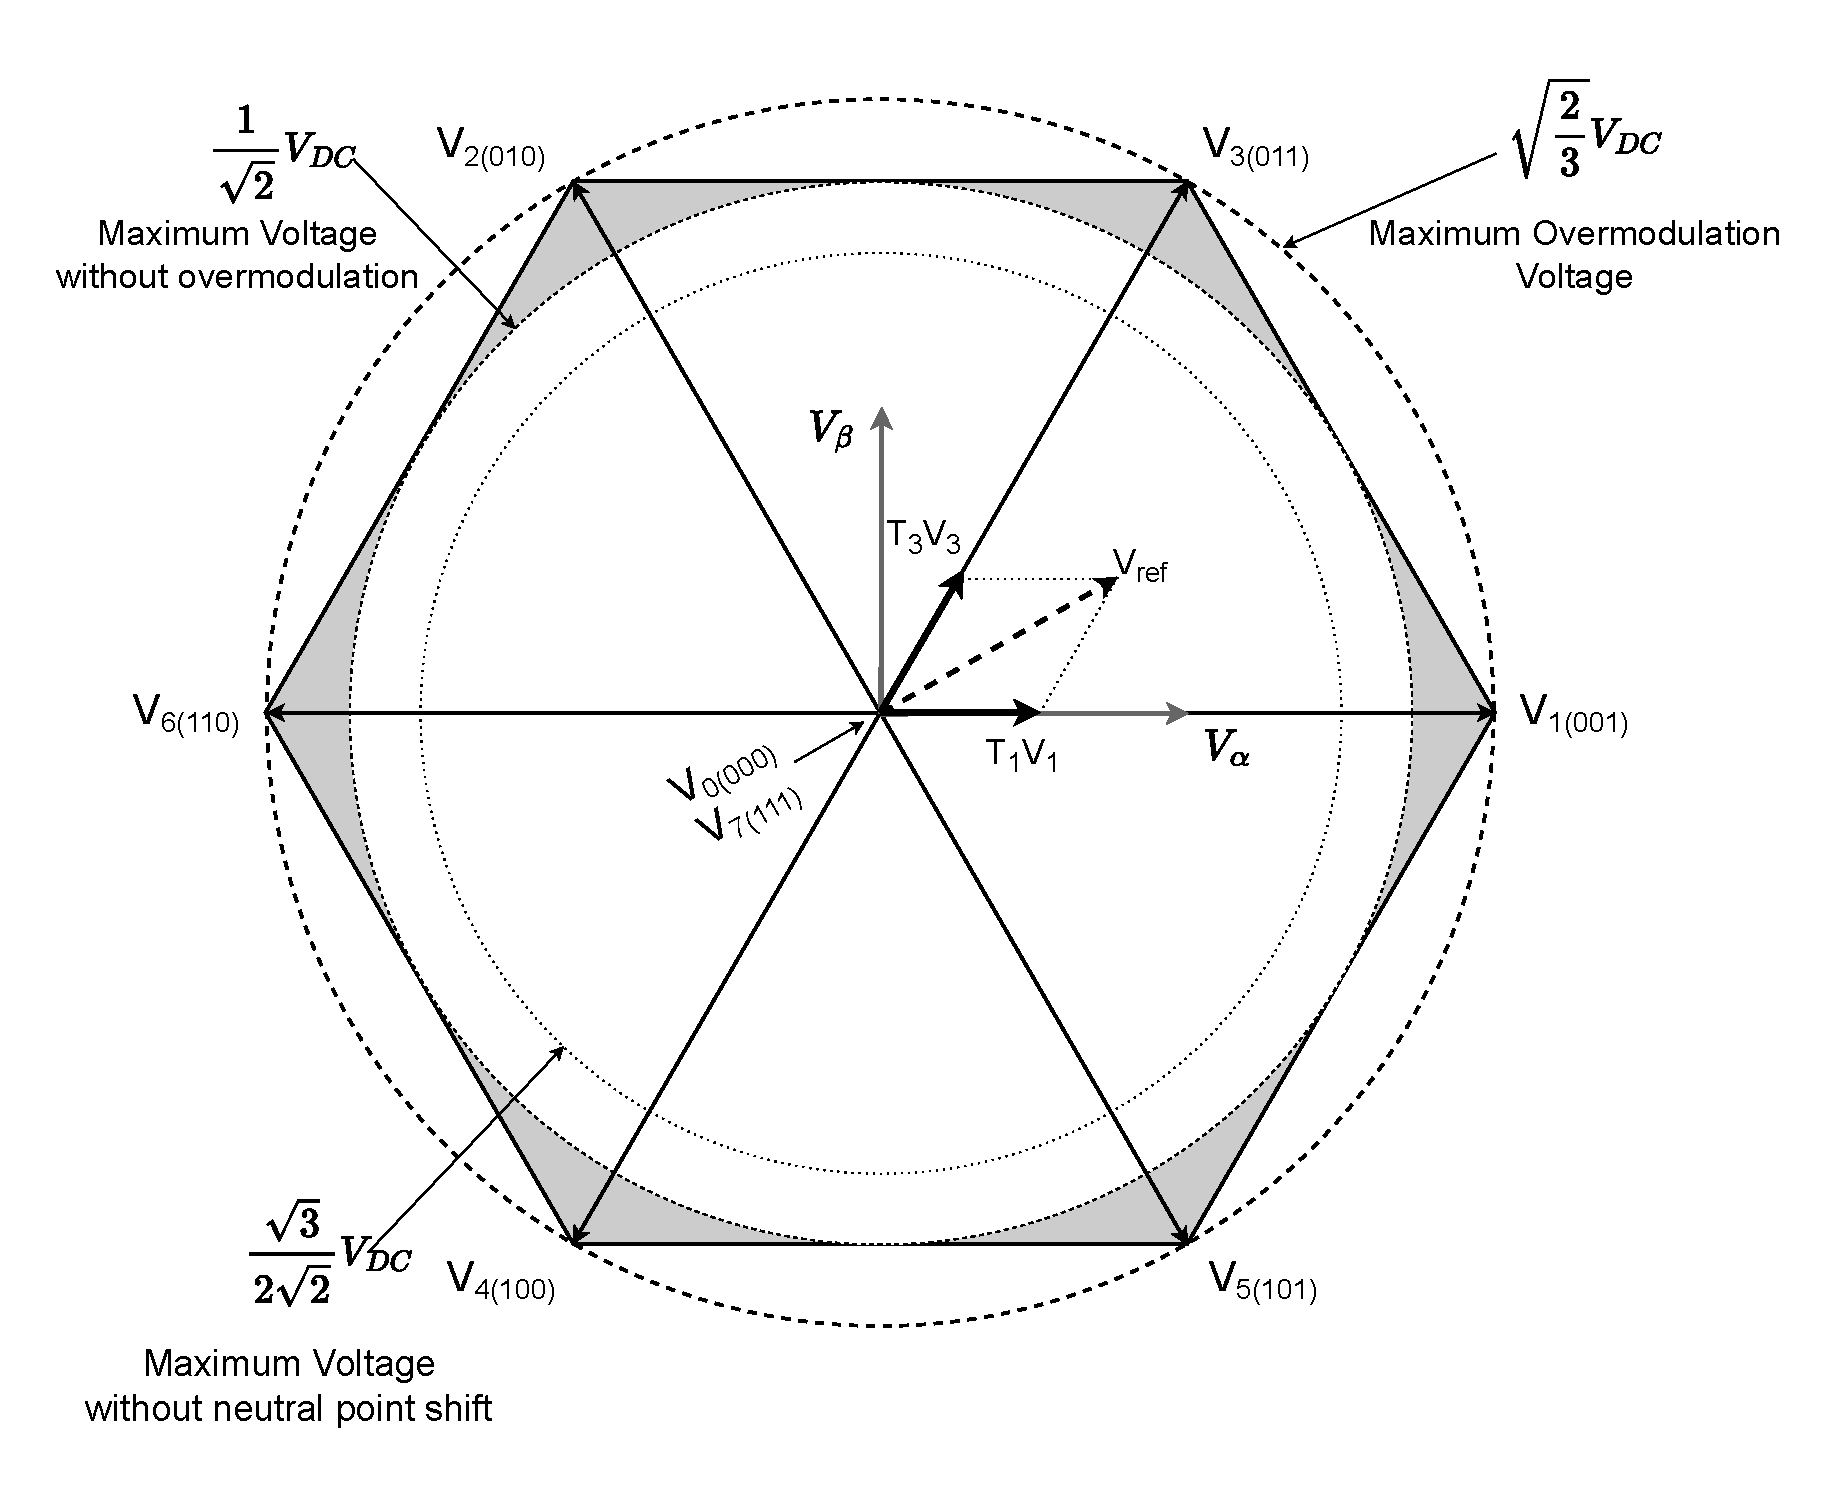
\includegraphics[width=0.8\textwidth]{Figures/Space_Vector_revised.pdf}
	\caption[Space vector for a 2-level three-phase inverter.]{Space vector for a 2-level three-phase inverter.}
	\label{fig:space_vector}%chktex 24
\end{figure}


Using \gls{svm} it is possible to modulate any vector inside the hexagon shown in \Cref{fig:space_vector}, but if a pure sinusoidal output is desired, the vectors should be constrained to the inscribed circle, that has a radius of $\frac{1}{\sqrt{2}} V_{DC}$. The reason behind this is to keep the reference vector locus inside the hexagon, avoiding distortions in the output. Note that although it is possible to generate waveforms with higher RMS value, it is not possible to modulate a peak higher than $\frac{1}{\sqrt{2}} V_{DC}$ for every vector angle. If a higher RMS value is requested the generated voltage will be saturated on the sides of the hexagon while near the corners it will achieve the requested value, thus those waveforms become more and more distorted as the amplitude approaches $\sqrt{\frac{2}{3}} V_{DC}$. To modulate a sinusoidal output the vector should develop a circular trajectory, but in the overmodulation region the voltage constrains it to the voltage hexagon, and thus the difference between the intended and the effectively applied vector increases.

To simplify the analysis of those vectors, a modulation index ($m$) is defined as shown in \Cref{eq:modulation_index}. The output is free of distortion if $m\le\frac{2}{\sqrt{3}}$, and increasing the modulation index further will result in diminishing returns in wave amplitude, while the output approaches a six-step commutation, greatly increasing the \gls{thd}~\cite{Microchip:Overmodulation:2023}. This area of operation is called overmodulation, and several approaches have been proposed~\cite{Briz:overmodulation_technique_field_weakening:2001,MehriziSani:advanced_modulation_techniques:2007} to minimize the distortions.
\begin{equation}
	m = \frac{2\sqrt{2}}{\sqrt{3}}\frac{\left|V{ref}\right|}{V_{DC}} \quad \quad m \;\in\; \left[0, \frac{4}{3}\right]
	\label{eq:modulation_index}
\end{equation}

To modulate a voltage vector that is not exactly one of the basic voltage vectors a modulation technique is needed. When using the \gls{svm} method to compose a given reference vector $V_{ref}$, the algorithm first detects the sector on which the reference vector lays. With the sector identified a ratio between the adjacent basic vectors and a null vector is selected so that the average vector is equal to the reference vector. This ratio is calculated as shown in \Cref{eq:svm_vref}.

For example, let's consider the reference vector shown in \Cref{fig:space_vector}. According to \gls{svm}, this vector can be modulated by using $V_1$ for half of the active time and $V_3$ for the other half of the active time. The active time refers to the duration when the vector amplitude is non-zero, while the null time refers to the duration when a null vector is used to reduce the output amplitude. This modulation can be expressed by \Cref{eq:svm_vref}, where $t_1+t_3$ represents the active time and $t_{n}$ represents the null time.

\begin{equation}
	V_{ref} = \frac{t_{n} V_{n} + t_1 V_1  + t_3 V_3}{h}
	\label{eq:svm_vref}
\end{equation}

%% epxplanation of the neutral point shift. it should follow the following equation: V_shift = K_{shift}*max(V_{AN},V_{BN},V_{CN) + (1-K_{shift})*min(V_{AN},V_{BN},V_{CN)


In the hardware implementation, the voltage reference is generated in the rotor reference frame (dq0) and then the inverse dq0 transformation is applied to obtain the phase voltages directly, without selecting a sector to know which vectors to use. These phase voltages are then divided by the DC link voltage to obtain the duty cycle of the switches. Note that this does not account though for the neutral point shift. This simplification results in the same switching times for the active vectors as the geometric approach of calculating which sector the reference vector is and then decomposing the reference vector in the two adjacent vectors. The null vector distribution between $V_0$ and $V_7$ will dictate the neutral point shifting method.

Several approaches have been proposed to accomplish this shift and they all rely on injecting a variable offset voltage on the neutral point that has a strong third harmonic component. Although a pure third harmonic sine wave can be used it is computationally expensive when compared with other methods such as top, mid, or bottom clamp. This technique of mid-clamp aims to center the neutral point between the DC link terminals, while the top clamp shifts the neutral point to the maximum voltage and the bottom clamp to the minimum voltage. The main advantage of a top or bottom clamp is the reduced number of switching events when compared with a mid-clamp. 

The chosen approach is defined by \Cref{eq:neutral_point_shift}, where $K_{shift}$ is the shift factor, and $V_{AN}$,$V_{BN}$, and $V_{CN}$ are the phase voltages referenced to a virtual neutral point that is the average of the phase voltages with respect to the DC link negative terminal. The value of $K_{shift}$ dictates the shift method used, when it is equal to 1 the top-clamp method is used, if it is 0.5 then the mid-clamp is used, and 0 results in the bottom-clamp method.~\citet{Microchip:ZSM_viewer:2023} has a visualization tool with the main methods shown. The calculated shift voltage is then summed to the desired phase voltages, and the modulation technique is applied as usual. In the implementation, this results in the \glspl{mosfet} duty cycle being shifted to center at the value of $K_{shift}$.

\begin{equation}
	V_{shift} = K_{shift} - K_{shift} \max \left(V_{AN},V_{BN},V_{CN}\right) - (1-K_{shift}) \min \left(V_{AN},V_{BN},V_{CN}\right)
	\label{eq:neutral_point_shift}
\end{equation}

%%%%%%%%%%%%%%%%%%%%%%%%%%%%%%%%%%%%%%%%%%%%%%%%%%%%%%%%%%%%%%%%%%%%%%%%
%                                                                      %
%     File: PMSM_model.tex                                             %
%     Tex Master: Thesis.tex                                           %
%                                                                      %
%     Author: Israel Sother                                            %
%     Last modified: 27 May 2024                                       %
%                                                                      %
%%%%%%%%%%%%%%%%%%%%%%%%%%%%%%%%%%%%%%%%%%%%%%%%%%%%%%%%%%%%%%%%%%%%%%%%
\section{PMSM model}\label{section:PMSM model}
As the proposed work is to improve the dynamic response and efficiency of the motor and motor drive currently used by \gls{fst}, it is necessary to first develop a model to represent this machine, a \gls{pmsm} with delta-arranged windings.

%%%%%%%%%%%%%%%%%%%%%%%%%%%%%%%%%%%%%%%%%%%%%%%%%%
\subsection{PMSM in ABC coordinates}
The stator voltages of the considered electrical machine can be given by \Cref{eq:flx_voltage_balance}, with a graphical representation in \Cref{fig:delta_model}.
\begin{equation}
	\begin{aligned}
		\begin{bmatrix}
			u_{AB} \\
			u_{BC} \\
			u_{CA} \\
		\end{bmatrix}
		=
		\begin{bmatrix}
			r_a & 0   & 0   \\
			0   & r_b & 0   \\
			0   & 0   & r_c \\
		\end{bmatrix}
		\begin{bmatrix}
			i_a \\
			i_b \\
			i_c \\
		\end{bmatrix}
		+
		\frac{d}{dt}
		\begin{bmatrix}
			\psi_a \\
			\psi_b \\
			\psi_c \\
		\end{bmatrix}
	\end{aligned}
	\label{eq:flx_voltage_balance}%chktex 24
\end{equation}

In this equation, $u_{xy}$ represents the measured voltage between terminal $x$ and $y$, $i_x$ is the current flowing on each phase, $r_x$ is the phase resistance, and $\psi_x$ is the flux linkage of each coil. Combining this in a matrix representation we can define the variables in \Cref{eq:variables_abc}.

\vspace{0.5cm}
\begin{subequations}
	\noindent\begin{minipage}{.38\linewidth}
		\begin{equation}
			\mathbf{R_{abc}} = \begin{bmatrix}
				r_a & 0   & 0   \\
				0   & r_b & 0   \\
				0   & 0   & r_c \\
			\end{bmatrix}
		\end{equation}
	\end{minipage}%
	\begin{minipage}{.3\linewidth}
		\begin{equation}
			\mathbf{i_{abc}} = \begin{bmatrix}
				i_a \\
				i_b \\
				i_c \\
			\end{bmatrix}
		\end{equation}
	\end{minipage}%
	\begin{minipage}{.3\linewidth}
		\begin{equation}
			\mathbf{u_{abc}} = \begin{bmatrix}
				u_{AB} \\
				u_{BC} \\
				u_{CA} \\
			\end{bmatrix}
		\end{equation}
	\end{minipage}%
	\label{eq:variables_abc}
\end{subequations}
\vspace{0.5cm}

Regarding the flux linkage, it can be defined as in \Cref{eq:flux_linkage}, where $\psi_{PM}$ is the permanent magnet flux linkage, and $\theta_e$ is the rotor electrical position. Additionally, the $L_{abc}$ matrix is the inductance matrix as later defined in \Cref{eq:phase_inductances}. With this definition, the \Cref{eq:flx_voltage_balance} can be expanded into \Cref{eq:voltage_balance}, where $E_x$ is the \gls{emf} as defined in \Cref{eq:back_emf}.

\begin{subequations}
	\noindent\begin{minipage}{.5\linewidth}
		\begin{equation}
			\pmb{\psi_{abc}} = \mathbf{L_{abc}i_{abc}} + \psi_{PM} \begin{bmatrix}
				\cos{\left(\theta_e\right)} \\
				\cos{\left(\theta_e - \frac{4\pi}{3}\right)} \\
				\cos{\left(\theta_e + \frac{4\pi}{3}\right)} \\
			\end{bmatrix}
			\label{eq:flux_linkage}
		\end{equation}
	\end{minipage}%
	\begin{minipage}{.49\linewidth}
		\begin{equation}
			\mathbf{E_{abc}} = 
			\begin{bmatrix}
				E_a \\
				E_b \\
				E_c \\
			\end{bmatrix} = \psi_{PM} \dot{\theta_e}
			 \begin{bmatrix}
				-\sin{\left(\theta_e\right)} \\
				-\sin{\left(\theta_e - \frac{4\pi}{3}\right)} \\
				-\sin{\left(\theta_e + \frac{4\pi}{3}\right)} \\
			\end{bmatrix}
			\label{eq:back_emf}
		\end{equation}
	\end{minipage}%
\end{subequations}



\begin{figure}[!htb]
	\centering
	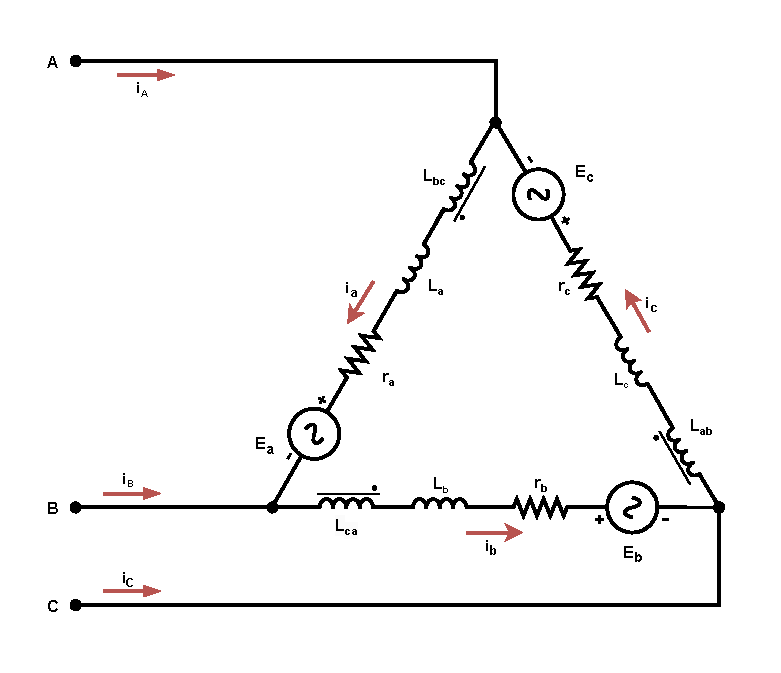
\includegraphics[width=0.6\textwidth]{Figures/Delta_model.pdf}
	\caption[Delta-wound \gls{pmsm}.]{Delta-wound \gls{pmsm}}
	\label{fig:delta_model}%chktex 24
\end{figure}
The expanded form results in~\Cref{eq:voltage_balance}.

\begin{equation}
	\mathbf{u_{abc}}
	=
	\mathbf{R_{abc}}
	\mathbf{i_{abc}}
	+
	% \begin{bmatrix}
	% 	L_{a}  & M_{ab} & M_{ac} \\
	% 	M_{ba} & L_{b}  & M_{bc} \\
	% 	M_{ca} & M_{cb} & L_{c}  \\
	% \end{bmatrix}
	\mathbf{L_{abc}}
	\frac{d\mathbf{i_{abc}}}{dt}
	+
	\frac{d\mathbf{L_{abc}}}{dt}  \mathbf{i_{abc}}
	+\mathbf{E_{abc}}
	\label{eq:voltage_balance}%chktex 24
\end{equation}


% \begin{equation}
% 	E_a + E_b + E_c + r(i_a + i_b + i_c) + (\mathbf{L} - 2\mathbf{M})\left( \frac{di_a}{dt} + \frac{di_b}{dt} + \frac{di_c}{dt}\right) = 0%chktex 7
% \end{equation}
Note that the inductances are not constant, but they change regarding the rotor electrical position $\theta_e$. This variation exists because the selected machine has a spoke magnet arrangement on the rotor, thus creating magnetic paths with different reluctances depending on the rotor angle. According to~\citet{Marques:Dinamica_das_maquinas_eletricas:2002}, this variation is a sum of even harmonics of a cosine function, but usually, it is enough to consider up to the second one, resulting in the inductance matrix shown in~\Cref{eq:phase_inductances}, where $L_{x_1}$,$L_{x_2}$,$M_{xy_1}$, and $M_{xy_2}$ are constants and define the coefficients for the self inductances and the mutual inductances.

\begin{equation}
	\mathbf{L_{abc}} =
	\begin{bmatrix}
		L_{a_1} + L_{a_2} \cos{ \left(2 \theta_e\right)}                    & M_{ab_1} + M_{ab_2} \cos{ \left(2 \theta_e + \frac{4\pi}{3}\right)} & M_{ac_1} + M_{ac_2} \cos{ \left(2 \theta_e - \frac{4\pi}{3}\right)} \\
		M_{ba_1} + M_{ba_2} \cos{ \left(2 \theta_e + \frac{4\pi}{3}\right)} & L_{b_1} + L_{b_2} \cos{ \left(2 \theta_e - \frac{4\pi}{3}\right)}   & M_{bc_1} + M_{bc_2} \cos{ \left(2 \theta_e\right)}                  \\
		M_{ca_1} + M_{ca_2} \cos{ \left(2 \theta_e - \frac{4\pi}{3}\right)} & M_{cb_1} + M_{cb_2} \cos{ \left(2 \theta_e\right)}                  & L_{c_1} + L_{c_2} \cos{ \left(2 \theta_e + \frac{4\pi}{3}\right)}   \\
	\end{bmatrix}
	\label{eq:phase_inductances}
\end{equation}

Is important to explain that the~\Cref{eq:phase_inductances} is derived assuming the 3 phases are separated by $120$ electrical degrees and that the windings have a sinusoidal magnetomotive force distribution.

For comprehensive understanding, the self inductances $L_x$ and the mutual inductances $L_{xy}$ depicted in \Cref{fig:delta_model} are as defined in \Cref{eq:induc_figure}.

\begin{subequations}
	\noindent
	\begin{minipage}{.485\linewidth}
		\begin{equation}
			L_{ab} = M_{ab_1} + M_{ab_2} \cos{ \left(2 \theta_e + \frac{4\pi}{3}\right)}
		\end{equation}
	\end{minipage}
	\begin{minipage}{.485\linewidth}
		\begin{equation}
			L_{ac} = M_{ac_1} + M_{ac_2} \cos{ \left(2 \theta_e - \frac{4\pi}{3}\right)}
		\end{equation}
	\end{minipage}
	\\
	\begin{minipage}{.485\linewidth}
		\begin{equation}
			L_{ba} = M_{ba_1} + M_{ba_2} \cos{ \left(2 \theta_e + \frac{4\pi}{3}\right)}
		\end{equation}
	\end{minipage}
	\begin{minipage}{.485\linewidth}
		\begin{equation}
			L_{bc} = M_{bc_1} + M_{bc_2} \cos{ \left(2 \theta_e\right)}
		\end{equation}
	\end{minipage}
	\\
	\begin{minipage}{.485\linewidth}
		\begin{equation}
			L_{ca} = M_{ca_1} + M_{ca_2} \cos{ \left(2 \theta_e - \frac{4\pi}{3}\right)}
		\end{equation}
	\end{minipage}
	\begin{minipage}{.485\linewidth}
		\begin{equation}
			L_{cb} = M_{cb_1} + M_{cb_2} \cos{ \left(2 \theta_e\right)}
		\end{equation}
	\end{minipage}
	\\
	\begin{minipage}{.485\linewidth}
		\begin{equation}
			L_{a} = L_{a_1} + L_{a_2} \cos{ \left(2 \theta_e\right)}
		\end{equation}
	\end{minipage}
	\begin{minipage}{.485\linewidth}
		\begin{equation}
			L_{b} = L_{b_1} + L_{b_2} \cos{ \left(2 \theta_e\right)}
		\end{equation}
	\end{minipage}
	\\
	\begin{minipage}{.95\linewidth}
		\begin{equation}
			L_{c} = L_{c_1} + L_{c_2} \cos{ \left(2 \theta_e\right)}
		\end{equation}
	\end{minipage}
	\label{eq:induc_figure}
\end{subequations}
%%%%%%%%%%%%%%%%%%%%%%%%%%%%%%%%%%%%%%%%%%%%%%%%%%
\subsection{dq0 Transformation}
\vfill
To simplify the mathematical models, some transformations were proposed. The most common is the dq0 transformation, which is a combination of the Concordia and the Blondel-Park transformations. The Concordia transformation converts a three-phase system into an equivalent two-phase system, where the two phases are orthogonal to each other, they are called $\alpha$ and $\beta$ components. This transformation has two main versions, the amplitude invariant, and the power invariant. The power invariant version, initially presented in \Cref{eq:concordia}, is shown again in \Cref{eq:concordia1} for easier reference.

The Blondel-Park transformation is a rotating referential transformation, where the referential is synchronous with the rotor position. The transformation matrix is shown in \Cref{eq:blondel_park}. Note that throughout this work the alignment of the transformation is always the $d$ component with the phase $a$. The dq0 transformation is a combination of the Concordia transformation, and the Park referential change, it produces a biphasic equivalent system with a synchronous rotating referential. The transformation matrix is shown in \Cref{eq:dq0}.

\begin{subequations}
	% \noindent
	\begin{minipage}{.4\linewidth}
		\begin{equation}
			\mathbf{Co} = \sqrt{\frac{2}{3}}
			\begin{bmatrix}
				1            & 0                   & \frac{1}{\sqrt{2}} \\
				-\frac{1}{2} & \frac{\sqrt{3}}{2}  & \frac{1}{\sqrt{2}} \\
				-\frac{1}{2} & -\frac{\sqrt{3}}{2} & \frac{1}{\sqrt{2}} \\
			\end{bmatrix}
			\label{eq:concordia1}
		\end{equation}
	\end{minipage}
	\begin{minipage}{.485\linewidth}
		\begin{equation}
			\mathbf{Bl}_{(\theta_e)} = 	\begin{bmatrix}
				\cos{\left(\theta_e\right)} & -\sin{\left(\theta_e\right)} & 0 \\
				\sin{\left(\theta_e\right)} & \cos{\left(\theta_e\right)}  & 0 \\
				0                           & 0                            & 1 \\
			\end{bmatrix}
			\label{eq:blondel_park}
		\end{equation}
	\end{minipage}
\end{subequations}
\begin{equation}
	\mathbf{T}_{(\theta_e)} = \mathbf{Co} \; \mathbf{Bl}_{(\theta_e)}
	=
	\sqrt{\frac{2}{3}}
	\begin{bmatrix}
		\cos{\left(\theta_e\right)}                & -\sin{\left(\theta_e\right)}                & \frac{1}{\sqrt{2}} \\
		\cos{\left(\theta_e-\frac{2\pi}{3}\right)} & -\sin{\left(\theta_e-\frac{2\pi}{3}\right)} & \frac{1}{\sqrt{2}} \\
		\cos{\left(\theta_e-\frac{4\pi}{3}\right)} & -\sin{\left(\theta_e-\frac{4\pi}{3}\right)} & \frac{1}{\sqrt{2}} \\
	\end{bmatrix}
	\label{eq:dq0}
\end{equation}

The power invariant transformation has the advantage of being an orthogonal matrix, thus $\mathbf{T}^{-1} = \mathbf{T}^T$.\\
If the amplitude invariant form is used, as in \Cref{eq:blondel_park_amplitude_invariant}, then orthogonality is lost.

\begin{subequations}
	% \begin{minipage}{.45\linewidth}
	\begin{equation}
		\mathbf{T}^*_{(\theta_e)} =
		\begin{bmatrix}
			\cos{\left(\theta_e\right)}                & -\sin{\left(\theta_e\right)}                & 1 \\
			\cos{\left(\theta_e-\frac{2\pi}{3}\right)} & -\sin{\left(\theta_e-\frac{2\pi}{3}\right)} & 1 \\
			\cos{\left(\theta_e-\frac{4\pi}{3}\right)} & -\sin{\left(\theta_e-\frac{4\pi}{3}\right)} & 1 \\
		\end{bmatrix}
	\end{equation}
	% \end{minipage}%
	% \begin{minipage}{.55\linewidth}
	\begin{equation}
		{\mathbf{T}^*_{(\theta_e)}}^{-1} = \frac{2}{3}
		\begin{bmatrix}
			\cos{\left(\theta_e\right)}  & \cos{\left(\theta_e-\frac{2\pi}{3}\right)}  & \cos{\left(\theta_e-\frac{4\pi}{3}\right)}  \\
			-\sin{\left(\theta_e\right)} & -\sin{\left(\theta_e-\frac{2\pi}{3}\right)} & -\sin{\left(\theta_e-\frac{4\pi}{3}\right)} \\
			\frac{1}{2}                  & \frac{1}{2}                                 & \frac{1}{2}                                 \\
		\end{bmatrix}
	\end{equation}
	\label{eq:blondel_park_amplitude_invariant}%chktex 24
	% \end{minipage}%
\end{subequations}

Applying the power invariant transformation to the abc variables results in \Cref{eq:variables_dq0}.

\begin{subequations}
	\noindent
	\begin{minipage}{.5\linewidth}
		\begin{equation}
			\mathbf{R_{dq0}} = \mathbf{T}^T_{(\theta_e)} \mathbf{R_{abc}}\mathbf{T}_{(\theta_e)}
		\end{equation}
	\end{minipage}%
	\begin{minipage}{.5\linewidth}
		\begin{equation}
			\mathbf{L_{dq0}} = \mathbf{T}^T_{(\theta_e)} \mathbf{L_{abc}}\mathbf{T}_{(\theta_e)}
		\end{equation}
	\end{minipage}%
	\\
	\begin{minipage}{.33\linewidth}
		\begin{equation}
			\mathbf{i_{abc}} = \mathbf{T}_{(\theta_e)} \mathbf{i_{dq0}}
		\end{equation}
	\end{minipage}%
	\begin{minipage}{.33\linewidth}
		\begin{equation}
			\mathbf{u_{dq0}} = \mathbf{T}^T_{(\theta_e)} \mathbf{u_{abc}}
		\end{equation}
	\end{minipage}%
	\begin{minipage}{.33\linewidth}
		\begin{equation}
			\pmb{\psi_{abc}} = \mathbf{T}_{(\theta_e)} \pmb{\psi_{dq0}}
		\end{equation}
	\end{minipage}%
	\label{eq:variables_dq0}
\end{subequations}

% Or, using the amplitude invariant form:

% \begin{subequations}
% 	\noindent
% 	\begin{minipage}{.5\linewidth}
% 		\begin{equation}
% 			\mathbf{R_{dq0}} = {\mathbf{T}^*_{(\theta_e)}}^{-1} \mathbf{R_{abc}}\mathbf{T}^*_{(\theta_e)}
% 		\end{equation}
% 	\end{minipage}%
% 	\begin{minipage}{.5\linewidth}
% 		\begin{equation}
% 			\mathbf{L_{dq0}} ={\mathbf{T}^*_{(\theta_e)}}^{-1} \mathbf{L_{abc}}\mathbf{T}^*_{(\theta_e)}
% 		\end{equation}
% 	\end{minipage}%
% 	\\
% 	\begin{minipage}{.33\linewidth}
% 		\begin{equation}
% 			\mathbf{i_{abc}} = \mathbf{T}^*_{(\theta_e)} \mathbf{i_{dq0}}
% 		\end{equation}
% 	\end{minipage}%
% 	\begin{minipage}{.33\linewidth}
% 		\begin{equation}
% 			\mathbf{u_{dq0}} = {\mathbf{T}^*_{(\theta_e)}}^{-1} \mathbf{u_{abc}}
% 		\end{equation}
% 	\end{minipage}%
% 	\begin{minipage}{.33\linewidth}
% 		\begin{equation}
% 			\pmb{\psi_{abc}} = \mathbf{T}^*_{(\theta_e)} \pmb{\psi_{dq0}}
% 		\end{equation}
% 	\end{minipage}%
% 	\label{eq:variables_dq0_amplitude}
% \end{subequations}


%%%%%%%%%%%%%%%%%%%%%%%%%%%%%%%%%%%%%%%%%%%%%%%%%%
\subsection{PMSM in dq0 coordinates}

Assuming the three phases are well balanced and using the dq0 transformation (power invariant form) to transform the model into a two-phase system with a rotating referential, new resistance and inductance matrices can be computed to this new referential. The new matrices are shown in \Cref{eq:inductance_and_resistance_dqd0}, with the subscripts $_d$, $_q$,$_0$, denoting the direct axis, the quadrature axis, and the zero-sequence axis, respectively. The transformation of the matrices is detailed in~\citet{Marques:Dinamica_das_maquinas_eletricas:2002}.

\vspace{0.5cm}
\begin{subequations}
	\begin{minipage}{.53\linewidth}
		\begin{equation}
            \mathbf{R_{dq0}} =
            \begin{bmatrix}
                r_a & 0   & 0   \\
                0   & r_b & 0   \\
                0   & 0   & r_c \\
            \end{bmatrix} =
            \begin{bmatrix}
                r & 0 & 0 \\
                0 & r & 0 \\
                0 & 0 & r \\
            \end{bmatrix}
		\end{equation}
	\end{minipage}%
	\begin{minipage}{.43\linewidth}
		\begin{equation}
            \mathbf{L_{dq0}} =
            \begin{bmatrix}
                L_d & 0   & 0   \\
                0   & L_q & 0   \\
                0   & 0   & L_0 \\
            \end{bmatrix}
		\end{equation}
    \end{minipage}
	\label{eq:inductance_and_resistance_dqd0}
\end{subequations}
\vspace{0.5cm}

Starting with \Cref{eq:flx_voltage_balance} and replacing the currents and flux linkages by their dq0 components results in \Cref{eq:voltage_balance_dq0_intermediary}.

\begin{equation}
	\begin{aligned}
		\mathbf{u_{abc}}
		=
		\mathbf{R_{abc}}
		\mathbf{T}_{(\theta_e)} \mathbf{i_{dq0}}
		+
		\frac{d\left(\mathbf{T}_{(\theta_e)} \pmb{\psi_{dq0}}\right)}{dt}
		\\
		=
		\mathbf{R_{abc}}
		\mathbf{T}_{(\theta_e)} \mathbf{i_{dq0}}
		+\dot{\theta}_e\frac{d\mathbf{T}_{(\theta_e)}}{d\theta_e}\pmb{\psi_{dq0}}
		+\mathbf{T}_{(\theta_e)}\frac{d \pmb{\psi_{dq0}}}{dt}
	\end{aligned}
	\label{eq:voltage_balance_dq0_intermediary}
\end{equation}
Replacing $\dot{\theta}_e$ with $\omega_e$, and multiplying $\mathbf{T}^T_{(\theta_e)}$ to the left yields \Cref{eq:voltage_balance_dq0_intermediary2}.
\begin{equation}
	\begin{aligned}
		\mathbf{u_{dq0}}
		=
		\mathbf{R_{dq0}}\mathbf{i_{dq0}}
		+\mathbf{T}^T_{(\theta_e)}\omega_e\frac{d\mathbf{T}_{(\theta_e)}}{d\theta_e}\pmb{\psi_{dq0}}
		+\mathbf{T}^T_{(\theta_e)}\mathbf{T}_{(\theta_e)}\frac{d \pmb{\psi_{dq0}}}{dt}
	\end{aligned}
	\label{eq:voltage_balance_dq0_intermediary2}
\end{equation}
As the transformation matrix is orthogonal, it can be further simplified, as in \Cref{eq:voltage_balance_dq0_intermediary3}.
\begin{equation}
	\begin{aligned}
		\mathbf{u_{dq0}}
		=
		\mathbf{R_{dq0}}\mathbf{i_{dq0}}
		+\omega_e\mathbf{T}^T_{(\theta_e)}\frac{d\mathbf{T}_{(\theta_e)}}{d\theta_e}\pmb{\psi_{dq0}}
		+\frac{d \pmb{\psi_{dq0}}}{dt}
	\end{aligned}
	\label{eq:voltage_balance_dq0_intermediary3}
\end{equation}
Lastly, calculate the derivative of the transformation matrix, as in \Cref{eq:transformation_derivative_intermediary,eq:transformation_derivative}.
\begin{equation}
	\label{eq:transformation_derivative_intermediary}
	\mathbf{T}^T_{(\theta_e)}\frac{d\mathbf{T}_{(\theta_e)}}{d\theta_e} = 	\frac{2}{3}
	\begin{bmatrix}
		\cos{\left(\theta_e\right)}  & \cos{\left(\theta_e-\frac{2\pi}{3}\right)}  & \cos{\left(\theta_e-\frac{4\pi}{3}\right)}  \\
		-\sin{\left(\theta_e\right)} & -\sin{\left(\theta_e-\frac{2\pi}{3}\right)} & -\sin{\left(\theta_e-\frac{4\pi}{3}\right)} \\
		\frac{1}{\sqrt{2}}           & \frac{1}{\sqrt{2}}                          & \frac{1}{\sqrt{2}}                          \\
	\end{bmatrix}
	\begin{bmatrix}
		-\sin{\left(\theta_e\right)}                & -\cos{\left(\theta_e\right)}                & 0 \\
		-\sin{\left(\theta_e-\frac{2\pi}{3}\right)} & -\cos{\left(\theta_e-\frac{2\pi}{3}\right)} & 0 \\
		-\sin{\left(\theta_e-\frac{4\pi}{3}\right)} & -\cos{\left(\theta_e-\frac{4\pi}{3}\right)} & 0 \\
	\end{bmatrix}
\end{equation}
\begin{equation}
	\label{eq:transformation_derivative}
	\mathbf{T}^T_{(\theta_e)}\frac{d\mathbf{T}_{(\theta_e)}}{d\theta_e} =
	\begin{bmatrix}
		0 & -1 & 0 \\
		1 & 0  & 0 \\
		0 & 0  & 0 \\
	\end{bmatrix}
\end{equation}
Thus, the \gls{pmsm} model in the dq0 frame is presented in \Cref{eq:flx_voltage_balance_dq0}. This approach can be used for the amplitude invariant transformation and will result in the same form of equation (\Cref{chapter:appendixdq0_amplitude}), but the equation will be scaled by a factor of $\sqrt{\frac{3}{2}}$ in the d and q axis, while the zero axis can give different results.
\begin{equation}
	\mathbf{u_{dq0}}
	=
	\mathbf{R_{dq0}}\mathbf{i_{dq0}}
	+\omega_e	\begin{bmatrix}
		0 & -1 & 0 \\
		1 & 0  & 0 \\
		0 & 0  & 0 \\
	\end{bmatrix}
	\pmb{\psi_{dq0}}
	+\frac{d \pmb{\psi_{dq0}}}{dt}
	\label{eq:flx_voltage_balance_dq0}
\end{equation}

Is worth noticing that because this is a delta wound machine, the sum of the phase currents is not necessarily zero, and as such, it is mathematically possible to have a circulating current through the phases~\cite{Pramod:circulating_currents_delta_winding:2023}, thus the zero-sequence component is not directly zero as in a Y wound device. For such currents to exist, an external exciting winding, a relevant non-considered inductance harmonic, or an imbalance through the phases is necessary. Even when those currents are present, they are usually dependent on the rotor position, and cannot be controlled with the standard 3-terminal connection,
% \textbf{REFERENCE HERE}. Some studies have shown that the zero-sequence current component is relatively small compared to the direct and quadrature ones \textbf{REFERENCE HERE}, and
thus for the sake of simplicity, they are discarded throughout this work, which gives \Cref{eq:motor_blondel_park}.
\begin{subequations}
	\begin{equation}
		u_d = r i_d+\frac{d\psi_d}{dt} - \omega_e \psi_q\\
		\label{eq:motor_blondel_park_d} %chktex 24
	\end{equation}
	\begin{equation}
		u_q = r i_q+\frac{d\psi_q}{dt} + \omega_e \psi_d\\
		\label{eq:motor_blondel_park_q} %chktex 24
	\end{equation}
	\begin{equation}
		T_e = p(\psi_d i_q - \psi_q i_d)\\
	\end{equation}
	\begin{equation}
		\frac{d\omega_e}{dt} = \frac{T_e-T_{load} - T_{loss}}{J}\\
	\end{equation}
	\begin{equation}
		\frac{d\theta_e}{dt} = \omega_e
	\end{equation}
	\label{eq:motor_blondel_park} %chktex 24
\end{subequations}

Here $\omega_e$ is the rotor electrical rotational velocity, $p$ is the number of pole pairs, $J$ is the rotor rotational inertia, while $T_e$ is the electromagnetic torque, $T_{load}$ is the reaction torque of the load attached to the motor, and $T_{loss}$ is a torque equivalent to the losses on the motor (such as iron or friction losses).



If $\psi$ is assumed to be of form $\psi = i_x L_x + \psi_{PM_x}$ where the inductance only varies with the current and the permanent magnets flux ($\psi_{PM_x}$) is defined as constant and affecting only the direct axis ($\psi_{PM_q} = 0$), \Cref{eq:motor_blondel_park_d,eq:motor_blondel_park_q} result in \Cref{eq:motor_with_inductances}.

\begin{subequations}
	\begin{equation}
		% \left\{
		% \begin{aligned}
		u_d = r i_d+\frac{d i_d}{dt}\left(L_d + i_d\frac{d L_d}{di_d}\right) - \omega_e L_q i_q                \\
	\end{equation}
	\begin{equation}
		u_q = r i_q+ \frac{d i_q}{dt} \left(L_q + i_q\frac{d L_q}{di_q}\right) + \omega_e (L_d i_d +\psi_{PM}) \\
		% T_e  = p\, i_q(( L_d - L_q)i_d + \psi_{PM})                                                              \\ %= p( (L_d i_d + \psi_{PM}) i_q - L_q i_q i_d)\\
		% \frac{d\omega_e}{dt} = \frac{T_e-T_{load} - T_{loss}}{J}                                                 \\
		% \frac{d\theta_e}{dt} = \omega_e
		% \end{aligned}
		% \right.
	\end{equation}
	\label{eq:motor_with_inductances}
\end{subequations}
Note that in \Cref{eq:motor_with_inductances} the cross-magnetization effect is not accounted for, but the saturation is included in the inductance variation~\cite{Ohm:saturation_inductance:2000}.
If the inductance derivative is small when compared with the other terms, it can be further simplified to \Cref{eq:motor_with_inductances_no_derivative}.
\begin{subequations}
	\begin{equation}
		% \left\{
		% \begin{aligned}
		u_d = r i_d+L_d\frac{d i_d}{dt} - \omega_e L_q i_q              \\
	\end{equation}
	\begin{equation}
		u_q = r i_q+L_q\frac{d i_q}{dt} + \omega_e (L_d i_d +\psi_{PM})
	\end{equation}
	\begin{equation}
		T_e  = p\, i_q(( L_d - L_q)i_d + \psi_{PM})                       \\ %= p( (L_d i_d + \psi_{PM}) i_q - L_q i_q i_d)
	\end{equation}
	\begin{equation}
		\frac{d\omega_e}{dt} = \frac{T_e-T_{load} - T_{loss}}{J}
	\end{equation}
	\begin{equation}
		\frac{d\theta_e}{dt} = \omega_e
		% \end{aligned}
		% \right.
	\end{equation}
	\label{eq:motor_with_inductances_no_derivative}
\end{subequations}

Lastly, for the sake of completeness, if the amplitude invariant dq0 transformation is used, the currents need to be multiplied by a factor of $\sqrt{\frac{3}{2}}$ in the torque equation to have a power conservative output, resulting in~\Cref{eq:torque_amplitude_invariant}. The $\sqrt{\frac{2}{3}}$ next to the $\psi_{PM}$ is just a reminder that the flux linkage value has a different value depending on the dq0 transformation used.
\begin{equation}
	T_e  = 1.5p\, i_q(( L_d - L_q)i_d + \sqrt{\frac{2}{3}}\psi_{PM})
	\label{eq:torque_amplitude_invariant}
\end{equation}
%%%%%%%%%%%%%%%%%%%%%%%%%%%%%%%%%%%%%%%%%%%%%%%%
\subsection{Discretization of the PMSM model}
\vfill
An approximation of the differential equations is needed to discretize the equations to be able to use the model in a discrete time control system. Two usual solutions are the Backward and the Forward Euler methods. Although simpler to compute, the Forward Euler method is prone to instabilities especially in fast systems such as power converters, in contrast with the Backward alternative that is unconditionally stable. Due to this consideration, the Euler Backward technique will be prioritized.

From \Cref{eq:motor_with_inductances_no_derivative}, knowing that the currents and voltages vary with time and that the inductances are dependent on the currents the derivatives are isolated, as shown in \Cref{eq:model_derivatives}.
\begin{subequations}
	\begin{equation}
	\frac{d i_d}{dt} = \frac{u_d - r i_d + \omega_e L_q i_q}{L_d}
	\end{equation}
	\begin{equation}
	\frac{d i_q}{dt} = \frac{u_q - r i_q - \omega_e (L_d i_d +\psi_{PM})}{L_q}
	\end{equation}
	\begin{equation}
		T_e  = p\, i_q(( L_d - L_q)i_d + \psi_{PM})
	\end{equation}
	\begin{equation}
	\frac{d\omega_e}{dt} = \frac{T_e-T_{load} - T_{loss}}{J}
	\end{equation}
	\begin{equation}
	\frac{d\theta_e}{dt} = \omega_e
	\end{equation}
	\label{eq:model_derivatives}
\end{subequations}
 
Then it is possible to discretize the system with $h$ as the sampling time, and $t = kh$. As the Backward Euler method is desired, the derivatives are approximated by \Cref{eq:backward_euler_example}, resulting in \Cref{eq:motor_with_inductances_discrete}

\begin{equation}
    \frac{dy}{dt} = \frac{y(k+1) - y(k)}{h}
	\label{eq:backward_euler_example}
\end{equation}

\begin{equation}
	\left\{
	\begin{aligned}
		\frac{i_{d(k+1)}-i_{d(k)}}{h} = \frac{u_{d(k+1)} -r i_{d(k+1)} +\omega_{e(k+1)} L_{q(i_q(k+1))} i_{q(k+1)}}{L_{d(i_d(k+1))}}               \\
		\frac{i_{q(k+1)}-i_{q(k)}}{h} = \frac{u_{q(k+1)} -r i_{q(k+1)} - \omega_{e(k+1)} (L_{d(i_d(k+1))} i_{d(k+1)} +\psi_{PM})}{L_{q(i_q(k+1))}} \\
		T_{e(k+1)}  = p\, i_{q(k+1)}(( L_{d(i_d(k+1))} - L_{q(i_q(k+1))})i_{d(k+1)} + \psi_{PM})                                                   \\
		\frac{\omega_{e(k+1)} - \omega_{e(k)}}{h} = \frac{T_{e(k+1)}-T_{load(k+1)} - T_{loss(k+1)}}{J}                                             \\
		\frac{\theta_{e(k+1)} - \theta_{e(k)}}{h} = \omega_{e(k+1)}
	\end{aligned}
	\right.
	\label{eq:motor_with_inductances_discrete}
\end{equation}

This set of equations has an algebraic loop, where the currents in $k+1$ depend on the value of $\omega_{(k+1)}$, that depends on the value of $T_{e(k+1)}$ that is defined by the currents in $k+1$. The same thing happens with the inductances, as they depend on the currents, but the currents define the value of inductance. Those problems are solved by first assuming that the inductance change due to the current change in a time step is small enough so that the inductances can be calculated using the previous time step currents ($ L_{x(i_x(k+1))} \approx L_{x(i_x(k))} $). Similarly, the rotor speed is assumed to vary little between iterations, so that $\omega_{(k+1)} \approx \omega_{(k)}$.

With those considerations, and rearranging the equations, the system can be solved iteratively, as shown in \Cref{eq:motor_backward_euler_matrix}.

% \begin{equation}
% 	\left\{
% 	\begin{aligned}
% 		i_{d(k+1)}
% 		= \frac{h(u_{d(k+1)} +\omega_{e(k)} L_{q(i_q(k))} i_{q(k+1)}) + i_{d(k)}L_{d(i_d(k))}}{hr  + L_{d(i_d(k))}}                        \\
% 		i_{q(k+1)} =
% 		\frac{h\left(u_{q(k+1)} - \omega_{e(k)} (L_{d(i_d(k))} i_{d(k+1)} +\psi_{PM})\right) + i_{q(k)} L_{q(i_q(k))}}{hr + L_{q(i_q(k))}} \\
% 		T_{e(k+1)}  = p\, i_{q(k+1)}(( L_{d(i_d(k+1))} - L_{q(i_q(k+1))})i_{d(k+1)} + \psi_{PM})                                           \\
% 		\omega_{e(k+1)} = \omega_{e(k)} + h\left(\frac{T_{e(k+1)}-T_{load(k+1)} - T_{loss(k+1)}}{J}\right)                                 \\
% 		\theta_{e(k+1)} = \theta_{e(k)} + h\omega_{e(k+1)}
% 	\end{aligned}
% 	\right.
% 	\label{eq:motor_backward_euler}
% \end{equation}

% Or, in matrix form, as shown in \Cref{eq:motor_backward_euler_matrix}.
\begin{subequations}
	\begin{equation}
		\begin{aligned}
			\begin{bmatrix}
				i_{d(k+1)} \\
				i_{q(k+1)} \\
			\end{bmatrix}
			=
			\begin{bmatrix}
				1                                                    & -h\frac{\omega_{e(k)}L_{q(i_q(k))}}{hr+L_{d(i_d(k))}} \\
				h\frac{\omega_{e(k)}L_{d(i_d(k))}}{hr+L_{q(i_q(k))}} & 1                                                     \\
			\end{bmatrix}^{-1} \\
			\left(
			\begin{bmatrix}
					\frac{L_{d(i_d(k))}}{hr+L_{d(i_d(k))}} & 0                                      \\
					0                                      & \frac{L_{q(i_q(k))}}{hr+L_{q(i_q(k))}} \\
				\end{bmatrix}
			\begin{bmatrix}
					i_{d(k)} \\
					i_{q(k)} \\
				\end{bmatrix}
			+
			\begin{bmatrix}
					\frac{h}{hr+L_{d(i_d(k))}} & 0                          \\
					0                          & \frac{h}{hr+L_{q(i_q(k))}} \\
				\end{bmatrix}
			\begin{bmatrix}
					u_{d(k+1)} \\
					u_{q(k+1)} \\
				\end{bmatrix}
			+
			\begin{bmatrix}
					0                                                 \\
					-h\frac{\omega_{e(k)}\psi_{PM}}{hr+L_{q(i_q(k))}} \\
				\end{bmatrix}
			\right)
		\end{aligned}
	\end{equation}

	\begin{equation}
		T_{e(k+1)}  = p\, i_{q(k+1)}((L_{d(i_d(k+1))} - L_{q(i_q(k+1))})i_{d(k+1)} + \psi_{PM})
	\end{equation}

	\begin{equation}
		\begin{aligned}
			\begin{bmatrix}
				\omega_{e(k+1)} \\
				\theta_{e(k+1)}
			\end{bmatrix}
			=
			\begin{bmatrix}
				1 & 0 \\
				h & 1
			\end{bmatrix}
			\begin{bmatrix}
				\omega_{e(k)} \\
				\theta_{e(k)}
			\end{bmatrix}
			+
			\frac{T_{e(k+1)}-T_{load(k+1)} - T_{loss(k+1)}}{J}
			\begin{bmatrix}
				h \\
				h^2
			\end{bmatrix}
		\end{aligned}
	\end{equation}
	\label{eq:motor_backward_euler_matrix}
\end{subequations}
%%%%%%%%%%%%%%%%%%%%%%%%%%%%%%%%%%%%%%%%%%%%%%%%%%%%%%%%%%%%%%%%%%%%%%%%
%                                                                      %
%     File: Control_methods_overview.tex                               %
%     Tex Master: Thesis.tex                                           %
%                                                                      %
%     Author: Israel Sother                                            %
%     Last modified: 27 May 2024                                       %
%                                                                      %
%%%%%%%%%%%%%%%%%%%%%%%%%%%%%%%%%%%%%%%%%%%%%%%%%%%%%%%%%%%%%%%%%%%%%%%%
\vfill
\section{Control Methods State of the Art}\label{section:control_methods}
The quest for higher efficiency and performance has pushed the development in the field of control of electrical machines, and even though several advances have been made, the main strategies in the market are still the \gls{foc} with PID current control, and \gls{dtc}. While robust and well-known, these methods cannot explore the full performance envelope of the controlled machines, and the development of more complex machines with increased dynamic response and efficiency has pushed for new control strategies. In this context, the use of \gls{mpc} has grown as a good alternative as it explicitly considers the system dynamics and constraints.

\subsection{Field Oriented Control}

For many years field oriented control has been one of the cornerstones of electrical machine control due to its simplicity and easy implementation~\cite{Doncker:Universal_FOC:1994}. This technique is based on the Blondel Park transformation, where it converts the currents and voltages from a stationary ABC reference frame into a rotating referential dq0. This allows the individual control of the motor magnetic flux and torque, which are proportional to $i_d$ and $i_q$ respectively. These currents usually are controlled using two separated PIDs, where the quadrature current reference comes from the desired motor torque and the direct current comes from the field weakening strategy. The PIDs compare the references with the measured values and output a voltage to be applied in each axis, voltages that are passed to a modulator (usually \gls{svm}) to calculate the duty cycle of each \gls{mosfet} and generate the control signals. An example of such a system is shown in \Cref{fig:example_PID}.
\begin{figure}[!htb]
	\centering
	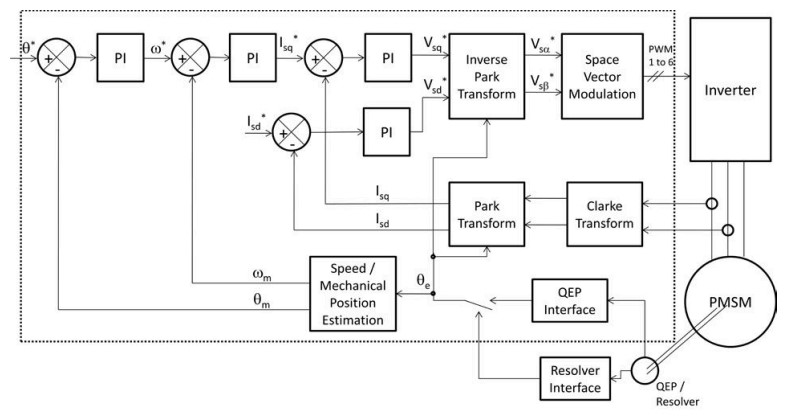
\includegraphics[width=1\textwidth]{Figures/foc_texas_instruments.jpg}
	\caption[Field Oriented Control - from Texas Instruments~\cite{TI:FOC_TMS320F2837:2016}.]{Field Oriented Control - from Texas Instruments~\cite{TI:FOC_TMS320F2837:2016}.}
	\label{fig:example_PID} %chktex 24
\end{figure}

While simple and robust, this technique heavily depends on the rotor position which is not always available, thus often needing some form of estimation to work correctly. Despite this limitation, \gls{foc} is a versatile method, being suitable not only for \gls{pmsm}, but also for induction motors, reluctance machines, among others~\cite{Hoang:FOC_vs_DTC_induction:1999,Matsuo:FOC_reluctance:1993}. One of the great advantages of \gls{foc} is that it produces a smooth operation in the full range of the motor, with low current distortions and reduced torque ripple~\cite{Adhavan:FOC_fuzzy:2011}.



\subsection{Direct Torque Control}
The principal rivel of \gls{foc} is \gls{dtc}, it shows better dynamic response with simpler implementation and less dependency on machine characterization~\cite{Hoang:FOC_vs_DTC_induction:1999}. Popularized by its use on induction machines, this method usually operates at the abc reference frame, calculating the flux based on the voltage and current vectors as in \Cref{eq:dtc_flux}, where $V_s$ is the stator voltage vector, $I_s$ is the stator current vector, $R_s$ is the stator resistance matrix, and $\psi_r$ is the rotor magnetic flux vector. Using this information, the torque can be calculated as in \Cref{eq:dtc_tq}, where $p$ is the number of pole pairs. When using an induction machine it is not necessary to have a rotor position, but on \gls{pmsm} this becomes a necessity as in \gls{foc}.

\begin{subequations}
	\begin{minipage}{.45\linewidth}
        \begin{equation}
            \psi_s = \int (V_s -R_s I_s)dt + \psi_r
            \label{eq:dtc_flux}
        \end{equation}
    \end{minipage}
    \begin{minipage}{.45\linewidth}
        \begin{equation}
            T_e = p(\psi_s I_s)
            \label{eq:dtc_tq}
        \end{equation}
    \end{minipage}
\end{subequations}

With these states calculated, a simple hysteresis band is applied to each, torque and flux, to select one of the 8 possible voltage vectors. This selection is done based on a lookup table that depending on the output of both hysteresis controllers, chooses the vector that pushes the torque and flux towards its references. This table can be generated using several strategies with different resultant dynamics~\cite{Buja:DTC_lookup_strategies:1997,Nasr:DTC_PMSM_improvement:2022}. The general schema of the \gls{dtc} is shown in \Cref{fig:example_DTC}.
\begin{figure}[!htb]
	\centering
	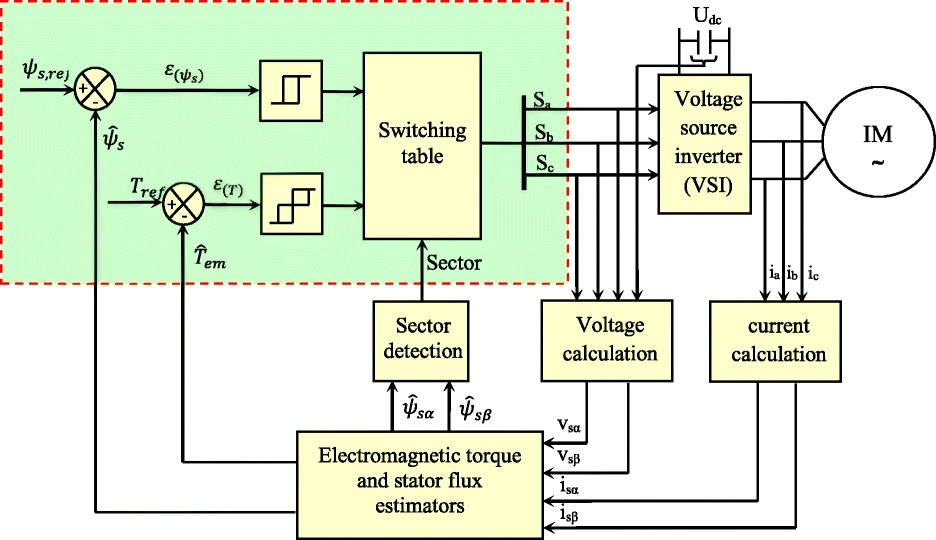
\includegraphics[width=0.8\textwidth]{Figures/dtc_schema.jpg}
	\caption[Direct Torque Control - from~\citet{Quanjli:DTC_schema:2019}.]{Direct Torque Control - from~\citet{Quanjli:DTC_schema:2019}.}
	\label{fig:example_DTC} %chktex 24
\end{figure}
Note that the nature of only switching vectors when the hysteresis is surpassed results in a variable switching frequency as opposed to \gls{foc} that has a fixed switching frequency. Another feature of the \gls{dtc} is that it does not need any modulators, as it directly chooses the voltage vector to be applied.

 \gls{dtc} is a very accessible method, with simpler implementation than \gls{foc} a faster dynamic response and low sensitivity to motor parameters, but it falls short in steady state operation with torque and current ripple often bigger than its rival \gls{foc}~\cite{Zhong:DTC_pmsm_dynamics:1997,Niu:DTC_vs_other_DTC_vs_FOC:2016}.



\subsection{Model Predictive Control}
With the increase in computational power, the \gls{mpc} has gained space among the machine controllers as it handles multivariable non-linear cases, is easy to integrate constraints, and has a great dynamic response and integrates constraint managing~\cite{Vazquez:MPC_uses:2014}. The model predictive controller's basic idea is to use a mathematical model of the controlled system to test several control actions and make a prediction about the system response. This prediction is then evaluated by a cost function that can include some soft constraints and the control action with the smaller cost is chosen as optimal.~\citet{Vazquez:MPC_in_power_systems_review:2017:IEEE} classifies the topologies typically used in power converters and drives into continuous set, and finite set, based on the process used to find the optimal control. 

Continuous set is very similar to predictive controllers used on other control fields, it computes a continuous control signal and uses a modulator to generate these voltage vectors. This topology comes with the advantage of fixed switching frequency at the cost of harder implementation and processing power requirements, as it needs an optimization solver. The finite set topology explores the limited control options of power converters to simplify the optimization process. This topology tests a set of the possible control vectors (this set can contain all or part of the possible vectors), and evaluates each of the vectors based on the predictions. While simpler to formulate, this method results in the chosen vector being applied to the full switching period, which results in a higher ripple when compared with a strategy that uses a modulator at the same control frequency. Another property of this strategy is the variable switching frequency, as the same vector can be chosen consecutively. 

To reduce the problem of applying the vector for the full timestep, a subset of finite set topology was presented. It adds time as part of the equation by computing the optimal switching sequence instead of the optimal switching vector, similar to a modulator~\cite{Vazquez:MPC_in_power_systems_review:2017:IEEE}. This allows the controller to choose a set of vectors to be switched in a given sequence with a duration also chosen by the controller.

When applied to \gls{pmsm} the predictive controllers are commonly designed with the dq0 model \Cref{eq:motor_with_inductances_no_derivative}~\cite{Sun:MPC_deadbeat_PMSM:2021}, and may track the currents or the torque to a given reference. The current tracking computational cost tends to be lower as the current optimization can be done offline while tracking torque makes online parameter estimation easier. If the topology is chosen to be continuous, a solver needs to be designed, one of the approaches is to expand the model and cost function into Taylor series approximations, and then use the derivative of the cost function to create a control law~\cite{Errouissi:MPC_taylor_series:2012}. 
% The main issues with developing an \gls{mpc} are to correctly model the system, proper cost function design, and manage computational cost to enable implementation, % file "Thesis_Ba©ckground.tex"
% \cleardoublepage{} ©
\newpage

%%%%%%%%%%%%%%%%%%%%%%%%%%%%%%%%%%%%%%%%%%%%%%%%%%%%%%%%%%%%%%%%%%%%%%%%
%                                                                      %
%     File: Thesis_Implementation.tex                                  %
%     Tex Master: Thesis.tex                                           %
%                                                                      %
%     Author: Israel Sother                                            %
%     Last modified: 27 May 2024                                       %
%                                                                      %
%%%%%%%%%%%%%%%%%%%%%%%%%%%%%%%%%%%%%%%%%%%%%%%%%%%%%%%%%%%%%%%%%%%%%%%%

\chapter{Machine Characterization and Control Methodology}
\label{chapter:implementation} %chktex 24
\minitoc% Creating a minitoc

%%%%%%%%%%%%%%%%%%%%%%%%%%%%%%%%%%%%%%%%%%%%%%%%%%%%%%%%%%%%%%%%%%%%%%%%
%                                                                      %
%     File: Motor_characteriztion.tex                                  %
%     Tex Master: Thesis.tex                                           %
%                                                                      %
%     Author: Israel Sother                                            %
%     Last modified: 27 May 2024                                       %
%                                                                      %
%%%%%%%%%%%%%%%%%%%%%%%%%%%%%%%%%%%%%%%%%%%%%%%%%%%%%%%%%%%%%%%%%%%%%%%%
\section{Motor characterization}
\label{section:motor_characterization}
\vfill

Although AMK has provided the motor datasheet (shown in \Cref{chapter:appendixDatasheets}) with the key parameters on it, it is important to verify how well they track the real values, and how they change regarding the motor operation. The datasheet values are linear approximations of the magnetic circuit on the motor, and as such do not accurately represent the machine at high current operating points. To account for the saturation effect, a variable inductance approach will be used~\cite{Wijenayake:saturation_model:1997,Stumberger:saturation_model:2003}, where the inductance of each axis will be a function of the current on the respective axis. 
% As explained in \Cref{chapter:background}, this would result in an algebraic loop, so an approximation is used, where the inductances at $k$ will be a function of the currents at $k-1$.

% To characterize the motor a few variables need to be defined, they are:
% \begin{itemize}
% 	\item Magnet flux linkage ($\psi_{PM}$)
% 	\item Phase resistance ($r$)
% 	\item Direct and Quadrature inductances ($L_d$ and $L_q$)
% \end{itemize}
\subsection{Phase resistance}
Assuming the machine is well balanced, the phase resistance will be equal to $\frac{3}{2}$ of the terminal resistance. Although a multimeter can be used, it will give poor precision, as the resistance is very low, so it's better to use a milliohmmeter or even better a micro-ohmmeter. A good practice would be to evaluate the parameters at different temperatures, especially the resistance, but that would require some specific hardware that is currently not available for this work.

The used device was a \textit{UNI-T UT620A Micro-ohmmeter}, that has a resolution of $10\mu \Omega$ with an accuracy of $\pm (0.25\% + 25\mu \Omega)$. The measurements were taken on the terminal wires at room temperature and with the kelvin probe, resulting in $142.89 \pm 0.06 m\Omega$. This value is close to the datasheet one of $135 m\Omega$, and the difference is probably due to the wire terminals. The resultant phase resistance ($r$) is $214.335 \pm 0.091 m\Omega$.
\subsection{Flux Linkage}
The magnet flux linkage can be measured by externally rotating the rotor and measuring the generated \gls{emf}. From \Cref{eq:motor_with_inductances}, if the terminal wires are disconnected from everything, the current will be constantly zero, thus the measured voltage will be only a result of the flux linkage and the rotor velocity as shown in \Cref{eq:flux_measuring}.

\begin{subequations}
	\begin{equation}
		u_d = r_d \cancelto{0}{i_d}+\cancelto{0}{\frac{d i_d}{dt}}\left(L_d + \cancelto{0}{i_d}\frac{d L_d}{di_d}\right) - \omega_e L_q \cancelto{0}{i_q} = 0                \\
	\end{equation}
	\begin{equation}
		u_q = r_q \cancelto{0}{i_q}+ \cancelto{0}{\frac{d i_q}{dt}} \left(L_q + \cancelto{0}{i_q}\frac{d L_q}{di_q}\right) + \omega_e (L_d \cancelto{0}{i_d} +\psi_{PM})  = \omega_e \psi_{PM}\\
	\end{equation}
	\label{eq:flux_measuring}
\end{subequations}

Using an external device, the rotor was kept at a constant speed that was measured by the digital encoder in the AMK motor, while an oscilloscope (\textit{Promax OD-571}) was connected to two terminal wires. The oscilloscope on the used settings has an accuracy of $\pm(3\% + 0.2508 V)$. An example of the output is shown in \Cref{fig:flux_measure_oscilloscope}.

% \begin{figure}[!htb]
% 	\centering
% 	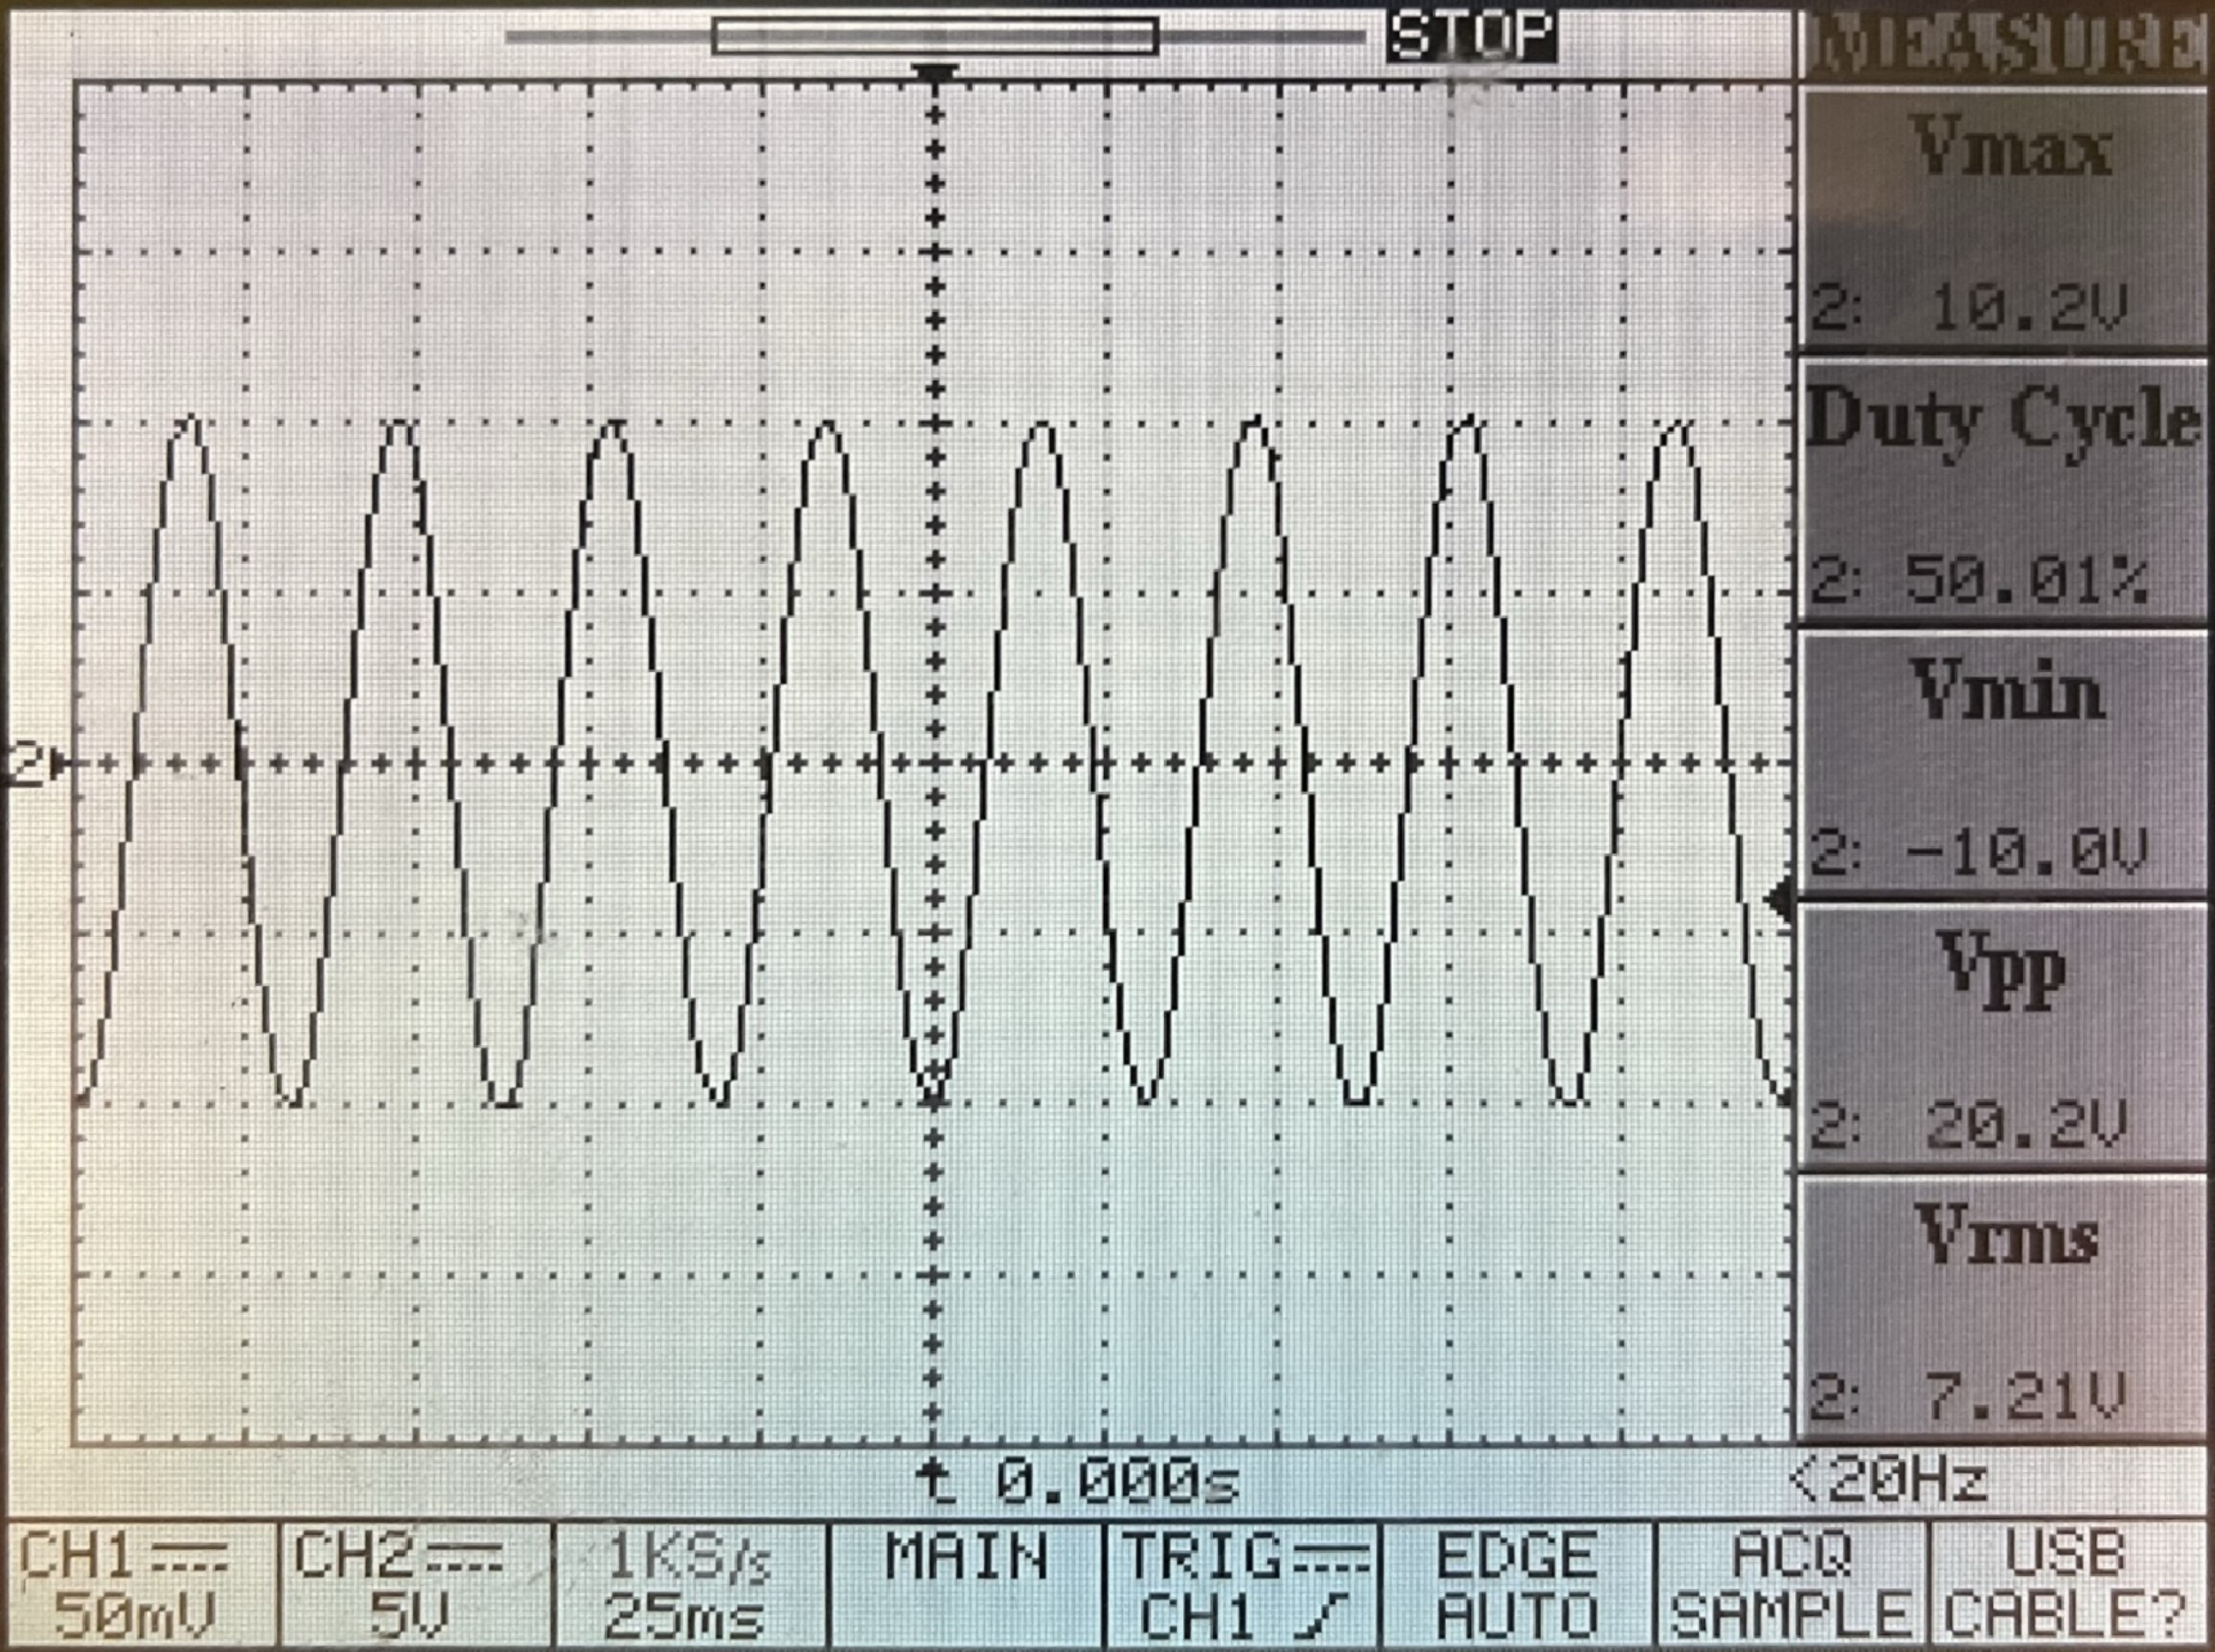
\includegraphics[width=0.6\textwidth]{Figures/flux_test.JPEG}
% 	\caption[Flux Linkage test, oscilloscope output @386rpm.]{Flux Linkage test, oscilloscope output @386rpm.}
% 	\label{fig:flux_measure_oscilloscope} %chktex 24
% \end{figure}

In the example image, the oscilloscope measured a peak voltage of $10.2$, while the rotor was spinning at $386rpm$, which is equivalent to $202rad/s$ electrical velocity. This results in a flux linkage of $0.050 Wb$. The same procedure was repeated at several speeds, and the results are shown in \Cref{fig:flux_linkage_rpm}. In this graph, two other lines are shown, they represent the flux linkage estimated using the torque and speed constant provided in the datasheet. Notice that the experimental data aligns well with the value derived from the voltage constant but it is very different from the value derived from the torque constant. This is probably due to different references and transformations being used, but as there isn't much information available on the datasheet, the measured value is assumed to be the correct one.

% \begin{figure}[!htb]
% 	\centering
% 	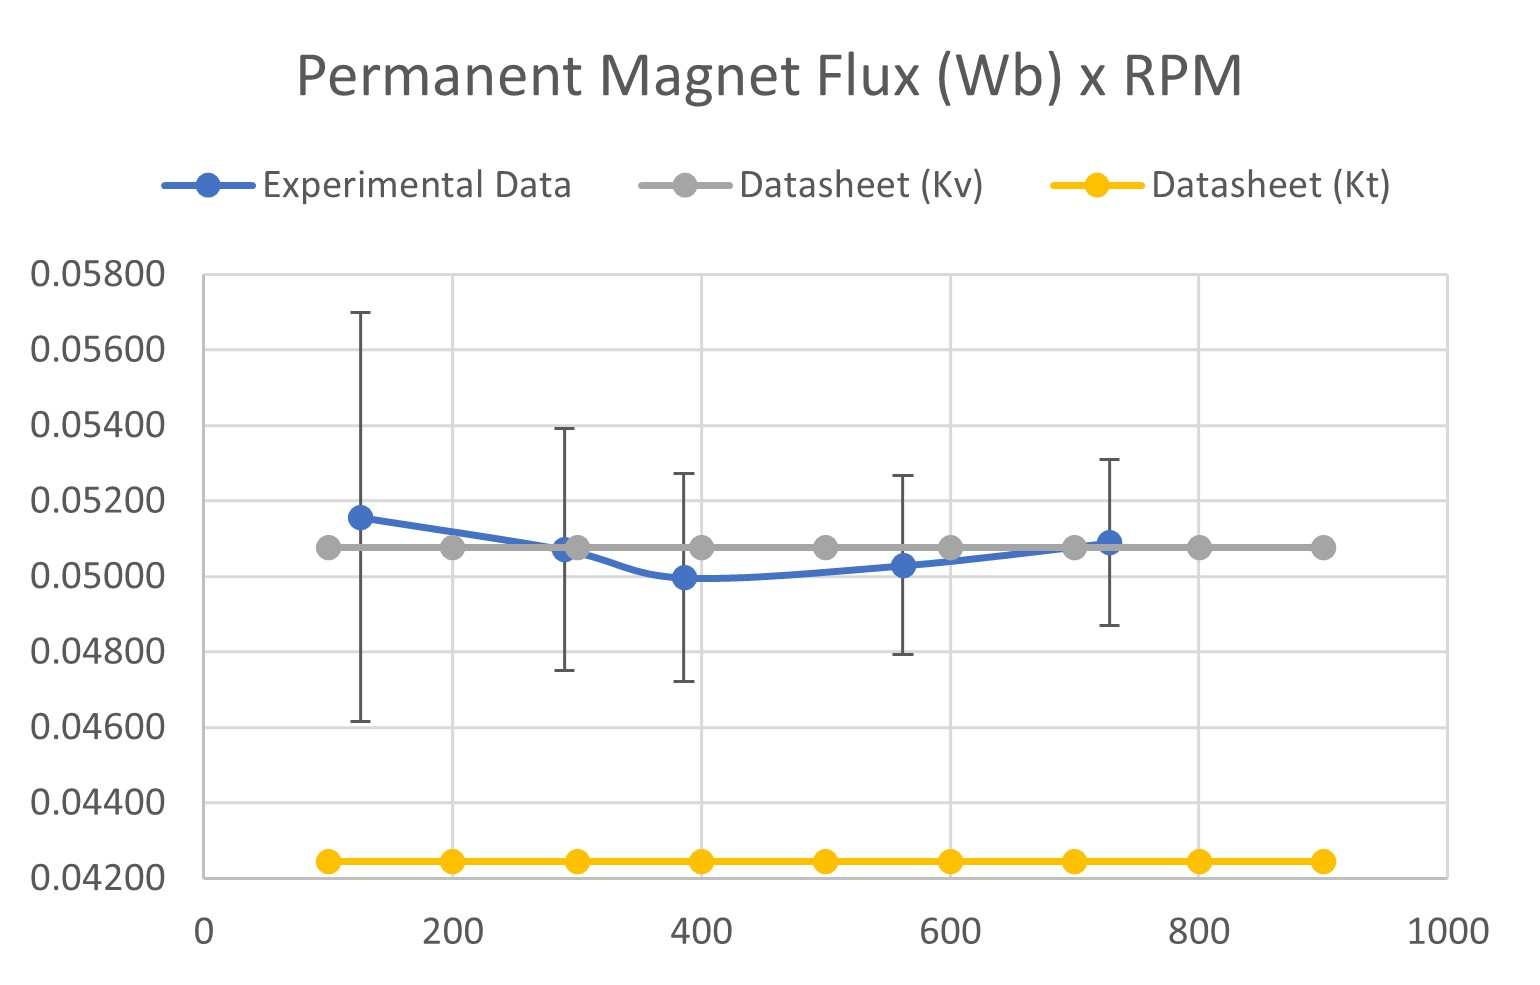
\includegraphics[width=0.5\textwidth]{Figures/flux_linkage_graph.jpg}
% 	\caption[Flux Linkage as a function of RPM.]{Flux Linkage as a function of RPM.}
% 	\label{fig:flux_linkage_rpm} %chktex 24
% \end{figure}
\begin{figure}[!htb]
    \begin{subfigmatrix}{2}
      \subfigure[Oscilloscope output @386rpm]{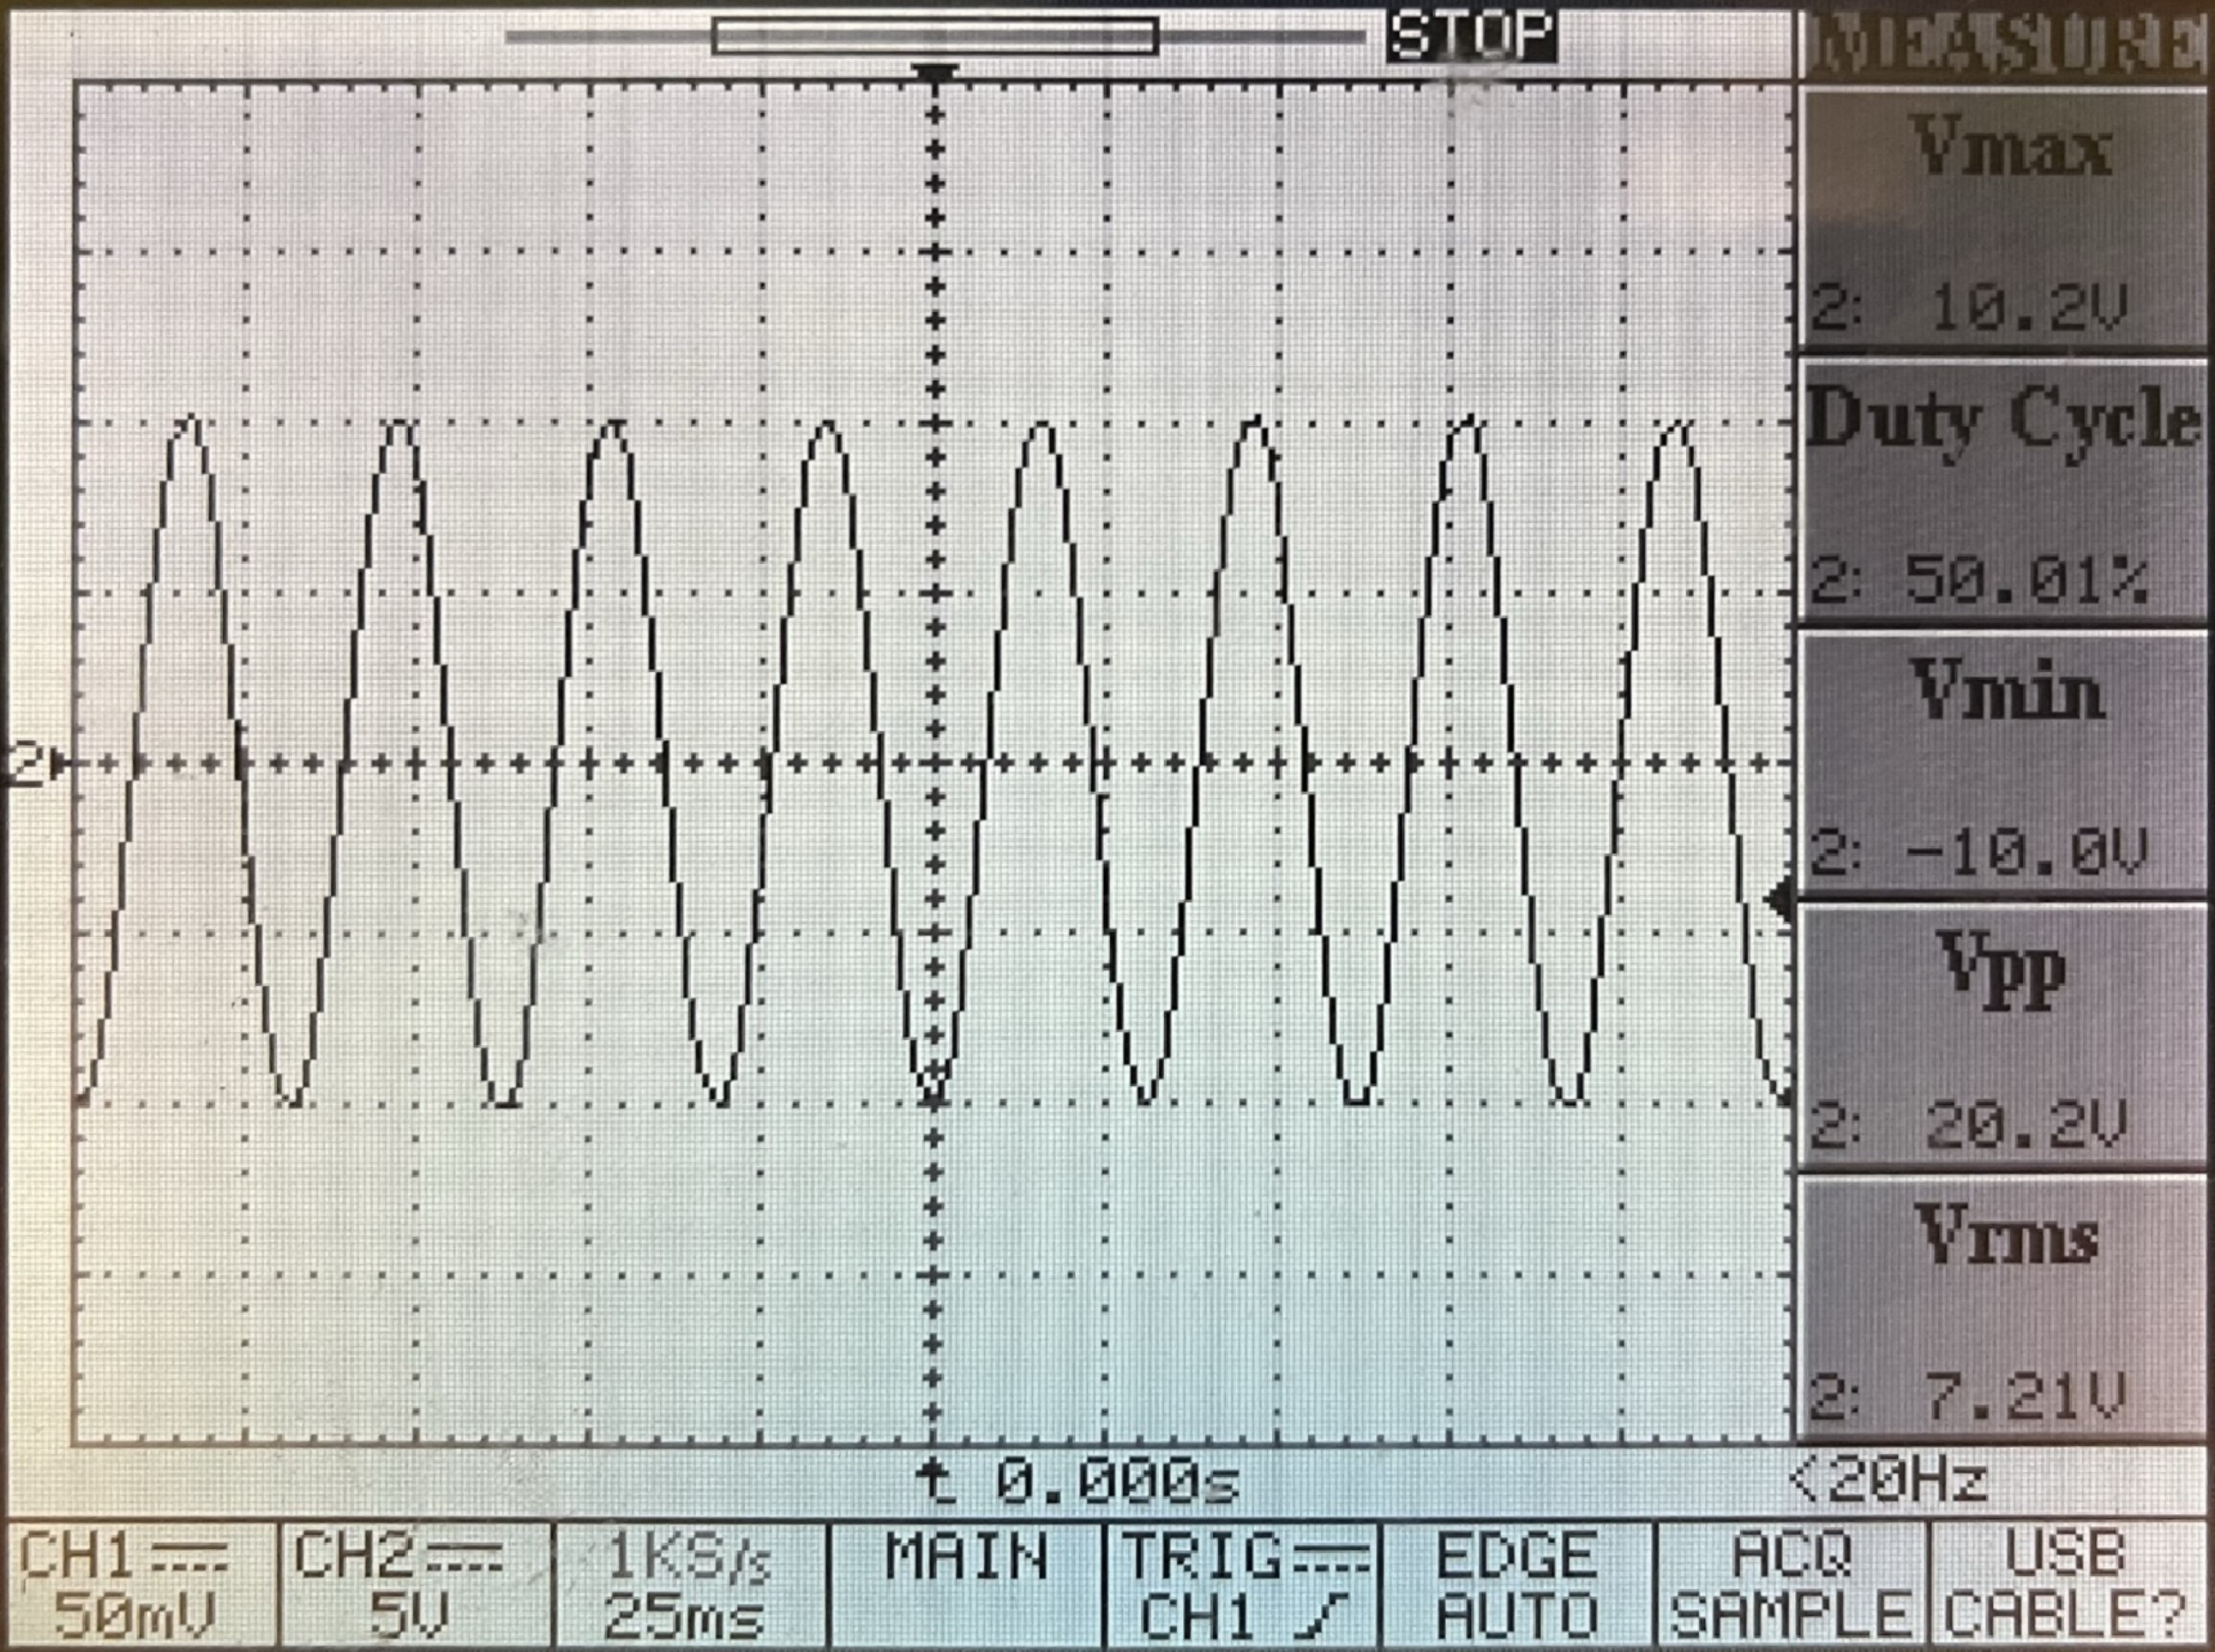
\includegraphics[width=0.51\textwidth]{Figures/flux_test.JPEG}\label{fig:flux_measure_oscilloscope}}
      \subfigure[Flux Linkage as a function of RPM.]{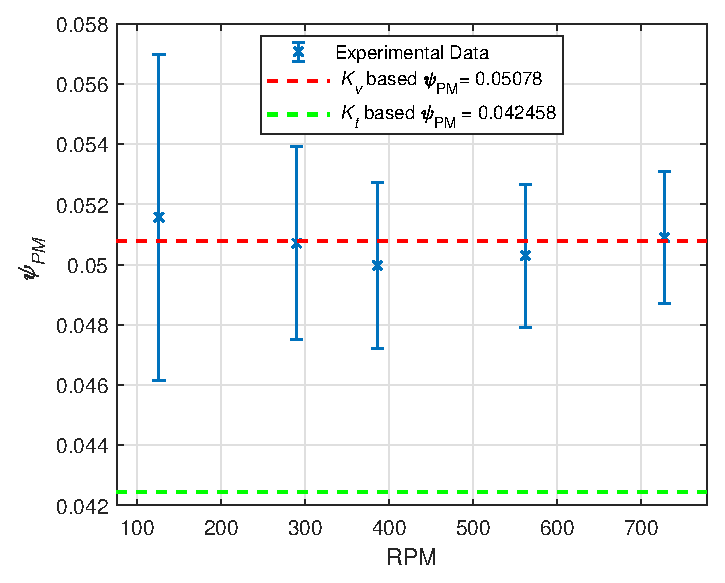
\includegraphics[width=0.45\textwidth]{Figures/Flux_test.eps}\label{fig:flux_linkage_rpm}}
    \end{subfigmatrix}
    \caption{Flux Linkage characterization.}
    \label{fig:flux_linkage_characterization}%chktex 24
\end{figure}

% %%%%%%%%%%%%%%%%%%%%%%%%%%%%%%%%%%%%%%%%%%%%%%%%%%%%%%%%%%%%%%%%%%%%%%%%%%%%%%%%%%%%%%%%%%%%%%%%%%%%%%%%%%%%%%%%%%%%%%%%%%%%%%%%%%%%%%%
% %%%%%%%%%%%%%%%%%%%%%%%%%%%%%%%%%%%%%%%%%%%%%%%%%%%%%%%%%%%%%%%%%%%%%%%%%%%%%%%%%%%%%%%%%%%%%%%%%%%%%%%%%%%%%%%%%%%%%%%%%%%%%%%%%%%%%%%
\subsection{Windings direct and quadrature inductances}
\label{sec:inductance}

To achieve better accuracy, two different methods will be proposed, one using the inverter, and the other only using a DC power supply.
\subsubsection{Method 1}
\label{sec:inductance_method1}

\begin{figure}[!htb]
	\centering
	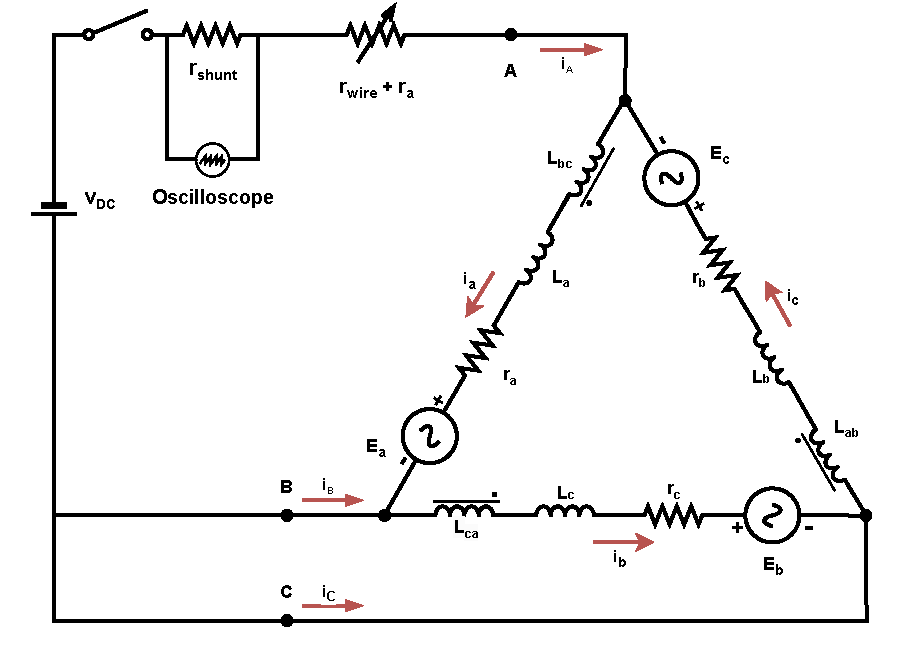
\includegraphics[width=0.6\textwidth]{Figures/Ld_measure.pdf}
	\caption[Inductance measurement setup schematic.]{Inductance measurement setup schematic.}
	\label{fig:Ld_measure_schematic} %chktex 24
\end{figure}

The simpler method, which does not use the inverter, works by measuring the current throughout a voltage step and measuring the time constant of the system. To measure the current, a shunt resistor is used coupled with the same oscilloscope from the previous section (\textit{Promax OD-571}). To achieve a variable current, a variable resistor was used in series with the shunt, as shown in \Cref{fig:Ld_measure_schematic}. The system resistance was measured with the micro ohmmeter from the previous section (\textit{UNI-T UT620A Micro-ohmmeter}), including wire and switch resistance. The experiment setup is shown in \Cref{fig:induc_setup}.
% \begin{figure}[!htb]
%     \begin{subfigmatrix}{2}
%       \subfigure[Schematic]{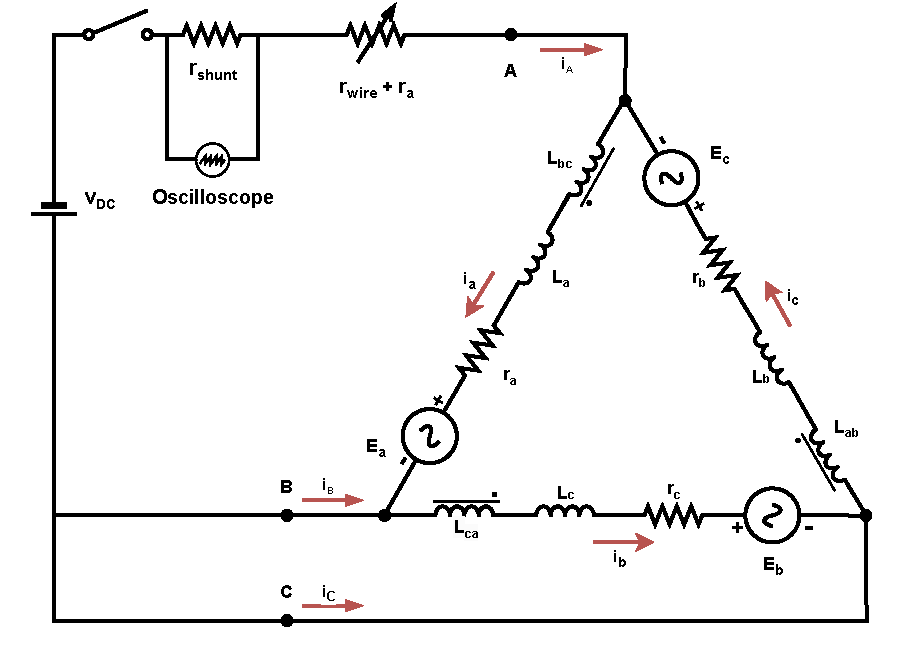
\includegraphics[width=0.49\linewidth]{Figures/Ld_measure.pdf}\label{fig:Ld_measure_schematic}}
%       \subfigure[Actual setup]{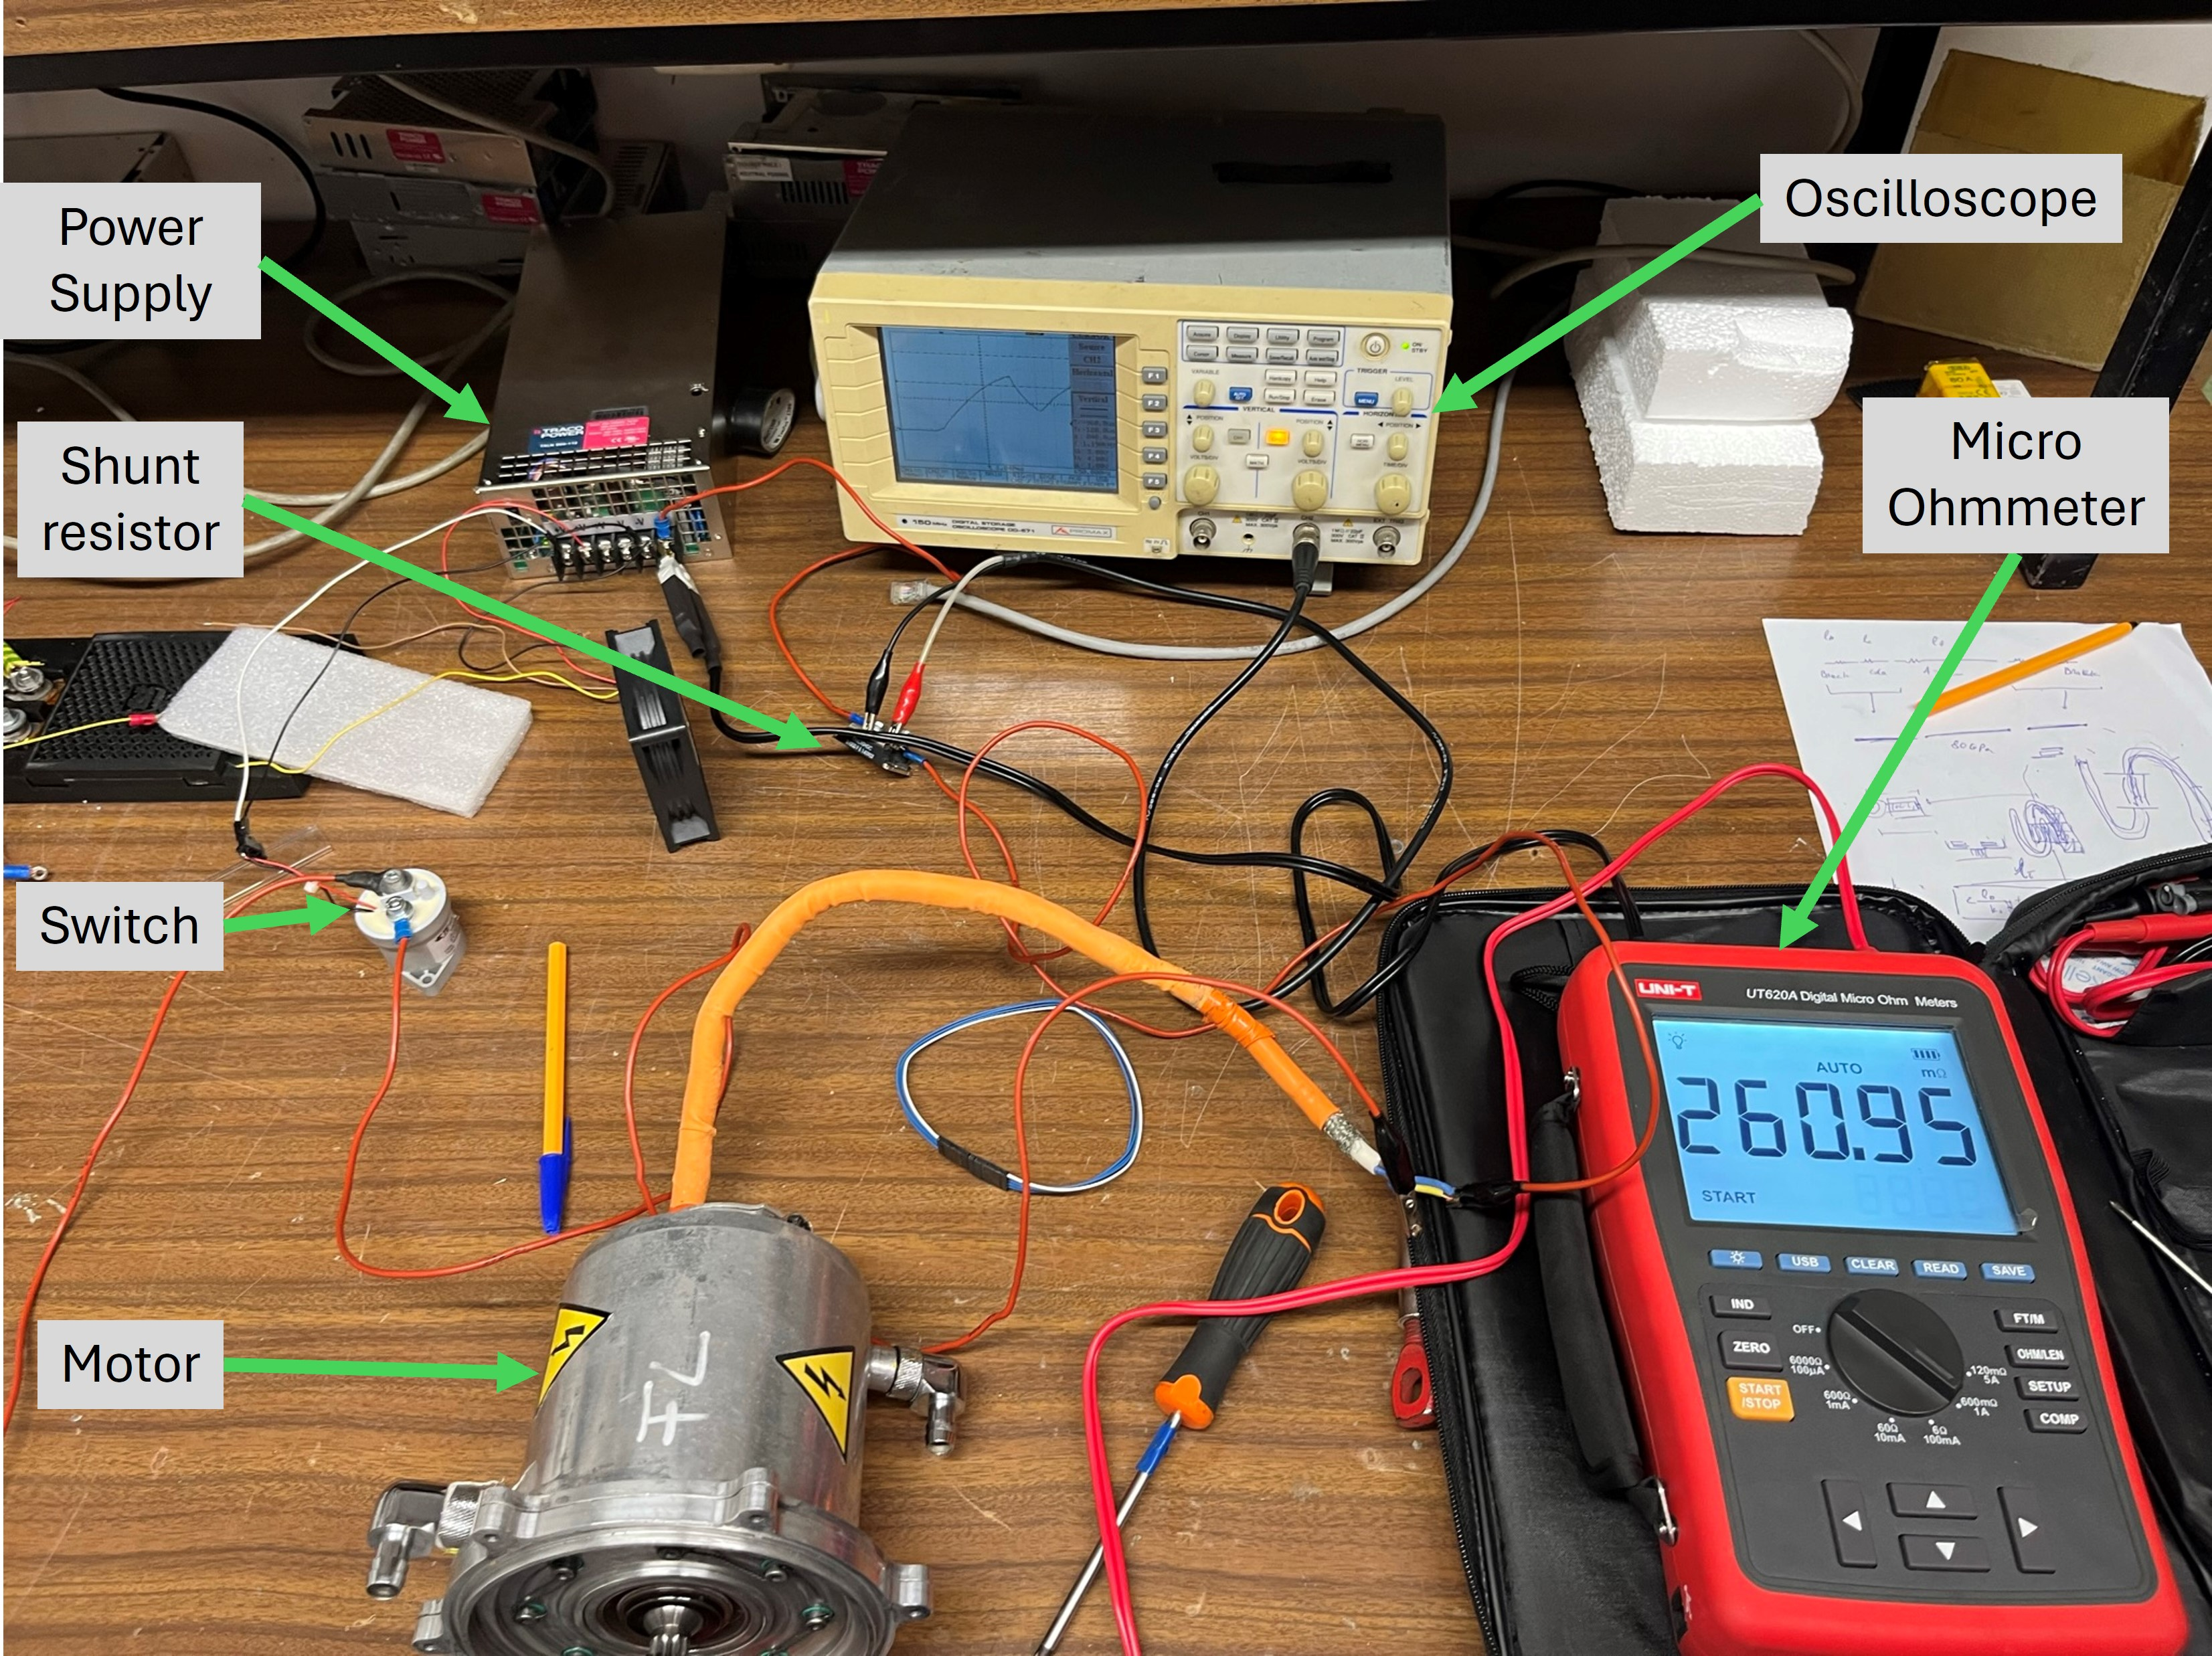
\includegraphics[width=0.49\linewidth]{Figures/induc_test.JPEG}\label{fig:induc_setup}}
%     \end{subfigmatrix}
%     \caption{Inductance measurement setup.}
%     \label{fig:aircrafts}%chktex 24
% \end{figure}


\begin{figure}[!htb]
	\centering
	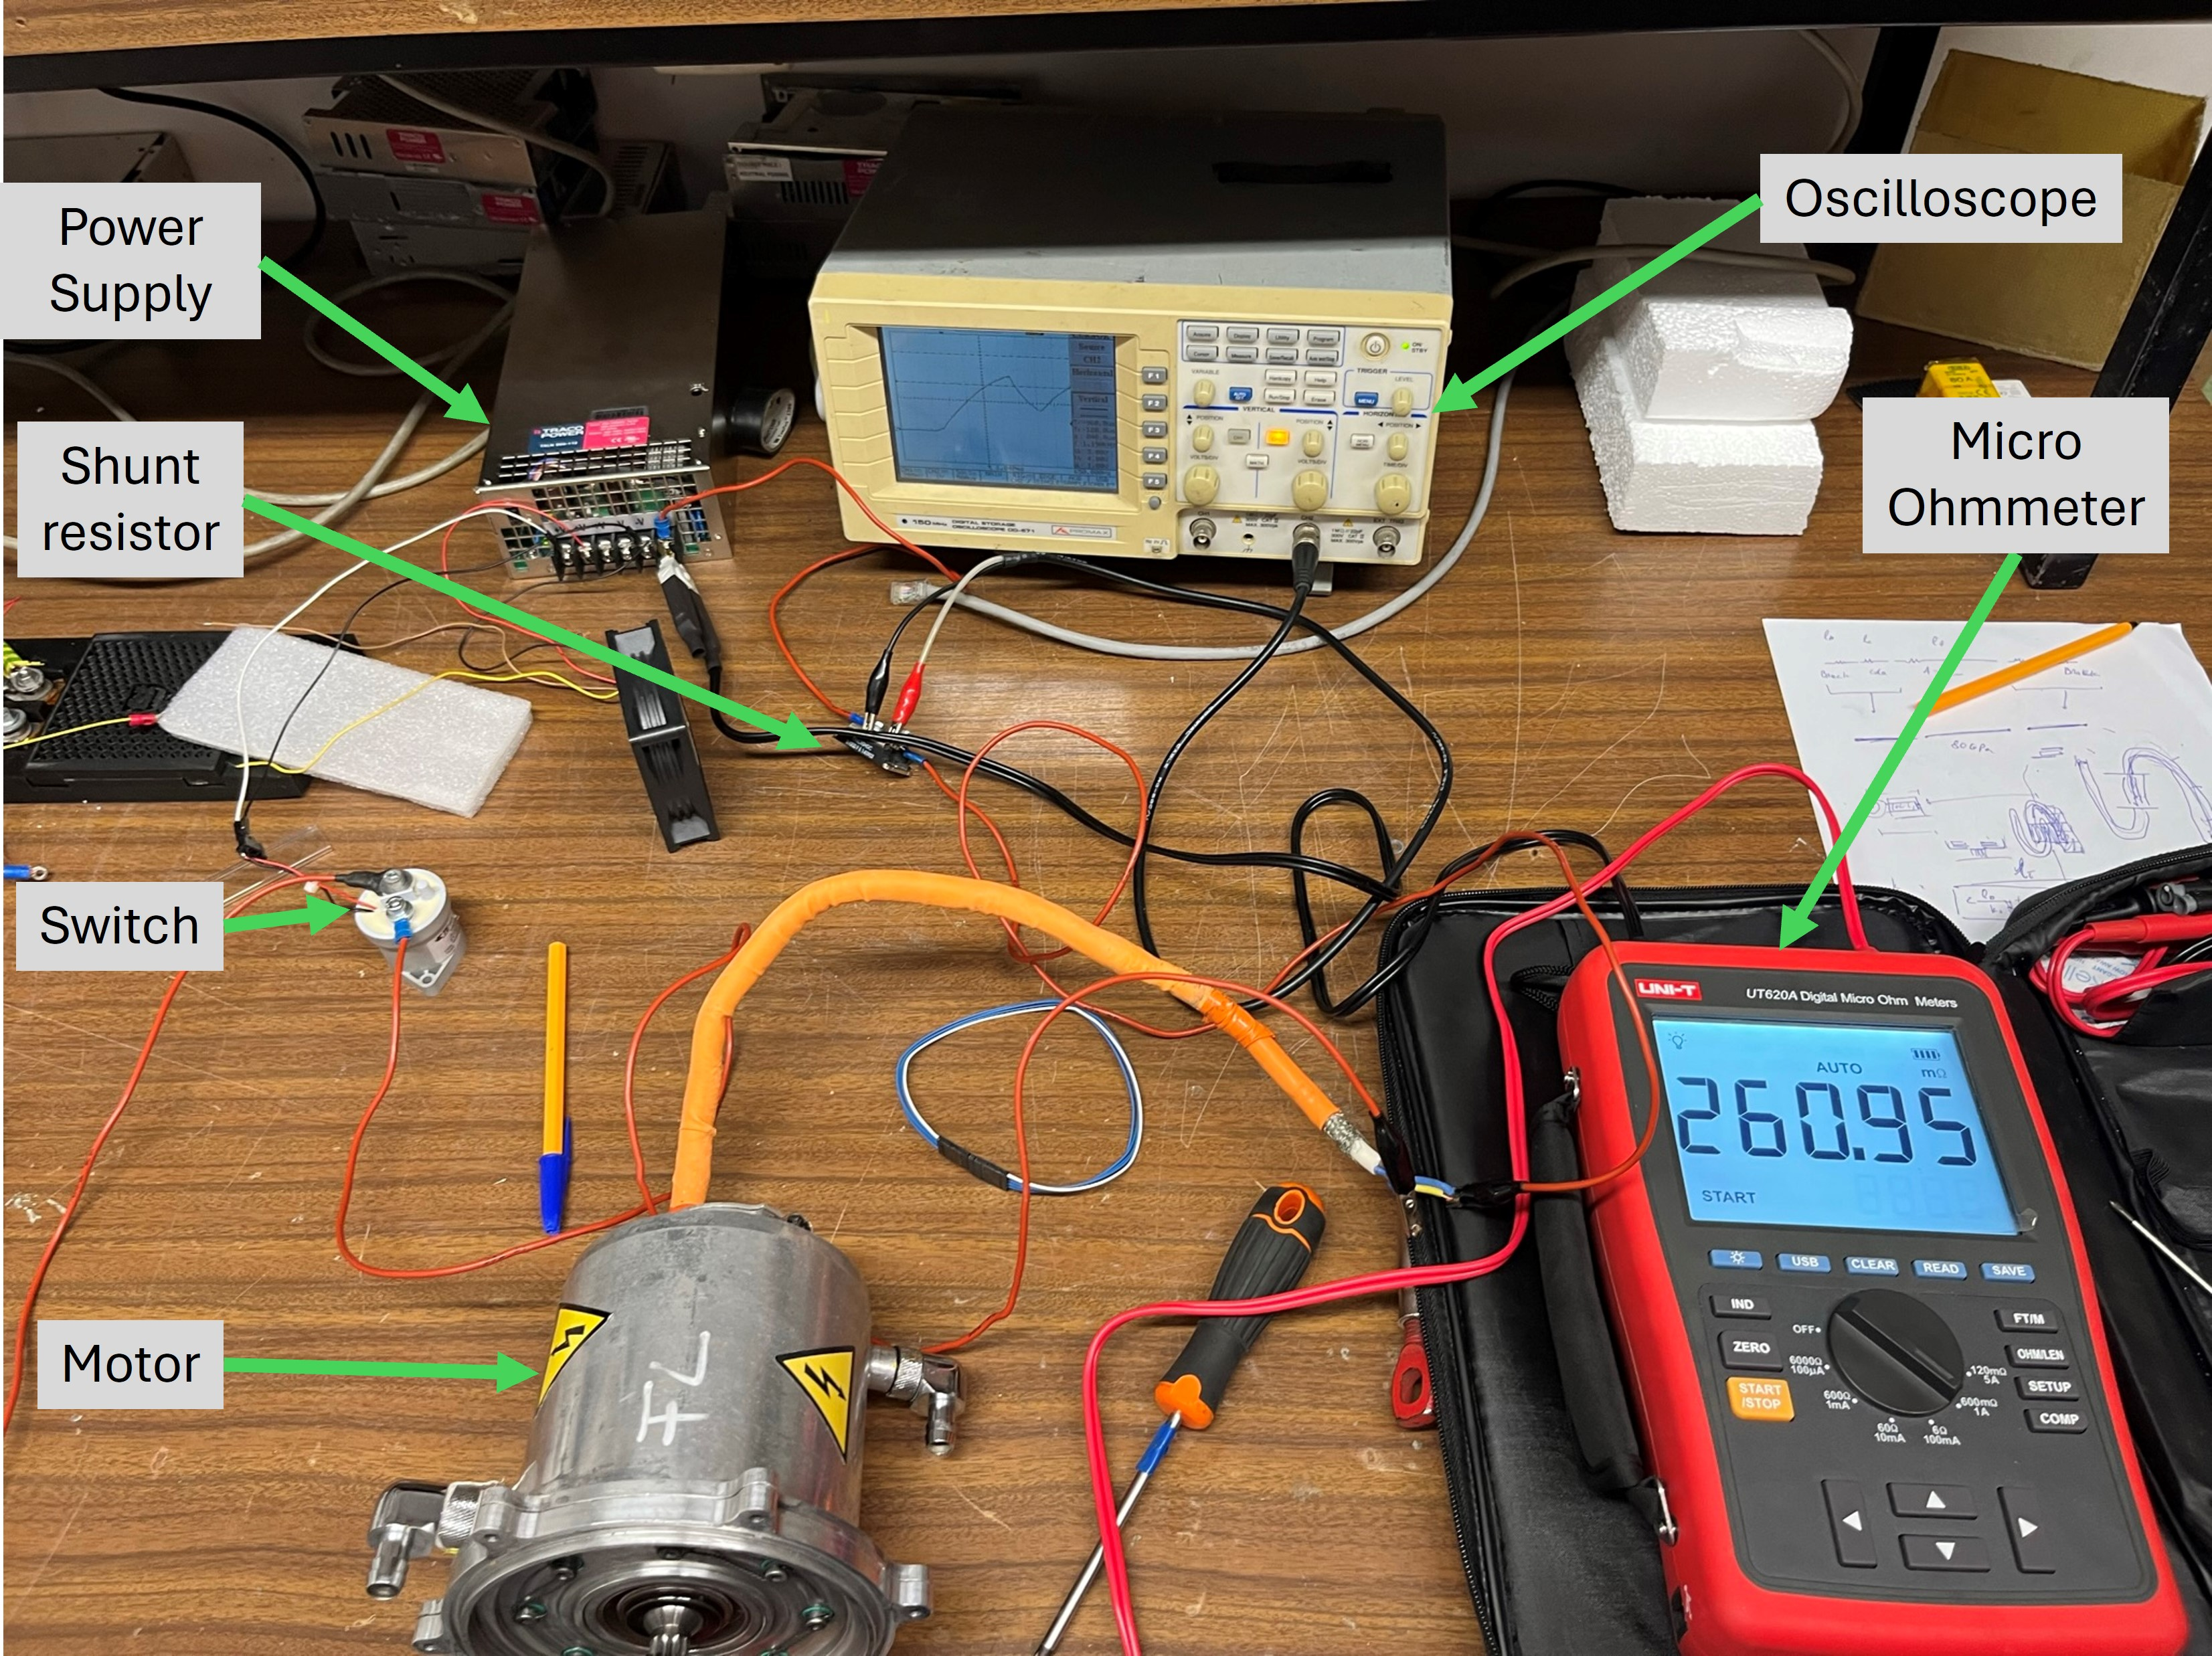
\includegraphics[width=0.6\textwidth]{Figures/induc_test.jpg}
	\caption[Inductance measurement setup.]{Inductance measurement setup.}
	\label{fig:induc_setup} %chktex 24
\end{figure}

\subsubsubsection{Direct Axis}
The direct axis measurement starts with the resistance measurement of the entire setup, motor, wires, switch, and shunt. Then, a quick voltage pulse is applied to align the rotor with the magnetic field, which in this setup is equivalent to the voltage vector $V_6$. In the aligned condition, the current through phase b ($i_b$) is zero, and $i_a = -i_c$. After the rotor is aligned, a new pulse is applied, now for the actual measurement as exemplified in \Cref{fig:inductance_oscilloscope}. The time constant can be retrieved using the basic equation for an RL circuit applied to the shunt resistor (\Cref{eq:rl_circuit,eq:tau}).

\begin{subequations}
	\begin{equation}
		u(t) = i_A r_{shunt}(1-e^{\frac{-t}{\tau}})
		\label{eq:rl_circuit}
	\end{equation}
	\begin{equation}
		\tau = \frac{2L_d}{\frac{r}{2}+r_{wire} + r_a + r_{shunt}}
		\label{eq:tau}
	\end{equation}
\end{subequations}
In \Cref{eq:rl_circuit} $u(t)$ represents the measured voltage on the shunt resistor, $V_{DC}$ is the power supply voltage, $\tau$ is the system time constant, $r_a$ is the variable resistance to adjust the current,$r_{shunt}$ is the shunt resistance, and $r_{wire}$ is the sum of the wire resistances with the switch resistance. 
% To simplify the measurements, instead of calculating the first term $i_A r_{shunt}$, it was replaced by the voltage that which the oscilloscope settled.

\begin{figure}[!htb]
	\centering
	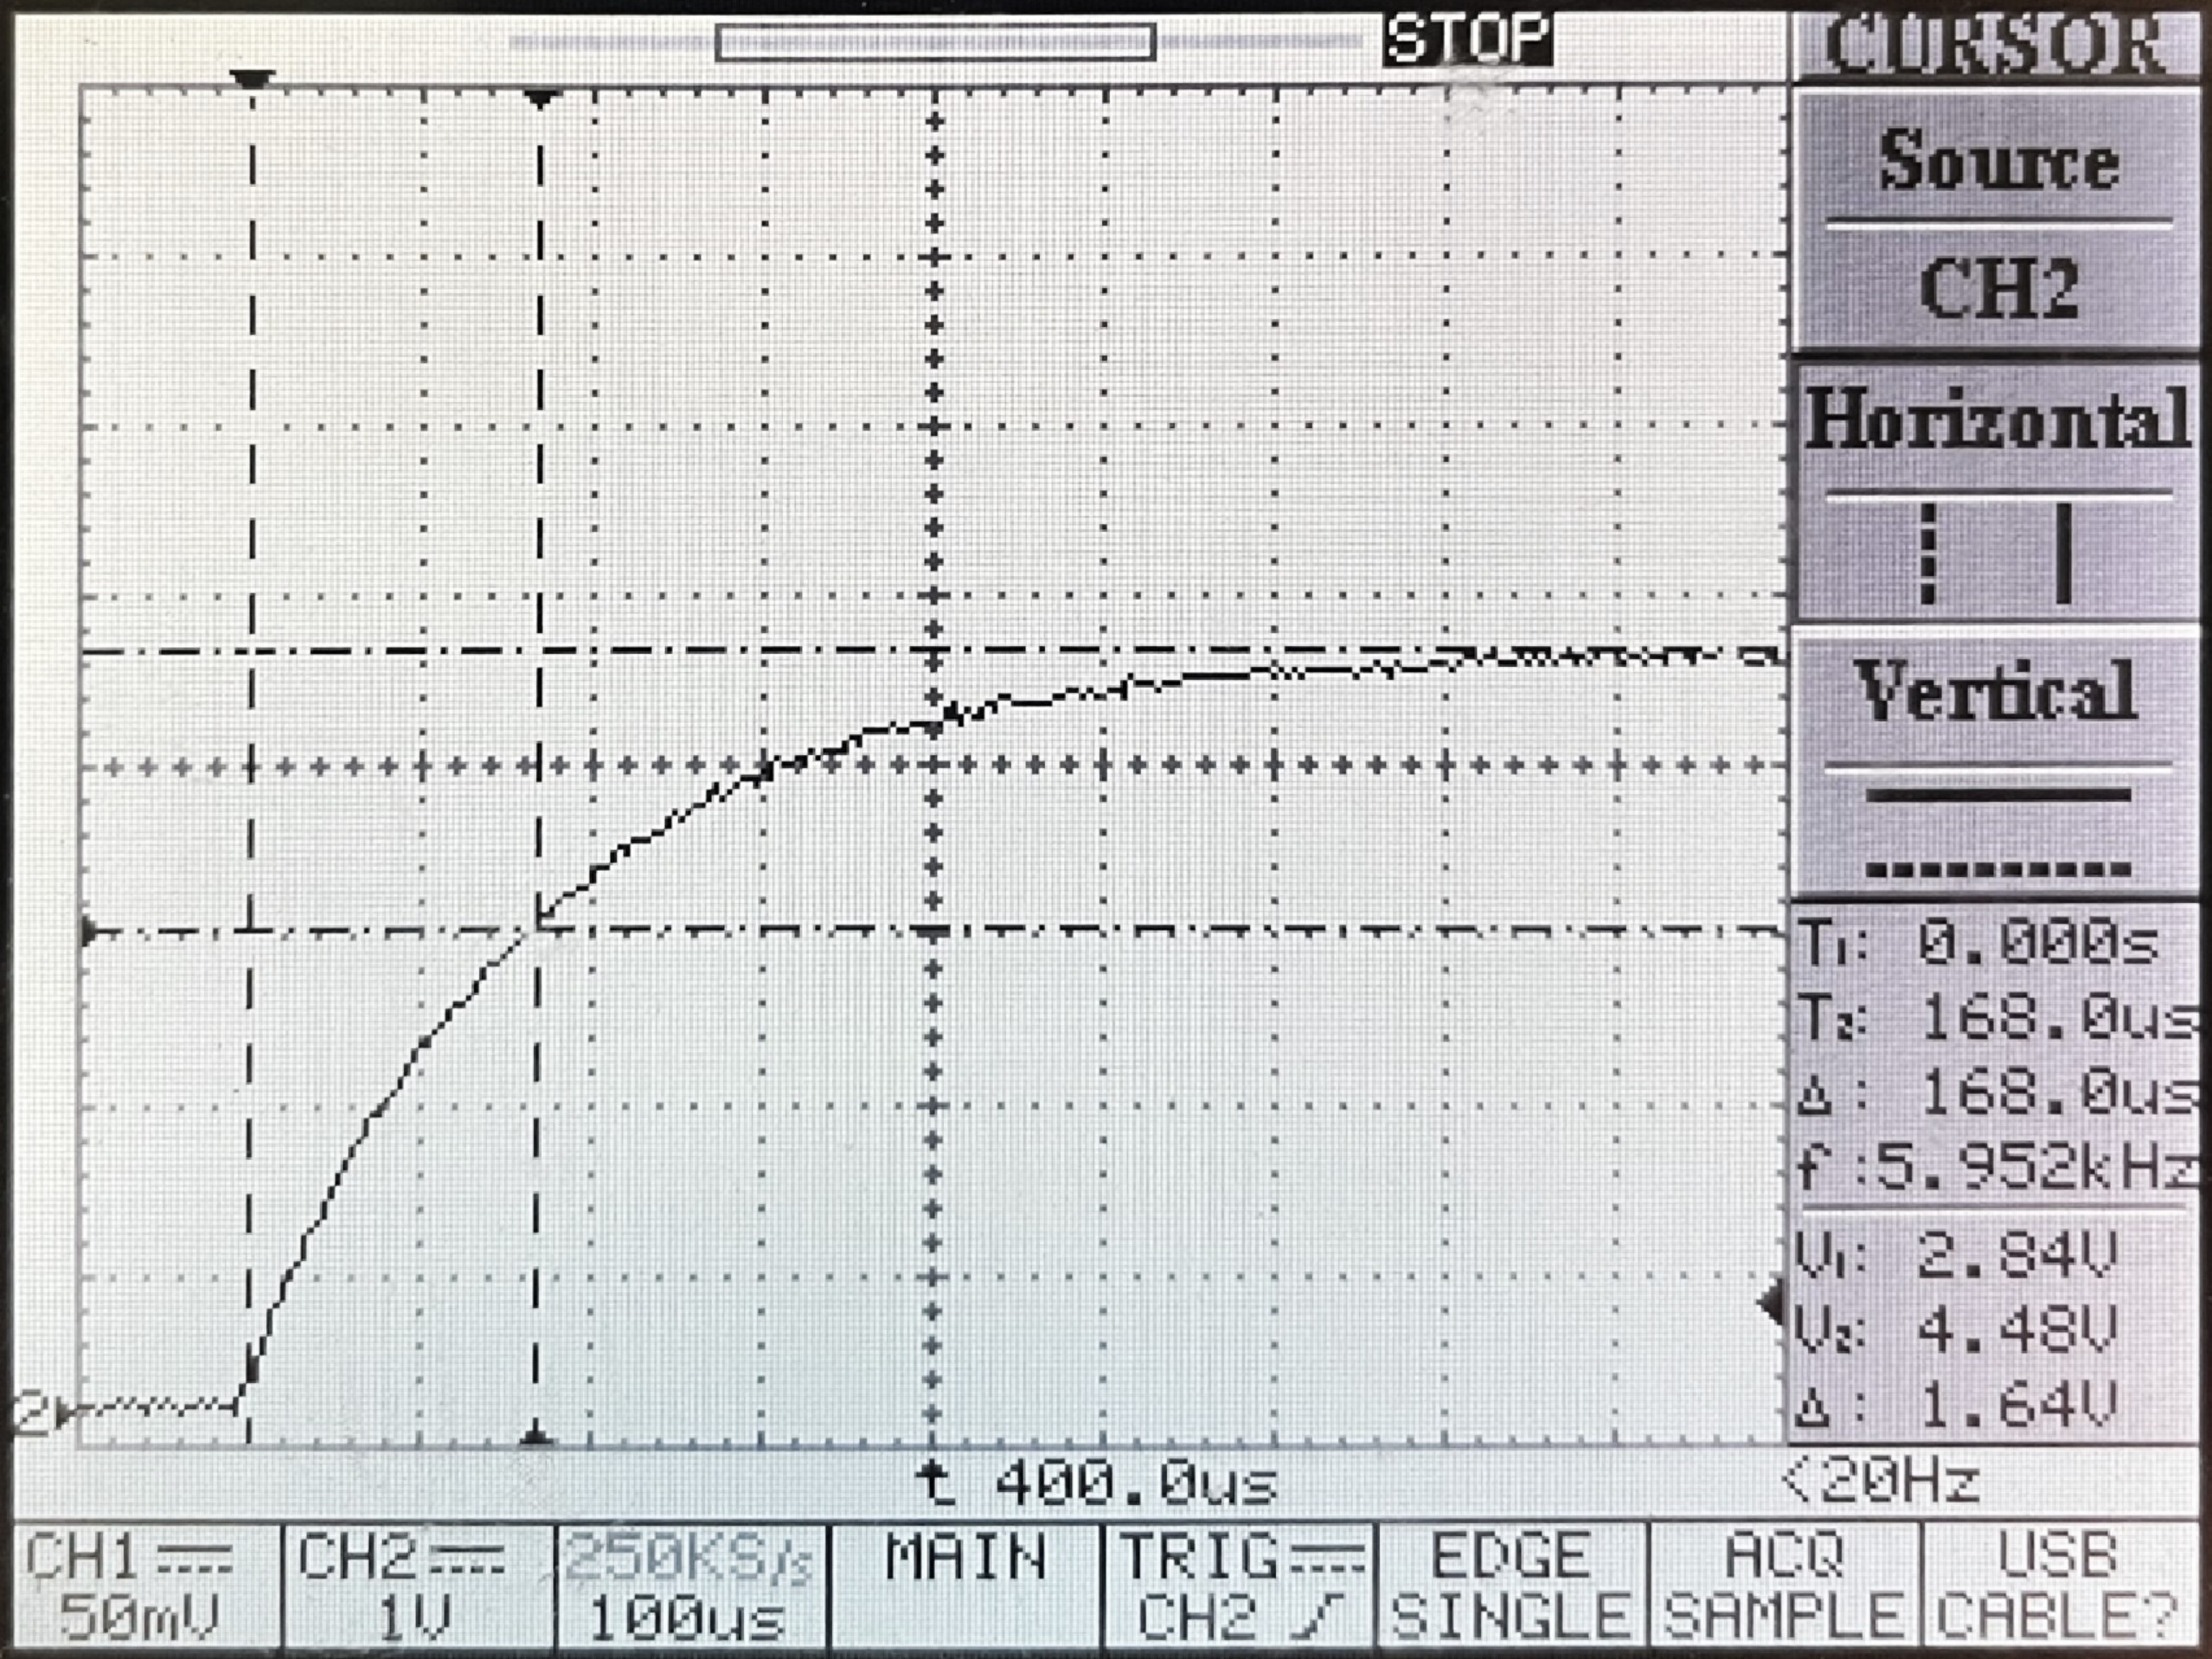
\includegraphics[width=0.5\textwidth]{Figures/induc_oscilloscope.JPEG}
	\caption[Inductance measurement oscilloscope output.]{Inductance measurement oscilloscope output.}
	\label{fig:inductance_oscilloscope} %chktex 24
\end{figure}

With the curve plotted on the oscilloscope, the time constant was measured by evaluating how long it took for the voltage to reach $0.632 i_A r_{shunt}$. Then, with the time constant and the system resistance, the inductance was calculated. Note that this inductance was measured for a phase current of half the line current, resulting in a direct axis current of $i_d = \frac{i_A}{\sqrt{3}}$.

The inductance variation with current is not symmetrical in the current axis, as the permanent magnet offsets the magnetic curve, causing saturation with very small positive currents in the direct axis. Although simple, this method has the drawback of not measuring the variation of inductance in the field weakening operating range, only on the field intensifying range that is not often used. To measure in the field weakening range it is necessary to lock the rotor after the initial pulse, and then invert the power supply polarity.

\begin{figure}[!htb]
	\centering
	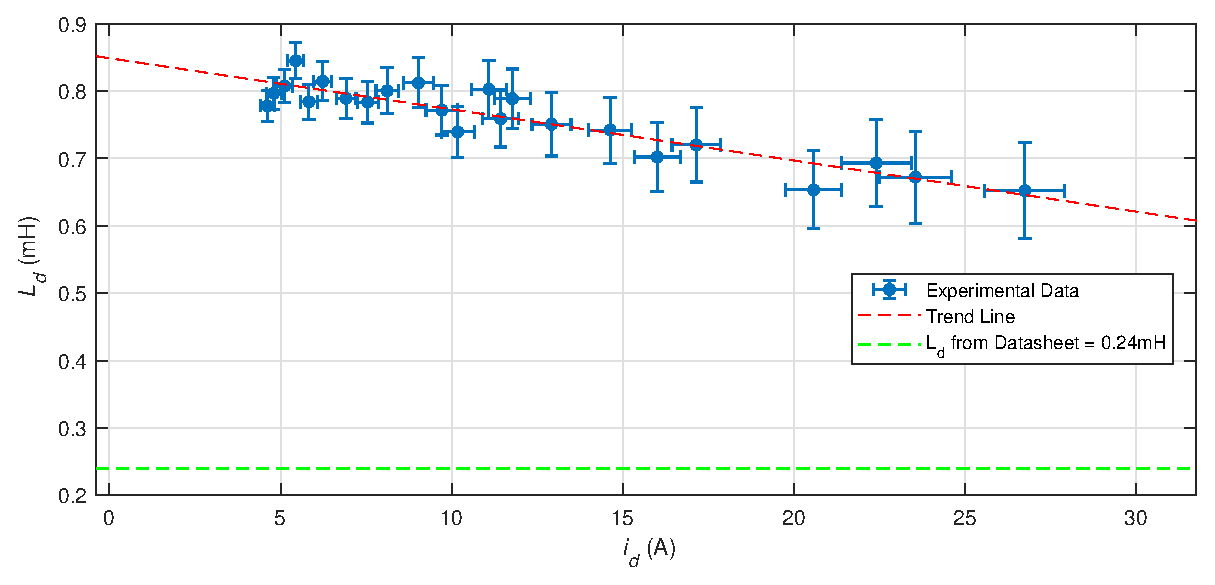
\includegraphics[width=1\textwidth]{Figures/Ld_id.eps}
	\caption[$L_d$ in function of $i_d$.]{$L_d$ in function of $i_d$.}
	\label{fig:ld_graph} %chktex 24
\end{figure}

The test results are shown in \Cref{fig:ld_graph}, and as with the flux linkage, there is a great difference between the measured data and the value from the datasheet. The saturation effects are clear and start with very little current, as predicted.




\subsubsubsection{Quadrature Axis}
The quadrature axis measurement is very similar to the direct axis, with only two differences. The first change is on the alignment pulse, instead of shorting the B and C terminals and applying the pulse from A to BC as done for the direct inductance measurement, the pulse is only applied from B to C as shown in \Cref{fig:quad_induc_setup_prep}. This will align the rotor with the phase b axis allowing it to be locked in a position electrically orthogonal to the resultant voltage of a pulse from A to BC\@. That is the second difference, after the alignment an external tool is necessary to lock the rotor in place. The rest of the procedure is the same as the direct axis measurement.

\begin{figure}[!htb]
	\centering
	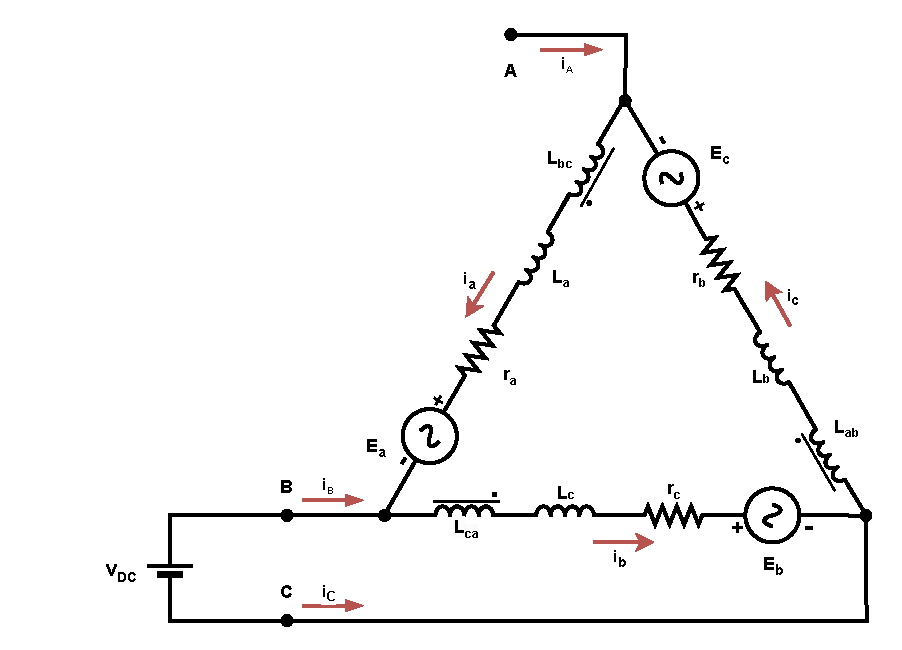
\includegraphics[width=0.7\textwidth]{Figures/Lq_measure_prep.pdf}
	\caption[Quadrature Inductance measurement alignment pulse setup.]{Quadrature Inductance measurement alignment pulse setup.}
	\label{fig:quad_induc_setup_prep} %chktex 24
\end{figure}

The results of the quadrature inductance are shown in \Cref{fig:lq_graph}. It is important to note that as there isn't a reminiscent magnetic flux in the quadrature axis, the variation of the inductance with current is symmetrical in the current axis, and only shows signs of saturation at high currents.

\begin{figure}[!htb]
	\centering
	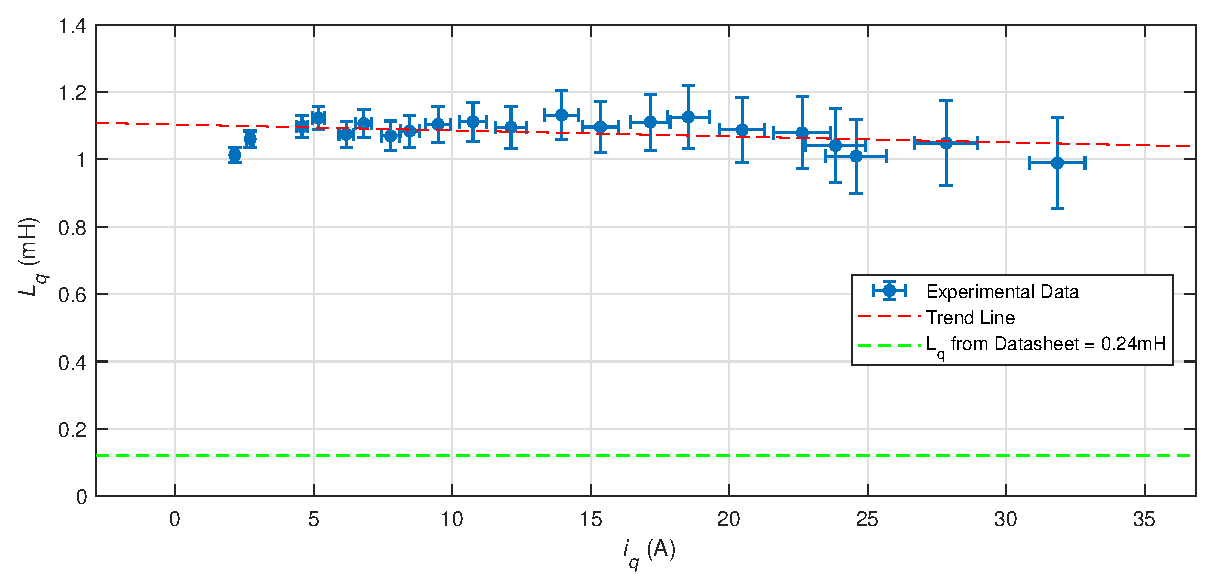
\includegraphics[width=1\textwidth]{Figures/Lq_iq.eps}
	\caption[$L_q$ in function of $i_q$.]{$L_q$ in function of $i_q$.}
	\label{fig:lq_graph} %chktex 24
\end{figure}

\subsubsection{Method 2}

The second method for inductance characterization is according to~\citet{Stumberger:saturation_model:2003}. It uses a \gls{vsi} coupled with a control algorithm to keep the current in one of the axis constant, and then do a voltage step in the other axis. This measurement also needs to be done in a locked rotor position, but it has the advantage of characterizing the cross-magnetization effect. The rotor needs to be locked to allow the simplification shown in \Cref{eq:motor_with_no_omega}, resulting in \Cref{eq:inductance_voltage_step}.

\begin{subequations}
	\begin{equation}
		u_d = ri_d(t) + \frac{d\psi_d (t)}{dt} - \psi_q \cancelto{0}{\omega_e}
	\end{equation}
	\begin{equation}
		u_q = ri_q(t) + \frac{d\psi_q (t)}{dt} + \left(\psi_d + \psi_{PM}\right) \cancelto{0}{\omega_e}
	\end{equation}
	\label{eq:motor_with_no_omega}
\end{subequations}


\begin{subequations}
	\begin{equation}
		\frac{d\psi_d (t)}{dt} = u_d - ri_d(t)
	\end{equation}
	\begin{equation}
		\frac{d\psi_q (t)}{dt} = u_q - ri_q(t)
	\end{equation}
	\label{eq:inductance_voltage_step}
\end{subequations}

This method defines the flux linkage based on the integration of \Cref{eq:inductance_voltage_step}, and to measure the flux linkage variation in the quadrature axis, it performs a series of stepwise voltage changes in $u_q$ while maintaining the current $i_d$ constant (\Cref{fig:stepwise}). The integration of those curves will result in the quadrature flux linkage variation with $i_q$. These steps are repeated for several values of $i_d$, and for each of them, a flux linkage curve is created as shown in \Cref{fig:flux_linkage_curve}. Note that this figure was generated as a concatenation of two separate voltage steps, one positive and one negative, to simplify the process. This concatenation is the reason for the small misalignment in the flux linkage lines near the origin.

Instead of using the measured value for the phase resistance, its value is estimated by assuming the current is at a steady state at the end of the voltage pulse so that the flux linkage is stable and $u_x = ri_x$, this is done to reduce integration errors on the flux linkage and also to account for wires, connections, and \gls{mosfet} resistances.

\begin{figure}[!htb]
	\begin{subfigmatrix}{2}
		\subfigure[Voltage]{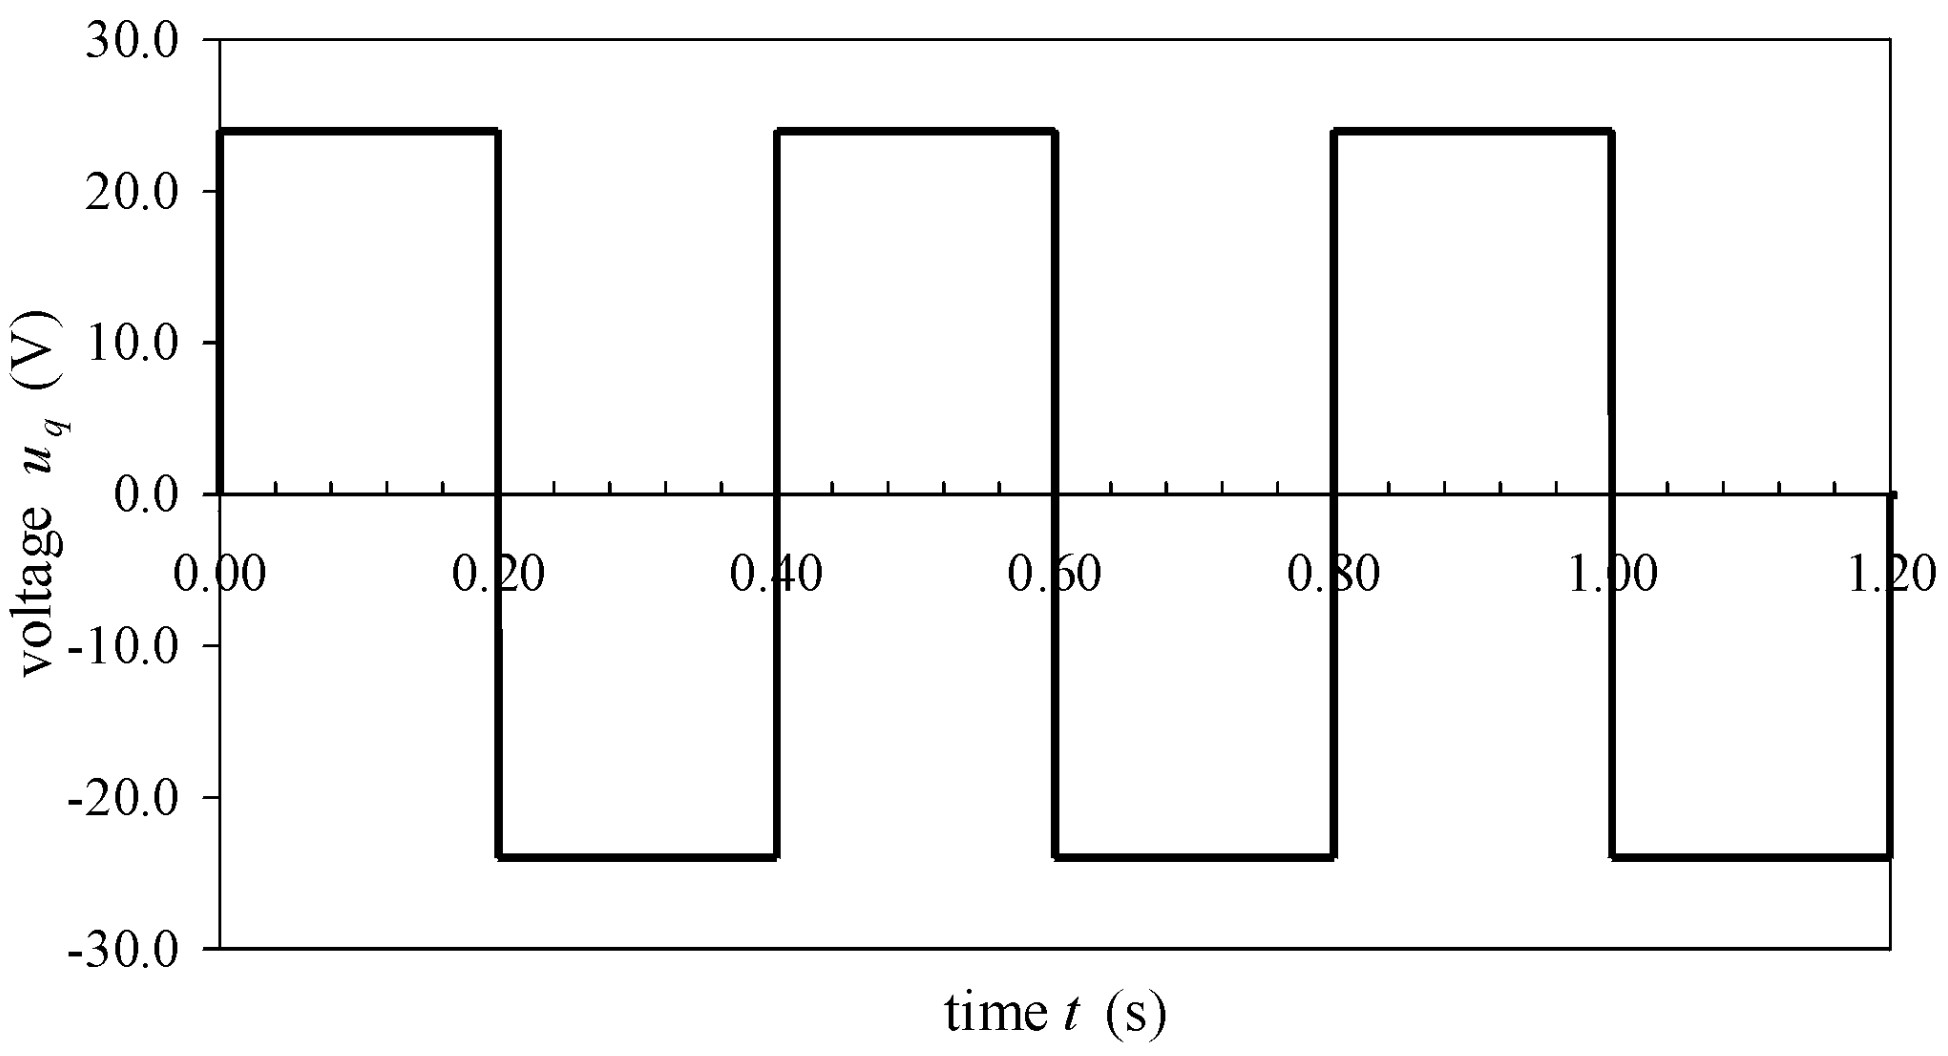
\includegraphics[width=0.49\linewidth]{Figures/stepwise_uq.jpg}\label{fig:stepwise_uq}}
		\subfigure[Currents]{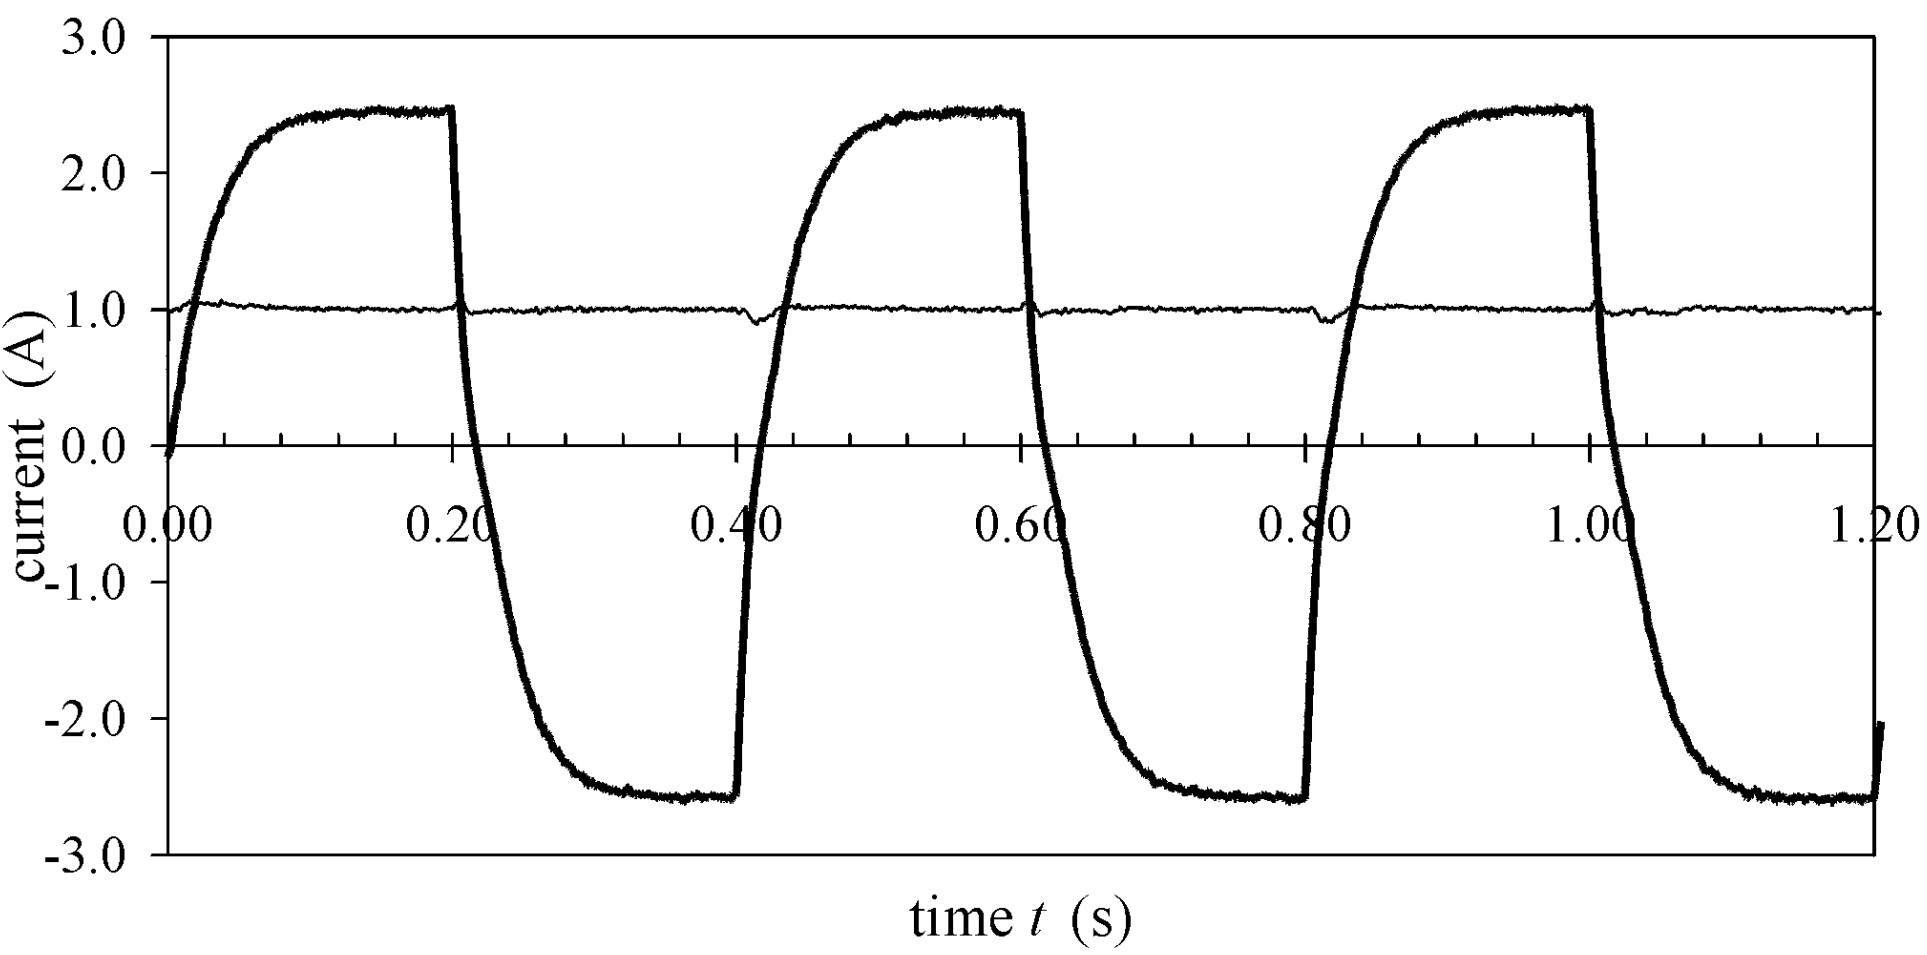
\includegraphics[width=0.49\linewidth]{Figures/stewise_currents_response.jpg}\label{fig:stepwise_currents}}
	\end{subfigmatrix}
	\caption{Identification voltage pulses - from~\citet{Stumberger:saturation_model:2003}.}
	\label{fig:stepwise}%chktex 24
\end{figure}
\begin{figure}[!htb]
	\centering
	\includegraphics[width=0.6\textwidth]{Figures/id-5__vq-30.eps}
	\caption[Quadrature Flux linkage @$i_d = -5$A.]{Quadrature Flux linkage @$i_d = -5$A.}
	\label{fig:flux_linkage_curve} %chktex 24
\end{figure}

The same procedure is used for measuring $\psi_d$, but this time the quadrature current is fixed and the direct voltage is changed in stepwise form. Although the original method is proposed to characterize cross-magnetization effects, the results shown in \Cref{fig:all_pulses} present little variation with currents on the perpendicular axis, thus to simplify the study they are approximated as independent. This approximation is used to reduce the dimensionality of the current reference table and to reduce the used space on the \gls{fpga}. To improve the efficiency of the process the quadrature flux linkage was not characterized for positive and negative currents, as the direct axis was, but only for negative currents. Due to the symmetry of the motor, the quadrature axis results were mirrored to create the flux values for positive and negative currents, as shown in \Cref{fig:all_pulses}.

\begin{figure}[!htb]
	\centering
	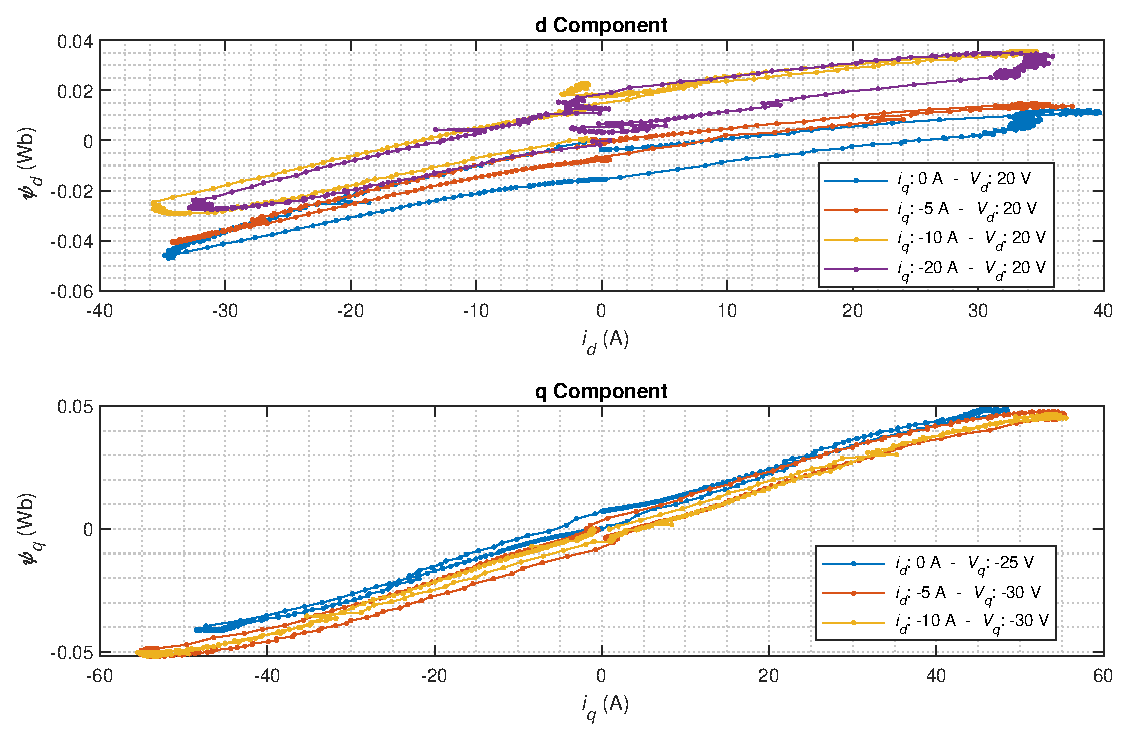
\includegraphics[width=1\textwidth]{Figures/all_pulses.eps}
	\caption[Flux linkage with different currents on a perpendicular axis.]{Flux linkage with different currents on a perpendicular axis.}
	\label{fig:all_pulses} %chktex 24
\end{figure}
%explain about the fit  and the derivative, reinforece that we decided to not account for crossmagnetization to simplify the computations and reduce the size of the lookup table
After the characterization of the fluxes, an exponential fit is done to the data as shown in \Cref{fig:inductances_method_2}. This fit is made disregarding cross magnetization effects, as explained before, and uses the format of \Cref{eq:flux_linkage_fit}. This allows analytical differentiation, resulting in \Cref{eq:flux_derivative_inductance}. This derivative is the inductance value for the given current on the respective axis.
%	\psi_x = ( a1*exp(-b1*x)+ a2*exp(-b2*x)) + c + c_up*((1)/(a4*exp(-b4*x)+1))+c_down*(1-((1)/(a3*exp(-b3*x)+1)))
\begin{equation}
	\psi_x = ( a_1 \cdot e^{-b_1 \cdot x}+ a_2 \cdot e^{-b_2 \cdot x}) + c_{down}\left(1-\left(\frac{1}{a_3 \cdot e^{-b_3 \cdot x}+1}\right)\right) + c_{up} \left(\frac{1}{a_4 \cdot e^{-b_4 \cdot x}+1}\right) + c
	\label{eq:flux_linkage_fit}
\end{equation}
% Here a repeated subscript represents the self-inductance, while multiple subscript identifiers represent mutual inductances due to crossmagnetization.

\begin{figure}[!htb]
	\centering
	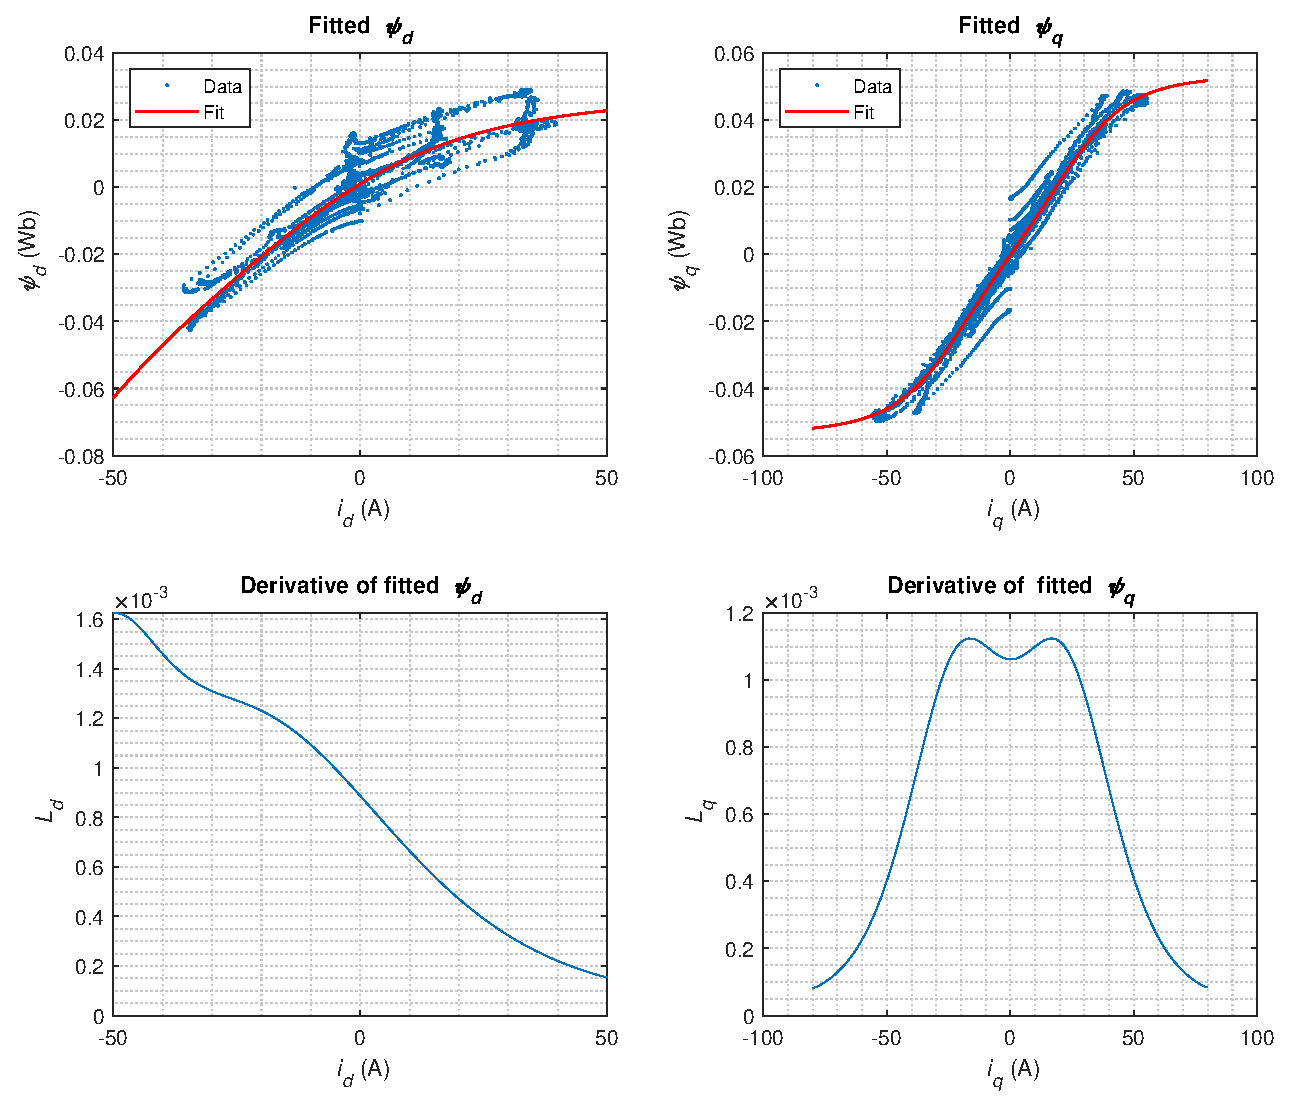
\includegraphics[width=1\textwidth]{Figures/Ldq.eps}
	\caption[Flux Linkage exponential fit.]{Flux Linkage exponential fit. The blue dots are the measured flux linkage, while the red line is the exponential fit (R-square 0.8879 for $\psi_d$ and 0.9681 for $\psi_q$). The bottom plots show the inductances as the derivative of the fit.}
	\label{fig:inductances_method_2} %chktex 24
\end{figure}
\begin{subequations}
		\noindent
		\begin{minipage}{.5\linewidth}
			\begin{equation}
				L_{d} = \frac{\partial \psi_d}{\partial i_d} \approx \frac{\Delta \psi_d}{\Delta i_d}
				% \at[\bigg]{i_q=\text{const.}}
			\end{equation}
		\end{minipage}%
		\begin{minipage}{.5\linewidth}
			\begin{equation}
				L_{q} = \frac{\partial \psi_q}{\partial i_q} \approx \frac{\Delta \psi_q}{\Delta i_q}
				% \at[\bigg]{i_d=\text{const.}}
			\end{equation}
		\end{minipage}%\\
		\label{eq:flux_derivative_inductance}
	\end{subequations}
% \begin{subequations}
% 	\noindent
% 	\begin{minipage}{.5\linewidth}
% 		\begin{equation}
% 			L_{dd} = \frac{\partial \psi_d}{\partial i_d} \approx \frac{\Delta \psi_d}{\Delta i_d}\at[\bigg]{i_q=\text{const.}}
% 		\end{equation}
% 	\end{minipage}%
% 	\begin{minipage}{.5\linewidth}
% 		\begin{equation}
% 			L_{qq} = \frac{\partial \psi_q}{\partial i_q} \approx \frac{\Delta \psi_q}{\Delta i_q}\at[\bigg]{i_d=\text{const.}}
% 		\end{equation}
% 	\end{minipage}%\\
% 	\\
% 	\begin{minipage}{.5\linewidth}
% 		\begin{equation}
% 			L_{dq} = \frac{\partial \psi_d}{\partial i_q} \approx \frac{\Delta \psi_d}{\Delta i_q}\at[\bigg]{i_d=\text{const.}}
% 		\end{equation}
% 	\end{minipage}%
% 	\begin{minipage}{.5\linewidth}
% 		\begin{equation}
% 			L_{qd} = \frac{\partial \psi_q}{\partial i_d} \approx \frac{\Delta \psi_q}{\Delta i_d}\at[\bigg]{i_q=\text{const.}}
% 		\end{equation}
% 	\end{minipage}%
% 	\label{eq:flux_derivative_inductance}
% \end{subequations}

The resultant inductances are shown in \Cref{fig:inductances_method_2}. The fit has a R-squared value of $0.8879$ for the direct axis and $0.9681$ for the quadrature axis. The increased error in the direct axis is due to the cross magnetization effects that were not accounted for in the fit.

Ideally, this test should be performed with a voltage pulse big enough to cover the full current range of the machine, but the available hardware was not capable of reaching such currents, thus the limited range. Despite the limitations, the inductance values using this method closely match with the ones found using method 1 from \Cref{sec:inductance_method1}. This not only increases the confidence in the results but also enables the formulation of a calibration routine on the inverter software that, given some adaptations, can calculate all the motor parameters within a few minutes.
%%%%%%%%%%%%%%%%%%%%%%%%%%%%%%%%%%%%%%%%%%%%%%%%%%%%%%%%%%%%%%%%%%%%%%%%
%                                                                      %
%     File: Current_Reference.tex                                      %
%     Tex Master: Thesis.tex                                           %
%                                                                      %
%     Author: Israel Sother                                            %
%     Last modified: 27 May 2024                                       %
%                                                                      %
%%%%%%%%%%%%%%%%%%%%%%%%%%%%%%%%%%%%%%%%%%%%%%%%%%%%%%%%%%%%%%%%%%%%%%%%
\section{Current References}
\label{section:Current_references}
\vfill

To simplify the real-time computations, the current references can be calculated offline. A simple approach would be to only consider the quadrature current $i_q$ as the main component of torque, and compute the reference using the torque constant. This approach is simple and fast, but it does not account for the motor's inductance, which can be used to increase efficiency. The maximum torque per ampere strategy actively uses the inductance differences between the direct and quadrature axes to get the maximum torque for a given current, but as the inductances are variable, the optimal current reference is also variable. This section aims to calculate the optimal references for the current at all operating points and generate a lookup table for the real-time controller.

Although it is possible to use the \gls{mpc} to optimize the current references, doing it offline not only allows for faster computational times but also results in more precise references. The downside of this approach is that it negates the possibility of acting upon online parameter estimation, however, this drawback can be mitigated by implementing regular calibration procedures.

As efficiency is one of the objectives, a good approach is to maximize the torque generated by a given current $i = \sqrt{i_d^2 + i_q^2}$. This strategy is called \gls{mtpa}, and when there aren't constraints it becomes a simple problem defined in \Cref{eq:mtpa_problem}.
\begin{equation}
	\begin{aligned}
		\max_{i_d,i_q} \quad & p\, i_q((L_d - L_q)i_d + \psi_{PM}) \\
		\rm{s.t.}  \quad & i = \sqrt{i_q^2 + i_d^2}            \\
	\end{aligned}
	\label{eq:mtpa_problem}
\end{equation}
To optimize~\ref{eq:mtpa_problem}, one can write the problem using Lagrange multipliers ($\lambda$), as in \Cref{eq:mtpa_lagrange}.
\begin{equation}
	\mathcal{L} = p\, i_q((L_d - L_q)i_d + \psi_{PM}) - \lambda(\sqrt{i_q^2 + i_d^2} - i)
	\label{eq:mtpa_lagrange}
\end{equation}
The partial derivatives of the Lagrange function are defined in \Cref{eq:mtpa_lagrange_partial}.
\begin{subequations}
	\begin{equation}
		\frac{\partial \mathcal{L}}{\partial i_d}  = p\,i_q(L_d - L_q) - \frac{\lambda i_d}{\sqrt{i_d^2 + i_q^2}}
		\label{eq:lagrange_partial1}
	\end{equation}
	\begin{equation}
		\frac{\partial \mathcal{L}}{\partial i_q}  = p((L_d - L_q)i_d + \psi_{PM}) - \frac{\lambda i_q}{\sqrt{i_d^2 + i_q^2}}
		\label{eq:lagrange_partial2}
	\end{equation}
	\begin{equation}
		\frac{\partial \mathcal{L}}{\partial \lambda}  = \sqrt{i_q^2 + i_d^2} - i
		\label{eq:lagrange_partial3}
	\end{equation}
	\label{eq:mtpa_lagrange_partial}
\end{subequations}
Now, equating the partial derivatives to zero, and replacing \Cref{eq:lagrange_partial1} in \Cref{eq:lagrange_partial2} and \Cref{eq:lagrange_partial3} yields \Cref{eq:lagrange_partial20}.

\begin{subequations}
	\begin{equation}
		i = \sqrt{i_q^2 + i_d^2}
		\label{eq:lagrange_partial21}
	\end{equation}
	\begin{equation}
		\frac{\lambda i_d}{i}  = p\,i_q(L_d - L_q)
		\label{eq:lagrange_partial22}
	\end{equation}
	\begin{equation}
		\frac{\lambda i_q}{i}  = p((L_d - L_q)i_d + \psi_{PM})
		\label{eq:lagrange_partial23}
	\end{equation}
	\label{eq:lagrange_partial20}
\end{subequations}
Isolating $\lambda$ in \Cref{eq:lagrange_partial23} and replacing it on  \Cref{eq:lagrange_partial22}, results in \Cref{eq:mpta_intermediary}.

% \begin{subequations}
% \begin{equation}
% 	\frac{\lambda i_d}{i}  = p\,i_q(L_d - L_q)
% \end{equation}
% \begin{equation}
% 	\lambda   = \frac{i}{i_q}p((L_d - L_q)i_d + \psi_{PM})
% \end{equation}
% \end{subequations}
% \\
\begin{equation}
	\frac{p((L_d - L_q)i_d + \psi_{PM}) i_d}{i_q}  = p\,i_q(L_d - L_q)
	\label{eq:mpta_intermediary}
\end{equation}
Rearranging to a quadratic form produces \Cref{eq:mpta_intermediary2}.

% \begin{equation}
% 	((L_d - L_q)i_d + \psi_{PM}) i_d  = i_q^2(L_d - L_q)
% \end{equation}
% \\
% \begin{equation}
% 	(L_d - L_q)i_d^2 + i_d\psi_{PM}   = i_q^2(L_d - L_q)
% \end{equation}
% \\
% \begin{equation}
% 	i_d\psi_{PM}   = (i_q^2-i_d^2)(L_d - L_q)
% \end{equation}
% \\
% \begin{equation}
% 	\frac{i_d}{i_q^2-i_d^2} = \frac{L_d - L_q}{\psi_{PM}}
% 	\label{eq:mtpa_ref}
% \end{equation}
% \\
% \begin{equation}
% 	i_d = (i_q^2-i_d^2)\frac{L_d - L_q}{\psi_{PM}}
% \end{equation}
% \\
\begin{equation}
	i_d+i_d^2\frac{L_d - L_q}{\psi_{PM}} = i_q^2\frac{L_d - L_q}{\psi_{PM}}
	\label{eq:mpta_intermediary2}
\end{equation}
Solving for $i_d$ results in \Cref{eq:mpta_intermediary3}.
\begin{equation}
	i_d = \pm\frac{\sqrt{4 {\left(\frac{L_d - L_q}{\psi_{PM}}\right)}^2 {i_q}^2 +1}-1}{2\frac{L_d - L_q}{\psi_{PM}}}
	\label{eq:mpta_intermediary3}
\end{equation}
But comparing with the torque equation is clear that the negative option would not maximize the torque, thus, the final result is \Cref{eq:mtpa_ref}.
\begin{equation}
	i_d = \frac{\sqrt{4 {\left(\frac{L_d - L_q}{\psi_{PM}}\right)}^2 {i_q}^2 +1}-1}{2\frac{L_d - L_q}{\psi_{PM}}}
	\label{eq:mtpa_ref}
\end{equation}

This equation is valid for a constant inductance and with no constraints. If the inductance curve is used then an iterative approach can solve the algebraic loop of the inductances. If the inductances are assumed to be monotonically decreasing, then the iterative approach is guaranteed to converge to the proper value, resulting in \Cref{fig:mtpa_simple}.

\begin{figure}[!htb]
	\centering
	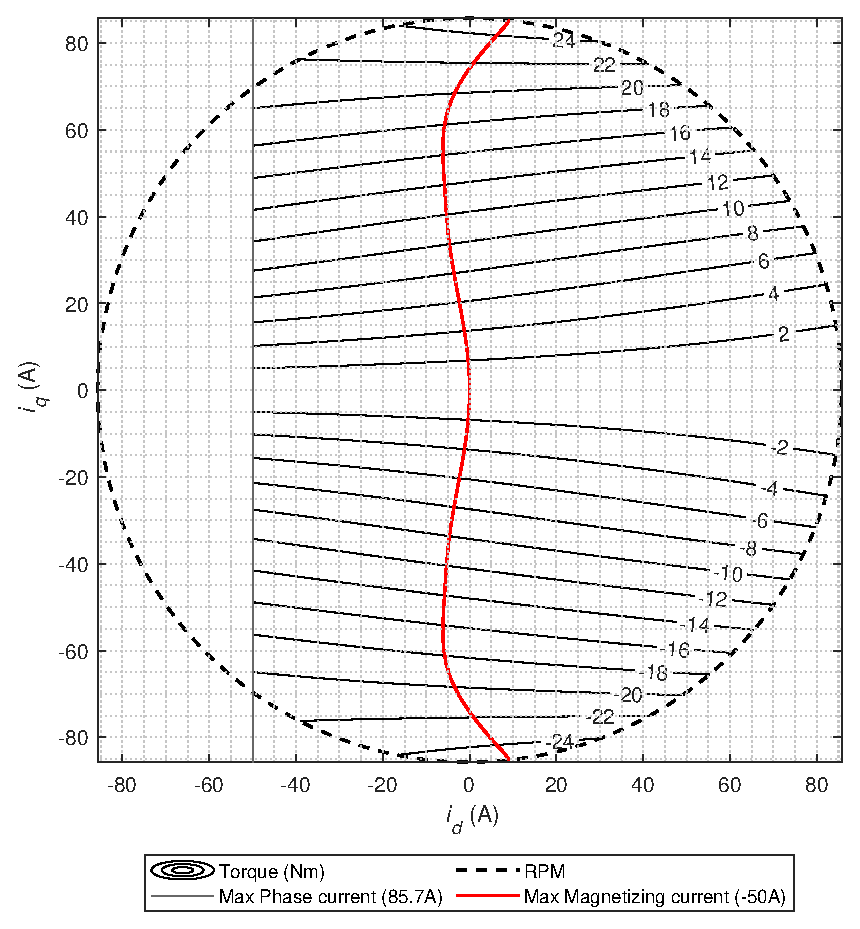
\includegraphics[width=0.6\textwidth]{Figures/Torque_MTPA_simple.eps}
	\caption[Maximum Torque per Ampere curve without constraints.]{Maximum Torque per Ampere curve without constraints.}
	\label{fig:mtpa_simple} %chktex 24
\end{figure}

\subsection{Contraints with limited input voltage}

While direct, the presented approach does not account for voltage limitations, meaning that when the rotor speed increases the back emf becomes large enough to limit the current operation points. To account for that the voltage constraint must be defined.

If the current is assumed to be constant, \Cref{eq:motor_with_inductances_no_derivative} can be rearranged to calculate the maximum current for a given voltage and velocity as in \Cref{eq:voltage_constraint_model}, with the voltage constraint defined in \Cref{eq:voltage_constraint_vdc}.
% \begin{subequations}
% 	\begin{equation}
% 		0 =u_d -r i_d +\omega_e L_q i_q
% 	\end{equation}
% 	\begin{equation}
% 		0 = u_q -r i_q - \omega_e (L_d i_d +\psi_{PM})
% 	\end{equation}
% \end{subequations}

\begin{subequations}
	\begin{equation}
		u_d = r i_d -\omega_e L_q i_q
	\end{equation}
	\begin{equation}
		u_q =  r i_q + \omega_e (L_d i_d +\psi_{PM})
	\end{equation}
    \label{eq:voltage_constraint_model} %chktex 24
\end{subequations}
\begin{equation}
	\sqrt{u_d^2+u_q^2}\leq V_{DC}
    \label{eq:voltage_constraint_vdc} %chktex 24
\end{equation}

Subjecting \Cref{eq:voltage_constraint_model} to \Cref{eq:voltage_constraint_vdc} an ellipse equation is obtained, where the center is defined by the rotor speed and the flux linkage, while the radius is defined by the DC link voltage and the resistance. The ellipse is defined as in \Cref{eq:voltage_ellipse}.
% \begin{equation}
% 	\psi_d = L_di_d + \psi_{PM}
% \end{equation}
% \begin{equation}
% 	\psi_q = L_qi_q
% \end{equation}

\begin{equation}
	{(r i_d -\omega_e \psi_q)}^2 + {(r i_q + \omega_e \psi^*_d)}^2\leq V_{DC}^2
	\label{eq:voltage_ellipse} %chktex 24
\end{equation}

Here $\psi^*_d = L_d i_d + \psi_{PM}$ and $\psi_q = L_q i_q$. Note that this ellipse size dynamically changes depending on the instantaneous rotor velocity and DC link voltage.

Using the ellipse as a constraint, \Cref{eq:mtpa_problem} can be rewritten as in \Cref{eq:mtpa_problem_with_voltage_constraint}, where the speed and DC link voltage are known.
\begin{equation}
	\begin{aligned}
		\min_{i_d,i_q} \quad & \sqrt{i_q^2 + i_d^2} \\
		\rm{s.t.}  \quad & T_{ref} = p\, i_q((L_d - L_q)i_d + \psi_{PM})\\
		               \quad & {(r i_d -\omega_e \psi_q)}^2 + {(r i_q + \omega_e \psi^*_d)}^2\leq V_{DC}^2            \\
	\end{aligned}
	\label{eq:mtpa_problem_with_voltage_constraint} %chktex 24
\end{equation}

This optimization problem was formulated on \textit{MATLAB} for several speeds and voltages. Some of the main cases are shown in \Cref{fig:mtpa_constrained}. On this graph, the iso-torque lines show the current combinations that yield the same torque, independent of the velocity or the voltage. The voltage ellipses are defined from the rotor velocity and the current DC link voltage, and they assume that the current is constant. The area contained by the ellipse is the feasible region at that speed and supply voltage. Steady-state operation at any point outside the ellipse would require a speed reduction or a voltage increase.
% figures \ref{fig:mtpa_Constrained_420}, \ref{fig:mtpa_Constrained_540}, and \ref{fig:mtpa_Constrained_588}.
% \begin{figure}[H]
% 	\centering
% 	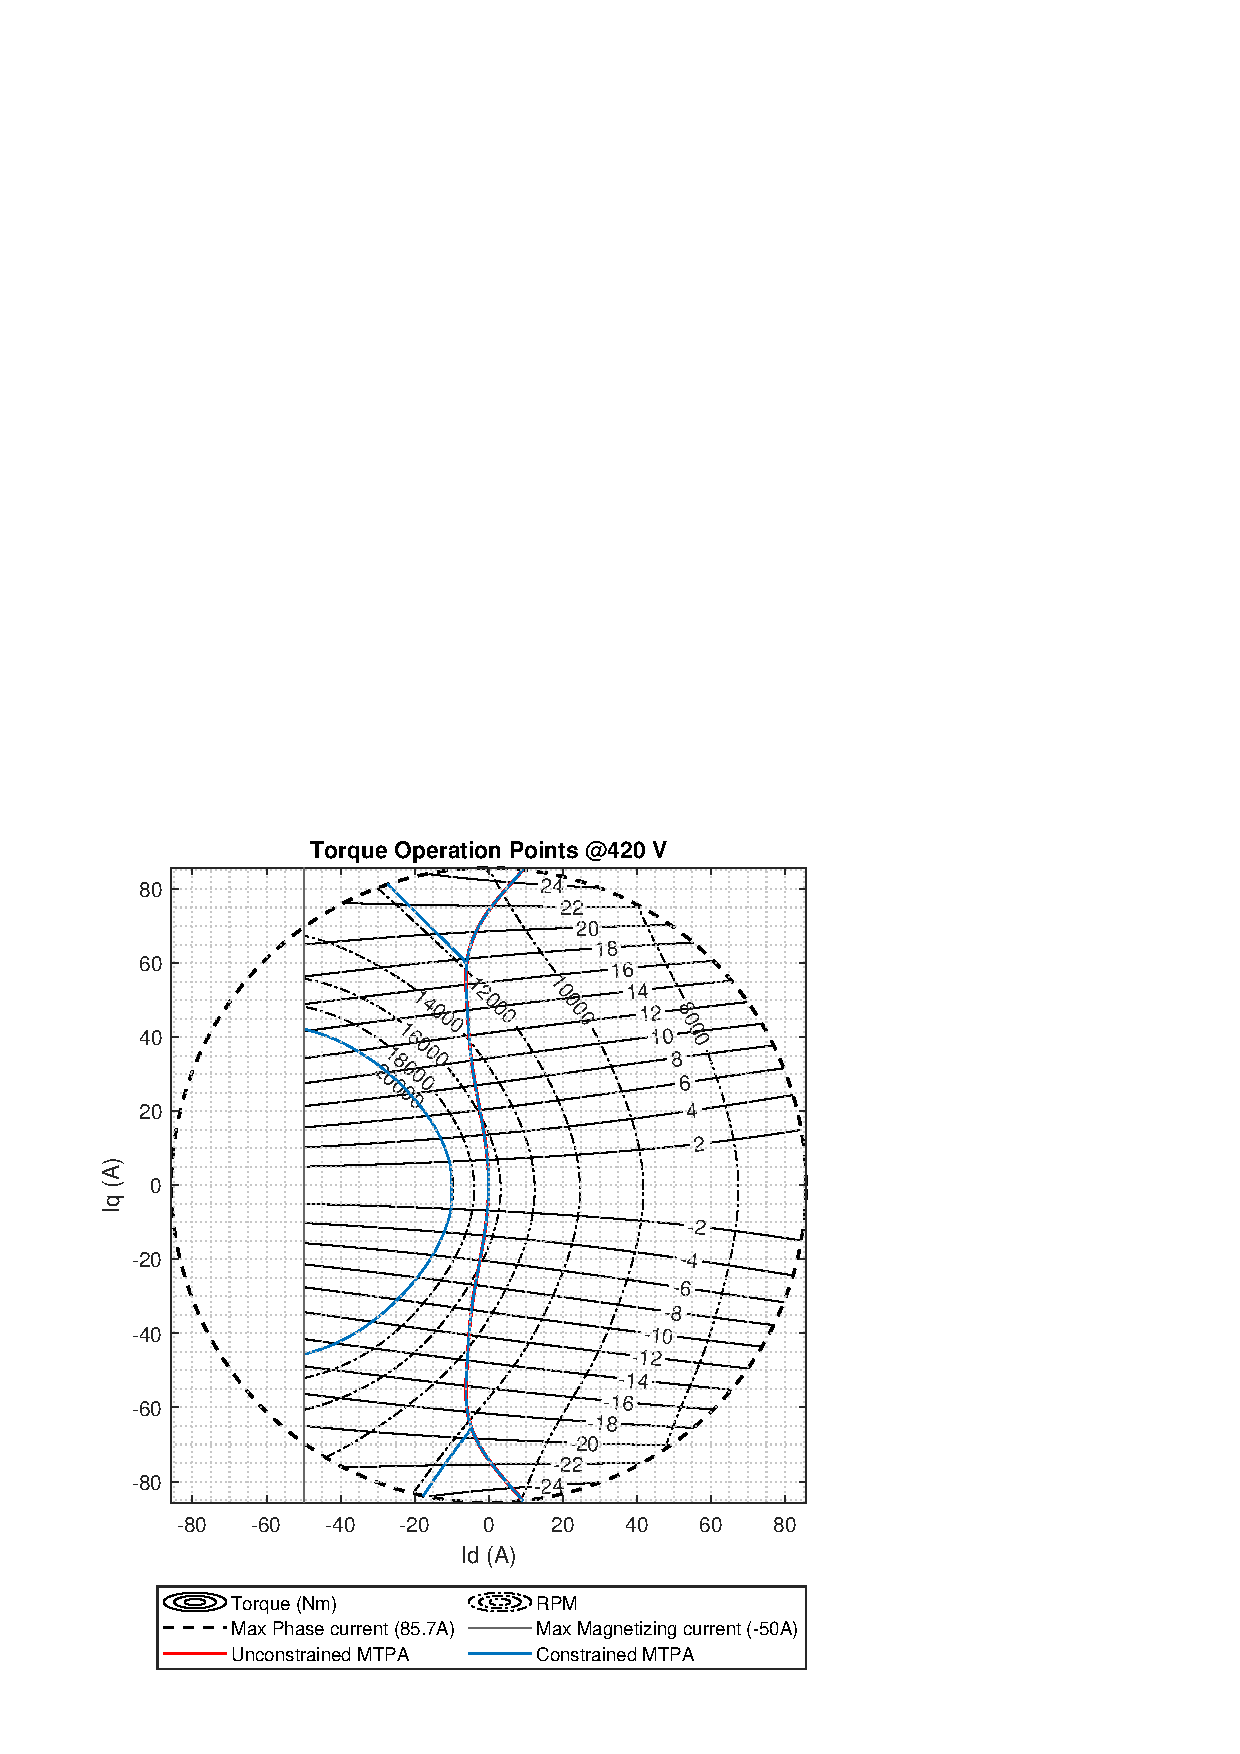
\includegraphics[width=0.65\textwidth]{Figures/Motor_map@420V.png}
% 	\caption[Maximum Torque per Ampere curve constrained @420V.]{Maximum Torque per Ampere curve constrained @420V}
% 	\label{fig:mtpa_Constrained_420} %chktex 24
% \end{figure}
% \begin{figure}[H]
% 	\centering
% 	\includegraphics[width=0.65\textwidth]{Figures/Motor_map@540V.png}
% 	\caption[Maximum Torque per Ampere curve constrained @540V.]{Maximum Torque per Ampere curve constrained @540V}
% 	\label{fig:mtpa_Constrained_540} %chktex 24
% \end{figure}
% \begin{figure}[H]
% 	\centering
% 	\includegraphics[width=0.65\textwidth]{Figures/Motor_map@588V.png}
% 	\caption[Maximum Torque per Ampere curve constrained @588V.]{Maximum Torque per Ampere curve constrained @588V}
% 	\label{fig:mtpa_Constrained_588} %chktex 24
% \end{figure}
\begin{figure}[!htb]
	\begin{subfigmatrix}{2}
		\subfigure[Minimum Voltage]{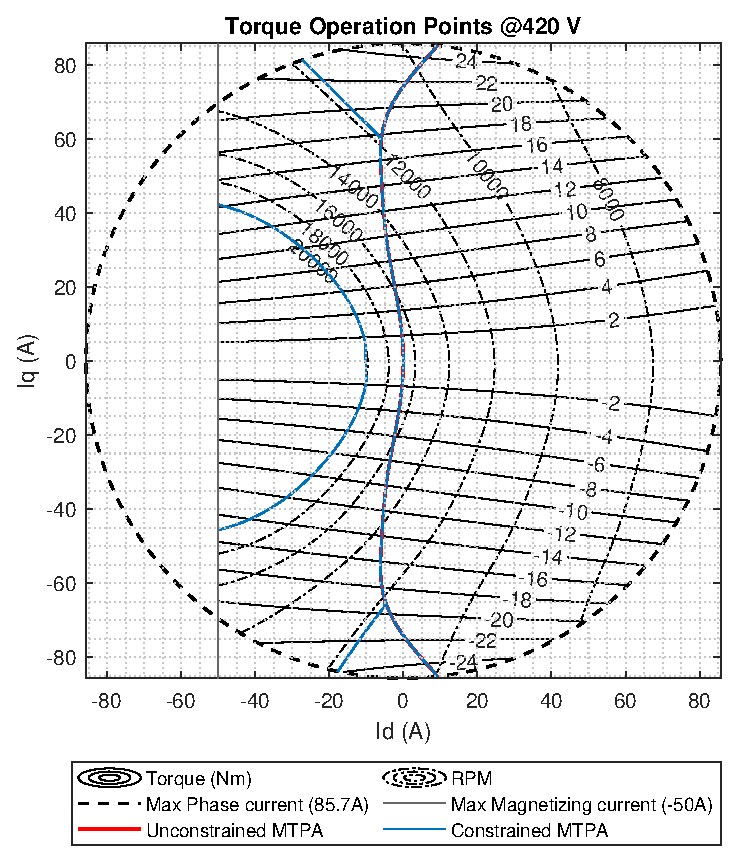
\includegraphics[width=0.49\linewidth]{Figures/Motor_map@420V}\label{fig:mtpa_Constrained_420}}
		\subfigure[Nominal Voltage]{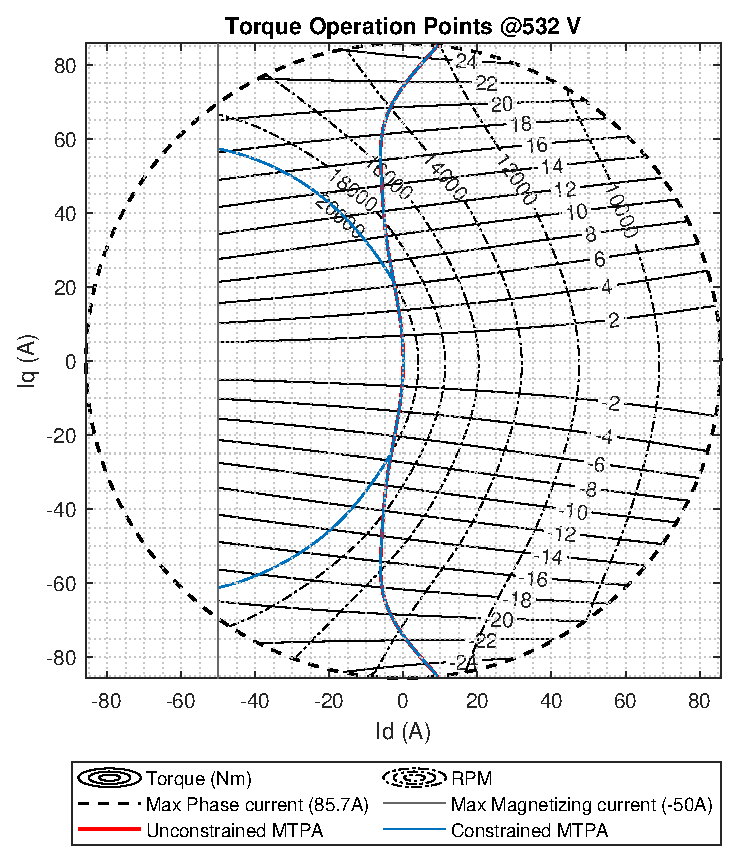
\includegraphics[width=0.49\linewidth]{Figures/Motor_map@532V}\label{fig:mtpa_Constrained_540}}
	\end{subfigmatrix}
	\begin{subfigmatrix}{1}
		\subfigure[Maximum Voltage]{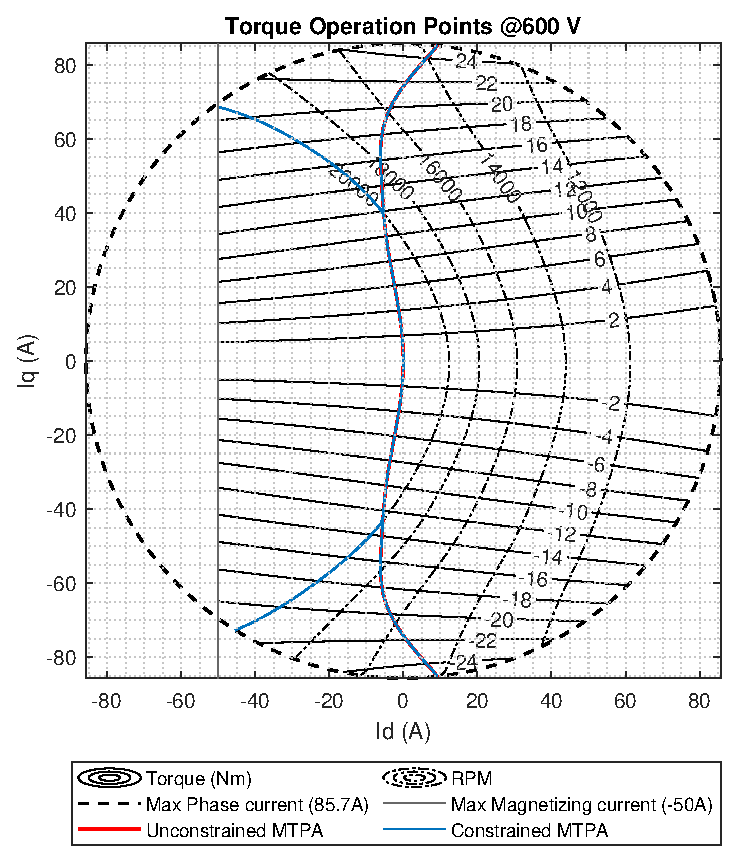
\includegraphics[width=0.49\linewidth]{Figures/Motor_map@600V}\label{fig:mtpa_Constrained_588}}
	\end{subfigmatrix}
	\caption{Constrained Maximum Torque per Ampere curve at minimum, nominal, and maximum voltages. Reference currents are shown for 0, 13000 and 2000 RPMs.}
	\label{fig:mtpa_constrained}%chktex 24
\end{figure}

Note that while the torque map is symmetrical relating to the $i_d$ axis, the voltage ellipse is not, it has been rotated slightly in an anti-clockwise direction. This rotation is due to the resistance of the phases that when the machine is working as a motor, reduce the total available voltage to fight the back EMF.\@ If the phase resistance is low the ellipse becomes aligned with the $i_d$ axis. Another important remark is the center of the voltage ellipse, as the AMK motor has permanent magnets with strong flux linkage the ellipse center is shifted farther away from the origin, but in a reluctance machine, the center would be at the origin, the same as the torque. Special cases appear when the ellipse center is inside the feasible current region, as the voltage-limited speed goes to infinity. An important location in this graph is the motor characteristic point, which can be easily located as being the place where the maximum phase current circumference yields the higher torque. The speed at this point is the motor's characteristic speed, and if the graph is created for the motor's nominal voltage, that becomes also the nominal speed of the motor. This point is important as any further increase in speed will result in a reduction in the maximum motor torque.

Figure~\ref{fig:mtpa_constrained} clearly shows that the optimal current reference is the \gls{mtpa} while the velocity and voltages allow it, and after that, the voltage ellipse becomes the best alternative. It is important to understand that the voltage constraint is dependent on the combination of DC Link voltage and rotor speed, when the voltage increases the ellipse for a given speed expands, allowing further operation on the unconstrained \gls{mtpa} line. This not only increases efficiency (as it produces the same torque with less current) but also improves performance, pushing the motor characteristic point further on the torque vs rpm diagram. 

Some processing is still needed to account for points outside of the feasible region, but the presented graphs can be used as a motor map,  where given the current DC Link voltage, motor speed, and desired torque, it returns the reference currents to optimally reach the torque reference. This can also be expanded to include temperature effects. 

\subsection{Inductance Curves}
\label{section:inductance_curves_current_reference}

The inductance curves used to generate the motor maps presented in \Cref{section:Current_references} were obtained from a spreadsheet provided by the manufacturer that contained simulation data. The inductances computed from it are presented in \Cref{fig:inductance_manufacturer}. However, for the sake of completeness, the current reference curves generated from the inductance values obtained through characterization (\Cref{fig:inductances_method_2}) are included in the \Cref{chapter:appendix_current_reference}. This was necessary because a working testbench with stable control was needed to properly characterize the inductances. This characterization was completed after the implementation of the control in the experimental setup. Unfortunately, shortly after, testbench limitations impeded further testing. Consequently, the maps generated using the characterization inductance curves were not tested experimentally.

\begin{figure}[!htb]
	\centering
	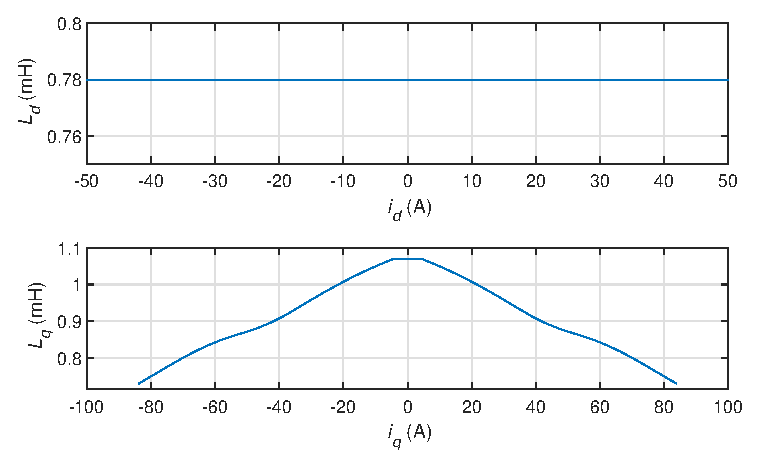
\includegraphics[width=0.7\textwidth]{Figures/ldq_manufacturer.eps}
	\caption[Manufacturer inductance curves.]{Manufacturer inductance curves.}
	\label{fig:inductance_manufacturer} %chktex 24
\end{figure}

Note that replacing the manufacturer tables with the characterized inductance curves from the appendix should not have a significant impact on the controller performance, only affecting the current references passed to the controller. The process to generate the current references and the controller structure remains the same despite the inductance curves.
%%%%%%%%%%%%%%%%%%%%%%%%%%%%%%%%%%%%%%%%%%%%%%%%%%%%%%%%%%%%%%%%%%%%%%%%
%                                                                      %
%     File: Load_Profile.tex	                                       %
%     Tex Master: Thesis.tex                                           %
%                                                                      %
%     Author: Israel Sother                                            %
%     Last modified: 27 May 2024                                       %
%                                                                      %
%%%%%%%%%%%%%%%%%%%%%%%%%%%%%%%%%%%%%%%%%%%%%%%%%%%%%%%%%%%%%%%%%%%%%%%%
\section{Load profile}
\label{section:03load_profile}
\vfill

To properly simulate the use case of the motor, a representative load profile must be defined. This profile will be used in the motor torque balance equations inside the simulations. To derive a representative load profile for the motor a car model is necessary. In this case, a simple one-dimensional point mass model is used in \Cref{eq:load_prof_initial}.
\begin{equation}
	\left(m_{car}+m_{wheel\,equivalent}\right)a_x = F_{motor}\eta_{transm}-F_{rolling\,resistance}-F_{drag}
	\label{eq:load_prof_initial}
\end{equation}
Where the rolling resistance is a constant force that depends on the rolling resistance coefficient and the weight of the car (\Cref{eq:rolling_resistance}), the losses are neglected, and the aerodynamic drag is calculated as in \Cref{eq:drag_force}.
\begin{equation}
	F_{drag} = 0.5\rho C_{d} A_{r} v^2
	\label{eq:drag_force}
\end{equation}
\begin{equation}
	F_{rolling\,resistance} = C_{r} m_{car} g
	\label{eq:rolling_resistance}
\end{equation}

To calculate the inertia seen by the motor, an equivalent rotational inertia must be computed. To do that, the energy stored in the rotating parts and on the car is equated with the equivalent inertia as shown in \Cref{eq:iner_equivalent0}.
\begin{equation}
	\frac{1}{2}J_{eq}\omega^2 = \frac{1}{2}m_{car}v^2 + \frac{1}{2}J_{wheels}\omega^2_{wheels}
	\label{eq:iner_equivalent0}
\end{equation}
Assuming a no slip condition, the car velocity can be replaced by $v = \omega_{wheels}r_{tire}$, which gives \Cref{eq:iner_equivalent1}.
\begin{equation}
	\frac{1}{2}J_{eq}\omega^2 = \frac{1}{2}m_{car}(\omega_{wheels}r_{tire})^2 + \frac{1}{2}J_{wheels}\omega_{wheels}^2
	\label{eq:iner_equivalent1}
\end{equation}
Knwoing the transmission gear ratio the wheel velocity is replaced by its equivalent in the motor, as in $\omega_{wheels} = \frac{\omega}{G_r}r_{tire}$, yielding \Cref{eq:iner_equivalent2}.
\begin{equation}
	\frac{1}{2}J_{eq}\omega^2 = \frac{1}{2}m_{car}\left(\frac{\omega}{G_r}r_{tire}\right)^2 + \frac{1}{2}J_{wheels}\left(\frac{\omega}{G_r}\right)^2
	\label{eq:iner_equivalent2}
\end{equation}
Rearranging to solve for $J_{eq}$ results in \Cref{eq:iner_equivalent}.
% \begin{equation}
% 	\frac{1}{2}J_{eq}\omega^2 = \frac{1}{2}\left(\frac{m_{car}r_{tire}^2}{{Gr^2}} + \frac{J_{wheels}}{Gr^2}\right) \omega^2
% 	\label{eq:iner_equivalent3}
% \end{equation}
\begin{equation}
	J_{eq} = \frac{m_{car}r_{tire}^2 + J_{wheels}}{G_r^2}
	\label{eq:iner_equivalent}
\end{equation}

From experimental tests with previous prototypes, a good rule of thumb is that when accelerating, only one-third of the power can be applied at the front axle, while the rear axle receives two-thirds. Ideally, a weight transfer function would be used, but to simplify the equations the constant distribution will be used. Thus the equivalent rotational inertia at each motor is on \Cref{eq:motor_iner_equivalent}, where \Cref{eq:motor_iner_equivalent_front} is for the front axle motors, and \Cref{eq:motor_iner_equivalent_rear} for the rear. This diference is to account the approximated load transfer when the vehicle is accelerating.

\vspace{0.5cm}
\begin{subequations}
	\centering
	\begin{minipage}{.47\linewidth}
		\begin{equation}
			J_{f_{eq}} = 2\frac{m_{car}r_{tire}^2 + 6\;J_{wheels}}{12\;G_r^2}
			\label{eq:motor_iner_equivalent_front}
		\end{equation}
	\end{minipage}
	\begin{minipage}{.47\linewidth}
		\begin{equation}
			J_{r_{eq}} = 2\frac{m_{car}r_{tire}^2 + 3\;J_{wheels}}{6\;G_r^2}
			\label{eq:motor_iner_equivalent_rear}
		\end{equation}
	\end{minipage}
	\label{eq:motor_iner_equivalent}
\end{subequations}
\vspace{0.5cm}

Combining the equations, a torque profile for each axle is defined in \Cref{eq:load_profile}. Where the second term represents the load torque, at a given car state, and $\frac{J_{f_{eq}}}{2}$ is the equivalent inertia.

\begin{subequations}
	\begin{equation}
		\frac{J_{f_{eq}}}{2}\dot{\omega} = T_{motor}\eta_{transm}  - \frac{\left(F_{rolling\,resistance}+F_{drag}\right)r_{tire}}{6\;G_r}
	\end{equation}
	\begin{equation}
		\frac{J_{r_{eq}}}{2}\dot{\omega} = T_{motor}\eta_{transm}  - \frac{\left(F_{rolling\,resistance}+F_{drag}\right)r_{tire}}{3\;G_r}
	\end{equation}
	\label{eq:load_profile}
\end{subequations}
%%%%%%%%%%%%%%%%%%%%%%%%%%%%%%%%%%%%%%%%%%%%%%%%%%%%%%%%%%%%%%%%%%%%%%%%
%                                                                      %
%     File: Proposed_control.tex                                  	   %
%     Tex Master: Thesis.tex                                           %
%                                                                      %
%     Author: Israel Sother                                            %
%     Last modified: 27 May 2024                                       %
%                                                                      %
%%%%%%%%%%%%%%%%%%%%%%%%%%%%%%%%%%%%%%%%%%%%%%%%%%%%%%%%%%%%%%%%%%%%%%%%
\section{Control Methods Development}
\label{section:Control Methods Development}%chktex 24

In this section some of the main \glspl{mpc} used on the power converters field are developed. At the end of the section, the proposed control strategy is presented. The methods compared with the manufacturer's \gls{foc} are:
\begin{itemize}
	\item Finite Set \gls{mpc}
	\item Finite Set with null vector \gls{mpc}
	\item Non-Linear Continuous Set \gls{mpc}
	\item \acrfull{rush}
\end{itemize}
All those methods rely on the line current and rotor position encoder data to estimate the currents in the dq0 frame. The DC Link voltage is also measured to account for battery voltage fluctuation. The control strategy is then applied to the motor model to predict the next time step values. This processed data is refreshed at each time step to be utilized by the selected control strategy.
Although it is possible to use multiple horizon prediction steps, to keep the computational cost low, and maintain high switching frequencies, all the proposed methods use a horizon of only 1 discretized time step. 
% This is later verified as not having an expressive take on performance as the system is fast enough so that the dynamics are well represented with only one timestep.

Some of these control methods depend on a cost function definition to choose the best control action. The control action that minimizes this cost function is then applied to the system.
\begin {subequations}
	\begin{equation}
	\begin{aligned}
		\mathcal{J} =  s_1 \left(\frac{i_{d_{ref}}-i_{d_{k+1}}}{i_{d_{ref}}}\right)^2 + s_2 \left(\frac{i_{q_{ref}}-i_{q_{k+1}}}{i_{q_{ref}}}\right)^2 + \mathcal{C}_{soft}
	\end{aligned}
	\label{eq:cost_mpc}
	\end{equation}
	\begin{equation}
	\mathcal{C}_{soft} = s_3 \max\left(0,\sqrt{i_{d_{k+1}}^2 + i_{q_{k+1}}^2} - \sqrt{\frac{2}{3}} i_{line max}\right) + s_4 \max\left(0,\sqrt{u_{d_{k+1}}^2+u_{q_{k+1}}^2}-V_{DC}\right)
	\label{eq:soft_constraints_mpc}
	\end{equation}
\end{subequations}
The cost function shown in \Cref{eq:cost_mpc} is composed of the error between the reference and the predicted values of the currents, and a soft constraint that penalizes the system for exceeding the maximum line current or the DC link voltage while some gains $s_x$ are used to adjust the priorities. The soft constraint is defined in \Cref{eq:soft_constraints_mpc}.

\subsection{Finite Set MPC}
In a \gls{fsmpc} each of the basic vectors defined on \Cref{table:space_vector} are applied to \Cref{eq:motor_backward_euler_matrix} using the current measured data, resulting in different predictions for the next time step values. A cost function that compares the torque and currents (to account for \gls{mtpa}) with the references, is then evaluated for each of those predictions. The vector with the lowest cost is then applied at the next time step, as shown in \Cref{fig:FSMPC_Diagram}.
\begin{figure}[!htb]
	\centering
	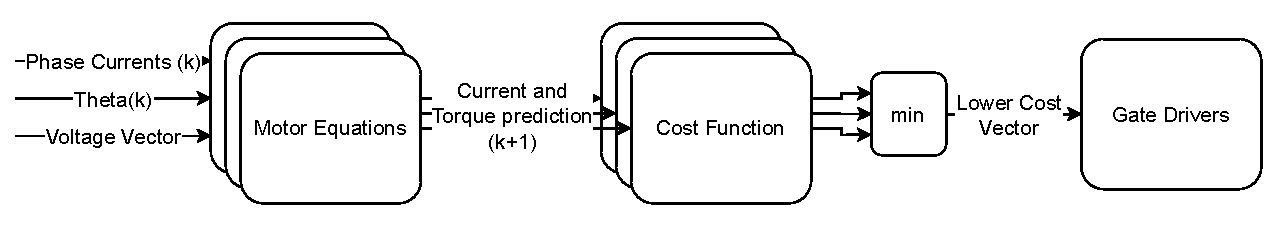
\includegraphics[width=0.8\textwidth]{Figures/FSMPC.pdf}
	\caption[FSMPC Diagram.]{FSMPC Diagram.}
	\label{fig:FSMPC_Diagram}%chktex 24
\end{figure}

\subsection{Finite Set with Null Vector MPC}

Although effective, the simple Finite Set \gls{mpc} can incur heavy torque ripple, due to its limited options on which vector can be applied. That behavior can be exacerbated by low power operation points, where the active vectors result in a bigger percentual change in currents. This problem can be mitigated by introducing the possibility of sharing the sample time between the chosen active vector and a null vector. Such an approach allows the control to apply vectors that point in the direction of the native ones but have smaller amplitude.

This addition of a null vector comes with the problem of now having virtually infinite vector options (depending on the \gls{pwm} resolution), but that can be solved with some approximations. This method begins as the previous one, where each of the 7 possible vectors is applied to the motor model, but before passing those results for the cost function the predicted torque is compared with the reference. If a crossing is detected, meaning the values $T_{ref} - T_{e(k)}$ and $T_{ref} - T_{e(k+1)}$ have different signals the algorithm assumes that the ideal vector has a smaller amplitude, thus computes a ratio of active vector time and null vector time. To calculate such a ratio an approximation was made that, given the short sample time, the complete system is assumed to behave linearly during that period. If the system behaves linearly, the currents and torque for a combination of null and active vectors will also be a linear combination of the individual values for each vector multiplied by its application time. This approximation is shown in \Cref{eq:linear_combination,eq:linear_combination_torque}, where $d$ is the duty cicle value for a given vector, and the subscripts $_{act}$ and $_n$ represents the active and null vectors respectively.

\begin{equation}
	i_x = i_{act} d_{act} + i_n d_n
	\label{eq:linear_combination}
\end{equation}
\begin{equation}
	T_x = T_{act} d_{act} + T_n d_n = T_{act} d_{act} + T_n - T_n d_{act}
	\label{eq:linear_combination_torque}
\end{equation}

With that property, and knowing that $d_{act} + d_n = 1$ the duty cycle for the active vector is calculated as shown in \Cref{eq:duty_cycle}.

\begin{equation}
	d_{act} = \frac{T_{ref} - T_n}{T_{act}-T_n}
	\label{eq:duty_cycle}
\end{equation}


Given the duty cycle, the predictions are updated and passed to the cost function, which chooses the best combination of active and null vectors. A diagram of this method is shown in \Cref{fig:FSMPC_null_Diagram}.

\begin{figure}[!htb]
	\centering
	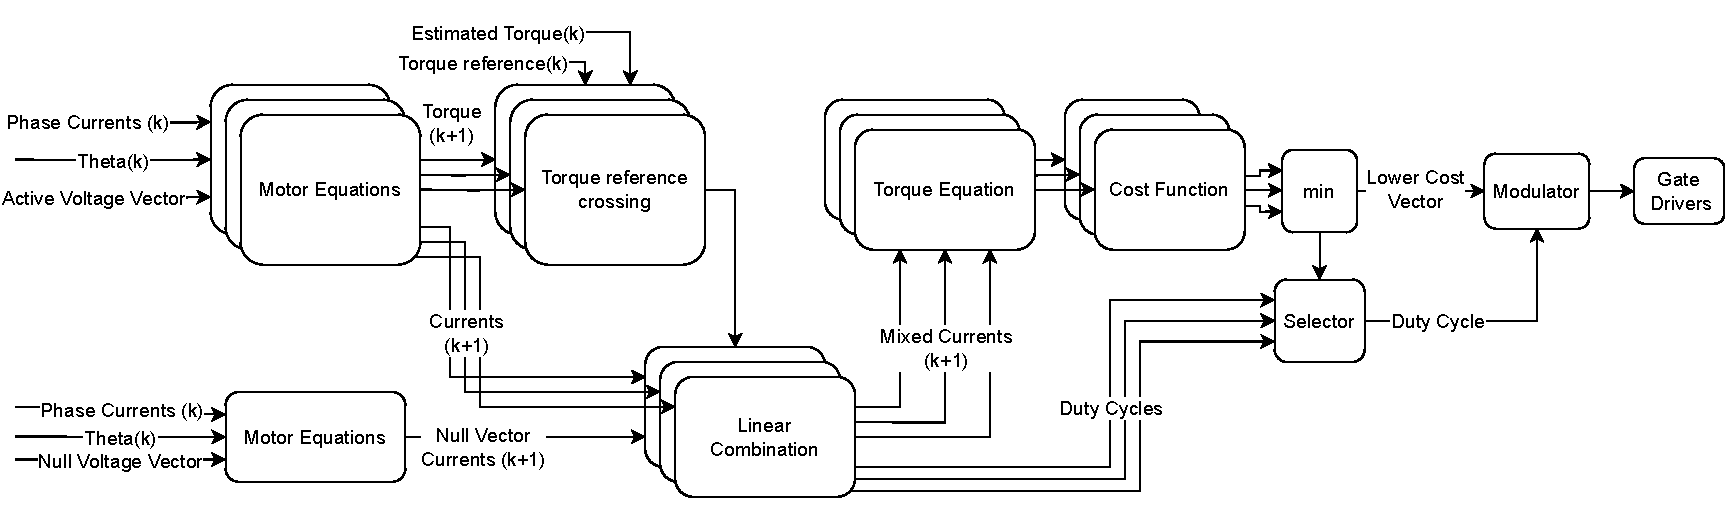
\includegraphics[width=1\textwidth]{Figures/FSMPC_null_vector.pdf}
	\caption[Finite Set with Null Vector MPC Diagram.]{Finite Set with Null Vector MPC Diagram.}
	\label{fig:FSMPC_null_Diagram}%chktex 24
\end{figure}

\subsection{Non-Linear Continuous Set MPC}

In the continuous set \glspl{mpc} the control action is not limited to a finite set of vectors, but it is assumed that any vector attainable by a defined modulation technique is available. This increases the complexity of the control, as the control action locus becomes infinite.
 This approach is very similar to the most common approach of \gls{mpc} used in other fields that are not power systems. It takes an implicit approach, where the motor model shown in \Cref{eq:motor_backward_euler_matrix} is combined with an optimization solver that numerically finds the best control action. This \gls{mpc} technique has the advantage of easy constraints implementation while having the benefits of a continuous set controller. This advantage comes at the cost of largely increased computational time, as it needs to evaluate the model equation several times to find the optimal voltage vector that fulfills the constraints. This additional complexity can often be prohibitive for power systems where a fast-acting control is needed. The diagram of this method is shown in \Cref{fig:implicit_csmpc_diagram}.

\begin{figure}[!htb]
	\centering
	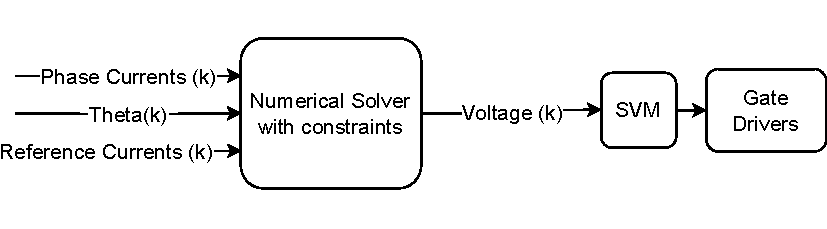
\includegraphics[width=0.65\textwidth]{Figures/Implicit_CSMPC.pdf}
	\caption[Implicit Continuous Set MPC Diagram.]{Implicit Continuous Set MPC Diagram.}
	\label{fig:implicit_csmpc_diagram}%chktex 24
\end{figure}

\subsection{RUSH MPC}

One of the advantages of the approximations made in the discretization process is that even though the matrices change in time, for a given moment the system is linear, and as such an inverse dynamic can be derived. So, if in \Cref{eq:motor_backward_euler_matrix} the currents on the next step are replaced by a reference for the current vector, the necessary applied voltage can be calculated in real-time. This is done by \Cref{eq:Vdq}.

\begin{equation}
	\begin{aligned}
		\begin{bmatrix}
			u_{d(k+1)} \\
			u_{q(k+1)} \\
		\end{bmatrix}
		=
		\begin{bmatrix}
			\frac{h}{hr+L_{d(i_d(k))}} & 0                          \\
			0                          & \frac{h}{hr+L_{q(i_q(k))}} \\
		\end{bmatrix}^{-1} \\
		\left(
		\begin{bmatrix}
				1                                                    & -h\frac{\omega_{e(k)}L_{q(i_q(k))}}{hr+L_{d(i_d(k))}} \\
				h\frac{\omega_{e(k)}L_{d(i_d(k))}}{hr+L_{q(i_q(k))}} & 1                                                     \\
			\end{bmatrix}
		\begin{bmatrix}
				i_{d_{ref}} \\
				i_{q_{ref}} \\
			\end{bmatrix}
		-
		\begin{bmatrix}
				\frac{L_{d(i_d(k))}}{hr+L_{d(i_d(k))}} & 0                                      \\
				0                                      & \frac{L_{q(i_q(k))}}{hr+L_{q(i_q(k))}} \\
			\end{bmatrix}
		\begin{bmatrix}
				i_{d(k)} \\
				i_{q(k)} \\
			\end{bmatrix}
		-
		\begin{bmatrix}
				0                                                 \\
				-h\frac{\omega_{e(k)}\psi_{PM}}{hr+L_{q(i_q(k))}} \\
			\end{bmatrix}
		\right)
	\end{aligned}
	\label{eq:Vdq}
\end{equation}

This approach is commonly used in linear unconstrained \glspl{mpc} to improve computation times, where a control law is precomputed and stored in memory. But in the presented case there is an important constraint that is not accounted for in the previous equation. When very short time steps are used, and there is a big reference change, the necessary voltage to achieve the target on just one discrete time step can be very high. This would lead to problems, like distortions due to overmodulation or not being able to reach the desired voltages. The solution to this problem is to saturate the voltage vector. Some authors have suggested saturating based on the closest possible vector~\cite{Fernando:fast_predictive:2013}, in this work, the saturation only limits the vector amplitude to match the DC-link voltage, maintaining the desired vector angle as shown in \Cref{eq:Vdq_saturation}.
\begin{subequations}
	\begin{equation}
			\gamma = arctg\left(\frac{u_{d(k+1)}}{u_{q(k+1)}}\right)
	\end{equation}
	\begin{equation}
		u_{sat_{d(k+1)}} = \min\left(u_{d(k+1)}\;,\; V_{DC}\cos(\gamma)\right)
	\end{equation}
	\begin{equation}
		u_{sat_{q(k+1)}} = \min\left(u_{q(k+1)}\;,\; V_{DC}\sin(\gamma)\right)
	\end{equation}
	\label{eq:Vdq_saturation}
\end{subequations}

\begin{figure}[!htb]
	\centering
	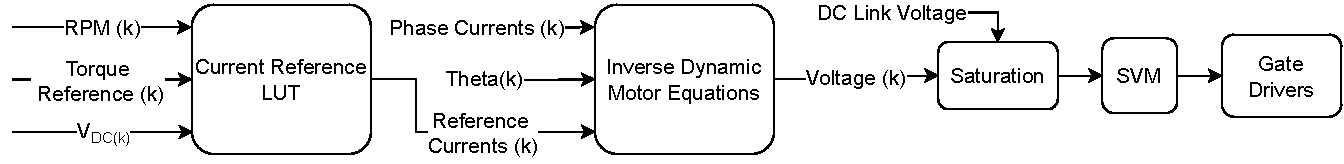
\includegraphics[width=1\textwidth]{Figures/Explicit_CSMPC.pdf}
	\caption[Explicit Continuous Set MPC Diagram.]{Explicit Continuous Set MPC Diagram.}
	\label{fig:explicit_csmpc_diagram}%chktex 24
\end{figure}

This method greatly reduces the time taken to compute the control action, as instead of trying 7 different possible inputs (or more) it just calculates one time the necessary voltage and clamps it to the attainable values. As this control uses a continuous set, those values are then forwarded to a \gls{svm} system to modulate the \gls{pwm} signals. The diagram of this method is shown in \Cref{fig:explicit_csmpc_diagram}.


%%%%%%%%%%%%%%%%%%%%%%%%%%%%%%%%%%%%%%%%%%%%%%%%%%%%%%%%%%%%%%%%%%%%%%%%
%                                                                      %
%     File: Horizon_extension.tex                                      %
%     Tex Master: Thesis.tex                                           %
%                                                                      %
%     Author: Israel Sother                                            %
%     Last modified: 27 May 2024                                       %
%                                                                      %
%%%%%%%%%%%%%%%%%%%%%%%%%%%%%%%%%%%%%%%%%%%%%%%%%%%%%%%%%%%%%%%%%%%%%%%%
\subsubsection{Horizon Extension}
\label{section:Horizon Extension}%chktex 24

A previously overlooked problem is the compensation of the computational time, as the acquisition and control calculations cannot be done instantly their delay needs to be compensated. The strategy adopted here is to use the motor model equations \Cref{eq:motor_backward_euler_matrix} coupled with the previously calculated control action to predict the system state in the next time step, this is called horizon extension. Usually, this is done in a fixed timestep manner, where the predictive controllers instead of picking the control action for $k$ in the timestep $k$, pick the control action for $k+1$ in the timestep $k$, as shown in \Cref{eq:horizon_default} where $x$ represent the currents, $u$ is the voltage vector, $A$, $B$, $C$, and $D$ are the matrices and vectors of the model in \Cref{eq:motor_backward_euler_matrix} and are all dependent on the prediction duration $h = \frac{1}{f_{sw}}$.
\begin{equation}
	x_{k+1} = A^{-1} \left (B x_k + C u_k + D\right )
	\label{eq:horizon_default}
\end{equation}

For this equation to work the system timeline needs to be as in \Cref{fig:horizon_default_timeline}, starting with taking the current and voltage measurements, followed by applying the voltage vectors calculated in $k-1$, then extending the horizon by one timestep, and calculating the voltage vector for the next timestep~\cite{Vazquez:MPC_uses:2014}.

\begin{figure}[!htb]
	\centering
	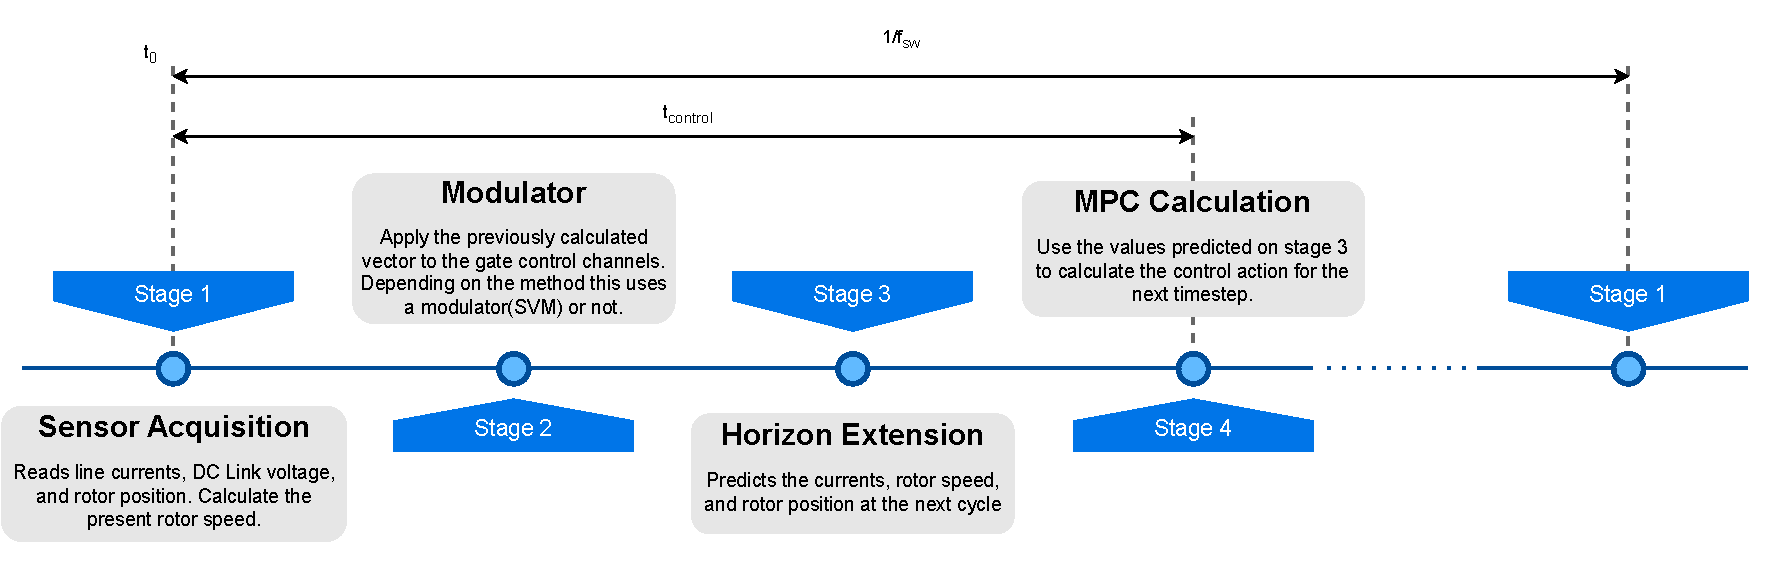
\includegraphics[width=1\textwidth]{Figures/Horizon Extension default Timeline.pdf}
	\caption[Horizon extension by one timestep.]{Horizon extension by one timestep.}
	\label{fig:horizon_default_timeline} %chktex 24
\end{figure}

This can be improved by only extending the horizon by the necessary time to compute the control action, this way the prediction error derived from model mismatch is reduced because the amount of time to predict is smaller. To do that the prediction duration is simply reduced to $h = t_{control}$, while the system timeline is shifted as in \Cref{fig:horizon_extend_timeline}. 


\begin{figure}[!htb]
	\centering
	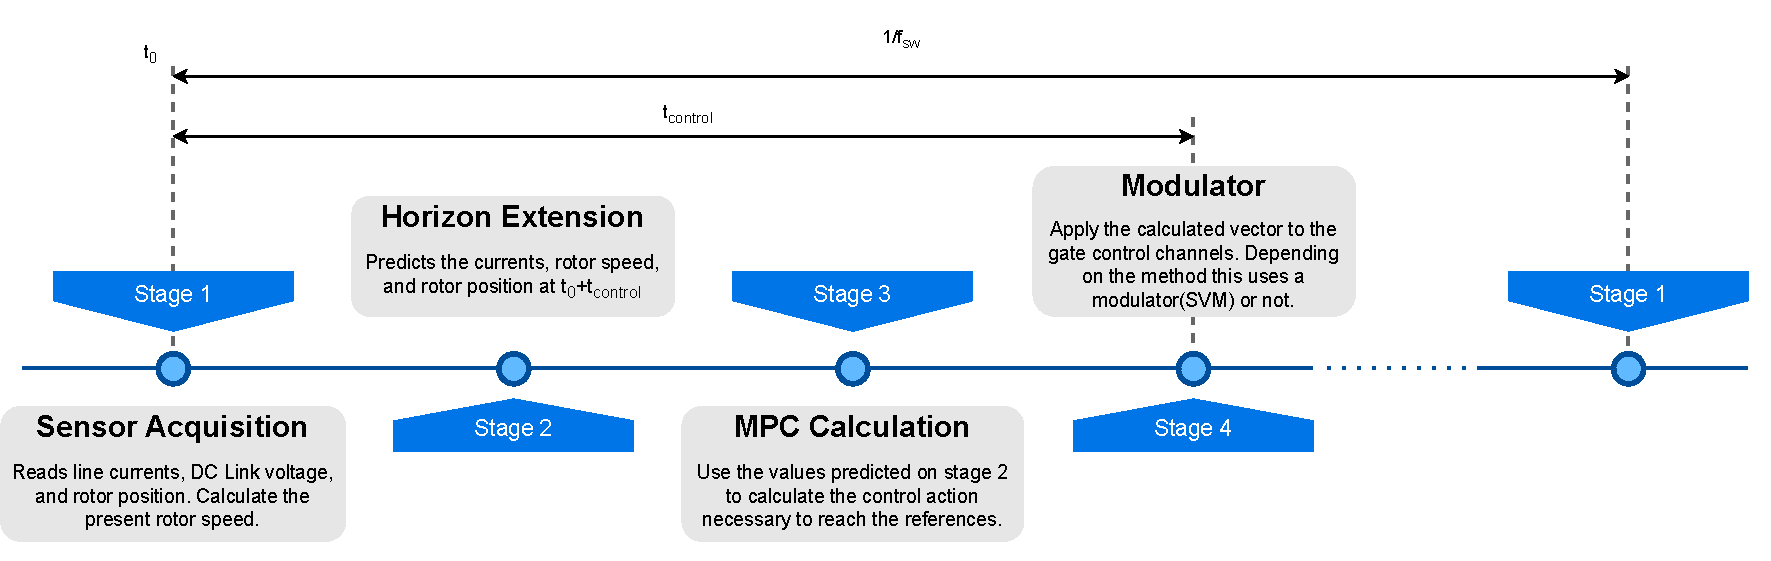
\includegraphics[width=1\textwidth]{Figures/Horizon Extension Timeline.pdf}
	\caption[Horizon Extension by control time.]{Horizon Extension by control time.}
	\label{fig:horizon_extend_timeline} %chktex 24
\end{figure}

The final control cycle starts with sensor acquisition, followed by horizon extension, and lastly the future control action computation. Note that this delay is not a problem with simulation in \textit{Simulink}, as it can instantly do the calculations, but it is good practice to simulate it with the proper delays to increase the similarity between simulation and experimental results.

A comparison of the different horizon extension methods is shown with example values in \Cref{fig:hor_comparison}. Here $\overline{\hat{i}_{dq}}$ represents the norm of the estimated dq current at the end of the horizon extension, $\overline{V_{dq}}$ is the norm of the dq voltage applied by the \gls{svm}, and $\overline{V^*_{dq}}$ is the norm of the computed dq voltage reference. The lines on the top represent the predicted and measured currents, while the lower lines are the voltages. Note that the markers in this figure are placed on the exact time the hardware finishes each computation, thus the delay between measurement, extension, and control calculation. The dashed voltage line represents the moment when the control action reference was computed, so in the regular horizon extension it is ahead of the applied control action as it needs to wait for the next \gls{svm} cycle to be applied. The ultra short horizon technique allows it to be applied as soon as it is computed, resulting in the computed reference and \gls{svm} applied voltages overlapping. Note that the use of a reduced horizon also improves the model mismatch, as the integration error is reduced shown by the reduced lag between the predicted and real currents in \Cref{fig:hor_comparison}.
\begin{figure}[!htb]
	\centering
	\begin{subfigmatrix}{2}
		\subfigure[Default Horizon Extension.]{
			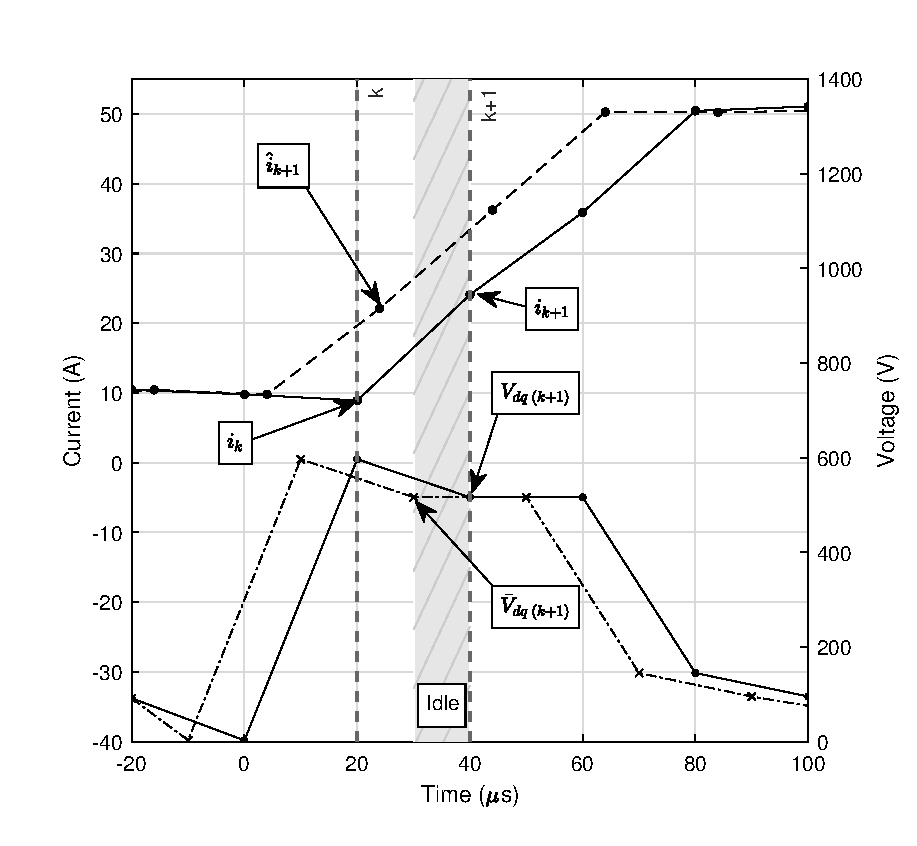
\includegraphics[width=.47\textwidth]{Figures/long_horizon.eps}
			\label{fig:normal_timeline}
		}
		\subfigure[Ultra Short Horizon Extension.]{
			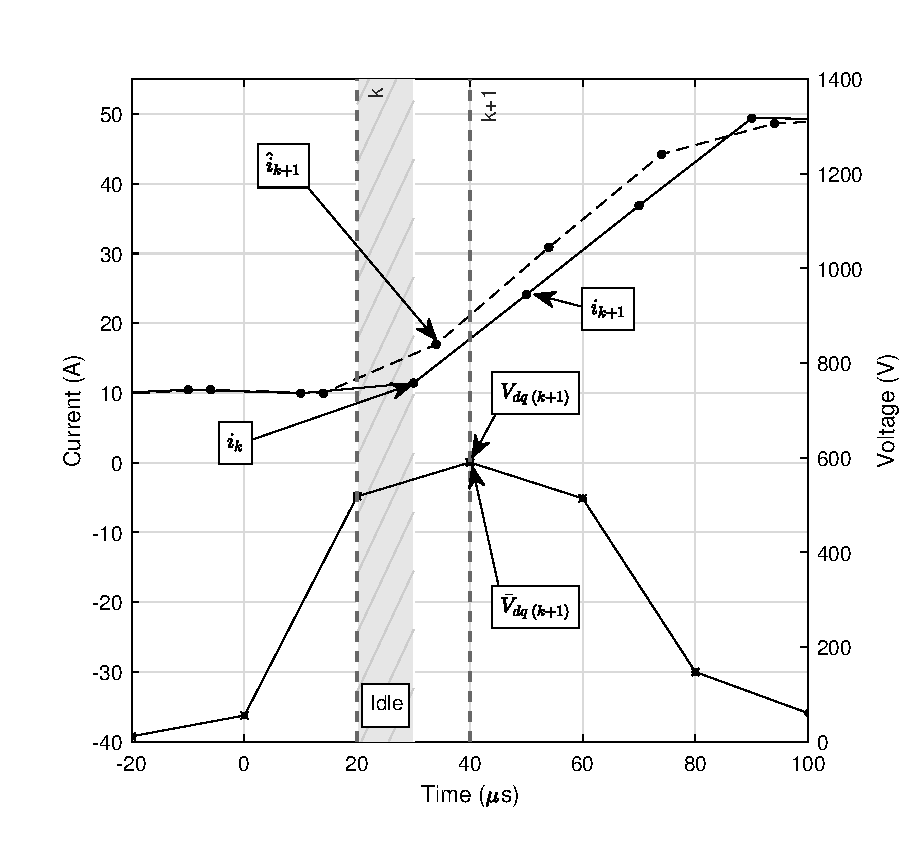
\includegraphics[width=.47\textwidth]{Figures/short_horizon.eps}
			\label{fig:USH_timeline}
		}
	\end{subfigmatrix}
	\caption{Horizon extension comparison, on top the measured and predicted voltages. The bottom lines are the computed control action and the applied control action}
	\label{fig:hor_comparison}
\end{figure}

The combination of explicitly solving the \gls{mpc} model equation with the hybrid horizon timestep approach, where the horizon extension has a shorter timestep than the controllable horizon is called \acrfull{rush}. It has the benefits of being a continuous set model predictive control, thus reducing the ripple, while being computationally efficient, as it is explicitly calculated, and reducing the prediction error due to model mismatch as it uses the reduced horizon extension technique.


\subsubsection{Speed Control}
\label{section:speed_control}%chktex 24

In the current architecture, the car has a slip controller that is responsible for limiting the wheels slip ratio. This controller is based on limiting the maximum (or minimum in the case of braking) speed that a wheel can have. In order to implement this it is necessary to have a rotor speed control. While this could be implemented directly on the \gls{mpc}, the speed dynamics are much slower than the current dynamics, and as such, it is possible to use a simpler control method. The proposed method is a PI controller that receives the rotor speed error and outputs a torque reference. This torque reference is then passed through a saturation which has the limits defined by the throttle and brake pedals, and the resultant torque is used as the input for the \gls{mpc} controllers. The saturation of torque is considered in the integral part of the PI, clamping it if the output is saturated. This structure is shown in \Cref{fig:speed_control_diagram}.

\begin{figure}[!htb]
	\centering
	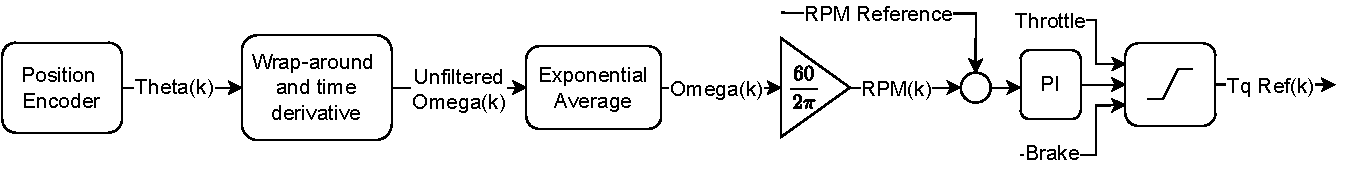
\includegraphics[width=1\textwidth]{Figures/Speed_control.pdf}
	\caption[Speed control diagram.]{Speed control diagram.}
	\label{fig:speed_control_diagram}%chktex 24
\end{figure}

Note that \Cref{fig:speed_control_diagram} also presents a calculation for the rotor speed, this is done by calculating the difference in rotor position between two-time steps and dividing by the sample time. As the rotor position encoder is absolute the position value has a wrap-around point, and thus to calculate the position time derivative an assumption is made that the rotor position does not change more than 180 degrees between two samples. This assumption is valid as the maximum speed of the motor is $20000 rpm$, which translates to $333 Hz$, and the sample time of the encoder is smaller than  $70\mu s$, meaning that the rotor can only move $8.4 \degree$ between samples. This value can increase in the case of a failure in the encoder, but the margin is large enough to accommodate eventual encoder failures. With the rotor position derivative calculated, exponential averaging is applied to smooth the signal and reduce noise, this is done by \Cref{eq:rotor_speed}, where $\alpha$ is the smoothing factor, that defines the weight of the past samples in the current average.

\begin{equation}
	\omega_{(k+1)} = \alpha \omega_{(k)} + (1-\alpha) \frac{\theta_{(k+1)} - \theta_{(k)}}{h}
	\label{eq:rotor_speed}
\end{equation}

A continuous approximation of the exponential moving average can be modeled as a transfer function of a first-order system, with a time constant defined by the smoothing factor $\alpha$, as shown in \Cref{eq:time_constant,eq:exp_moving_average}.


\begin{equation}
	\tau = \frac{-h}{\ln(\alpha)}
	\label{eq:time_constant}
\end{equation}
\begin{equation}
		\frac{\omega}{\omega_{unfiltered}} = \frac{\frac{1}{\tau}}{s+\frac{1}{\tau}}
	\label{eq:exp_moving_average}
\end{equation}

To define the speed controller gains, a simplified motor model was used. As the torque controller is much faster than the speed dynamic, it is assumed to be ideal, without delay. Thus, the speed is only dependant on the motor torque ($T_{e}$), mechanical losses ($T_{loss}$), the external load ($T_{loss}$), and the system inertia ($J$), as shown in \Cref{eq:speed_model}.

\begin{equation}
		\frac{d\omega_{unfiltered}}{dt} = \frac{T_e-T_{load} - T_{loss}}{J}
	\label{eq:speed_model}
\end{equation}

Using the Laplace transform the transfer function is given by \Cref{eq:speed_tf}.

\begin{equation}
		\frac{\omega_{unfiltered}}{T_e} = \frac{1}{J s}-\frac{T_{load} + T_{loss}}{J T_e s}
	\label{eq:speed_tf}
\end{equation}

Assuming the external load, and the mechanical losses as disturbances, the model can be reduced to a first-order system, shown in \Cref{eq:speed_tf_reduced}.

\begin{equation}
		\frac{\omega_{unfiltered}}{T_e} = \frac{1}{J s}
	\label{eq:speed_tf_reduced}
\end{equation}

Combining the motor model with the exponential moving average, a transfer function for the system can be derived, as shown in \Cref{eq:plant_speed_controller}.

\begin{equation}
		H(s) = \frac{\omega}{T_e} = \frac{1}{\tau J s^2+J s}
	\label{eq:plant_speed_controller}
\end{equation}

The controller is defined as a PI controller, thus its transfer function is given by \Cref{eq:controller_speed}.

\begin{equation}
		C(s) = k_p + \frac{k_i}{s}
	\label{eq:controller_speed}
\end{equation}

The closed-loop transfer function from reference speed to filtered speed is then given by \Cref{eq:closed_loop_speed}, while the transfer function from reference speed to actual speed is presented at \Cref{eq:closed_loop_speed_actual}.

\begin{equation}
		\frac{\omega_{measured}}{\omega_{ref}} = \frac{C(s) H(s)}{1+C(s) H(s)} = 
		\frac{k_p s + k_i}{s (J s^2 (\tau + 1) + J s^2)}
	\label{eq:closed_loop_speed}
\end{equation}

\begin{equation}
		\frac{\omega_{real}}{\omega_{ref}} = \frac{(k_p s + k_i)(s\tau + 1)}{J\tau s^3 + J s^2 + k_p s + k_i}
		\label{eq:closed_loop_speed_actual}
\end{equation}

With the transfer function defined, the controller gains can be adjusted to define a critically damped system, with a fast response time. For the testbench used in the experimental validation that has an inertia of approximately $185 g cm^2$, the controller gains were defined as $k_p = 0.035Nm/RPM$ and $k_i = 10^{-9} Nm/RPM$, with the smoothing factor $\alpha = 0.8$. The resulting root locus plot is shown in \Cref{fig:root_locus_speed}, where the poles are located at $-3984.8$, $-3602.0$, and $0$.

\begin{figure}[!htb]
	\centering
	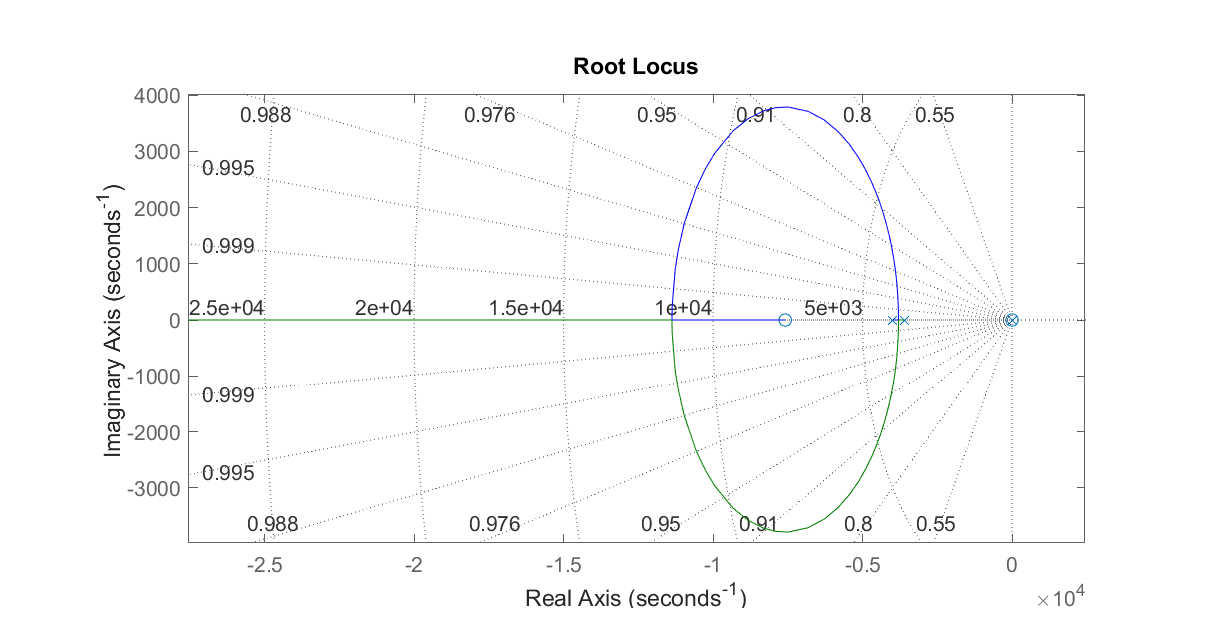
\includegraphics[width=1\textwidth]{Figures/rlocus_speed.eps}
	\caption[Root locus plot for the closed loop system.]{Root locus plot for the the closed loop system.}
	\label{fig:root_locus_speed}%chktex 24
\end{figure} % file "Thesis_Implementation.tex"
% \cleardoublepage{} 
\newpage

%%%%%%%%%%%%%%%%%%%%%%%%%%%%%%%%%%%%%%%%%%%%%%%%%%%%%%%%%%%%%%%%%%%%%%%%
%                                                                      %
%     File: Thesis_Results.tex                                         %
%     Tex Master: Thesis.tex                                           %
%                                                                      %
%     Author: Israel Sother                                            %
%     Last modified: 27 May 2024                                       %
%                                                                      %
%%%%%%%%%%%%%%%%%%%%%%%%%%%%%%%%%%%%%%%%%%%%%%%%%%%%%%%%%%%%%%%%%%%%%%%%

\chapter{Simulation and Experimental Results }
\label{chapter:results} %chktex 24
\minitoc% Creating a minitoc

%%%%%%%%%%%%%%%%%%%%%%%%%%%%%%%%%%%%%%%%%%%%%%%%%%%%%%%%%%%%%%%%%%%%%%%%
%                                                                      %
%     File: Simulation.tex		                                       %
%     Tex Master: Thesis.tex                                           %
%                                                                      %
%     Author: Israel Sother                                            %
%     Last modified: 27 May 2024                                       %
%                                                                      %
%%%%%%%%%%%%%%%%%%%%%%%%%%%%%%%%%%%%%%%%%%%%%%%%%%%%%%%%%%%%%%%%%%%%%%%%

\section{Simulation}
\label{section:simulation}%chktex 24
\vfill

To accelerate the development time, a model was developed in \textit{Simulink}, allowing for faster prototyping and direct comparison of the methods in a controlled environment. An adaptation of the \textit{Simscape Specialized Power Systems} block \textit{Permanent Magnet Synchronous Machine} was made to convert it to a delta-wound machine and to accept variable inductances as in \Cref{eq:motor_backward_euler_matrix}. 
This model was combined with six \glspl{mosfet} blocks in three legs to simulate the \gls{vsi}. To supply the \glspl{mosfet}, a model of the battery was made, where an ideal voltage source is connected through a series resistor to the DC link, where a capacitor stabilizes the voltage. In \Cref{fig:simulation_model} the resultant system is presented, where $S_1$, $S_2$, $S_3$, $S_4$, $S_5$, $S_6$, are the gate control signals that come from the control strategy.

\begin{figure}[!htb]
	\centering
	% \fbox{
		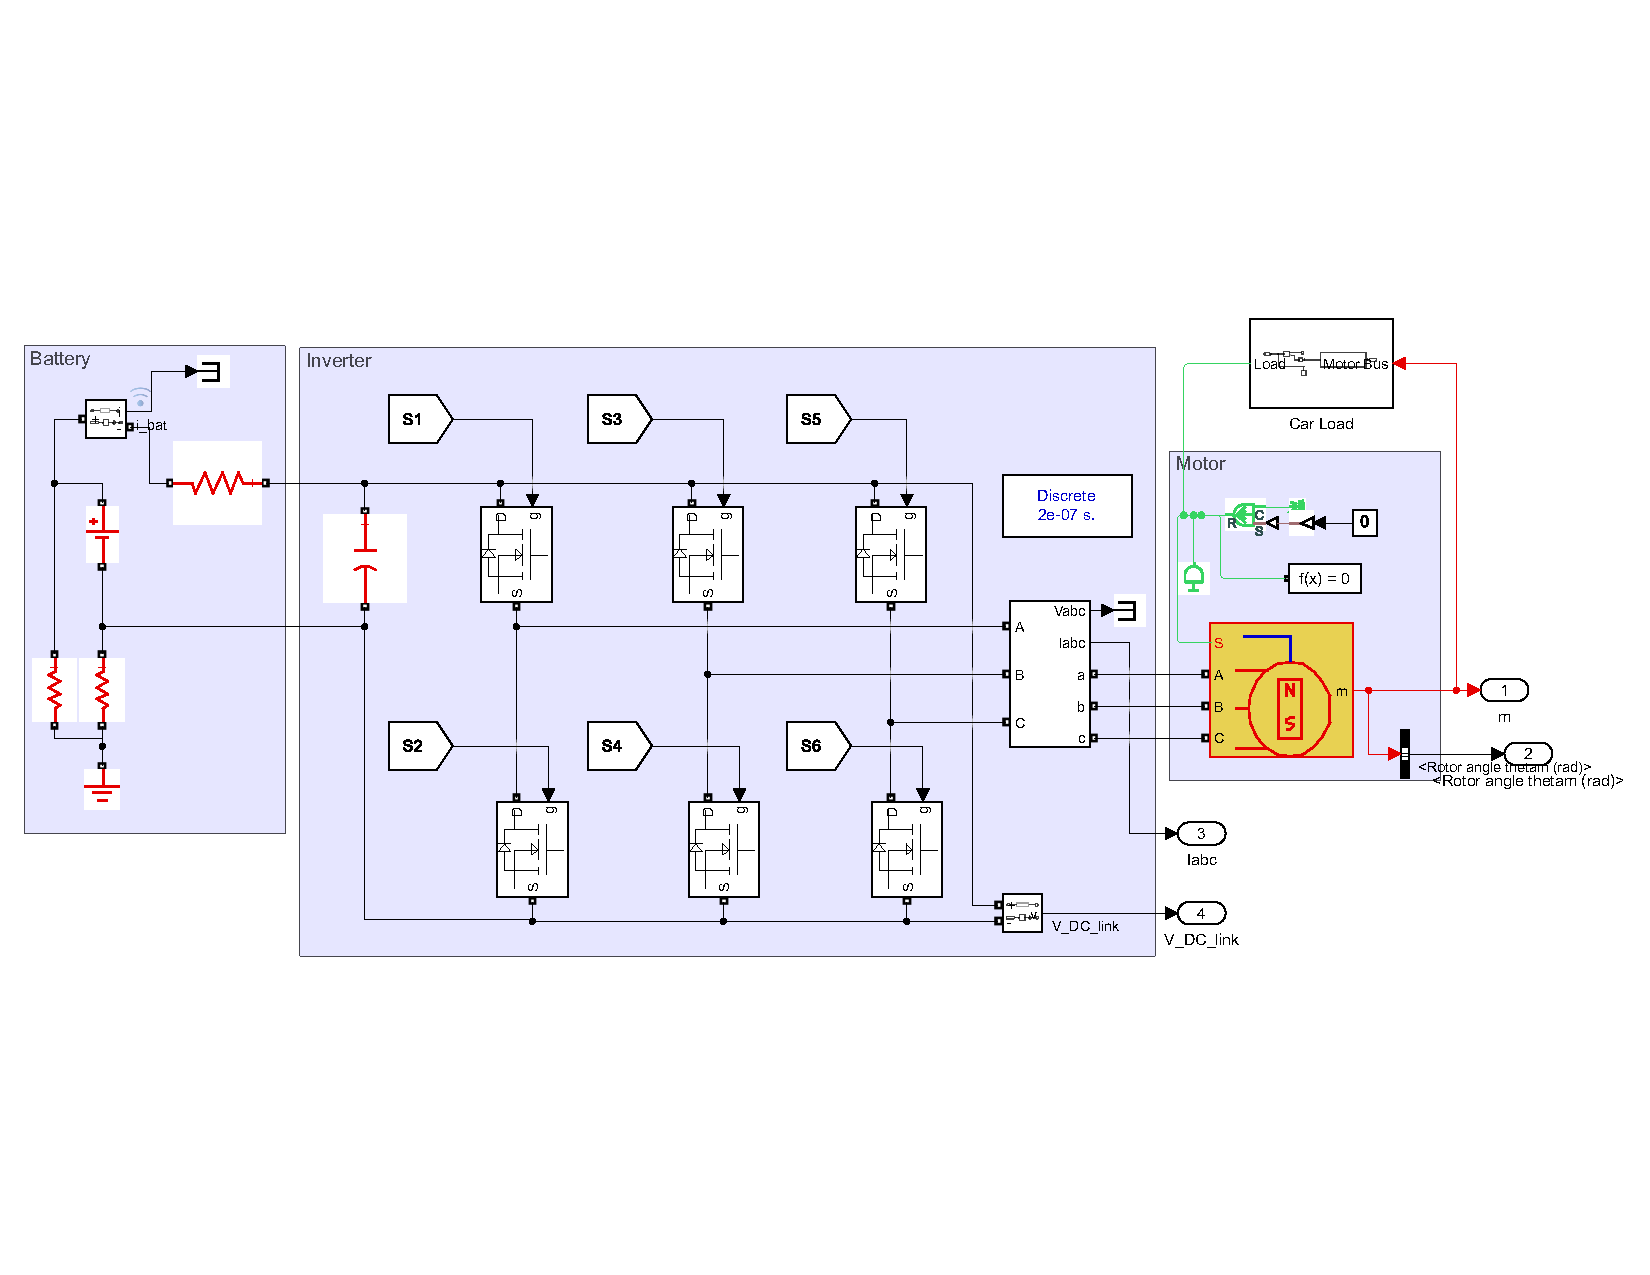
\includegraphics[clip, trim=0.3cm 5cm 0.5cm 5cm, width=1.00\textwidth]{Figures/motor_and_inverter_simulink1.pdf}
		% }
	\caption[Simulink Models, Motor and Inverter.]{Simulink Models, Motor and Inverter.}
	\label{fig:simulation_model} %chktex 24
\end{figure}

The parameterization of the \glspl{mosfet} used in the simulation is derived from the model used in~\cite{Costa:MSc}, the  Wolfspeed C2M0040120D. The motor model is the one derived on \Cref{section:PMSM model}, with the parameters from \Cref{section:motor_characterization}. The rotor position is based on Heidenhain ECI1118 properties as this is the encoder that the manufacturer uses. 
The DC link capacitor is set to $40\mu F$, while the battery series resistance is $0.03 \Omega$, both based on the existing hardware. The ground connections are $420k\Omega$ each, to simulate the isolation between high voltage and low voltage in the car, while the inertia and torque source blocks inside the motor area are to simulate the testbench environment, with the standard value of $0.0848 kg m^2$ to the inertia, and the torque source being controlled to maintain a constant speed. All those parameters are shown in \Cref{table:simulation_parameters} alongside the car parameters used in the load simulation on \Cref{section:acceleration}.

\begin{table}[h]
	\caption{Simulation Parameters}
	\label{table:simulation_parameters}%chktex 24
	\renewcommand{\arraystretch}{1.2} % more space between rows
	% \centering
	\begin{minipage}{0.49\textwidth}
		\centering
		\begin{tabular}{ll}
			\toprule
			\textbf{Simulation timestep} & $0.2\mu s$ \\\toprule
			\textbf{DC Link Capacitor} & $40\mu F$ \\\toprule
			\textbf{Battery Series Resistance} & $0.03 \Omega$ \\\toprule
			\textbf{Ground Connection} & $420k\Omega$ \\\toprule
			\textbf{Testbench Inertia} & $185 g cm^2$ \\\toprule
			\textbf{MOSFETs} & \begin{tabular}[c]{@{}l@{}}Wolfspeed \\ C2M0040120D\end{tabular} \\\toprule
			\textbf{Switching Frequency} & $50kHz$ \\\toprule
			\textbf{Encoder Resolution} & 18 bits \\\toprule
			\textbf{Encoder Frequency} & $12.5kHz$ \\\toprule
			\textbf{\begin{tabular}[c]{@{}l@{}}Current and Voltage \\ Sensor Resolution\end{tabular}} & 14 bits \\\toprule
			\textbf{\begin{tabular}[c]{@{}l@{}}Current and Voltage \\ Sensor Frequency\end{tabular}} & $50kHz$ \\\toprule
		\end{tabular}
	\end{minipage}
	% \hfill
	% \hspace{0.1cm}
	\begin{minipage}{0.49\textwidth}
		\centering
		\begin{tabular}{ll}
			\toprule
			\textbf{Car mass}                       & $230 kg$                      \\\toprule
			\textbf{Pilot mass}                     & $60 kg$                       \\\toprule
			\textbf{Tire radius}                    & $0.23 m$                      \\\toprule
			\textbf{\begin{tabular}[c]{@{}l@{}}Wheel assembly \\ moment of inertia\end{tabular}} & $0.2 kg m^2$ \\\toprule
			\textbf{Gear ratio}                     & $15.21$                       \\\toprule
			\textbf{Air density}                    & $1.2 kg/m^3$ \\\toprule
			\textbf{Reference car area}             & $1 m^2$      \\\toprule
			\textbf{Drag coefficient}               & $1.59$                        \\\toprule
			\textbf{Rolling resistance coefficient} & $0.09$                     \\\toprule
			\textbf{\begin{tabular}[c]{@{}l@{}}Speed Controller \\ proportional gain ($k_p$)\end{tabular}} & $0.035 Nm/rpm$ \\ \toprule
			\textbf{\begin{tabular}[c]{@{}l@{}}Speed Controller \\ integral gain ($k_i$)\end{tabular}}   & $10^{-9} Nm/rpm$ \\ \toprule
		\end{tabular}
	\end{minipage}
\end{table}

\subsection{Baseline Step}
With the model implemented on \textit{Simulink}, a baseline was made using the manufacturer control scheme, \gls{foc} with the standard $8kHz$ switching frequency, and compared with the proposed methods at $50kHz$. The difference in frequency is to account for the complete system, where the use of wide bandgap semiconductors allowed for a faster switching frequency. The baseline profile is a positive torque step with the machine fixed at the nominal speed of $12kRPM$. The rising time of each method is shown in \Cref{fig:rising_time_4_models}.
\begin{figure}[!htb]
	\centering
	\begin{subfigmatrix}{1}
		\subfigure[MPCs comparison. In orange the Finite set MPC, in yellow the finite set MPC with null vector, in green the continuous set implicit MPC, and in purple the proposed continuous set explicit MPC.]{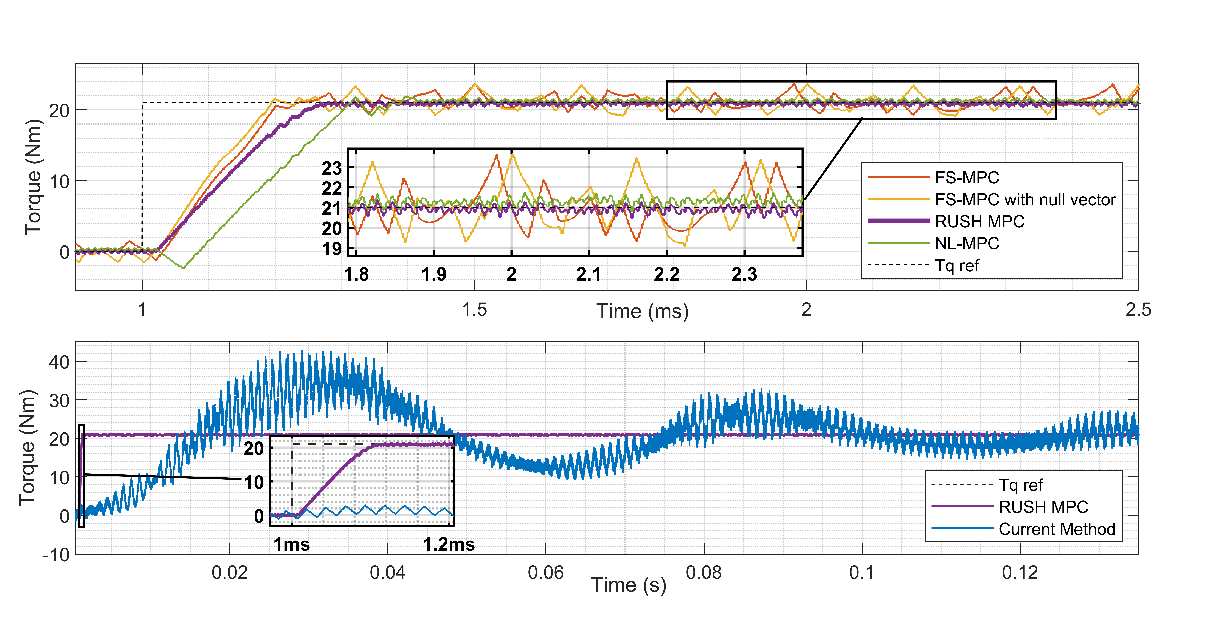
\includegraphics[clip, trim=0cm 4.8cm 0cm 0.75cm,width=1\textwidth]{Figures/Step_@12000RPM.eps}}
	\end{subfigmatrix}	
	\begin{subfigmatrix}{1}
		\subfigure[Proposed method (in purple) vs Currently used method (in blue).]{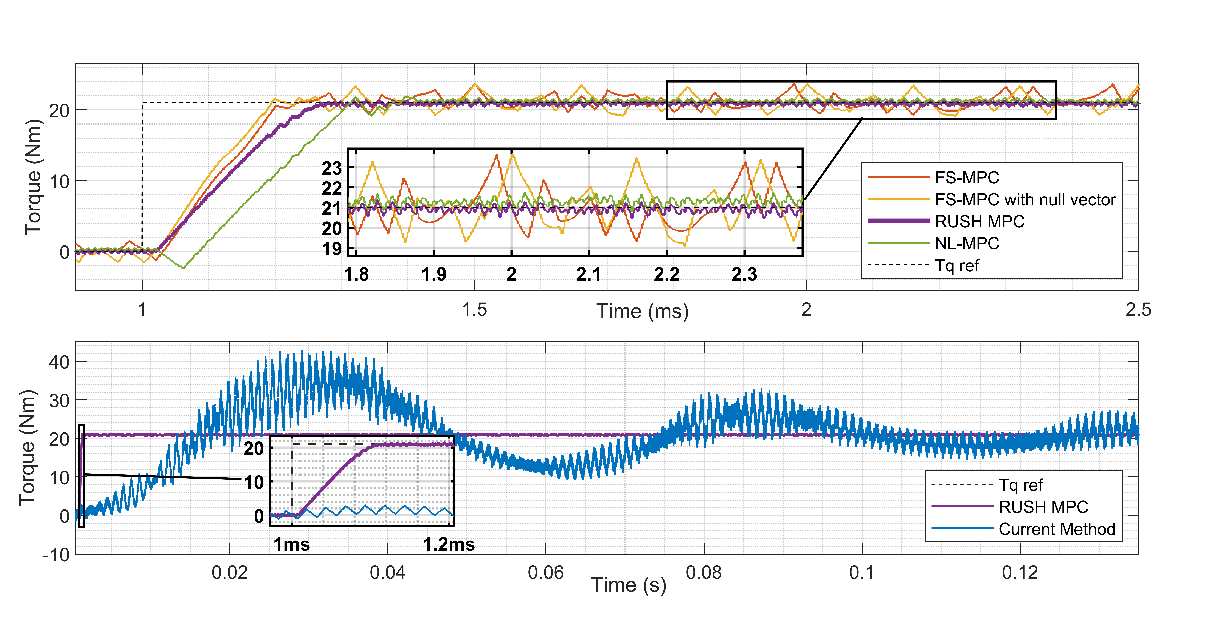
\includegraphics[clip, trim=0cm 0cm 0cm 5.5cm,width=1\textwidth]{Figures/Step_@12000RPM.eps}}
	\end{subfigmatrix}
	\caption[Control methods comparison in a torque step.]{Control methods comparison in a torque step.}
	\label{fig:rising_time_4_models} %chktex 24
\end{figure}

Note that the predictive controllers all perform similarly, having a good dynamic response, with an average rising time (0 to 100\%) of $200\mu s$, while the \gls{foc} method performed much slower, at approximately $180ms$. While the rising time in the \gls{foc} can be improved by better tunning the PID (these results are with the values recommended by the manufacturer), it would result in more pronounced overshoots and settling time, and would not reach the performance of a predictive controller, where the torque rising is only limited by the machine inductances, which shows the great dynamic performance of predictive controllers. It is important to also notice a small delay in the implicit \gls{nlmpc} response, this delay is due to the solver failing to converge. Although this may not always occur at each reference torque step, it was intentionally left on this graph to remind us of the possibility of this event. 

Divergence among the proposed methods becomes apparent during the analysis of steady-state conditions. The basic \gls{fsmpc} stands out with the highest torque and current ripple, significantly worse than the baseline, rendering it impractical. This ripple is due to the absence of a modulator, thus the chosen vector will stay applied for the full sampling time. Although an increase in switching frequency would improve the absolute performance of this method, in comparison it would never be as smooth as a modulated control, as it uses discrete vector options, while a simple \gls{svm} would switch multiple times in a single period. The increased switching reduces the ripple at the cost of lowered efficiency due to switching losses.

The addition of the null vector on the second method reduces the ripple at low angular speeds but still fails to do so when the machine accelerates, with curves very similar to the \gls{fsmpc}. The use of complete modulators can reduce this torque ripple problem, as the \gls{svm} allows for a third vector to be applied during the same time step, allowing the control to accurately point the voltage vector to the desired angle and amplitude, where the null vector only lets the controller change the amplitude of the existent active vectors.
\subsection{Current THD}

The distortion of currents was evaluated by setting the motor at a constant speed, waiting a few periods for it to reach a steady state and then calculating the average \gls{thd} of all line currents through 5 electrical periods. This was repeated in a grid pattern with some of the results shown in \Cref{table:thd_comparison}.

\begin{table}[h]
	\caption{Control Method Current THD comparison. THD is calculated until the Nyquist frequency, that is $250kHz$ and $40kHz$ for the controllers running at $50kHz$ and $8kHz$ respectively.}
	\label{table:thd_comparison}%chktex 24
	\renewcommand{\arraystretch}{1.2} % more space between rows
		\centering
		% \resizebox{1\textwidth}{!}{%
		\begin{tabular}{lrcccc}
			\textbf{} &
			  \multicolumn{1}{l}{\textbf{}} &
			  \textbf{1000 RPM} &
			  \textbf{7333 RPM} &
			  \textbf{13666 RPM} &
			  \textbf{20000 RPM} \\ \toprule
			 &
			  \textbf{1Nm} &
			  57.62\% &
			  43.44\% &
			  207.54\% &
			  29.62\% \\
			 &
			  \textbf{11Nm} &
			  3.22\% &
			  10.62\% &
			  12.14\% &
			  58.53\% \\
			\multirow{-3}{*}{\textbf{\begin{tabular}[c]{@{}l@{}}FOC \\ @8kHz\end{tabular}}} &
			  \textbf{20Nm} &
			  5.15\% &
			  6.50\% &
			  10.18\% &
			  37.08\% \\ \toprule
			 &
			  \textbf{1Nm} &
			  56.95\% &
			  11.08\% &
			  14.12\% &
			  4.71\% \\
			 &
			  \textbf{11Nm} &
			  2.18\% &
			  2.19\% &
			  1.93\% &
			  4.85\% \\
			\multirow{-3}{*}{\textbf{\begin{tabular}[c]{@{}l@{}}FOC \\ @50kHz\end{tabular}}} &
			  \textbf{20Nm} &
			  1.41\% &
			  1.41\% &
			  2.28\% &
			  3.86\% \\ \toprule
			 &
			  \textbf{1Nm} &
			  696.41\% &
			  566.94\% &
			  247.13\% &
			  72.31\% \\
			 &
			  \textbf{11Nm} &
			  39.42\% &
			  30.17\% &
			  28.04\% &
			  11.82\% \\
			\multirow{-3}{*}{\textbf{\begin{tabular}[c]{@{}l@{}}FS-MPC \\ @50kHz\end{tabular}}} &
			  \textbf{20Nm} &
			  22.10\% &
			  16.88\% &
			  8.52\% &
			  11.82\% \\ \toprule
			 &
			  \textbf{1Nm} &
			  30.67\% &
			  120.31\% &
			  159.20\% &
			  221.12\% \\
			 &
			  \textbf{11Nm} &
			  1.59\% &
			  10.65\% &
			  12.40\% &
			  11.51\% \\
			\multirow{-3}{*}{\textbf{\begin{tabular}[c]{@{}l@{}}FS-MPC \\ Null Vector \\ @50kHz\end{tabular}}} &
			  \textbf{20Nm} &
			  1.76\% &
			  6.43\% &
			  7.10\% &
			  8.54\% \\ \toprule
			 &
			  \textbf{1Nm} &
			  6.59\% &
			  9.98\% &
			  12.60\% &
			  14.50\% \\
			 &
			  \textbf{11Nm} &
			  0.81\% &
			  1.48\% &
			  1.89\% &
			  2.17\% \\
			\multirow{-3}{*}{\textbf{\begin{tabular}[c]{@{}l@{}}NL-MPC \\ @50kHz\end{tabular}}} &
			  \textbf{20Nm} &
			  0.81\% &
			  0.96\% &
			  1.18\% &
			  1.12\% \\ \bottomrule
			 &
			  \textbf{1Nm} &
			  7.20\% &
			  11.91\% &
			  16.82\% &
			  21.95\% \\
			 &
			  \textbf{11Nm} &
			  0.76\% &
			  1.47\% &
			  1.92\% &
			  2.16\% \\
			\multirow{-3}{*}{\textbf{\begin{tabular}[c]{@{}l@{}}RUSH MPC \\ @50kHz\end{tabular}}} &
			  \textbf{20Nm} &
			  0.81\% &
			  0.98\% &
			  1.19\% &
			  1.12\% \\ \toprule
			\end{tabular}
		% }
\end{table}

Table \ref{table:thd_comparison} exposes the advantage of continuous \gls{mpc} over the other alternatives, with distortions expressively smaller than the baseline and the finite set \glspl{mpc}, backing up the ripple analysis previously made. As expected the addition of a null vector reduced expressively the \gls{thd} in operation points of low modulation index, but made no difference when the modulation index increased. When comparing the methods that use \gls{svm}, the distortion is very similar when operated at the same frequency, meaning that the main factor is the modulation frequency, not the control algorithm.

Another advantage of the proposed methods is they actively use the direct axis current to generate torque throughout the full operation map of the motor,  not only in field weakening as the method currently implemented on the car. This is a result of the use of \gls{mtpa} references which improves efficiency, as it produces a reduction in the current vector modulus necessary to generate the same torque.
\subsection{Robustness}

To test the controller's robustness, a Monte Carlo analysis is proposed. A normal distribution is assigned to the motor parameters with a mean equal to the characterized value, and a standard deviation equal to 5\% of the mean. The step of \Cref{fig:rising_time_4_models} was simulated for 1000 samples with the modified parameters applied to the motor without updating the controller (\Cref{fig:montecarlo}).

\begin{figure}[!htb]
	\centering
	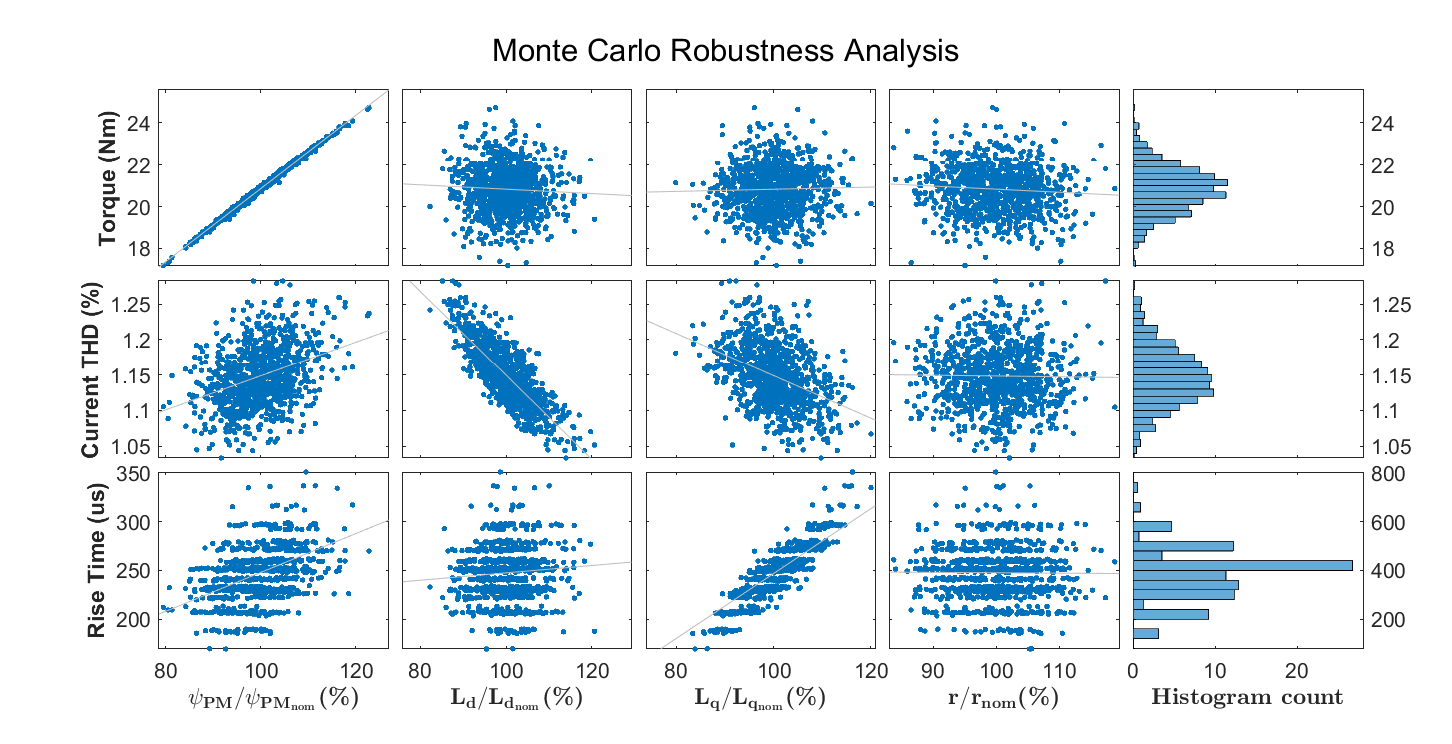
\includegraphics[width=1\textwidth]{Figures/MonteCarlo.eps}
	\caption[Monte Carlo Robustness Analysis.]{Monte Carlo Robustness Analysis. The motor parameters are shown in percentual change from the controller's expected value.}
	\label{fig:montecarlo} %chktex 24
\end{figure}

To evaluate the performance with degraded parameters three metrics were used, the steady-state mean torque, the steady-state current \gls{thd}, and the torque rising time. Based on these metrics the most influential parameter is the flux linkage, with a correlation of almost 100\% with the steady-state torque as shown in \Cref{fig:corr_plot}. This is explained by the type of motor used, where the inductances between the direct and quadrature axes are very similar, resulting in most of the torque derived from the permanent magnet's flux linkage. Note that this dependency is also present in the method currently used by the team, where the quadrature current reference is based on the machine torque constant ($k_t$). 
While relatively easy to characterize, the flux linkage is also the parameter most prone to change with the life of the motors, where the magnets can overheat or be demagnetized by a high direct axis current, thus a good approach is to develop a characterization routine that can be automatically executed whenever the user deems necessary.

\begin{figure}[!htb]
	\begin{subfigmatrix}{2}
		\subfigure[Steady State Torque]{\includegraphics[width=0.4\linewidth]{Figures/corr_tq.eps}\label{fig:corr_tq}}
		\subfigure[Current THD]{\includegraphics[width=0.4\linewidth]{Figures/corr_thd.eps}\label{fig:corr_thd}}
	\end{subfigmatrix}
	\begin{subfigmatrix}{1}
		\subfigure[Torque Rise Time]{\includegraphics[width=0.4\linewidth]{Figures/corr_risetime.eps}\label{fig:corr_risetime}}
	\end{subfigmatrix}
	\caption{Parameter correlation coefficient with performance metrics.}
	\label{fig:corr_plot}%chktex 24
\end{figure}

The quadrature inductance has a higher correlation with the torque rise time, as expected. Since almost all of the torque is derived from the permanent magnet's flux linkage the torque will rise as fast as the controller manages to create quadrature currents. While this correlation is not definitive proof, it reinforces the statement that the proposed controller dynamic response is limited by the machine inductances. The high flux linkage correlation with the rise time is due to the increase in steady-state torque since with higher flux the steady-state torque is higher and the rise is approximately linear, with an increase in steady-state torque the rise time also increases.

Regarding the current \gls{thd}, the parameter influences are well balanced, with the direct axis inductance being a little more correlated. When combining this with the small absolute variance of the \gls{thd}, it is clear that the control strategy is very robust against model mismatches, maintaining a low distortion even with the wrong parameters.

\subsection{Acceleration Event}
\label{section:acceleration}%chktex 24

The load profile defined in \Cref{section:03load_profile} was used to simulate a typical acceleration event. The car load parameters are as shown in \Cref{table:simulation_parameters}, and the torque reference was set to reach $21.3kW$ of delivered power (after inverter and motor efficiency losses). The power value was chosen assuming an $80\%$ powertrain efficiency and the previous approximation of one-third of the car load on the rear motors. As shown in \Cref{fig:acceleration_comparison}, the \gls{rush} improved the time from $3.943s$ to $3.883s$ ($1.6\%$), reaching also a higher top speed than the currently implemented control method and presenting a lower torque ripple. While the $0.06s$ seems like a small gain, comparing with the results from \gls{fsg} 2023 it would put \gls{fst} three positions higher in the event ranking. If the proposed control method is combined with the efficiency improvement from the use of new inverter hardware, the time is further reduced, to $3.759s$ ($4.7\%$), translating to a 6 position gain in the event ranking.

\begin{figure}[!htb]
	\centering
	\begin{subfigmatrix}{2}
		\subfigure[Torque profile in the acceleration event using the currently implemented FOC.]{\includegraphics[clip,trim = 1cm 0 1.55cm 0,width=0.49\linewidth]{Figures/acc_empc.eps}\label{fig:acc_foc}}
		\subfigure[Torque profile in the acceleration event using the proposed EMPC]{\includegraphics[clip,trim = 1cm 0 1.55cm 0,width=0.49\linewidth]{Figures/acc_foc.eps}\label{fig:acc_empc}}
	\end{subfigmatrix}
	\begin{subfigmatrix}{2}
		\subfigure[Motor speed profile in the acceleration event. The blue line is the currently implemented FOC while the orange line is the proposed EMPC.]{\includegraphics[width=0.49\linewidth]{Figures/acc_rpm.eps}\label{fig:acc_rpm}}
		\subfigure[Distance traveled in the acceleration event. The blue line is the currently implemented FOC while the orange line is the proposed EMPC.]{\includegraphics[width=0.475\linewidth]{Figures/acc_dist.eps}\label{fig:acc_dist}}
	\end{subfigmatrix}
	\caption[Control methods comparison on an Acceleration event.]{Control methods comparison on an Acceleration event.}
	\label{fig:acceleration_comparison} %chktex 24
\end{figure}
%%%%%%%%%%%%%%%%%%%%%%%%%%%%%%%%%%%%%%%%%%%%%%%%%%%%%%%%%%%%%%%%%%%%%%%%
%                                                                      %
%     File: Experimental.tex	                                       %
%     Tex Master: Thesis.tex                                           %
%                                                                      %
%     Author: Israel Sother                                            %
%     Last modified: 27 May 2024                                       %
%                                                                      %
%%%%%%%%%%%%%%%%%%%%%%%%%%%%%%%%%%%%%%%%%%%%%%%%%%%%%%%%%%%%%%%%%%%%%%%%
\section{Experimental Results}
\label{section:experimental}%chktex 24
\vfill

To validate the simulated results, some tests were made on a test bench. The \gls{rush} was implemented using Xilinx Model Composer inside Simulink, compared with the simulation implementation and then generated for the \gls{fpga} present in a Digilent Zybo Z7-20. The hardware used was comprised of the inverter developed on~\cite{Costa:MSc}, coupled with a current measuring board, developed for this thesis to increase noise immunity. This pairing was supplied with a power supply by Elektro-Automatik (EA-PSI 8360-15 DT) capable of up to 1.5kWh, and the characterized AMK motor was set in a test bench with a Sensor Technology torque transducer (RWT441-EC-PG) and another AMK motor as load. The complete setup is shown in \Cref{fig:testbench_steup}.

The inverter used in the experimental setup was a limiting factor due to the chosen semiconductors not being able to handle the maximum motor current. This limitation was explained in~\cite{Costa:MSc}, where it was mentioned that the intended \gls{mosfet} was not available, thus an alternative semiconductor had to be used. The evolution of the \gls{sic} semiconductors since the previous design was also noticeable, going from a second \gls{sic} \gls{mosfet} generation to a fourth, improving reliability and efficiency. Those limitations, combined with the advances in the \gls{sic} semiconductors industry exposed the need for a new hardware version. Even though this work focuses on the controller development, not the hardware, a new inverter design was made, covering the limitations of the current one. This new inverter design was not ready for the experimental tests, but a brief chapter on the design process is included in \Cref{chapter:appendix_inverter}.

\begin{figure}[!htb]
	\centering
	\includegraphics[width=.8\textwidth]{Figures/testbench_setup.jpg}
	\caption[Testbench setup.]{Testbench setup.}
	\label{fig:testbench_steup} %chktex 24
\end{figure}

First, a simple constant torque test was made to evaluate if the model was correctly calculating the generated torque. \Cref{fig:constant_tq} presents the torque estimated based on the motor parameters and the current measurements with the value measured with the ST transducer output. The current measurement from the developed measurement board had some outliers from \gls{emi}, so the currents and torque in this section were filtered using a moving median (8 samples) and if the sample is further than 2 \gls{mad}, then it is considered an outlier, thus it is replaced by the average of the closest 2 points.

\begin{figure}[!htb]
	\centering
	\includegraphics[width=0.8\linewidth]{Figures/constantTq.eps}
	\caption[Torque estimation vs Measured. In the bottom the percentual error between the measured and estimated torques is shown.]{Torque estimation vs Measured. At the bottom, the percentual error between the measured and estimated torques is shown.}
	\label{fig:constant_tq} %chktex 24
\end{figure}

The estimated torque is constantly smaller than the measured torque, with a difference of 0.5Nm. This difference is due to the motor parameters not being perfectly matched with the real motor, and the current measurements not being perfect. The difference between the estimated and measured torque is small enough to consider the model valid for the next tests.

With the torque estimation validated, the next step was to verify the currents on a steady state test, ideally, this would be done with nominal torque, but due to a limited maximum inverter current the motor was commanded to keep a constant torque of $7Nm$. To create a load, another motor was connected to the shaft and the motor phases were short-circuited, creating a load torque that changes with the speed, this resulted in the speed stabilizing at $269RPM$. The current was measured with the developed measuring board and with an oscilloscope probe (ELDITEST CP6550), while the torque was estimated by the control algorithm and compared with the simulation results. The simulation results were obtained by running the same model used for the controller implementation, with the same parameters and inputs. The results are presented in \Cref{fig:steady_state_curr}.
\begin{figure}[!htb]
	\begin{subfigmatrix}{2}
		\subfigure[Measurement Board and Simulation measurements. The plot on top present values from the measurement board, while the bottom plot is from the simulation.]{\includegraphics[width=0.47\linewidth]{Figures/const_curr_7NM.eps}\label{fig:steady_state_curr_sim_meas}}
		\subfigure[Oscilloscope measurements. Channel 1 (in yellow) represents the line A current, while channel 2 (in blue) is the line B current]{\includegraphics[width=0.52\linewidth]{Figures/const_curr_osc_7nm-01.eps}\label{fig:steady_state_curr_osc}}
	\end{subfigmatrix}
	\caption{Line currents measured at steady state. Torque reference at $7Nm$ and rotor speed stable at $169RPMs$.}
	\label{fig:steady_state_curr} %chktex 24
\end{figure}

 The oscilloscope measurement was made with a probe that has a sensitivity of $20mV/A$. The results show that the current measured by the developed board is identical to the one from the oscilloscope probe, proving the system's accuracy. When comparing the measured currents with the simulation results, although they have the same form and amplitude, it is clear that the simulated curve is cleaner. This is backed by the \gls{thd} comparison, where the measured current has a \gls{thd} of $2.44\%$ and the simulated current has a \gls{thd} of $0.47\%$, both of them calculated to the 50th harmonic. This difference is due to inaccuracies in the measurements and parametrization. 
% While noisier, the measured current is still a great improvement over the previous control method, where the simulated current had a \gls{thd} of $1.65\%$.

Then a torque step response was applied with the motor at a standstill and with the same load as the constant current test. Once again it would be a good approach to use the nominal values but the inverter was a limitation so a reference of $7Nm$ was used. The currents presented in \Cref{fig:tq_step_fig} show an almost instantaneous dynamic response, transitioning to the specified amplitude without noticeable distortions. The oscilloscope currents are also very similar to the ones measured by the developed board, with the same form and amplitude. The simulation results are very similar to the measured ones, with the same form and amplitude, but the simulation is cleaner.  The difference between the measured and simulated currents is small enough to consider the model valid.
\begin{figure}[!htb]
	\begin{subfigmatrix}{2}
		\subfigure[Measurement Board and Simulation measurements. The plot on top presents values from the measurement board, while the bottom plot is from the simulation.]{\includegraphics[width=0.47\linewidth]{Figures/tq_step_curr.eps}\label{fig:tq_step_curr}}
		\subfigure[Oscilloscope measurements. Channel 1 (in yellow) represents the line A current, while channel 2 (in blue) is the line B current]{\includegraphics[width=0.52\linewidth]{Figures/tq_step_osc-01.eps}\label{fig:tq_step_osc}}
	\end{subfigmatrix}
	\caption{Line Current measurements with a reference torque step from $0$ to $7Nm$ at $0.02s$.}
	\label{fig:tq_step_fig} %chktex 24
\end{figure}



\Cref{fig:tq_step_response_time} shows the torque dynamic response to the step. The reduced sampling time creates significant uncertainty in the measurement, but it is possible to state that the torque rise time is less than 200 microseconds, which is a great improvement when compared with the current control method. The simulation results have a greater sampling rate showing that the rise time is smaller than 100 microseconds. An improved sampling frequency would allow for a better comparison between the simulation and experimental results.

\begin{figure}[!htb]
	\centering
	\includegraphics[width=0.55\linewidth]{Figures/Tq_step.eps}
	\caption[Torque reference following with a step from $0$ to $7Nm$.]{Torque reference following with a step from $0$ to $7Nm$. The upper plot presents the experimental data, while the bottom plot is from the simulation}
	\label{fig:tq_step_response_time} %chktex 24
\end{figure}

To compare the performance of the proposed method, a torque step was also applied to the current solution of the inverter and control strategy. The results presented in \Cref{fig:torque_step_comparison_FOC_MPC} show that as expected, the current solution is much slower than the proposed method, with a rising time of $30ms$ and a delay of $10ms$. When compared with the simulated values in \Cref{fig:rising_time_4_models} a difference can be seen in the overshoot value of the current method, which is not present in the experimental results.  That is due to the gains used on the PI current controller, which are not as aggressive as the ones used in the simulation. This also resulted in a slower rising time, as in the simulation it reached the $10Nm$ mark in half the time as the experimental results.

\begin{figure}[!htb]
	\centering
	\includegraphics[width=0.7\linewidth]{Figures/Car_Tq_step.eps}
	\caption{Comparison of torque step response between the proposed method and the currently implemented method.}
	\label{fig:torque_step_comparison_FOC_MPC}%chktex 24
\end{figure}

The torque step response was repeated for several reference torque values, from $1$ to $10Nm$, to evaluate the tracking capabilities of the controller. The results presented in \Cref{fig:tq_step_response_multiple} show that the \gls{rush} is capable of tracking the reference torque independently of its magnitude. The rising time stayed constant throughout the steps, being smaller than the sampling time of $157\mu s$. It can also be seen that there is not a pronounced overshoot. 

\begin{figure}[!htb]
	\centering
	\begin{subfigmatrix}{3}
		\subfigure[$1Nm$]{\includegraphics[width=0.31\linewidth]{Figures/torque_step_1Nm_tq.eps}\label{fig:torque_step_1Nm}}
		\subfigure[$3Nm$]{\includegraphics[width=0.31\linewidth]{Figures/torque_step_3Nm_tq.eps}\label{fig:torque_step_3Nm}}
		\subfigure[$5Nm$]{\includegraphics[width=0.31\linewidth]{Figures/torque_step_5Nm_tq.eps}\label{fig:torque_step_5Nm}}
	\end{subfigmatrix}
	\begin{subfigmatrix}{3}
		\subfigure[$6Nm$]{\includegraphics[width=0.31\linewidth]{Figures/torque_step_6Nm_tq.eps}\label{fig:torque_step_6Nm}}
		\subfigure[$7Nm$]{\includegraphics[width=0.31\linewidth]{Figures/torque_step_7Nm_tq.eps}\label{fig:torque_step_7Nm}}
		\subfigure[$8Nm$]{\includegraphics[width=0.31\linewidth]{Figures/torque_step_8Nm_tq.eps}\label{fig:torque_step_8Nm}}
	\end{subfigmatrix}
	\subfigure[$10Nm$]{\includegraphics[width=0.31\linewidth]{Figures/torque_step_10Nm_tq.eps}\label{fig:torque_step_10Nm}}
	\caption{Torque step response for different reference torque values.}
	\label{fig:tq_step_response_multiple}
\end{figure}


To test the speed controller, an RPM step was applied with the motor at standstill and without load. In \Cref{fig:speed_step_fig} the rotor speed and the torque are presented. The speed controller was saturated to $\pm 5Nm$ to avoid overcurrents as the power supply was not able to constantly supply high currents. A small overshoot can be seen in the speed response, this is due to the exponential average filter that was implemented on the RPM measure. The filter reduced the bandwidth of the signal and when combined with high gains in the PI it produced some oscillations which can be improved with a less aggressive filter and a better-tuned PI controller. The \gls{rush} has great tracking capabilities, as shown by the torque graph, with the estimated torque overlaying the reference torque. The error between the torque reference and the estimated torque is shown in \Cref{fig:rpm_step_tq_error}, showing an average error of $0.05Nm$ and a peak error of $0.9Nm$.


\begin{figure}[!htb]
	\centering
	\subfigure[RPM reference and measured values.]{\includegraphics[width=0.8\linewidth]{Figures/rpm_step_rpm.eps}\label{fig:rpm_step_rpm}}
	\\
	\subfigure[Torque reference and measured values. The torque reference is derived from the speed controller but saturated to $\pm 5Nm$.]{\includegraphics[width=0.8\linewidth]{Figures/rpm_step_tq.eps}\label{fig:rpm_step_tq}}
	\\
	\subfigure[Torque reference tracking error. ]{\includegraphics[width=0.8\linewidth]{Figures/rpm_step_tq_error.eps}\label{fig:rpm_step_tq_error}}
	\caption{RPM step from standstill to 2500RPMs.}
	\label{fig:speed_step_fig} %chktex 24
\end{figure}

A torque profile to simulate the driver's input was also tested and is presented in \Cref{fig:pedal_profile}. The controller fails to output the reference torque around $0.1s$ due to the power supply not being able to provide enough current, thus it switched from constant voltage to constant current output, reducing the available voltage to the inverter. Aside from this, the controller was able to follow the torque reference with a small error, averaging $0.04Nm$ and peaking at $1.6Nm$ if the period of the power supply shortage is discarded.
%  A small dependency on the speed can be seen in the torque tracking error, with the error slightly increasing with the rotor velocity. This is seen in the torque ripple increasing, due to the increased back \gls{emf} that requires the controller to increase the modulation index to keep the current amplitude, resulting in saturation

\begin{figure}[!htb]
	\centering
	\subfigure[Line Currents.]{\includegraphics[width=0.85\linewidth]{Figures/pedal_profile_curr.eps}\label{fig:pedal_profile_curr}}
	\\
	\subfigure[Rotor speed.]{\includegraphics[width=0.85\linewidth]{Figures/pedal_profile_rpm.eps}\label{fig:pedal_profile_rpm}}
	\\
	\subfigure[Torque reference and measured values. The torque reference is derived from the speed controller but saturated to $\pm 5Nm$.]{\includegraphics[width=0.85\linewidth]{Figures/pedal_profile_tq.eps}\label{fig:pedal_profile_tq}}
	\\
	\subfigure[Torque reference tracking error. ]{\includegraphics[width=0.85\linewidth]{Figures/pedal_profile_tq_error.eps}\label{fig:pedal_profile_error}}
	\caption{Pedal torque profile.}
	\label{fig:pedal_profile} %chktex 24
\end{figure}
\newpage

%\input{Thesis_new_file} % add new .tex files for new chapters
%\cleardoublepage{} 

%\input{Thesis_new_file} % add new .tex files for new chapters
%\cleardoublepage{} 

%\input{Thesis_new_file} % add new .tex files for new chapters
%\cleardoublepage{} 

% \input{04Thesis_Simulation.tex} % file "Thesis_Results.tex"
% \cleardoublepage{} 
% \newpage

%%%%%%%%%%%%%%%%%%%%%%%%%%%%%%%%%%%%%%%%%%%%%%%%%%%%%%%%%%%%%%%%%%%%%%%%
%                                                                      %
%     File: Thesis_Conclusions.tex                                     %
%     Tex Master: Thesis.tex                                           %
%                                                                      %
%     Author: Israel Sother                                            %
%     Last modified: 27 May 2024                                       %
%                                                                      %
%%%%%%%%%%%%%%%%%%%%%%%%%%%%%%%%%%%%%%%%%%%%%%%%%%%%%%%%%%%%%%%%%%%%%%%%

\chapter{Conclusions}
\label{chapter:conclusions}
% \minitoc% Creating a minitoc

The work developed in this thesis aimed to fill the identified gap in the process of a powertrain developed fully in-house for the \gls{fst} that is the control strategy for the motors. This necessity led to a study of control strategies and motor models that was performed with an emphasis on improving the dynamic response of the motor torque and the system efficiency.

To achieve those goals, the motor was characterized by performing several measurements and tests. This not only provided a plant model to simulate the control algorithms but also provided the Formula Student team of Instituto Superior Técnico with valuable information about their motor characteristics and performance.

 With the motor parametrized, it was possible to set up a simulation environment and some control strategies were implemented in it. This allowed a comparison between the different strategies and the selection of the most suitable for the application. The selected strategy was the \acrfull{rush} due to its fast response, low current ripple, and computational efficiency. 

The proposed control was then implemented in an \gls{fpga} and the hardware necessary to test the control in a test bench was developed. The motors and inverter were then assembled on a test bench to perform experimental tests. Although the testbench hardware was later verified to be a limiting factor, the experimental results were very promising.

The simulation and experimental results were compared and analyzed showing a close match between them. The torque estimation was also validated and the control strategy was able to control the motor torque with a dynamic response orders of magnitude smaller than the current solution and with a very low torque ripple. The system efficiency was also improved due to the reduction in current \gls{thd}.

While not exhaustive the developed system continued to build on the great work of the previous thesis and the team's work, creating a solid platform from which the team can continue the work and implement it on the next prototypes. The work done in this thesis was a major step towards the team's goal of developing a fully in-house powertrain.
% ----------------------------------------------------------------------
\section{Achievements}
\label{section:achievements}

The major achievement of the present work was the development of a control strategy capable of greatly increasing the dynamic response of the motor while also improving its efficiency. This work showed that by changing the control strategy there are performance gains to be achieved without hardware changes, only by using a control strategy that is tailored to the motor characteristics. The ability to control the currently used motor without any hardware modifications on the motor enables the team to develop its own inverter and control strategy without changing the motor, unlocking major advances in powertrain efficiency, performance, and density. Additionally, it provided some valuable information about the motor characteristics and performance that can be used in future work and at competition design events.

Summing up the achievements of this thesis, the following points can be highlighted:
\begin{itemize}
    \item The currently used motor is characterized and a simulation environment was created;
    \item Several \gls{mpc} strategies were compared with the current \gls{foc} solution leading to the selection of the \gls{rush};
    \item The proposed control strategy was implemented in an \gls{fpga};
    \item The necessary hardware for a test bench setup was developed and tested to a high level of accuracy;
    \item Simulation data was validated with experimental results comparison;
    \item Motor characterization validated by comparing the torque estimation with a commercial transducer;
    \item System efficiency improved by the reduction of the current \gls{thd};
    \item The torque response was improved by orders of magnitude compared to the current solution.
    \item A new inverter was designed to overcome the limitations of the current one.
\end{itemize}


% ----------------------------------------------------------------------
\section{Future Work}
\label{section:future}

One of the major setbacks of this work was the test bench hardware, which was later verified to be a limiting factor. The used setup was not able to properly align the motor shafts and the transducer, leading to excentricity-induced vibrations. Those vibrations not only caused some torque oscillations in the experimental results but also limited the tested maximum speed. The test bench hardware should be redesigned to allow for a proper alignment of the motor shafts and the transducer, allowing for higher speeds and more accurate results.

The inverter used was also deemed a limitation, as it was developed to a maximum current of $90A$, limiting the maximum torque that could be applied to the motor. A revision of the inverter was developed, but time constraints impeded it to be tested. The new inverter should be tested to verify if the limitations of the current inverter are overcome and to verify if it meets the efficiency and performance requirements of the team. Some design aspects of the inverter should also be revised, such as the thermal design of the components, and the DC link capacitance, which could be reduced to save space and weight. The voltage measurement circuit should also be revised to include filters and improve the \gls{emi} immunity of the system. 

Regarding the motor characterization, the inverter limitations did not allow for a full current range characterization of the inductances, which could be performed in the future. The current reference maps should also be updated with the maps generated using the characterization inductances, to replace the ones that used the manufacturer's data. 

A proper study of the tradeoff between the reduction of the current \gls{thd} by increasing the switching frequency and the losses in the inverter and motor derived from such increase should be performed. An optimal point should be found to maximize the efficiency of the system.

A known drawback of the chosen strategy is the dependence on a good model of the system. A calibration routine should be developed to allow for the controller to automatically adjust the model parameters to the real system. Another alternative is the development of a real-time parameter identification algorithm to adjust the model parameters in real-time, but this would require the current references to be solved in real-time, similar to the work done in~\cite{Jung:Online_MTPA_Ferrari:2013}.

The current implementation uses the rotor speed to estimate the current position of the rotor in between encoder readings, which is a known limitation of the system. A better approach would be to use the \gls{mpc} predictions to estimate the rotor position, which would also benefit from a load torque observer, to improve the velocity and position predictions.

The proposed speed controller although capable of controlling the motor speed, could be improved, as it was not the focus of this work. It could be incorporated into the \gls{mpc} controller and account for the load torque estimation to preemptively adjust the torque reference to allow for a more robust control.

Another known limitation is the encoder sampling rate, which is very reduced when compared to the control frequency. That, combined with the elevated level of complexity of the encoder protocol and its scarce documentation, suggests that the encoder should be replaced by a more modern and faster sensor.

Lastly, the current implementation of the \gls{fpga} uses almost all the available resources, which limits the implementation of more complex algorithms. It also is currently controlling only one motor, but by pipelining the control, it could control two motors, limited by the number of available GPIOs in the Zybo board. One solution could be to switch the control algorithm from floating point to fixed point, which would require fewer resources and would allow for more complex algorithms to be implemented. Another solution would be to use a more powerful \gls{fpga}, which would also enable the control of the four motors in only one \gls{fpga}, reducing the cost and volume of the system. % file "Thesis_Conclusions.tex"
% \cleardoublepage{} 
\newpage

% ----------------------------------------------------------------------
%  Bibliography
% ----------------------------------------------------------------------

% Add entry in the table of contents as chapter
\phantomsection{}
\addcontentsline{toc}{chapter}{\bibname}

% Include all references in .bib file, even non-cited ones...
%\nocite{*} % this should be used carefully because it is not correct!

% Produces the bibliography section when processed by BibTeX
%
% Bibliography style
% > entries ordered alphabetically
%\bibliographystyle{plain}
% > unsorted with entries appearing in the order in which the citations appear.
% \bibliographystyle{unsrt}
% > entries ordered alphabetically, with first names and names of journals and months abbreviated
%\bibliographystyle{abbrv}
% > entries ordered alphabetically, with reference markers based on authors' initials and publication year
%\bibliographystyle{alpha}
%
% Replacement bibliography styles provided by 'natbib' package
% (plainnat.bst, abbrvnat.bst, unsrtnat.bst )
% > entries ordered alphabetically
%\bibliographystyle{plainnat}
% > unsorted with entries appearing in the order in which the citations appear.
%\bibliographystyle{unsrtnat}
% > entries ordered alphabetically, with first names and names of journals and months abbreviated
%\bibliographystyle{abbrvnat} % <<<<< SELECT IF USING REFERENCES BY AUTHOR/YEAR
% > entries ordered alphabetically, with reference markers based on authors' initials and publication year
%\bibliographystyle{alpha}
%
% Custom bibliography style adapted from 'natbib' package
%   (based on http://tex.stackexchange.com/questions/5053/is-it-possible-to-get-unsrt-abbrv-bibliography)
%   (unsrtnat.bst + abbrvnat.bst -> abbrvunsrtnat.bst)
%   (original files copied from:
%   http://tug.ctan.org/macros/latex/contrib/natbib/abbrvnat.bst
%   http://tug.ctan.org/macros/latex/contrib/natbib/unsrtnat.bst
% > unsorted with entries appearing in the order in which the citations appear, with first names and names of journals and months abbreviated.
\bibliographystyle{Packages/abbrvunsrtnat} % <<<<< SELECT IF USING REFERENCES BY NUMBER (CITATION ORDER)

\setlength{\bibsep}{0.0pt}
% External bibliography database file in the BibTeX format
\bibliography{Thesis_bib_DB} % file "Thesis_bib_DB.bib"

% \cleardoublepage{} 
\newpage

% ----------------------------------------------------------------------
%  Appendix (optional)
%
%  CAUTION: 1) the main document (up to the conclusions) shall not exceed 80 pages
%           2) the document shall not exceed a total of 100 pages (per IST regulations)
% ----------------------------------------------------------------------
\appendix

% add page number prefix according to apendix chapter (optional)
%\renewcommand{\thepage}{\thechapter.\arabic{page}}

% re-set arabic numbering (A.1,A.2,...) (optional, use only if chapter prefix is added)
% \setcounter{page}{1}

%%%%%%%%%%%%%%%%%%%%%%%%%%%%%%%%%%%%%%%%%%%%%%%%%%%%%%%%%%%%%%%%%%%%%%%%
%                                                                      %
%     File: Thesis_Appendix_A.tex                                      %
%     Tex Master: Thesis.tex                                           %
%                                                                      %
%     Author: Israel Sother                                            %
%     Last modified: 27 May 2024                                       %
%                                                                      %
%%%%%%%%%%%%%%%%%%%%%%%%%%%%%%%%%%%%%%%%%%%%%%%%%%%%%%%%%%%%%%%%%%%%%%%%
\chapter{Amplitude invariant dq0 PMSM model}
\label{chapter:appendixdq0_amplitude}

Starting with \Cref{eq:flx_voltage_balance} and replacing the currents and flux for the ones presented in \Cref{eq:variables_dq0} results in \Cref{eq:flx_voltage_balance_abc_to_dq}.

\begin{equation}
	\begin{aligned}
		\mathbf{u_{abc}}
		=
		\mathbf{R_{abc}}
		\mathbf{T}^*_{(\theta_e)} \mathbf{i_{dq0}}
		+
		\frac{d\left(\mathbf{T}^*_{(\theta_e)} \pmb{\psi_{dq0}}\right)}{dt}
		\\
		=
		\mathbf{R_{abc}}
		\mathbf{T}^*_{(\theta_e)} \mathbf{i_{dq0}}
		+\dot{\theta}_e\frac{d\mathbf{T}^*_{(\theta_e)}}{d\theta_e}\pmb{\psi_{dq0}}
		+\mathbf{T}^*_{(\theta_e)}\frac{d \pmb{\psi_{dq0}}}{dt}
	\end{aligned}
	\label{eq:flx_voltage_balance_abc_to_dq}
\end{equation}

Replacing $\dot{\theta}_e$ with $\omega_e$, and multiplying ${\mathbf{T}^*_{(\theta_e)}}^{-1}$ to the left yields \Cref{eq:flx_voltage_balance_abc_to_dq_transform,eq:flx_voltage_balance_abc_to_dq_transform1}.
\begin{equation}
	\begin{aligned}
		\mathbf{u_{dq0}}
		=
		\mathbf{R_{dq0}}\mathbf{i_{dq0}}
		+{\mathbf{T}^*_{(\theta_e)}}^{-1}\omega_e\frac{d\mathbf{T}^*_{(\theta_e)}}{d\theta_e}\pmb{\psi_{dq0}}
		+{\mathbf{T}^*_{(\theta_e)}}^{-1}\mathbf{T}^*_{(\theta_e)}\frac{d \pmb{\psi_{dq0}}}{dt}
	\end{aligned}
	\label{eq:flx_voltage_balance_abc_to_dq_transform}
\end{equation}
\begin{equation}
	\begin{aligned}
		\mathbf{u_{dq0}}
		=
		\mathbf{R_{dq0}}\mathbf{i_{dq0}}
		+\omega_e{\mathbf{T}^*_{(\theta_e)}}^{-1}\frac{d\mathbf{T}^*_{(\theta_e)}}{d\theta_e}\pmb{\psi_{dq0}}
		+\frac{d \pmb{\psi_{dq0}}}{dt}
	\end{aligned}
	\label{eq:flx_voltage_balance_abc_to_dq_transform1}
\end{equation}
Lastly, calculate the derivative of the transformation as in \Cref{eq:transformation_derivative_ampl}, resulting in \Cref{eq:transformation_derivative_ampl_result}.
\begin{equation}
	{\mathbf{T}^*_{(\theta_e)}}^{-1}\frac{d\mathbf{T}^*_{(\theta_e)}}{d\theta_e} = 	\frac{2}{3}
	\begin{bmatrix}
		\cos{\left(\theta_e\right)}		&	\cos{\left(\theta_e-\frac{2\pi}{3}\right)}		&	\cos{\left(\theta_e-\frac{4\pi}{3}\right)}	\\
		-\sin{\left(\theta_e\right)} 	&	-\sin{\left(\theta_e-\frac{2\pi}{3}\right)}		&	-\sin{\left(\theta_e-\frac{4\pi}{3}\right)}	\\
		\frac{1}{2}						&					\frac{1}{2}						&				 \frac{1}{2}					 \\
	\end{bmatrix}
	\begin{bmatrix}
		-\sin{\left(\theta_e\right)}                & -\cos{\left(\theta_e\right)}                & 0 \\
		-\sin{\left(\theta_e-\frac{2\pi}{3}\right)} & -\cos{\left(\theta_e-\frac{2\pi}{3}\right)} & 0 \\
		-\sin{\left(\theta_e-\frac{4\pi}{3}\right)} & -\cos{\left(\theta_e-\frac{4\pi}{3}\right)} & 0 \\
	\end{bmatrix}
	\label{eq:transformation_derivative_ampl}
\end{equation}
\begin{equation}
	{\mathbf{T}^*_{(\theta_e)}}^{-1}\frac{d\mathbf{T}^*_{(\theta_e)}}{d\theta_e} =
	\begin{bmatrix}
		0 & -1 & 0 \\
		1 & 0  & 0 \\
		0 & 0  & 0 \\
	\end{bmatrix}
	\label{eq:transformation_derivative_ampl_result}
\end{equation}
Thus, the \gls{pmsm} model in the dq0 frame using amplitude invariant transformation is presented in \Cref{eq:flx_voltage_balance_dq0_amplitude}. This result is the same as \Cref{eq:flx_voltage_balance_dq0}with the currents, voltages, and fluxes scaled by a factor of $\sqrt{\frac{3}{2}}$ in the direct and quadrature axis, but in the zero axis some results may vary.
\begin{equation}
	\mathbf{u_{dq0}}
	=
	\mathbf{R_{dq0}}\mathbf{i_{dq0}}
	+\omega_e	\begin{bmatrix}
		0 & -1 & 0 \\
		1 & 0  & 0 \\
		0 & 0  & 0 \\
	\end{bmatrix}
	\pmb{\psi_{dq0}}
	+\frac{d \pmb{\psi_{dq0}}}{dt}
	\label{eq:flx_voltage_balance_dq0_amplitude}
\end{equation} % file "Thesis_Appendix_A.tex"
% \newpage
% \cleardoublepage{} 

% re-set arabic numbering (B.1,B.2,...) (optional, use only if chapter prefix is added)
% \setcounter{page}{1}

%%%%%%%%%%%%%%%%%%%%%%%%%%%%%%%%%%%%%%%%%%%%%%%%%%%%%%%%%%%%%%%%%%%%%%%%
%                                                                      %
%     File: Thesis_Appendix_B.tex                                      %
%     Tex Master: Thesis.tex                                           %
%                                                                      %
%     Author: Israel Sother                                            %
%     Last modified: 27 May 2024                                       %
%                                                                      %
%%%%%%%%%%%%%%%%%%%%%%%%%%%%%%%%%%%%%%%%%%%%%%%%%%%%%%%%%%%%%%%%%%%%%%%%

\chapter{Technical Datasheets}
\label{chapter:appendixDatasheets} %chktex 24

The datasheets for the current inverter and motor used in the project are presented in this appendix. The inverter datasheet is an excerpt from the original document with the main characteristics, while the motor datasheet is the full document. More information about the kit is available at the manufacturer's website\footnote{\url{https://www.amk-motion.com/amk-dokucd/dokucd/en/DokuCD_HTML5_en.htm\#projekt/doku-cd_html5/topics/amk_automotive.htm}}.

% It is possible to add PDF files to the document, such as technical sheets of some equipment used in the work.

% ----------------------------------------------------------------------
% See more options to include PDF files in
% http://mirror.unl.edu/ctan/macros/latex/contrib/pdfpages/pdfpages.pdf
% \includepdf[pages={1-2},nup=1x2,landscape=true]{Figures/SolarCell_Sunpower_C60.pdf}
\def\excerpt{\section{AMK Motor Datasheet}\label{section:AMK_Motor_datasheet}}
\includepdf[pages={1},nup=1x1,landscape=true,scale=0.9,pagecommand={\excerpt}]{./Appendix/motor_data_sheet_a2370dd_dd5.pdf}
\includepdf[pages={2},nup=1x1,landscape=true,scale=0.9,pagecommand={}]{./Appendix/motor_data_sheet_a2370dd_dd5.pdf}

% \section{AMK Inverter Datasheet}
% \label{section:AMK_Inverter_datasheet} %chktex 24
\includepdf[pages={16},nup=1x1,landscape=false,scale=0.8,pagecommand=\section{AMK Inverter Datasheet}
\label{section:AMK_Inverter_datasheet}]{./Appendix/pdk_205481_kw26-s5-fse-4q_en_.pdf}
\includepdf[pages={17},nup=1x1,landscape=false,scale=0.9,pagecommand={}]{./Appendix/pdk_205481_kw26-s5-fse-4q_en_.pdf}
 % file "Thesis_Appendix_B.tex"
\newpage

%%%%%%%%%%%%%%%%%%%%%%%%%%%%%%%%%%%%%%%%%%%%%%%%%%%%%%%%%%%%%%%%%%%%%%%%
%                                                                      %
%     File: Thesis_Appendix_C.tex                                      %
%     Tex Master: Thesis.tex                                           %
%                                                                      %
%     Author: Israel Sother                                            %
%     Last modified: 27 May 2024                                       %
%                                                                      %
%%%%%%%%%%%%%%%%%%%%%%%%%%%%%%%%%%%%%%%%%%%%%%%%%%%%%%%%%%%%%%%%%%%%%%%%
\chapter{Current Reference using characterized inductances}
\label{chapter:appendix_current_reference}

As explained in \Cref{section:inductance_curves_current_reference}, the used current references on the experimental results were not calculated using the inductance values obtained from the motor characterization. This section presents the current references calculated using the characterized curves.

\begin{figure}[!htb]
	\begin{subfigmatrix}{2}
		\subfigure[Minimum Voltage]{\includegraphics[width=0.49\linewidth]{Figures/Motor_map@420V_charact}\label{fig:mtpa_Constrained_420_charac}}
		\subfigure[Nominal Voltage]{\includegraphics[width=0.49\linewidth]{Figures/Motor_map@532V_charact}\label{fig:mtpa_Constrained_540_charac}}
	\end{subfigmatrix}
	\begin{subfigmatrix}{1}
		\subfigure[Maximum Voltage]{\includegraphics[width=0.49\linewidth]{Figures/Motor_map@600V_charact}\label{fig:mtpa_Constrained_588_charac}}
	\end{subfigmatrix}
	\caption{Constrained Maximum Torque per Ampere curve at minimum, nominal, and maximum voltages. Reference currents are shown for 0, 13000 and 2000 RPMs.}
	\label{fig:mtpa_constrained_new}%chktex 24
\end{figure}

An important distinction to make is that the curves in \Cref{fig:mtpa_constrained_new} present an inversion in torque signal depending on the direct axis current. This is due to the reluctance torque reaching and surpassing the torque generated by the permanent magnets. This phenomenon is due to the saturation effect, which reduces the quadrature axis inductance, while the direct axis inductance increases. % file "Thesis_Appendix_C.tex"
\newpage

%%%%%%%%%%%%%%%%%%%%%%%%%%%%%%%%%%%%%%%%%%%%%%%%%%%%%%%%%%%%%%%%%%%%%%%%
%                                                                      %
%     File: Thesis_Appendix_D.tex                                      %
%     Tex Master: Thesis.tex                                           %
%                                                                      %
%     Author: Israel Sother                                            %
%     Last modified: 27 May 2024                                       %
%                                                                      %
%%%%%%%%%%%%%%%%%%%%%%%%%%%%%%%%%%%%%%%%%%%%%%%%%%%%%%%%%%%%%%%%%%%%%%%%
\chapter{Inverter Design}
\label{chapter:appendix_inverter}

The new inverter design was intended to solve the current and voltage measurement issues that were present in the previous design, while also increasing the maximum current supported by the inverter. It was mainly designed using the same process as~\cite{Costa:MSc}. The design process started with the selection of the semiconductor devices based on an efficiency analysis, followed by the design of the gate drivers and the current and voltage measurement circuits. As this version of the inverter was intended to be used in the next prototypes, a special focus was given to reducing further the size of the inverter, while also making it more modular to allow for easier maintenance and replacement of components.

\section{Efficiency Equation Formulation}

To ease the process of choosing the semiconductor efficiency analysis approach was used. This was performed with the efficiency formulation for a three-phase inverter from~\cite{Costa:SiC_MOSFET_losses:2023}, as it represents well the system developed. In~\cite{Costa:SiC_MOSFET_losses:2023} the power loss is assumed to be majorly composed by the semiconductor losses, as the inverter does not have magnetic components. This assumption is based on~\cite{Song:SiC_MOSFET_losses:2019}, where it is stated that the power losses of SiC \gls{mosfet} chips in the power module account for more than 93.4\% of the total power losses of the power inverter.

The power losses of the \gls{mosfet} chips can be divided into conduction losses and switching losses defined as in~\cite{Costa:SiC_MOSFET_losses:2023}. The conduction losses are given by \Cref{eq:conduction_losses}.

\begin{equation}
	\frac{P_{ON}}{P_o} = \frac{R_{DS_{on}}}{R_0} (1+THD^2)
	\label{eq:conduction_losses}
\end{equation}

Where $P_{ON}$ is the conduction losses, $P_o$ is the output power, $R_{DS_{on}}$ is the on-state resistance of the \gls{mosfet}, $R_0$ is the load equivalent resistance and $THD$ is the total harmonic distortion of the output current.

The switching losses are presented in \Cref{eq:switching_losses}.

\begin{equation}
	\frac{P_{SW}}{P_o} = \left( \frac{\sqrt(3)}{2\pi m_p F_p}\frac{t_{on}+t_{off}}{T}+\frac{3 C_t Z_0}{m_p^2 F_p T} \right)(3-m_p)
	\label{eq:switching_losses}
\end{equation}

Where $P_{SW}$ is the switching losses,$Z_0$ is the load equivalent impedance defined as $Z_0 = \frac{R_0}{F_p}$ with $F_p$ being the load power factor, $t_{on}$ and $t_{off}$ are the turn-on and turn-off times of the \gls{mosfet}, $T$ is the switching period, $C_t$ is the total parasitic capacitance defined as $C_t = C_{oss} + C_d$ with $C_{oss}$ being the \gls{mosfet} output parasitic capacitance, and $C_d$ the external diode parasitic capacitance. The modulation index $m_p$ used in this formulation is different from the one used on the control scheme, and it is defined as $\sqrt{6} V_{ORMS}/V_{DC}$ where $V_{ORMS}$ is the line to neutral output RMS voltage.

The complete efficiency formulation is presented in \Cref{eq:efficiency}.

\begin{equation}
	\eta = \frac{1}{1 + \frac{P_{ON}}{P_o} + \frac{P_{SW}}{P_o}} = \frac{1}{1 + \frac{R_{DS_{on}}}{F_p Z_0} (1+THD^2) + \left( \frac{\sqrt{3}}{2\pi m_p F_p}\frac{t_{on}+t_{off}}{T}+\frac{3 C_t R_0}{m_p^2 F_p^2 T} \right)(3-m_p)}
	\label{eq:efficiency}
\end{equation}

\subsection{Motor and Controller parameters}
With the efficiency equation defined, the next step was to define the load parameters, in this case, the motor operation points. As the power factor of the motor changes with the motor speed and torque, a map of the power factor was used. This map is derived from manufacturer data and is presented in \Cref{fig:motor_power_factor}. As the manufacturer only provided the power factor for positive torque, the power factor for negative torque was assumed to be the same as the power factor for positive torque. While this is not accurate, it is a good approximation for the efficiency analysis.
\begin{figure}[H]
	\centering
	\begin{subfigmatrix}{2}
		\subfigure[Motor power factor.]{\includegraphics[width=0.45\linewidth]{Figures/motor_power_factor.eps}\label{fig:motor_power_factor}}
		\subfigure[Current THD.]{\includegraphics[width=0.45\linewidth]{Figures/THD_map.eps}\label{fig:THD_map}}
	\end{subfigmatrix}
	\caption{Motor power factor and current THD maps as a function of the motor speed and torque.}
	\label{fig:motor_power_factor_THD_map}
\end{figure}

The current \gls{thd} was calculated using the simulation environment presented in \Cref{section:simulation}. The motor was kept in a steady state for each of the operation points, and the current \gls{thd} was calculated. The results are presented in \Cref{fig:THD_map}.

\section{Operation Points}
As the load parameters are not constant a competition data-driven approach was taken to evaluate which module is better suited for the application. The logs from the 2023 competitions were used to create a 2-D histogram with the motor speed and torque usual operation points. \Cref{fig:motor_operation_points} presents the histogram of the operation points for each motor in the 2023 \gls{fsg} Endurance Event as an example.

\begin{figure}[H]
	\centering
	\includegraphics[trim=1cm 0.3cm 1.6cm 1cm, clip, width=0.8\textwidth]{Figures/Endurance_FSG_4wd.eps}
	\caption{Motor operation points for the 2023 Germany Endurance Event. The color represents the number of points in each bin on a logarithmic scale.}
	\label{fig:motor_operation_points}
\end{figure}

To generalize the design, each of the motor's operation points was combined, resulting in a single histogram with the operation points of all the motors. An example of the combined histogram is presented in \Cref{fig:motor_operation_points_combined}.

\begin{figure}[H]
	\centering
	\includegraphics[width=0.8\textwidth]{Figures/Endurance_FSG_combined.eps}
	\caption{Combined motor operation points for the 2023 Germany Endurance Event. The color represents the number of points in each bin on a logarithmic scale.}
	\label{fig:motor_operation_points_combined}
\end{figure}

With the operation points defined, the efficiency of the inverter was averaged using the operation points histogram as weights. This allowed a direct comparison of the average efficiency of each semiconductor in a representative competition environment. The results for the chosen module are presented in \Cref{fig:eff_graphs}.

\section{Diode Selection}
The antiparallel diode is used with two main functions, the first is to protect the \glspl{mosfet} from the reverse voltage generated by the motor inductance in case a fault occurs and the control shuts down the inverter while the motor is still spinning. Although in this case, the \gls{mosfet} body diode would allow the current to flow, it usually has a smaller forward current rating and a high forward voltage drop, thus in a failure mode it would heat the module and possibly damage it. The second reason is related to efficiency, as it allows the current that would flow through the \gls{mosfet} body diode to flow through the external diode, which has a smaller forward voltage drop, thus reducing the conduction losses in the dead time period.
To select the proper diode to parallel with the \glspl{mosfet}, the principal factors are the diode must support at least double the DC Link voltage in reverse voltage, and the peak current of the diode must be at least the peak current of the motor. The continuous current rating is not a concern here because in normal operation as soon as the \gls{mosfet} is turned on the diode will not conduct any current, as the \gls{mosfet} resistance produces a voltage drop smaller than the forward voltage of the diode. Ideally, the diode would be dimensioned to endure the peak current for the longest fault mode, but timing constraints prevented this study from being made, so it was dimensioned by the normal operation conditions of the motor datasheet~\cite{amk:DD5-14-10-POW}. The diode should also have a small parasitic capacitance to reduce the increase in the switching losses, and a low forward voltage drop to reduce the conduction losses in the dead time period.

\Cref{tab:diode_list} presents the list of possible diodes for the new inverter design compared with the one used on the current design.
\begin{table}[H]
	\centering
	\caption{List of possible diodes for the new inverter design compared to the solution used on the current design.}
	\label{tab:diode_list}
	\resizebox{\textwidth}{!}{%
	\begin{tabular}{ccccccccc}
		\toprule
		\textbf{Manufacturer} & \textbf{Model}    & \textbf{$\mathbf{V_{RRM}(V)}$} & \textbf{$\mathbf{V_f(V)}$} & \textbf{$\mathbf{I_f(A)}$} & \textbf{$\mathbf{I_{fsm}(A)}$} & \textbf{$\mathbf{C(pF)}$} & \textbf{$\mathbf{T_{MAX}(\degree C)}$} & \textbf{Price (\texteuro)} \\ \midrule
		ST			& STBR3012-Y        & 1200	& 0.95	& 30	& 300	& 15	& 175	& 2.62  	\\ 
		Littelfuse	& LSIC2SD120D15     & 1200	& 1.5	& 44	& 120	& 76	& 175	& 10.5  	\\ 
		Microchip	& MSC050SDA120B     & 1200	& 1.5	& 109	& 290	& 214	& 175	& 16.6  	\\ 
		GeneSiC		& GD60MPS17H        & 1700	& 1.5	& 122	& 600	& 252	& 175	& 42.85  	\\
		Vishay		& VS-E5TH3012S2L-M3 & 1200	& 1.9	& 30	& 240	& 17	& 175	& 2.76  	\\ \midrule
		Cree		& C4D10120E         & 1200	& 1.5	& 33	& 75	& 41.5	& 175	& 11.53  	\\ \bottomrule
	\end{tabular}%
}
\end{table}

Due to its reduced cost and good performance, the ST STBR3012-Y was chosen for the new inverter design. While this is not a \gls{sic} diode, it still fulfills the requirements for the application and presents the best performance on paper.

\section{MOSFET Module Selection}


To increase the inverter density and improve the thermal performance the semiconductors were limited to half-bridge modules, as they allow for a more compact design and easy integration, while also reducing the number of components needed. The use of the half-bridge configuration was also motivated by the modularity provided, as this simplifies the design to one inverter leg that can be replicated to compose the complete inverter. This modularity also allows for easier maintenance and replacement of components, at the cost of the reduced number of available semiconductors in the market.

As the battery voltage currently used is $600V$, the semiconductors needed to have a voltage rating of at least $1200V$. The maximum motor current is approximately $150A$, with a nominal current of $45A_{RMS}$, setting the minimum drain current rating of the \glspl{mosfet} to $45A$. The other parameters can be reasonably selected to maximize the efficiency of the inverter. Based on these initial requirements a list of possible \glspl{mosfet} was created and shown in \Cref{tab:mosfet_list}. Note that the $1700V$ semiconductors are significantly more expensive than the $1200V$ semiconductors, thus they are not considered for the final design.  The Microchip modules include Schottky diodes, while the other modules do not include the diodes, thus in the efficiency calculations the capacitance of the chosen diode was summed to the other modules to allow for a fair comparison.

% Please add the following required packages to your document preamble:
% \usepackage{graphicx}
\begin{table}[]
	\centering
	\caption{List of possible \gls{mosfet} modules for the new inverter design compared to the discrete solution used on the current design.}
	\label{tab:mosfet_list}
	\resizebox{\textwidth}{!}{%
		\begin{tabular}{ccccccccccccc}
			\toprule
			\textbf{Manufacturer} & \textbf{Model}             & \textbf{$\mathbf{V_{DSS} (V)}$} & \textbf{$\mathbf{R_{DS_{on}}(m\Omega)}$} & \textbf{$\mathbf{I_d(A)}$} & \textbf{$\mathbf{T_{max} \degree C}$} & \textbf{$\mathbf{C_{OSS}(pF)}$} & \textbf{$\mathbf{t_{on}(ns)}$} & \textbf{$\mathbf{t_{off}(ns)}$} & \textbf{Price (\texteuro)} \\ \midrule
			Infineon      & FF4MR12W2M1HP\_B11         & 1200    & 4       & 200     & 175     & 840      & 44      & 16      & 260.85   \\ 
			Infineon      & FF6MR12W2M1H\_B11          & 1200    & 5.4     & 150     & 175     & 630      & 39      & 15      & 194.88   \\ 
			Infineon      & FF08MR12W1MA1\_B11A        & 1200    & 7.33    & 150     & 150     & 700      & 35      & 38      & 268.99   \\ 
			Infineon      & FF8MR12W1M1H\_B11          & 1200    & 8.1     & 100     & 175     & 420      & 70      & 20      & 165.21   \\ 
			Infineon      & FF11MR12W2M1HP\_B11        & 1200    & 10.8    & 100     & 150     & 315      & 41.1    & 21.2    & 125.12   \\ 
			Microchip     & MSCSM170AM11CT3AG          & 1700    & 8.8     & 240     & 175     & 600      & 17      & 19      & 499.29   \\ 
			Microchip     & MSCSM170AM15CT3AG          & 1700    & 11.7    & 181     & 175     & 450      & 17      & 19      & 425.52   \\ 
			Microchip     & MSCSM120AM11CT3AG          & 1200    & 10.4    & 254     & 175     & 810      & 30      & 25      & 360.10   \\ 
			Microchip     & MSCSM120AM16CT1AG          & 1200    & 16      & 173     & 175     & 540      & 30      & 25      & 206.89   \\ 
			Semikron      & SK150MB120CR03TE2          & 1200    & 8       & 188     & 175     & 520      & 17      & 29      &          \\ 
			Vincotech     & 10-EZ122PA016ME-LJ67F68T   & 1200    & 17      & 83      & 175     & 258      & 6.72    & 21.48   &          \\ 
			Vincotech     & 10-EY122PA008ME01-LU38F06T & 1200    & 9.11    & 184     & 175     & 516      & 40      & 16.92   &          \\ \midrule
			Wolfspeed     & C2M0040120D                & 1200    & 44      & 55      & 150     & 171      & 61      & 13      & 45.94    \\ \bottomrule
		\end{tabular}%
	}
\end{table}

For each semiconductor in the list, an efficiency map was created using the efficiency formulation presented in \Cref{eq:efficiency}, and the operation points histogram presented in \Cref{fig:motor_operation_points_combined} was used to compute the average efficiency throughout the last \gls{fsg} Endurance event. The average results are presented in \Cref{tab:efficiency_comparison}.

\begin{table}[]
	\centering
	\caption{Efficiency comparison of the possible \glspl{mosfet} modules for the new inverter design.}
	\label{tab:efficiency_comparison}
	\resizebox{\textwidth}{!}{%
	\begin{tabular}{cccccc}
		\toprule		
		\textbf{Manufacturer} & \textbf{Model}             & \begin{tabular}[c]{@{}c@{}}\textbf{Conduction} \\ \textbf{Loss (W)}\end{tabular} &  \begin{tabular}[c]{@{}c@{}}\textbf{Switching} \\ \textbf{Loss (W)}\end{tabular}& \textbf{Efficiency (\%)} & \textbf{Price (\texteuro)} \\ \midrule
		Microchip             & MSCSM120AM16CT1AG          & 70.80         & 15.53  & 98.76      & 206.89         \\
		Vincotech             & 10-EZ122PA016ME-LJ67F68T   & 75.22         & 7.94   & 98.80      &                \\
		Infineon              & FF11MR12W2M1HP\_B11        & 47.78         & 15.66  & 99.08      & 125.12         \\
		Microchip             & MSCSM120AM11CT3AG          & 46.02         & 17.38  & 99.08      & 360.10         \\
		Microchip             & MSCSM170AM15CT3AG          & 51.77         & 10.83  & 99.09      & 425.52         \\
		Infineon              & FF8MR12W1M1H\_B11          & 35.84         & 22.34  & 99.16      & 165.21         \\
		Vincotech             & 10-EY122PA008ME01-LU38F06T & 40.31         & 15.88  & 99.19      &                \\
		Infineon              & FF08MR12W1MA1\_B11A        & 32.43         & 20.60  & 99.23      & 268.99         \\
		Microchip             & MSCSM170AM11CT3AG          & 38.94         & 11.85  & 99.26      & 499.29         \\
		Semikron              & SK150MB120CR03TE2          & 35.40         & 13.56  & 99.29      &                \\
		Infineon              & FF6MR12W2M1H\_B11          & 23.89         & 16.03  & 99.42      & 194.88         \\
		Infineon              & FF4MR12W2M1HP\_B11         & 17.70         & 18.76  & 99.47      & 260.85         \\ \midrule
		Wolfspeed             & C2M0040120D                & 194.69        & 17.19  & 97.00      & 45             \\ \bottomrule
	\end{tabular}
	}
\end{table}

Although it does not have the highest efficiency, the Infineon FF8MR12W1M1H\_B11~\cite{Infineon:Module_Datasheet:2023} was chosen as it has one of the smallest footprints, while having good efficiency and a reasonable price.  It also brings significant performance gains when compared to the discrete option used on the current inverter design that averaged at $97\%$ efficiency, and even more when compared with the inverter currently used on the vehicle, which averages at only $86\%$. One interesting factor to note here is the dominance of the conduction losses over the switching losses, indicating an increase in switching frequency could be beneficial to the efficiency of the inverter as it would reduce the current \gls{thd} and thus the conduction losses. The resulting inverter efficiency is presented in \Cref{fig:efficiency}.

% \begin{figure}[H]
% 	\centering
% 	\includegraphics[width=1\textwidth]{Figures/Infineon-FF8MR12W1M1H_B11_eff.eps}
% 	\caption{Ratio of Conduction and Switching losses against output power, and overall inverter efficiency using the Infineon FF8MR12W1M1H\_B11 module.}
% 	\label{fig:efficiency_inverter}
% \end{figure}

\pgfplotsset{
	contour/label node code/.code={%
		\node at (axis direction cs: 3200,0){$ $\pgfmathprintnumber{#1}$\%$};%
	}%
}
\begin{figure}[H]
	\centering
	\begin{subfigmatrix}{2}
		\subfigure[Conduction Loss Ratio.]{
			\begin{tikzpicture}
				\begin{axis}[
					height=7cm,
					width=0.45\linewidth,
					view={0}{90},
					mesh/ordering=x varies,
					mesh/cols=49,
					mesh/rows=60,
					xtick={4000,8000,12000,16000,20000},
					ymin=-21,
					ymax=21,
					xmin=700,
					xmax=20000,
					point meta min=-5, 
					point meta max=5,
					xlabel={RPM},
					ylabel={Torque (Nm)},
					shader=interp]
					\addplot3[samples=100, contour gnuplot={levels = {5,2,1,0.6,0.3,0.05},draw color=black,contour label style={every node/.append style={text=black}}},contour/draw color={black},contour/label distance=110pt] table[skip first n=2,x=x, y=y, z=z] {Figures/subplot_1.dat};
				\end{axis}
			\end{tikzpicture}
			\label{fig:cond_loss_ratio}
		}
		\subfigure[Switching Loss Ratio.]{
			\pgfplotsset{
				contour/label node code/.code={%
					\node at (axis direction cs: 0,0){$ $\pgfmathprintnumber{#1}$\%$};%
				}%
			}
			\begin{tikzpicture}
				\begin{axis}[
					height=7cm,
					width=0.45\linewidth,
					view={0}{90},
					mesh/ordering=x varies,
					mesh/cols=43,
					mesh/rows=60,
					xtick={4000,8000,12000,16000,20000},
					ymin=-21,
					ymax=21,
					xmin=700,
					xmax=20000,
					point meta min=-5, 
					point meta max=5,
					xlabel={RPM},
					ylabel={Torque (Nm)},
					shader=interp]
					\addplot3[samples=100, contour gnuplot={levels = {1.5,0.6,0.3,0.15,0.05},draw color=black,contour label style={every node/.append style={text=black}}},contour/draw color={black},contour/label distance=120pt] table[skip first n=2,x=x, y=y, z=z] {Figures/subplot_2.dat};
				\end{axis}
			\end{tikzpicture}
			\label{fig:sw_loss_ratio}
		}
	\end{subfigmatrix}
	\begin{subfigmatrix}{2}
		\subfigure[Total Loss Ratio.]{
			\begin{tikzpicture}
				\begin{axis}[
					height=7cm,
					width=0.45\linewidth,
					view={0}{90},
					mesh/ordering=x varies,
					mesh/cols=45,
					mesh/rows=60,
					xtick={4000,8000,12000,16000,20000},
					ymin=-21,
					ymax=21,
					xmin=700,
					xmax=20000,
					point meta min=-5, 
					point meta max=5,
					xlabel={RPM},
					ylabel={Torque (Nm)},
					shader=interp]
					\addplot3[samples=100, contour gnuplot={levels = {5,3,1.5,1,0.5,0.25,0.05},draw color=black,contour label style={every node/.append style={text=black}}},contour/draw color={black},contour/label distance=140pt] table[skip first n=2,x=x, y=y, z=z] {Figures/subplot_3.dat};
				\end{axis}
			\end{tikzpicture}
			\label{fig:total_loss_ratio}
		}
		\subfigure[Efficiency.]{
			\begin{tikzpicture}
				\begin{axis}[
					height=7cm,
					width=0.45\linewidth,
					view={0}{90},
					mesh/ordering=x varies,
					mesh/cols=45,
					mesh/rows=60,
					xtick={4000,8000,12000,16000,20000},
					ymin=-21,
					ymax=21,
					xmin=700,
					xmax=20000,
					point meta min=-5, 
					point meta max=5,
					xlabel={RPM},
					ylabel={Torque (Nm)},
					shader=interp]
					\addplot3[samples=100, contour gnuplot={levels = {95,97.5,98.5,99,99.25,99.5,99.7},draw color=black,contour label style={every node/.append style={text=black}}},contour/draw color={black},contour/label distance=165pt] table[skip first n=2,x=x, y=y, z=z] {Figures/subplot_4.dat};
				\end{axis}
			\end{tikzpicture}
			\label{fig:efficiency}
		}
	\end{subfigmatrix}
	\caption{New inverter losses analysis.}
	\label{fig:eff_graphs}
\end{figure}


\section{Gate Driver Design}

\acrshort{asr}
\acrfull{mpc}
The selection of the gate driver was based on models proposed by the manufacturer, with the key aspects being a high source/sink current capability, galvanic isolation, and a fast desaturation function. The selected device was the Infineon EiceDRIVER™ 1ED332xMC12N~\cite{Infineon:GateDriver_Datasheet:2023}, but as the design was defined to have the main gate driver on a mezzanine board, a secondary gate driver was needed to be placed next to the module on the power module and reduce the parasitic inductance of the gate driver connections. The secondary gate driver does not need such strict requirements, only requiring a high source/sink current capability, as the desaturation function and isolation are already present on the main gate driver. The selected secondary gate driver was the Texas Instruments UCC27614~\cite{TexasInstruments:GateDriver_Datasheet:2022}, as it can provide $10A$ of source/sink current, can whitsdant the $-5$ to $18V$ voltage range of the primary gate driver, while having a small 8-Pin SON DSG footprint.

The gate resistance was chosen using the recommended values from the datasheet of the \glspl{mosfet} module, set in $8.2\Omega$ for charging and $2.7\Omega$ for discharging the gate. One drawback of using this cascaded gate driver approach is the increased impedance seen by the primary gate driver, as the secondary gate driver has an input impedance of $120k\Omega$, which makes this signal extremely sensitive to noise. To mitigate this issue, a strong pull-down resistor was added near the secondary gate driver input to reduce the impedance seen by the primary gate driver. A $5.6k\Omega$ resistor was chosen, as this is the smallest resistance value that does not exceed the maximum power dissipation of a 0603 resistor. A low-pass filter was also added to the gate driver input after the pull-down, with a cutoff frequency of $4.8229MHz$ to increase noise immunity. \Cref{eq:gate_energy_vs_capacitor} was used to calculate the decoupling capacitor value that would allow a voltage ripple smaller than $1\%$. In this equation $Q_g$ is the gate charge of the \glspl{mosfet}, $V_s$ is the supply voltage swing of the gate driver, $C_{decoupling}$ is the decoupling capacitance, $V_{initial}$ is the initial voltage of the capacitor, and $V_{final}$ is the final voltage of the capacitor. The resultant value was $5\mu F$, but a smaller $100nF$ was added in parallel to account for high-frequency oscillations.

\begin {equation}
	E_g = Q_g V_s = \frac{1}{2} C_{decoupling} (V_{initial}^2 - V_{final}^2)
	\label{eq:gate_energy_vs_capacitor}
\end{equation}

The short circuit protection of the \glspl{mosfet} was made using the desaturation function of the primary module, the used circuit is shown on \Cref{fig:desat_circuit}. The desaturation function is a protection mechanism that detects the voltage drop on the \glspl{mosfet} when they are on, and if this voltage drop is higher than a certain threshold, the gate driver turns off the \glspl{mosfet}. This is a very important protection mechanism, as it can prevent the \glspl{mosfet} from being destroyed in case of a short circuit.

\begin{figure}[H]
	\centering
	\includegraphics[width=0.5\textwidth]{Figures/desat_circuit.png}
	\caption{Desaturation protection circuit (adapted from~\cite{Costa:MSc}).}
	\label{fig:desat_circuit}
\end{figure}

The threshold voltage of the desaturation on the primary gate driver is $9V$, so the Zener diode $Z_2$ was used to produce a higher voltage drop and trigger the desaturation function with a lower current. The \gls{mosfet} datasheet details the $V_{DS}$ with different drain currents and gate voltages, based on that it was verified that at room temperature the \gls{mosfet} has a $V_{DS}$ of $1V$ with a $120A$ drain current. As the module heats up this voltage drop is reached with lower currents, thus it has a negative feedback that ensures the current will not exceed $120A$. As the diode $D_1$ has a forward voltage drop of $1V$ at room temperature, $Z_2$ should have a Zener voltage of $7V$, summing up to the $9V$ reference voltage of the gate driver. This is a very conservative current limit to start the design tests, but as the team's confidence in the design is increased, the Zenner voltage can be decreased to allow higher currents. 

The desaturation function has a blanking time to account for short bursts of current in normal operation, this blanking time is defined by the resistor $R_{desat}$ and the capacitor $C_{desat}$. They were dimensioned by \Cref{eq:desat_time} to have a blanking time of $3.8\mu s$. 

\begin {equation}
	t_{desat} = \frac{V_{ref} C_{desat}}{I_{desat}}
	\label{eq:desat_time}
\end{equation}
\section{Current and Voltage Measurement}

The design of the current and voltage sense was focused on increasing its noise immunity, as the previous design had issues with the current measurement. The current sensor was chosen to be the LEM LA 100-P~\cite{LEM:Current_sensor_datahseet:2018}, as it's a compact solution that can measure up to $150A$ with low drift and linearity error while having the bandwidth necessary for the fast controller frequency. Another advantage of this sensor is that it does not use integrated conductors, it only needs to wrap the primary conductor with the sensor, and as such, the current sense board does not need to be designed for high currents. This sensor outputs a current in the secondary circuit proportional to the primary circuit current, so a measurement resistance was set to $33\Omega$ as recommended by the manufacturer.

The output voltage is amplified and converted to a differential signal by a low drift operational amplifier with passive and active low pass filters, both with a cutoff frequency of $72.3kHz$. This signal conditioning was placed as close as possible to the sensor output to reduce \gls{emi} in the readings. Next to the signal conditioning circuitry, a 14-bit \gls{sar} was placed to read the sensor output. This multichannel \gls{adc} is also used to read the voltage and temperature sensors. Its output is sent to the main controller through an RS-485 communication interface.

The voltage sense is done using a voltage divider followed by an isolated amplifier that also is coupled with an active lowpass filter. The voltage divider has a configurable input that allows selecting the module to measure DC Link voltage or motor phase voltage. This ability to measure the motor voltage was implemented to enable future automatic characterization routines.

\section{PCB Design}

The PCB was designed with creepage distances according to IPC2221A~\cite{IPC-2221:1998} to withstand the maximum battery voltage. One of the main goals in the PCB design was to keep the solution compact, and to achieve that a mezzanine approach was selected. This approach allowed the leg module to be designed within the size of the \gls{mosfet} module, reducing the size of the inverter and allowing for great liberty with how the modules are arranged by the team inside the inverter container. 

The design is comprised of three main boards: Half-Bridge, Driver, and Current sense boards. The Half-Bridge board is the only board carrying high currents in the inverter, it contains the \glspl{mosfet}, DC Link capacitors, and the secondary gate drivers. It uses a 8-layer stack-up with copper thicknesses of $70\mu m$ on external layers and $35\mu m$ on internal layers. The use of 8 layers allowed to increase the current carrying capability of the board, being able to stand a current of $90A$ continuously. The Driver board contains the primary gate driver, the isolated DC/DCs to supply the gate drivers, and the isolation components for the voltage and temperature measurement. It also handles the connection with the other boards and the main controller. The Current sense board contains the current sensor coupled with the signal conditioning circuitry. It also includes the ADC to read all the module sensors and the communication interface with the main controller. The communication is done using RS-485, as it is a robust communication protocol that can be used in noisy environments. A render of each board and the final leg module is presented in \Cref{fig:pcb_render,fig:inverter_leg_render}.

\begin{figure}[H]
	\centering
	\begin{subfigmatrix}{2}
		\subfigure[Half-Bridge board.]{\includegraphics[width=0.48\linewidth]{Figures/Half Bridge.png}\label{fig:half_bridge_board}}
		\subfigure[Driver board.]{\includegraphics[width=0.48\linewidth]{Figures/Driver_Board.png}\label{fig:driver_board}}
	\end{subfigmatrix}
	\begin{subfigmatrix}{1}
		\subfigure[Current sense board.]{\includegraphics[width=0.5\linewidth]{Figures/Curr_Sensor.png}\label{fig:current_sense_board}}
	\end{subfigmatrix}
	\caption{Render of the PCBs used in the new inverter design.}
	\label{fig:pcb_render}
\end{figure}

\begin{figure}[H]
	\centering
	\includegraphics[width=0.8\textwidth]{Figures/Assembly.png}
	\caption{Render of the final leg module.}
	\label{fig:inverter_leg_render}
\end{figure}

\section{Inverter Schematics and Layers}

The resulting schematics and layers of the inverter are presented in the next pages.

\def\excerpt{\subsection{Half Bridge Board Schematic}\label{section:half_bridge_files}}
\includepdf[pages={1},nup=1x1,landscape=true,scale=0.8,pagecommand={\excerpt}]{./Appendix/Job3.pdf}
\subsection{Half Bridge Board Layers}
\begin{figure}[H]
	\centering
	\begin{subfigmatrix}{4}
		\subfigure[Top Layer.]{\includegraphics[page=2,width=0.2\textwidth,angle=0,origin=c]{Appendix/Job3.pdf}}
		\subfigure[Inner Layer 1.]{\includegraphics[page=3,width=0.2\textwidth,angle=0,origin=c]{Appendix/Job3.pdf}}
		\subfigure[Inner Layer 2.]{\includegraphics[page=4,width=0.2\textwidth,angle=0,origin=c]{Appendix/Job3.pdf}}
		\subfigure[Inner Layer 3.]{\includegraphics[page=5,width=0.2\textwidth,angle=0,origin=c]{Appendix/Job3.pdf}}
	\end{subfigmatrix}
	\begin{subfigmatrix}{4}
		\subfigure[Inner Layer 4.]{\includegraphics[page=6,width=0.2\textwidth,angle=0,origin=c]{Appendix/Job3.pdf}}
		\subfigure[Inner Layer 5.]{\includegraphics[page=7,width=0.2\textwidth,angle=0,origin=c]{Appendix/Job3.pdf}}
		\subfigure[Inner Layer 6.]{\includegraphics[page=8,width=0.2\textwidth,angle=0,origin=c]{Appendix/Job3.pdf}}
		\subfigure[Bottom Layer.]{\includegraphics[page=9,width=0.2\textwidth,angle=0,origin=c]{Appendix/Job3.pdf}}
	\end{subfigmatrix}
	\caption{Half Bridge Board Layers.}
	\label{fig:half_bridge_board_layers}
\end{figure}

\def\excerpt{\subsection{Gate Driver Board Schematic}\label{section:gate_driver_files}}
\includepdf[pages={1},nup=1x1,landscape=true,scale=0.8,pagecommand={\excerpt}]{./Appendix/Job1.pdf}
\includepdf[pages={2-9},nup=1x1,landscape=true,scale=0.8,pagecommand={}]{./Appendix/Job1.pdf}
\subsection{Gate Driver Board Layers}
\begin{figure}[H]
	\centering
	\begin{subfigmatrix}{2}
		\hfill{ }
		\subfigure[Top Layer.]{\includegraphics[page=10,width=0.35\textwidth,angle=0,origin=c]{./Appendix/Job1.pdf}}
		\subfigure[Inner Layer 1.]{\includegraphics[page=11,width=0.35\textwidth,angle=0,origin=c]{./Appendix/Job1.pdf}}
		\hfill{ }
	\end{subfigmatrix}
	\begin{subfigmatrix}{2}
		\hfill{ }
		\subfigure[Inner Layer 2.]{\includegraphics[page=12,width=0.35\textwidth,angle=0,origin=c]{./Appendix/Job1.pdf}}
		\subfigure[Bottom Layer.]{\includegraphics[page=13,width=0.35\textwidth,angle=0,origin=c]{./Appendix/Job1.pdf}}
		\hfill{ }
	\end{subfigmatrix}
	\caption{Gate Driver Board Layers.}
	\label{fig:gate_driver_board_layers}
\end{figure}

\def\excerpt{\subsection{Current Sensor Board Schematic}\label{section:current_sensor_files}}
\includepdf[pages={1},nup=1x1,landscape=true,scale=0.8,pagecommand={\excerpt}]{./Appendix/Job2.pdf}
\includepdf[pages={2-3},nup=1x1,landscape=true,scale=0.8,pagecommand={}]{./Appendix/Job2.pdf}
\includepdf[pages={4-5},nup=1x2,landscape=false,scale=0.8,pagecommand={}]{./Appendix/Job2.pdf}
\subsection{Current Sensor Board Layers}
\subsubsection{Top Layer}
\begin{center}
	\includegraphics[page=6,width=0.5\textwidth,angle=90,origin=c]{./Appendix/Job2.pdf}
\end{center}
\subsubsection{Bottom Layer}
\begin{center}
	\includegraphics[page=7,width=0.5\textwidth,angle=90,origin=c]{./Appendix/Job2.pdf}
\end{center} % file "Thesis_Appendix_D.tex"
% \cleardoublepage{} 

% ----------------------------------------------------------------------
\end{document}
% ----------------------------------------------------------------------

